%%% This is an example file for the Auburn University style options
%%%       aums.sty (Masters Thesis)
%%%       auphd.sty (Ph.D. Dissertation)
%%%       auhonors.sty (Honors Scholar)

%%%To use it, please edit the necessary options, title, author, date, year, keywords, advisor, professor, etc. 

\documentclass[12pt]{report}
\usepackage{auphd}     % For Ph.D.
\usepackage{ulem}       % underlining on style-page; see \normalem below
\usepackage{url}
\usepackage{tocloft}     % Use tocloft to introduce single spacing on long chapter name

% {{{ Load Packages here
% -------------------------------------------------
\usepackage[utf8]{inputenc}
\usepackage[T1]{fontenc}
\usepackage{amssymb,
	nccmath,
	latexsym,
	amsmath,
	graphics,
	fullpage,
	epsfig,
	amsthm,
	relsize,
	tikz,
	amsfonts,
	mathabx,
	mathrsfs,
	makeidx,
	comment,
	latexsym,
	dcolumn,
	tocloft, % spacing for tableofcontents
	calc,
	graphicx,
	subcaption,
	mwe}
\usepackage[colorlinks,
citecolor=blue,
urlcolor=blue
]{hyperref}
\usepackage[shortlabels]{enumitem}
% }}}

\usepackage{tikz}
\usepackage{pgfplots}
\pgfplotsset{compat=newest}
\usetikzlibrary{decorations.markings}



\setlength\cftparskip{-2pt}
\usepackage[nottoc,notlof,notlot]{tocbibind} 
\renewcommand\bibname{References}
\renewcommand\cftchapafterpnum{\vskip\baselineskip}  
\renewcommand\cftsecafterpnum{\vskip\baselineskip \normalfont}
\renewcommand\cftsubsecafterpnum{\vskip\baselineskip \normalfont}
\renewcommand\cftsubsubsecafterpnum{\vskip\baselineskip \normalsize}
\renewcommand\cftfigafterpnum{\vskip\baselineskip}
\renewcommand\cfttabafterpnum{\vskip\baselineskip}
\renewcommand{\cftpartleader}{\cftdotfill{\cftdotsep}} % for parts
\renewcommand{\cftchapleader}{\cftdotfill{\cftdotsep}} % for chapters
\usepackage{times}
\usepackage[a4paper,left=1in,right=1in,top=1.15in,bottom=1in]{geometry}
\usepackage{etoolbox}% http://ctan.org/pkg/etoolbox
\usepackage{titlesec}
\titleformat{\chapter}[display] %[display] puts the title chapter on a separate line
  {\singlespace\center}{\chaptertitlename\ \thechapter}{12pt}{\center} % Defines the Chapter title style and size
\titleformat*{\section} {\normalfont\fontsize{12}{12}}  % Added this line to describe section title,numbering and font styles
\titleformat*{\subsection} {\normalfont\fontsize{12}{12}}% Added this line to describe subsection title,numbering and font styles
\titleformat*{\subsubsection} {\normalfont\fontsize{12}{12}}% Added this line to describe subbsection title,numbering and font styles

% {{{ Environments and some setups
% -------------------------------------------------
\theoremstyle{plain}
\newtheorem{theorem}{Theorem}[section]
\newtheorem{corollary}[theorem]{Corollary}
\newtheorem{lemma}[theorem]{Lemma}
\newtheorem{proposition}[theorem]{Proposition}

\theoremstyle{definition}
\newtheorem{definition}[theorem]{Definition}
\newtheorem{hypothesis}[theorem]{Hypothesis}
\newtheorem{assumption}[theorem]{Assumption}

\newtheorem{remark}[theorem]{Remark}
\newtheorem{conjecture}[theorem]{Conjecture}
\newtheorem{example}[theorem]{Example}
\newtheorem{notation}[theorem]{Notation}

\numberwithin{equation}{section}
\allowdisplaybreaks
% }}}

% {{{ Define short hand symbols.
% -------------------------------------------------
\newcommand{\lip}{\textup{Lip}_b}
\newcommand{\liph}{\text{Lip}_{\widehat{\rho} }}
\newcommand{\R}{\mathbb{R}}
\newcommand{\W}{\dot{W}}
\newcommand{\E}{\mathbb{E}}
\newcommand{\e}{\mathrm{e}}
\newcommand{\Norm}[1]{\left\|  #1   \right\|}
\newcommand{\rhoNorm}[1]{\left|  #1   \right|}
\newcommand{\Ceil}[1]{\left\lceil #1 \right\rceil}
\newcommand{\Floor}[1]{\left\lfloor #1 \right\rfloor}
\newcommand{\ud}{\ensuremath{ \mathrm{d} }}
\newcommand*{\one}{ {{\rm 1\mkern-1.5mu}\!{\rm I} }}
% }}}

% Biber --------------------
\usepackage[backend=biber,
style=alphabetic,
hyperref=true,
backref=true,
natbib=true,
sorting=nyt,
abbreviate=true]{biblatex}
\AtEveryBibitem{% Clean up the bibtex rather than editing it
	\clearfield{doi}
	\clearfield{url}
	\clearfield{issn}
	\clearlist{location}
	\clearfield{month}
	\clearfield{series}
	
	\ifentrytype{book}{}{% Remove publisher and editor except for books
		\clearlist{publisher}
		\clearname{editor}
	}
}
% \addbibresource{All.bib}
\addbibresource{All.bib}
% }}}
%-------------------------

%%%%%Format rules: Normal margins are 1 in. If you need to print with 1.5in margins, uncomment the line below
%\oddsidemargin0.5in \textwidth6in

%% If you do not need a List of Abbreviations, then comment out the lines below and the \printnomenclature line.
%%for List of Abbreviations information:  (see http://www.mackichan.com/TECHTALK/509.htm  )
\usepackage[intoc]{nomencl}
\renewcommand{\nomname}{List of Abbreviations}   	       
\makenomenclature 
%% don't forget to run:   makeindex ausample.nlo -s nomencl.ist -o ausample.nls
%% Also, if 


% May want theorems numbered by chapter
%\newtheorem{theorem}{  \normalfont Theorem} [chapter]

% Put the title, author, and date in. 
\title{The interpolated stochastic heat and wave equation: solvability, exact moment asymptotics and special case properties.}
\author{Nicholas Eisenberg} 
\date{\today} %date of graduation
\copyrightyear{2022} %copyright year

\keywords{Stochastic partial differential equations, interpolated stochastic heat and wave equation, stochastic heat equation, fractional calculus, invariant measure, exact moment asymptotics, Gaussian noise, Caputo derivative, fractional Laplacian.}

% Put the Thesis Adviser here. 
\adviser{Le Chen}


% Put the committee here (including the adviser), one \professor for each. 
% The advisor must be first, and the dean of the graduate school must be last.
\professor{Le Chen, Assistant Professor of Mathematics}

\professor{Erkan Nane, Professor of Mathematics}

\professor{Jerzy Szulga, Professor of Mathematics}

\professor{Xiaoying Han, Professor of Mathematics and Statistics and Actuarial Program Director}

\professor{Jimmy Hilliard, Professor of Finance}

\professor{George Flowers, Dean and Professor of Mechanical Engineering}

\begin{document}

\begin{romanpages}      % roman-numbered pages 

\TitlePage 

\begin{abstract} 
This thesis will consist of two projects, the first relating to a space-time fractional stochastic partial differential equation and the second relating to the stochastic heat equation which is a special case of the former. We will be focused on properties including solvability, deriving exact moment asymptotics and proving the existence of an invariant measure.
	
In this first project, we study a class of space-time fractional stochastic partial differential equations subject to some time-independent multiplicative Gaussian noise.
We derive sharp conditions, under which a unique global $L^p(\Omega)$-solution exists for all
$p\ge 2$. In this case, we derive exact moment asymptotics following the same strategy as that in
a recent work by Balan {\it et al} \cite{balan.chen.ea:22:exact}. In the case when there exists only a local
solution, we determine the precise deterministic time, $T_2$, before which a unique
$L^2(\Omega)$-solution exists, but after which the series corresponding to the $L^2(\Omega)$
moment of the solution blows up. By properly choosing the parameters, results in this paper
interpolate the known results for both stochastic heat and wave equations.

The second project deals with the long term behavior of the solution to the nonlinear stochastic heat
equation with no drift term that is driven by a Gaussian noise that is white in time and colored in space. Using the theory of
the stochastic integral laid out by John Walsh, we provide conditions which will guarantee the
existence of an invariant measure for a broad range of initial conditions, which includes bounded
$L^2_\rho$ functions as well as the Dirac delta distribution $\delta_0$.
\end{abstract}

\begin{acknowledgments}

\end{acknowledgments}

\begin{singlespace}

\begin{center} 
\renewcommand{\cftchapfont}{}
\renewcommand{\cftchappagefont}{}
\renewcommand{\cfttoctitlefont}{\normalsize}% Remove \bfseries from ToC title
\renewcommand{\cftsecfont }{\normalsize}% Remove \bfseries from section titles in ToC
\renewcommand{\cftsecpagefont}{\normalsize}% Remove \bfseries from section titles' page in ToC
\tableofcontents 
\newpage
\renewcommand{\cftchapfont}{}
\renewcommand{\cftchappagefont}{}
\renewcommand{\cftloftitlefont}{\normalsize}% Remove \bfseries from lof title
\renewcommand{\cftsecfont}{\normalsize}% Remove \bfseries from section titles in lof
\renewcommand{\cftsecpagefont}{\normalsize}% Remove \bfseries from section titles' page in lof
\listoffigures
\newpage
\renewcommand{\cftchapfont}{}
\renewcommand{\cftchappagefont}{}
\renewcommand{\cftlottitlefont}{\normalsize}% Remove \bfseries from lot title
\renewcommand{\cftsecfont}{\normalsize}% Remove \bfseries from section titles in lof
\renewcommand{\cftsecpagefont}{\normalsize}% Remove \bfseries from section titles' page in lof
\listoftables
\end{center}
\end{singlespace}

\printnomenclature[0.5in] %used for the List of Abbreviations
\end{romanpages}        % All done with roman-numbered pages


\normalem       % Make italics the default for \em

 \chapter {Introduction}  % Use \\ for long titles  
\vspace{-1cm} %Use when chapter name is long -reduce distance between title and chapter text
The field of {\em stochastic partial differential equations} (SPDEs) is a relatively new field that has proven to be extremely useful. In the 1960's a Japanese mathematician named Kyosi Ito pioneered what would later be referred to as {\em Ito Calculus}. This new and innovative material would then inspire other mathematicians, such as J. Walsh and R. Dalang, to set the framework for stochastic partial differential equations. Today, SPDEs is as active as ever and the field has even seen a Field's medal winner, Martin Hairer \cite{hairer:13:solving}, and several Nobel Memorial Prize in Economics winners, Myron Scholes and Robert Merton \footnote{Fischer Black would have also been Awarded the Nobel Memorial Prize in Economics but he passed away prior to the presentation of the award.} \cite{black.scholes:73:options}.

Let's consider one application, which will lead us to the first project presented in Chapter \ref{Ch:ISHWEmom}. Consider the situation where an infinitesimally thin piece of wire is initially heated. Also suppose that there is no external source of heat. Can we model the temperature of the wire as a function of position and time? In other words, does there exist a function, $u(t,x)$, such that $u(t,x)$ gives the temperature of the wire at a position $x$ and at a time $t$? The answer is yes, and this scenario can be modeled by the well known heat equation: 
\[
\begin{cases}
\dfrac{\partial u}{\partial t}(t,x) = \dfrac{\partial^2 u}{\partial x^2}(t,x) & t \ge 0, \; x \in \R \\
u(0,x) = \zeta(x) & x \in \R,
\end{cases}
\]
where $\zeta(x)$ describes the initial temperature at a position $x$.

However, the above system is completely deterministic in the sense that there is no randomness involved. In other words, every single simulation of modeling the evolution of heat starting from $\zeta(x)$ will be the same. In practice this is unrealistic and for sure there will be some randomness involved that will affect the evolution of the temperature in some random way. The need to model this randomness is the motivation behind the field of stochastic partial differential equations.

We will use a $0$-mean Gaussian noise, which we denote as $\dot{W}$, to introduce the randomness into our system. The noise will always be uniquely defined by associating it with an appropriate positive-definite covariance functional of the following form:
	\begin{align} \label{E:IntroCor}
	\E \left[ \dot{W}\left(\psi\right)\dot{W}\left(\phi\right) \right]
	= \int_0^\infty \ud s \int_{\R^d} \Gamma(\ud x)(\psi(s,\cdot)*\widetilde{\phi}(s,\cdot))(x), 
	\end{align}
where $\psi$ and $\phi$ are Schwartz functions, $\widetilde{\phi}(s,\cdot))(x) = \phi(s,-x)$ and $'*'$ denotes the spatial convolution. We will always assume that $\Gamma(\ud x) = f(x) \ud x$ and we will refer to $f$ as the {\em correlation function} and its Fourier transform, $\widehat{f}(\xi) = \int_{\R^d} \exp(-i x \cdot \xi) f(x) \ud x$, will be denoted as the {\em spectral density}. 

\begin{figure}[t]
	\centering
	\begin{subfigure}[b]{0.475\textwidth}   
		\centering 
		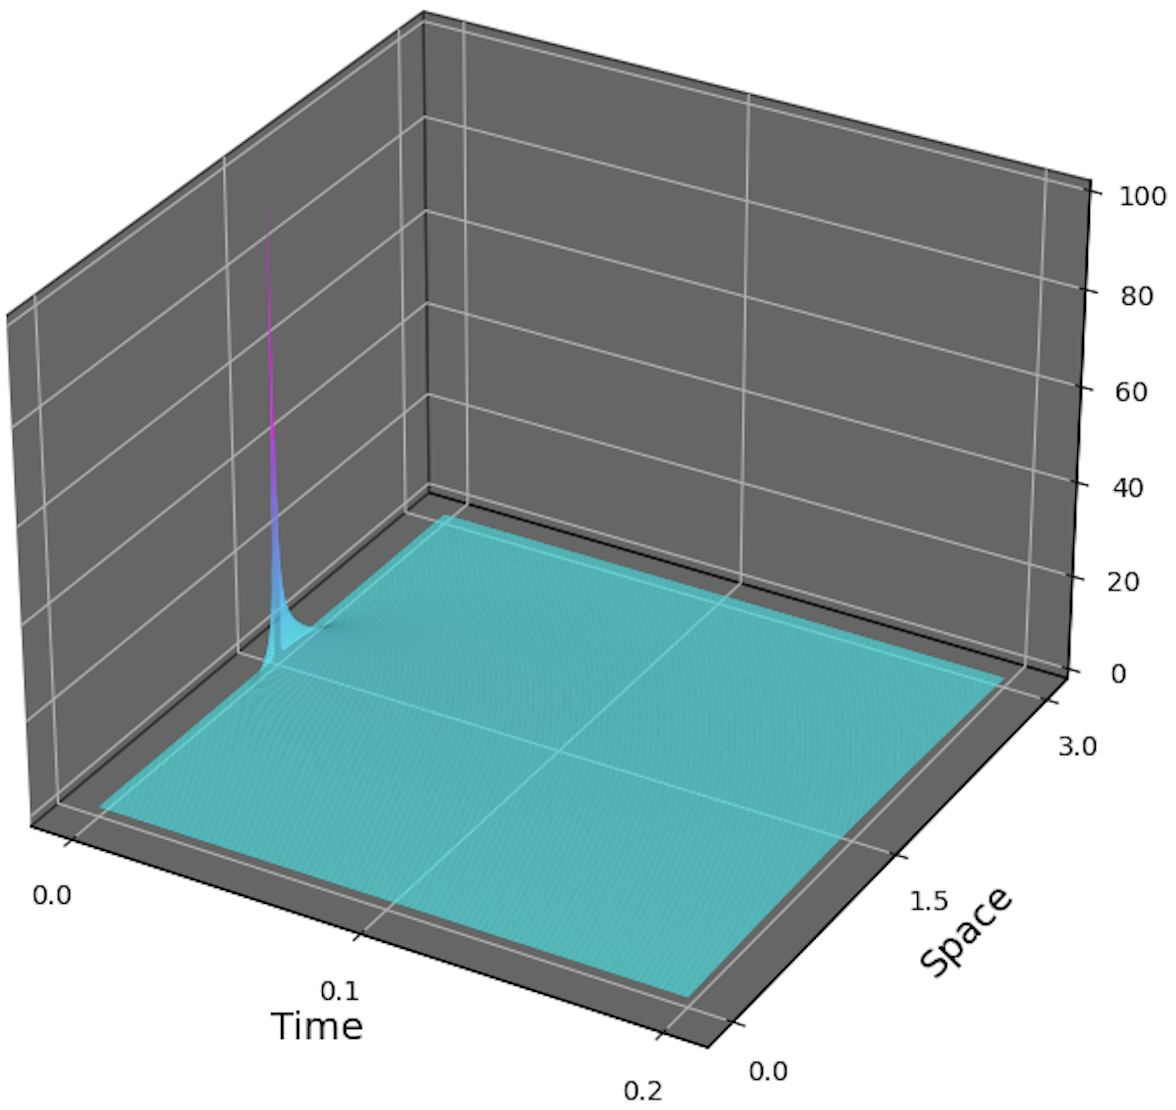
\includegraphics[width=\textwidth]{figs/deltaNoise0.png}
		\caption[]%
		{{\small $\lambda = 2.2$}} 
	\end{subfigure}
	\hfill
	\begin{subfigure}[b]{0.475\textwidth}   
		\centering 
		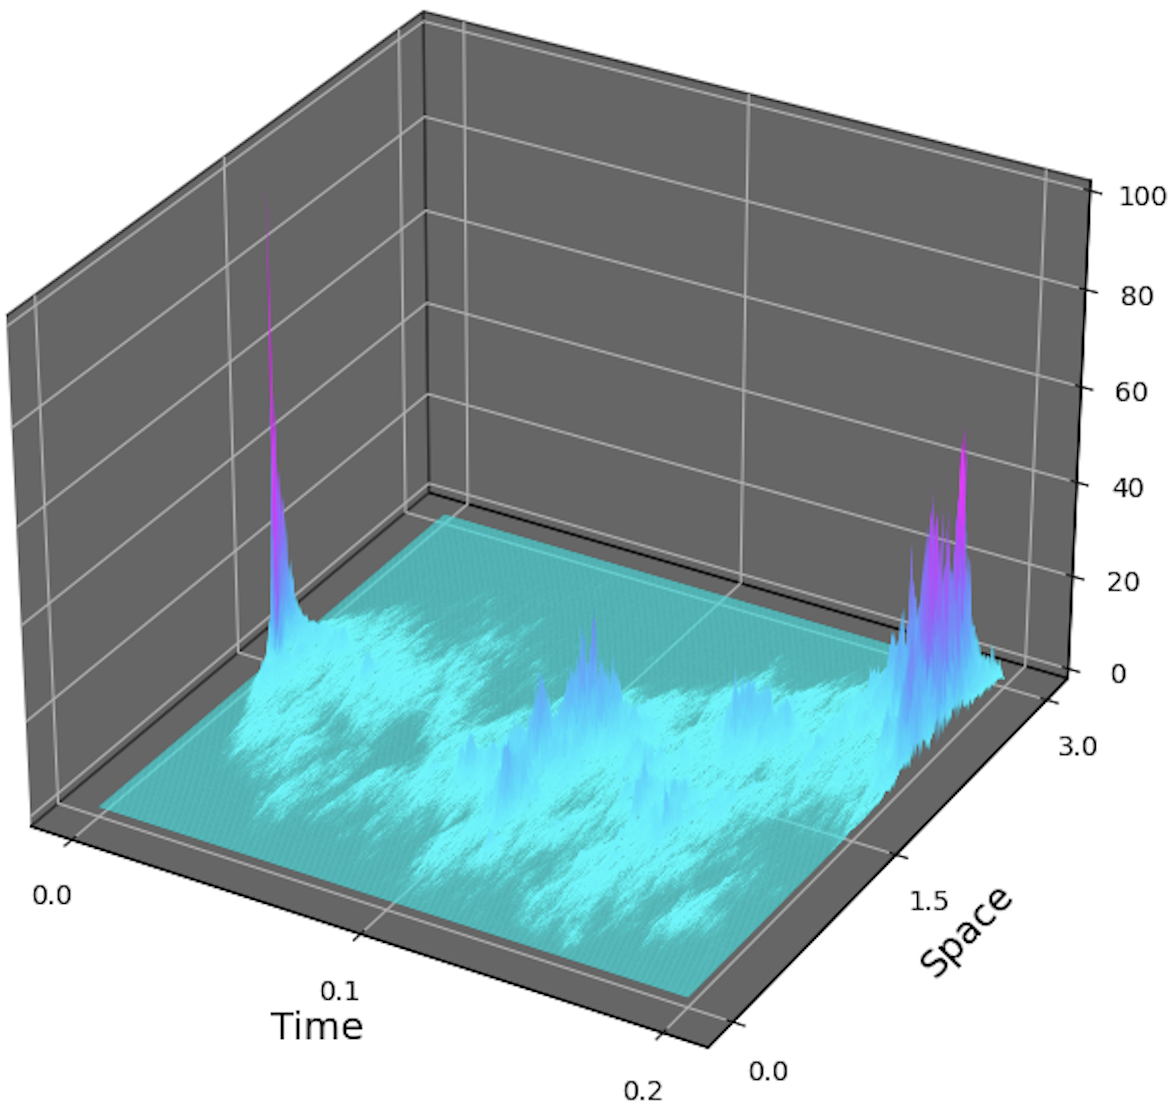
\includegraphics[width=\textwidth]{figs/deltaNoise1.8.png}
		\caption[]%
		{{\small $\lambda = 2.8$}}    
	\end{subfigure}
	\caption[] 
	{\small Simulations of Equation \eqref{E:introSHE} with $d=1$, $\zeta(\cdot) = \delta_0(\cdot)$ and $b(u) = \lambda u$.} 
	\label{Fig:SHEsim2}
\end{figure}

Following Walsh \cite{walsh:86:introduction}, we incorporate the noise into our system in the following way: 
	\begin{equation}\label{E:introSHE}
\begin{cases}
\dfrac{\partial u}{\partial t}(t,x) - \dfrac{\partial^2 u}{\partial x^2}(t,x  = b(u(t,x))\dot{W}(t,x) & t \ge 0, \; x \in \R^d \\
u(0,x) = \zeta(x) & x \in \R^d,
\end{cases}
\end{equation}
where we assume the diffusion term $b$ to be Lipschitz continuous with Lipschitz constant $L_b$. The above equation is purely notational and can be legitimately interpreted as the following stochastic integral equation:
	\begin{equation} \label{E:introMsol}
u(t,x) = \int_{\R^d} G(t, x-y)\zeta(y) \ud y + \int_0^t \int_{\R^d} G(t-s, x-y) b(u(s,y)) W(\ud s, \ud y),
\end{equation}
where the stochastic integral above is the {\em Walsh integral} and $G(t,x)$ is the Gaussian heat kernel
\[
G(t,x) = \frac{\exp\left(- \frac{|x|^2}{2t}\right)}{\sqrt{2 \pi t}}, \quad t > 0, \; x \in \R^d.
\]
Equation \ref{E:introSHE} is referred to as the {\em stochastic heat equation} (SHE) and is a widely studied stochastic partial differential equation, see for example \cite{khoshnevisan:14:analysis, walsh:86:introduction, chen.dalang:13:moments, chen.dalang:14:holder-continuity, carmona.molchanov:94:parabolic, hu.huang.ea:16:on, balan.chen:18:parabolic} and also Chapter \ref{Ch:InvMeas} below where we prove the existence of an invariant measure for the stochastic heat equation. 

   \begin{figure}
	\centering
	\begin{subfigure}[b]{0.475\textwidth}
		\centering
		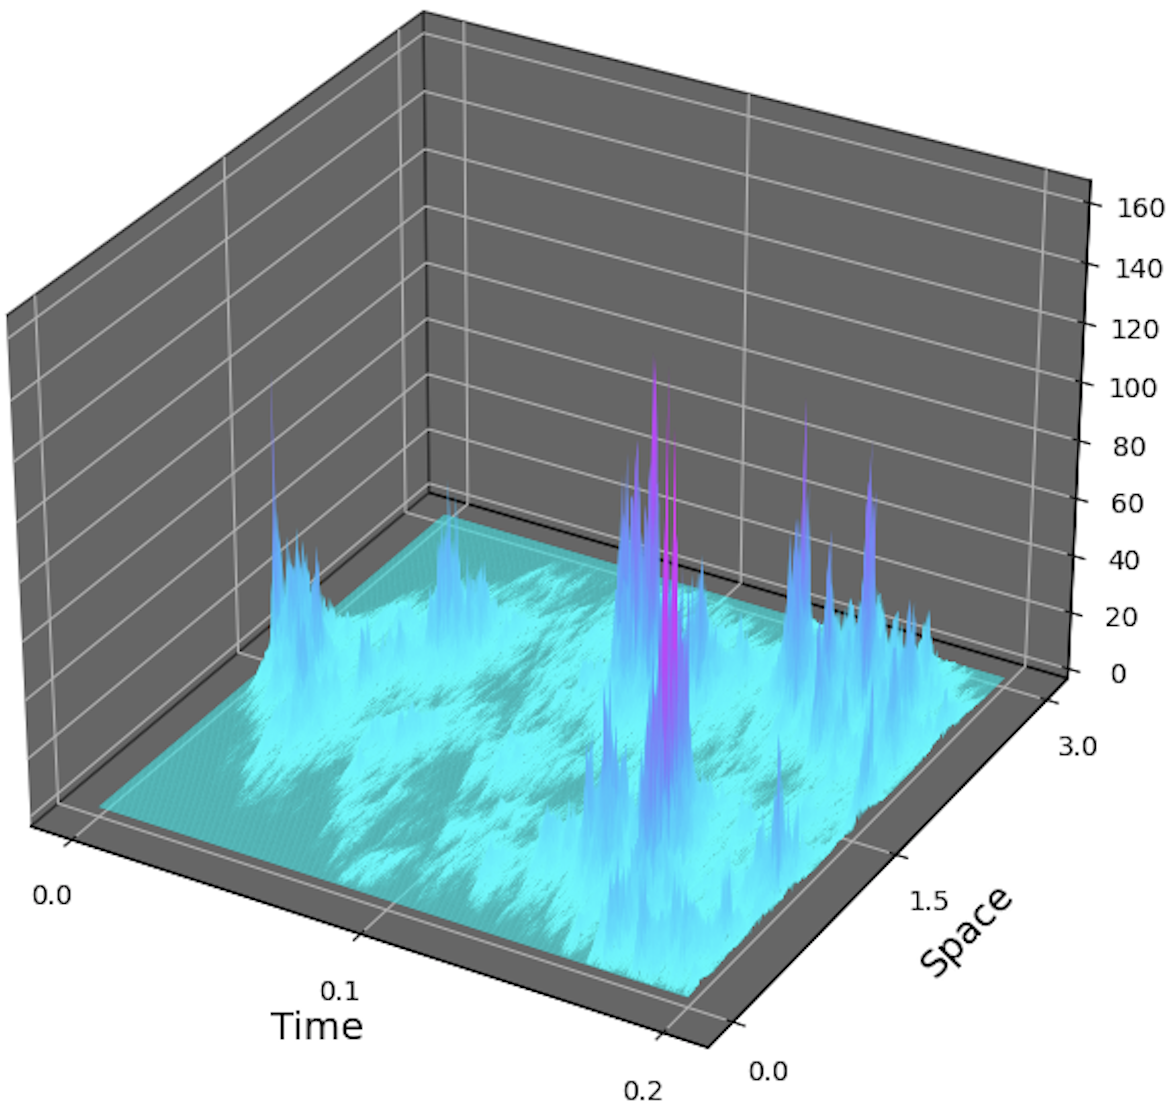
\includegraphics[width=\textwidth]{figs/deltaNoise2.2.png}
		\caption[]%
		{{\small $\lambda = 0$}}    
	\end{subfigure}
	\hfill
	\begin{subfigure}[b]{0.475\textwidth}  
		\centering 
		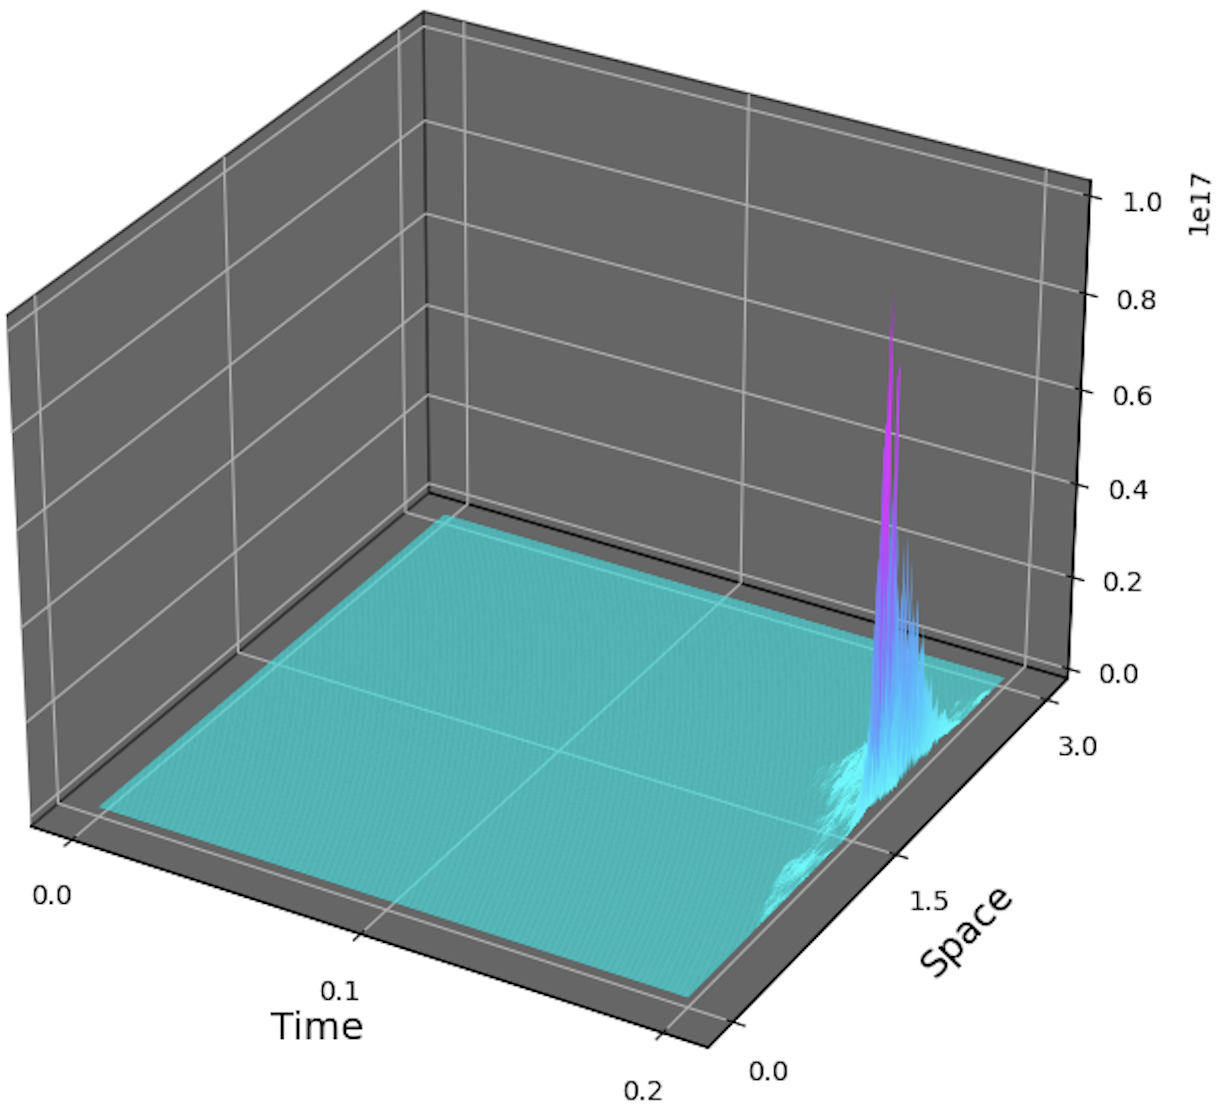
\includegraphics[width=\textwidth]{figs/deltaNoise2.8.png}
		\caption[]%
		{{\small $\lambda = 1.8$}}    
	\end{subfigure}
	\caption[] 
	{\small Simulations of Equation \eqref{E:introSHE} with $d=1$, $\zeta(\cdot) = \delta_0(\cdot)$ and $b(u) = \lambda u$.} 
	\label{Fig:SHEsim1}
\end{figure}

%\begin{figure}
%	\centering
%	\begin{subfigure}[b]{0.475\textwidth}   
%		\centering 
%		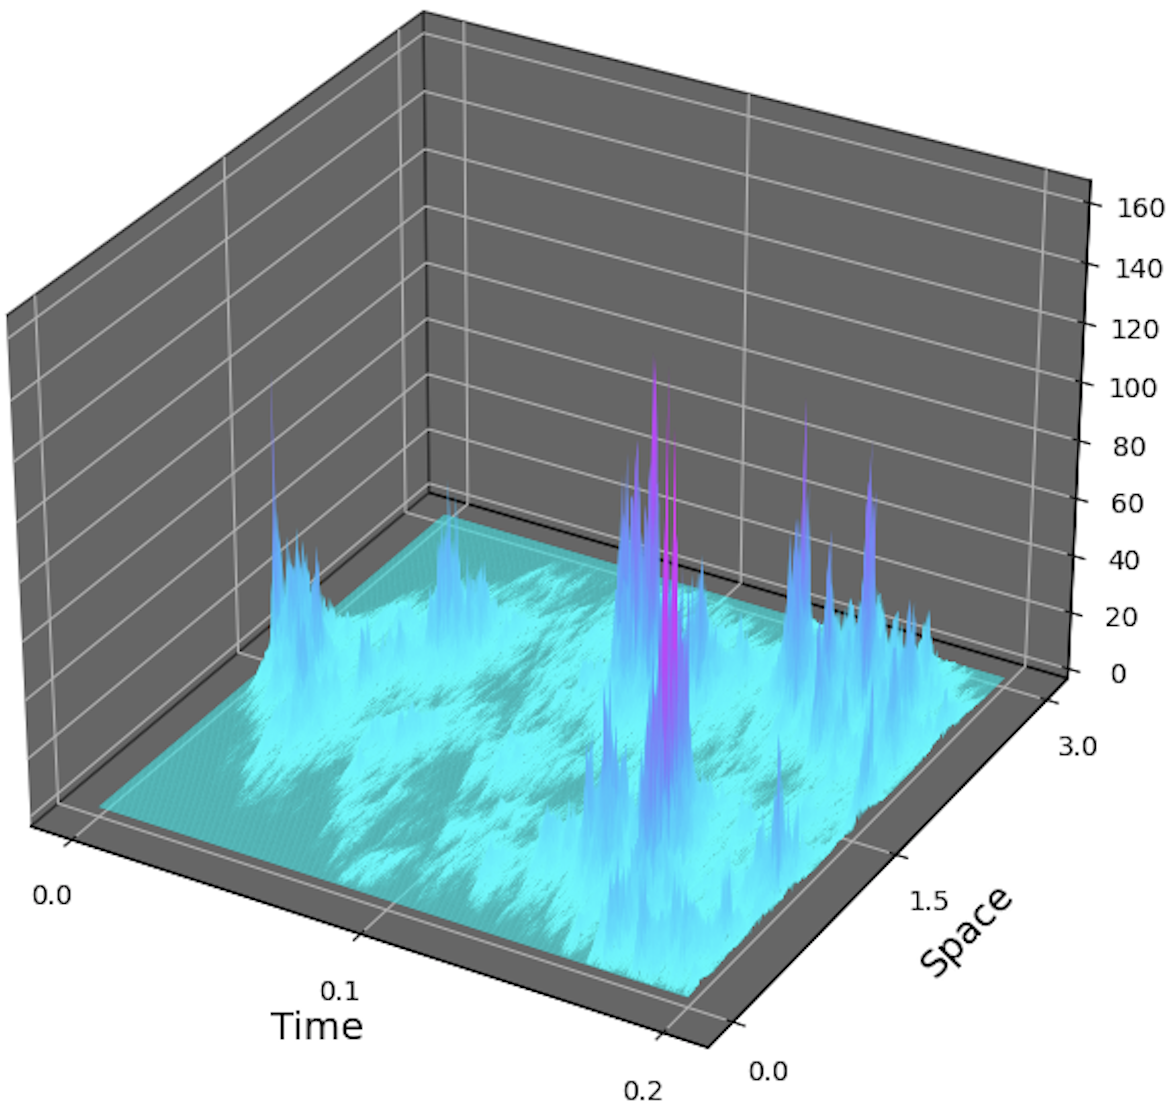
\includegraphics[width=\textwidth]{figs/deltaNoise2.2.png}
%		\caption[]%
%		{{\small $\lambda = 2.2$}} 
%	\end{subfigure}
%	\hfill
%	\begin{subfigure}[b]{0.475\textwidth}   
%		\centering 
%		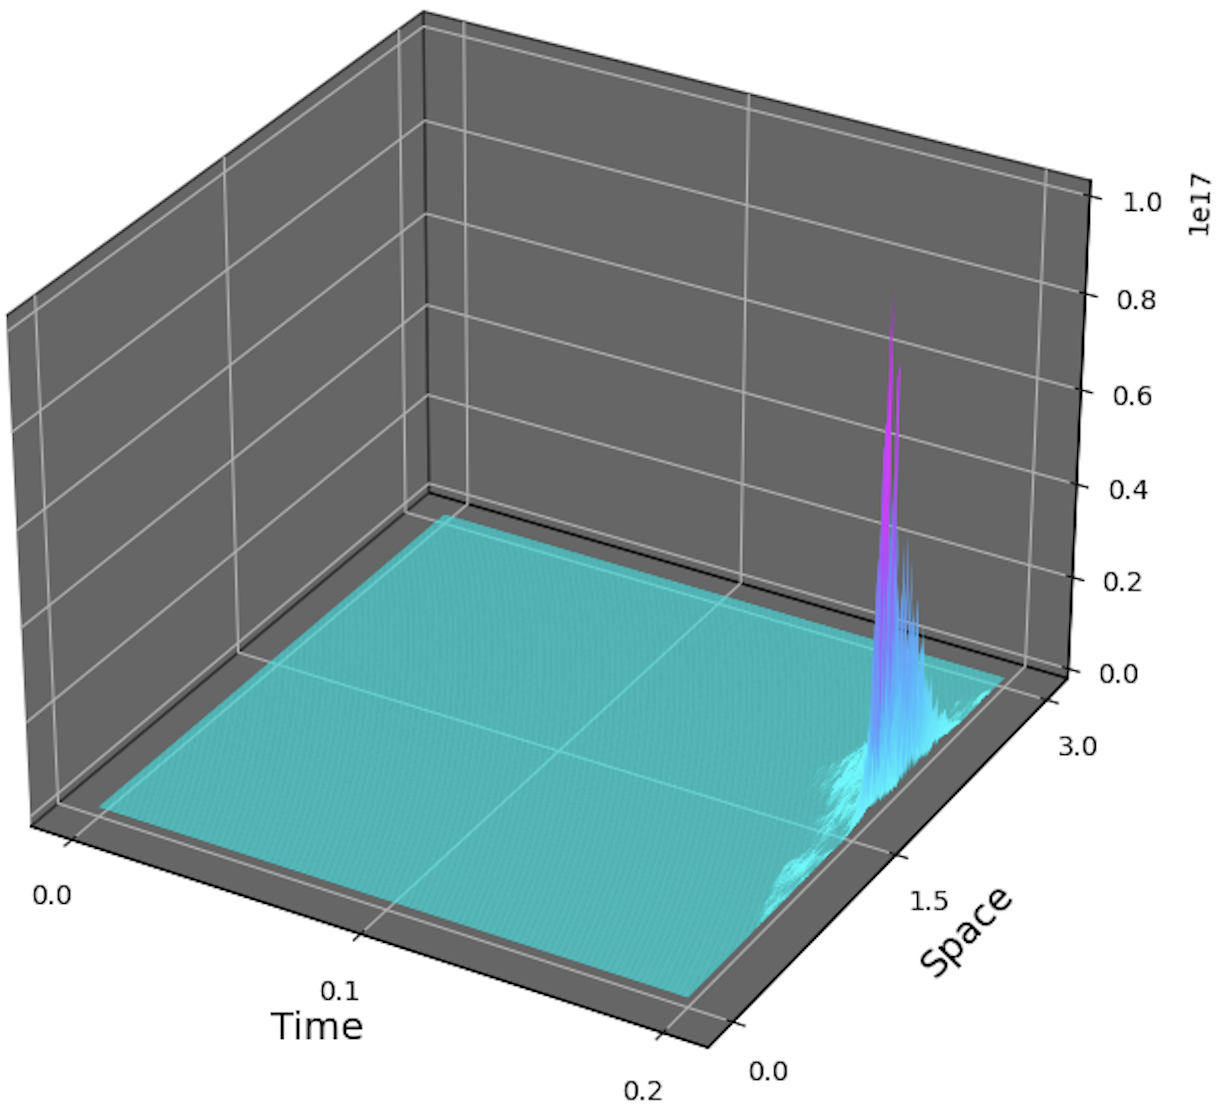
\includegraphics[width=\textwidth]{figs/deltaNoise2.8.png}
%		\caption[]%
%		{{\small $\lambda = 2.8$}}    
%	\end{subfigure}
%	\caption[] 
%	{\small Simulations of Equation \eqref{E:introSHE} with $d=1$, $\zeta(\cdot) = \delta_0(\cdot)$ and $b(u) = \lambda u$.} 
%	\label{Fig:SHEsim2}
%\end{figure}

The noise term, $\dot{W}$, brings fundamental changes to the solution $u(t,x)$ which can be seen from the simulations in Figures \ref{Fig:SHEsim1} and \ref{Fig:SHEsim2}. In particular, one can notice that as we increase $\lambda$, or the level of noise that we allow in our system, then the formation of taller and taller peaks begin to form. This phenomena is referred to as {\em intermittency}, see \cite{chen.kim:19:nonlinear, khoshnevisan.kim:15:non-linear, carmona.molchanov:95:stationary}. This concept will be one of the main focuses of my first project which is presented in Chapter \ref{Ch:ISHWEmom} below.

	   \begin{figure}[b]
	\centering
	\begin{subfigure}[b]{0.32\textwidth}
		\centering
		
\includegraphics[width=\textwidth]{figs/Yb.5.png}
		\caption[]%
		{b = .5}    
	\end{subfigure}
	\hfill
	\begin{subfigure}[b]{0.32\textwidth}
		\centering
		
\includegraphics[width=\textwidth]{figs/Yb1.png}
		\caption[]%
		{b = 1}    
	\end{subfigure}
	\hfill
	\begin{subfigure}[b]{0.32\textwidth}  
		\centering 
		
\includegraphics[width=\textwidth]{figs/Yb1.9.png}
		\caption[]%
		{b = 1.9}    
	\end{subfigure}
	\caption[] 
	{\small Some plots of $G_{2,b,0,2,1}(t,x)$ with $-4 \le x \le 4$ and $1 \le t \le 4$.} 
	\label{Fig:FoxSurface}
\end{figure}

\subsection{A brief overview of the first project}
In the following chapter we will study the following space-time fractional stochastic partial differential equation driven by a {\em time-independent noise} $\dot{W}(x)$ that interpolates both the stochastic heat and wave equations:
\begin{equation} \label{E:IntroISHWE}
\begin{cases}
\left(\partial^b_t + \frac{\nu}{2}(-\Delta)^{a/2}\right)\: u(t,x) = I^r_t \left[\sqrt{\theta}\: u(t,x)\: \dot W(x) \right] & \text{$x\in \R^d$, $t>0$}, \\
u(0,\cdot) = 1                                                                                                             & b \in (0,1],               \\
u(0,\cdot) = 1, \quad \partial_t u(0,\cdot) = 0                                                                            & b \in (1,2),
\end{cases}
\end{equation}
where $\partial^b_t $ is the {\em Caputo} derivative, $(-\Delta)^{a/2}$ is the {\em fractional Laplacian} and $I^r_t$ is the {\em Riemann-Liouville fractional integral}. Similar to the stochastic heat equation above, \eqref{E:IntroISHWE} is understood through the  following stochastic integral equation:
	  \begin{equation} \label{E:IntroISHWEmild}
	u(t,x) = 1 + \sqrt{\theta}\int_0^t \left( \int_{\R^d} G(t-s,x-y)u(s,y) W(\delta y) \right)\ud s,
	\end{equation}
where, because of the choice of noise, the stochastic integral above is the {\em Skorohod} integral \cite{nualart.nualart:18:introduction} and here $G = G_{a, b, r, \nu, d}$ is the fundamental solution which is given through the Fox H-function (see Figures \ref{Fig:FoxSurface} and \ref{Fig:FoxCross} and \cite[Theorem 4.1]{chen.hu.ea:19:nonlinear}). One can see that when $a=2$, $b=1$ and $r=0$ then \eqref{E:IntroISHWE} reduces to the stochastic heat equation and when $a=b=2$ and $r=0$ then it reduces to the stochastic wave equation.

\begin{figure}[t]
	\centering
	
\includegraphics[scale=.8]{figs/Ybt1.png}
	\caption[] 
	{\small Cross sections of $G_{2,b,0,2,1}(t,x)$ with $-4 \le x \le 4$ and $t = 1$.} 
	\label{Fig:FoxCross}
\end{figure}

An important key feature of the solution, which is due to the choice of noise and simplified initial conditions, is the following Wiener Chaos expansion of the solution 
\begin{equation} \label{E:IntroISHWEwcexp}
u(t,x) = 1 + \sum_{k=1}^\infty \theta^{k/2}I_k(f_k(\cdot,x,t)),
\end{equation}
where $I_k$ denotes the $k^{th}$ order Skorohod integral and the kernels $f_k$ are calculated through a standard Picard iteration procedure (see the discussion after Definition \ref{D:Sol} below). Because of an orthogonality result that is exhibited by the integrals $I_k$ (e.g. \cite[Equation 4.1]{nualart.nualart:18:introduction}), one may deduce the following useful expression for the second moment of the solution (see Theorem \ref{T:2momseries} below):
\[
	    \mathbb{E}\left(u(t,x)^2\right)
	= \sum_{n \ge 0} \theta^n n!  \Norm{\widetilde{f_n}(\cdot,x,t)}_{\mathcal{H}^{\otimes n}}^2
	\quad \text{for all $(t,x) \in (0,T) \times \R^d$}.
\]

The main goals will be to prove existence and uniqueness of the solution (Theorem \ref{T:solvable}) and to calculate the following limits:
	\[
		\lim_{t \to \infty} t^{-\beta} \log \E\left(|u(t,x)|^p\right) 
		\quad \text{and} \quad 
		\lim_{p \to \infty} p^{-\beta} \log \E\left(|u(t,x)|^p\right),
	\]
where $\beta$ is a constant that is to be determined (see Theorem \ref{T:asym} and Corollary \ref{C:Lim}). One should note that both the positivity and the finiteness of the above limits imply that the following functions exhibit exponential growth:

\[
t \mapsto \E\left(|u(t,x)|^p\right) 
\quad \text{and} \quad
p \mapsto \E\left(|u(t,x)|^p\right).
\]
The calculation of these limits is a very long an lengthly process so we hold any further discussion until Chapter \ref{Ch:ISHWEmom}.


However, as for the solvability of \eqref{E:IntroISHWE}, we prove that the solution may uniquely exist either {\em globally} or {\em locally}. We say a global solution exists if for any $p \ge 2$, $x \in \R^d$ and $t>0$, the $p^{th}$ moment, $\Norm{u(t,x)}_p$, exists. On the other hand, we say that a local solution exists when there exists two times $T_{1,p} < T_{2,p}$ such that for any $p \ge 2$ and $x \in \R^d$, the $p^{th}$ moment exists for $t<T_{1,p}$ and blows up for $t > T_{2,p}$. We prove that $T_{1,2} = T_{2,2}$ and in addition, for any $p \ge 2$, we calculate $T_{1,p}$ and give precise conditions on when a solution will be global or local. It is worth mentioning that the calculation of the cutoff time, $T_{1,p}$, is only possible due to our ability to express the solution in terms of its Wiener Chaos expansion as in \eqref{E:IntroISHWEwcexp}.

\subsection{A brief overview of the second project}
In the final chapter, we will turn our focus towards proving the existence of an invariant measure for the stochastic heat equation \eqref{E:introSHE} on the whole space $\R^d$. Equations such as the SHE can be used by researchers to describe dynamical systems. Moreover, there often is a strong need to know the ergodic behavior of the dynamical system and no ergodic behavior can exists without an invariant measure. Hence proving the existence of such a measure is a crucial starting point. 

Since we work on the whole space, one needs to introduce a positive, bounded and continuous weight $\rho \in L^1(\R^d)$ and the corresponding $\rho$-weighted space of square integrable functions $L^2_{\rho}(\R^d)$ (see Section \ref{SS:Weight}). We will see below in Theorem \ref{T:Lrho}, that the solution starting from $\mu$, which we denote as $u(t,\cdot; \mu)$, is almost surely in this weighted space for a broad range of initial data which includes all bounded functions, some unbounded functions such as $|x|^{-\alpha}$ with $0 < \alpha < d/2$ and even measures such as the Dirac delta measure.

A crucial property of the system that must be exhibited for an invariant measure to exist is the {\em Markov property}. Essentially this means that one must be able to stop and restart their system whenever they choose and that the system then must act the same as it would if it were allowed to run uninterrupted. It makes sense that the SHE would satisfy this property since heat always moves from hot to cold. Thus no matter when we restart our system, the transfer of heat will just continue as if nothing happened. 

However, this restart property is not always satisfied. Consider the situation where we pull back a string that is tightly secured at both end points. When we release the string, it will vibrate back and fourth until it loses its momentum and ends back at rest. The problem that presents itself here is that two vibrating strings could have the same position but different velocities (see Figure \ref{Fig:stringstop}). 

\begin{figure}[!htbp]
\begin{center}
	\newbox\qbox
	\setbox\qbox\hbox{?}
	\edef\qmarkHeight{\the\ht\qbox}
	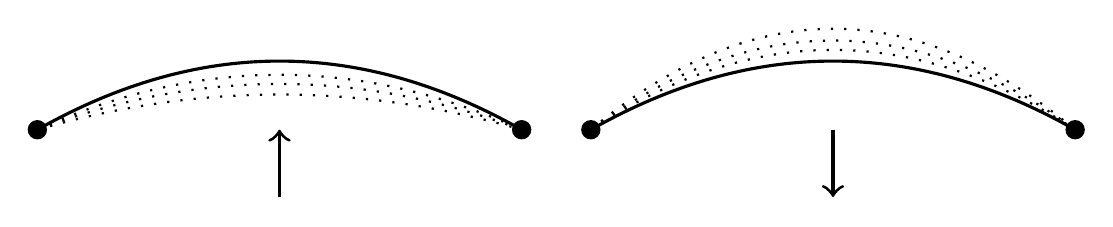
\begin{tikzpicture}[scale = 2]
\begin{axis}[
axis lines=none,
xmin=-.3, xmax=15.3,
ymin=-4, ymax=4,
domain=0:7,samples=200,
]

\addplot [black, line width=.2mm, domain=0:7
] {x*(7-x) / 20};

\addplot [black, dotted, domain=0:7
] {x*(7-x) / 25};

\addplot [black, dotted, domain=0:7
] {x*(7-x) / 30};

\addplot [black, dotted, domain=0:7
] {x*(7-x) / 39};


%%%%%%%%%%%%

\addplot [black, line width=.2mm, domain=8:15
] {(x-8)*(15-x) / 20};

\addplot [black, dotted, domain=8:15
] {(x-8)*(15-x) / 17.2};

\addplot [black, dotted, domain=8:15
] {(x-8)*(15-x) / 15.4};

\addplot [black, dotted, domain=8:15
] {(x-8)*(15-x) / 13.6};


\fill (0,0) circle (1.75pt);
\fill (7,0) circle (1.75pt);
\fill (8,0) circle (1.75pt);
\fill (15,0) circle (1.75pt);

\draw[->, line width=.2mm] (3.5,-.6) -- (3.5,0);
\draw[->, line width=.2mm] (11.5,0) -- (11.5,-.6);
\end{axis}

\end{tikzpicture} 
\end{center}
\caption{A still shot of two vibrating strings at the same position but moving in opposite directions.}
\label{Fig:stringstop}
\end{figure}

\noindent For example, suppose we froze both strings illustrated above. When we initiate the restart, both stings will not continue as they were prior to the restart. What will happen is that they both will start moving in the direction of least resistance (see Figure \ref{Fig:stringstart}).  
\begin{figure}[!htbp]
\begin{center}
	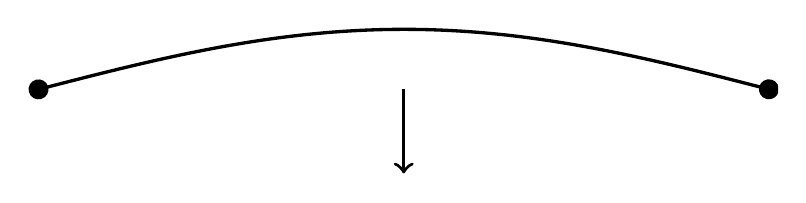
\begin{tikzpicture}[scale = 1.5]
	\begin{axis}[
	axis lines=none,
	xmin=-.3, xmax=3.18,
	ymin=-4, ymax=4,
	domain=0:3.14,samples=500,
	]
	
	\addplot [black,thick,
	postaction={decorate, decoration={markings, 
			mark=at position 0 with {\fill circle(2pt);},
			mark=at position 1 with {\fill circle(2pt);}
	}}
	]  {sin(deg(x))/1.4};
	\draw[->, thick] (1.57,0) -- (1.57, -1); 
	\end{axis}
	\end{tikzpicture} 
\end{center}
\caption{Direction of movement when re-releasing the string, regardless of the prior velocity.}
\label{Fig:stringstart}
\end{figure}
\noindent Thus the system will appear differently as it would if it were never restarted at all. This heuristically shows us that this system can not satisfy the Markov property and therefore an invariant measure will not exist in this setting.


We define the probability laws of the solution as
	\[
	\mathscr{L}(u(t,\cdot;\zeta))(A) = \mathbb{P} \left[ \omega \in \Omega: u(t,\cdot; \zeta)(\omega) \in A \right], \quad A\in \mathscr{B}(L^2_{\rho}(\R^d)),
	\]
where $\mathscr{B}(L^2_{\rho}(\R^d))$ denotes the Borel subsets of $L^2_{\rho}(\R^d)$. Because of the Markov property of the solution, the laws form a family of {\em Markovian transition functions}, $P_t(\zeta, A) := \mathscr{L}(u(t,\cdot;\zeta))(A)$, for $\zeta \in L^2_{\rho}(\R^d)$. Moreover, the transition functions form a {\em transition semi-group} defined as follows:
	\[
		P_t\varphi(x) = \int_{L^2_{\rho}(\R^d)} P_t(x, \ud y) \varphi(y), \quad \varphi \in \mathcal{B}(L^2_{\rho}(\R^d)),
	\]
 where $\mathcal{B}(L^2_{\rho}(\R^d))$ denotes the bounded Borel measurable functions on $L^2_{\rho}(\R^d)$. 
 
 With this said, we say that a probability measure, $\eta$, on $\mathscr{B}(L^2_{\rho}(\R^d))$ is {\em invariant} for \eqref{E:introSHE} when the following holds:
\begin{equation}\label{E:IntroInvMeas2}
\int_{L^2_{\rho}(\R^d)} P_t\varphi(x)\eta(\ud x) = \int_{L^2_{\rho}(\R^d)} \varphi(x) \eta(\ud x),
\quad \text{for all $ t\ge 0$ and $\varphi \in \mathcal{B}(L^2_{\rho})(\R^d)$ }.
\end{equation} 
Recall that by definition $P_0\varphi(x) = \varphi(x)$ and so \eqref{E:IntroInvMeas2} is essentially saying that the transition semi-group is {\em time-invariant} with respect to the invariant measure $\eta$. We mention that this is a key feature of ergodicity. 

We should also mention now that there is an equivalent way that one can define the invariant measure, and in fact it is the definition that we will choose to use for the remainder of this thesis. Any probability measure, $\eta$, on the Borel $\sigma$-field $\mathscr{B}(L^2_{\rho}(\R^d))$ is said to also be invariant for \eqref{E:introSHE} if
\begin{equation}\label{E:IntroInvMeas}
\eta(A) = \int_{L^2_{\rho}(\R^d)} \mathscr{L}(u(t,\cdot;\zeta))(A) \; \eta(\ud \zeta),
\quad \text{for all $ t\ge 0$ and $A\in \mathscr{B}(L^2_{\rho})(\R^d)$}.
\end{equation} 
For more on these equivilent definitions, we direct the reader to \cite[Section 11.1]{da-prato.zabczyk:14:stochastic}.

Tessitore and Zabczyk laid forth a schematic to prove the existence of an invariant measure in \cite{tessitore.zabczyk:98:invariant}, which revolves around showing the following:
\begin{enumerate}
	\item the probability laws of the solution form a family of {\em Markovian transition functions},
	\item  the solution, $u(t,x;\mu)$, satisfies a boundedness in probability condition.
\end{enumerate}
Moreover, when one verifies the above steps, then by applying the Krylov–Bogoliubov existence theorem (\cite[Theorem 11.7]{da-prato.zabczyk:14:stochastic}), it can be shown that the invariant measure, $\eta$, takes the following form:
	\begin{equation} \label{E:IntroInvMeasForm}
	\eta(A) = \lim_{n \to \infty} \frac{1}{T_n} \int_{t_0}^{T_n + t_0} \mathscr{L}(u(t,\cdot; \mu))(A) \ud t, \quad A \subset \mathscr{B}(L^2_{\rho}(\R^d)),
	\end{equation}
where $\{T_n\}_{n\ge 1}$ is an appropriately chosen sequence with $T_n\uparrow \infty$ and where $\mathscr{B}(L^2_{\rho}(\R^d))$ (see Theorem \ref{T:Main} below).

Note that we already discussed that the first item above is satisfied in our setting. On the other hand, the second item will require some effort to show. A sufficient condition that implies this boundedness condition is the following:
	\begin{align} \label{E:IntroBddMnt}
	\sup_{t>0} \E\left(\Norm{u(t,\cdot)}_{\rho}^2\right)
	<\infty.
	\end{align}
We remind the reader that for the SHE, moments usually grow exponentially in time (e.g. see \cite[Theorem 1.3]{chen.kim:19:nonlinear}), and so for the above finiteness to occur we will need additional assumptions (e.g. see Equation \eqref{E:U0finite} below). 

In fact, in order for Tessitore and Zabczyk to provide a specific scenario where an invariant measure exists (e.g. \cite[Theorem 3.3]{tessitore.zabczyk:98:invariant}), they had to significantly strengthen their assumptions and require the following:
 \begin{equation} \label{E:IntroTZspec}
d\ge 3 \quad \text{and} \quad
L_b^{-2}> \frac{\Gamma(d/2 -1)2^{d/2-2}}{(2\pi)^{2d}} \int_{\R^d} \left(\left|  \mathcal{F}\left(\sqrt{ \widehat{f}\: }\right) \right| * \left| \mathcal{F}\left(\sqrt{ \widehat{f}\: }\right)\right|\right) (\zeta) |\zeta|^{2-d} \ud \zeta,
\end{equation}
where $L_b$ is the Lipschitz constant of the drift term and $\hat{f}$ is the spectral density of the noise (see Section \ref{SS:TessZabz} below). Moreover, under this strengthened assumption, they proved that there exists an invariant measure for the SHE starting from the constant $1$ initial condition (e.g. \eqref{E:introSHE} with $\zeta(x) = 1$). However, due to its complexity, \eqref{E:IntroTZspec} was not calculated for any specific $\widehat{f}$ and without being able to do so, one may not apply this result for a specific noise. This is clearly a huge set back as picking the noise of your system is the main reason one would want to study a SPDE.

Our results vastly improve on this as we provide much simpler and more easily verifiable conditions in our Theorem \ref{T:Main} below that will guarantee the existence of an invariant measure. Moreover in Section \ref{SS:Bassel}, we are able to give specific examples of spectral densities, $\widehat{f}$, that satisfy the conditions of our Theorem \ref{T:Main}. In addition, in Section \ref{SS:Init} we enlarge the space of initial conditions to include all bounded functions, some unbounded functions and even some measures such as the Dirac delta measure. 

\chapter{ \normalfont Exact Moment Asymptotics for the Interpolated Stochastic Heat and Wave Equation} \label{Ch:ISHWEmom}
\section{Introduction and main results}
In this chapter we study the following {\it stochastic partial differential equation} (SPDE) with 
fractional differential operators:
\begin{equation} \label{E:SPDE}
\begin{cases}
\left(\partial^b_t + \frac{\nu}{2}(-\Delta)^{a/2}\right)\: u(t,x) = I^r_t \left[\sqrt{\theta}\: u(t,x)\: \dot W(x) \right] & \text{$x\in \R^d$, $t>0$}, \\
u(0,\cdot) = 1                                                                                                             & b \in (0,1],               \\
u(0,\cdot) = 1, \quad \partial_t u(0,\cdot) = 0                                                                            & b \in (1,2),
\end{cases}
\end{equation}
where $a \in (0,2]$, $b \in (0,2)$, $r\ge 0$, $\nu > 0$ and $\theta>0$. Here the noise $W = \left\{
W(\phi) : \phi \in \mathcal{D}(\R^d) \right\}$ is a centered and time-independent Gaussian process,
defined on a complete probability space $(\Omega, \mathcal{F}, P)$, with mean zero and covariance
\begin{align*}
\mathbb{E}\left[ W(\phi) W(\psi) \right] = \int_{\R^d} \mathcal{F}\phi(\xi)\overline{\mathcal{F}\psi(\xi)} \mu(\ud \xi) =: \langle \phi, \psi \rangle_{\mathcal{H}},
\end{align*}
where $\mu$ refers to the {\it spectral measure}, which is assumed to be a nonnegative and
nonnegative definite tempered measure on $\R^d$. Let $\gamma$ be the Fourier transform of $\mu$ (see
Section \ref{SS:Malliavin}), which is also a nonnegative and nonnegative definite measure on $\R^d$
thanks to Bochner's theorem. Throughout the paper, we use $\mathcal{F}\phi(\xi) = \int_{\R^d}
\exp(-ix \xi) \phi(x) \ud x$ to denote the Fourier transform of a test function $\phi$.

In \eqref{E:SPDE}, $(-\Delta)^{a/2}$ refers to the {\it fractional Laplacian} of order $a$,
$\partial^b_t$ denotes the {\it Caputo fractional differential operator}
\begin{align*}
\partial^b_tf(t) :=
\begin{cases}
\dfrac{1}{\Gamma(m-b)} \int_0^t \ud \tau \dfrac{f^{(m)}(\tau)}{(t-\tau)^{b+1-m}} & \text{if } m-1 < b < m, \bigskip \\
\dfrac{\ud^m}{\ud t^m}f(t)                                                       & \text{if } b=m,
\end{cases}
\end{align*}
where $m$ is an integer, and $I^r_t$ refers to the {\it Riemann-Liouville fractional integral} of
order $r>0$
\begin{align*}
I^r_tf(t) := \frac{1}{\Gamma(r)} \int_0^t (t-s)^{r-1}f(s)\ud s, \quad \text{for } t>0,
\end{align*}
with the convention that when $r=0$, $I^0_t = \text{Id}$ reduces to the identity operator. The
fundamental solution to \eqref{E:SPDE} is expressed explicitly in terms of the {\it Fox H-function},
$H^{m,n}_{p,q}(z)$, which is much more complicated than the Green's function for either the heat or
wave equation. We denote the fundamental solution as
\begin{equation} \label{E:GreenFunction}
G(t,x):= G_{a,b,r,\nu,d}(t,x),
\end{equation}
where
\[
G_{a,b,r,\nu,d}(t,x) = \pi^{-d/2} |x|^{-d} t^{b+r-1} H^{2,1}_{2,3}\left( \frac{|x|^a}{2^{a-1}\nu t^b}\;  \Bigg \vert  \begin{array}{l}
(1,1),\; (b+r,b) \\
(d/2,a/2),\; (1,1),\; (1,a/2)
\end{array} \right).
\]
We direct the reader to Theorem 4.1\footnote{$G(t,x)$ corresponds to $Y_{a,b,r,\nu,d}(t,x)$ from
	\cite{chen.hu.ea:19:nonlinear}.} of \cite{chen.hu.ea:19:nonlinear} for more details. Since we are interested in the constant one initial
condition (and zero initial velocity when $b>1$), Theorem 4.1 ({\it ibid.}) implies that the
corresponding solution to the homogeneous equation (i.e. the solution when there is no driving
source) is equal to the constant one. Hence through superposition, \eqref{E:SPDE} can be written as
the following stochastic integral equation:
\begin{equation} \label{E:spdeint}
u(t,x) = 1 + \sqrt{\theta}\int_0^t \left( \int_{\R^d}G(t-s,x-y)u(s,y) W(\delta y) \right) \ud s,
\end{equation}
where the stochastic integral is in the {\it Skorohod} sense; see Definition \ref{D:Sol} below.  In
the following, the fundamental solution will exclusively refer to $G(t,x)$, which is indeed a smooth
function for $x\ne 0$. Our results rely on the following assumption for the nonnegativity of
$G(t,x)$:

\begin{assumption}[Nonnegativity] \label{A:Nonnegative}
	Assume that the fundamental solution $G(t,x)$ is nonnegative for all $t>0$ and $x\in\R^d$.
\end{assumption}

\begin{remark} \label{R:Nonnegative}
	% Regarding the nonnegativity assumption --- Assumption \ref{A:Nonnegative},
	Thanks to Theorem 4.6 of \cite{chen.hu.ea:19:nonlinear} (see also Theorem 3.1 of \cite{chen.hu.ea:17:space-time} for the case when $r=0$),
	we have the following four groups of sufficient conditions \footnote{Note that when $d\ge 1$,
		$b=1$ and $a\in (0,2]$, part (1) of \cite[Theorem 4.6]{chen.hu.ea:19:nonlinear} says that the fundamental solution
		$Y$, which is the fundamental solution $G$ in this paper, is nonnegative provided $r=0$ or
		$r>1$. Indeed, because in this case $Z$ is always nonnegative, for $r>0$, $Y$ as a fractional
		integral of $Z$ (see (4.5), {\it ibid.}),  $Y$, or our $G$, should also be nonnegative. We thank
		Guannan Hu who pointed out to us this observation.}, under either group of which $G(t,\cdot)$ is
	nonnegative (see Figure \ref{F:Nonnegative} for an illustration) :
	\begin{enumerate}
		\item $d \ge 1$, $b\in(0,1]$, $a\in(0,2]$, $r\ge0$;
		% \item $d \ge 1$, $b=1$, $a\in (0,2]$, $r=0$ or $r>1$;
		\item $1\le d \le 3$, $1<b<a\le 2$, $r>0$;
		\item $1 \le d \le 3$, $1 < b=a < 2$, $r > \dfrac{d+3}{2}-b$.
	\end{enumerate}
\end{remark}

\begin{figure}[htpb]
	\centering
	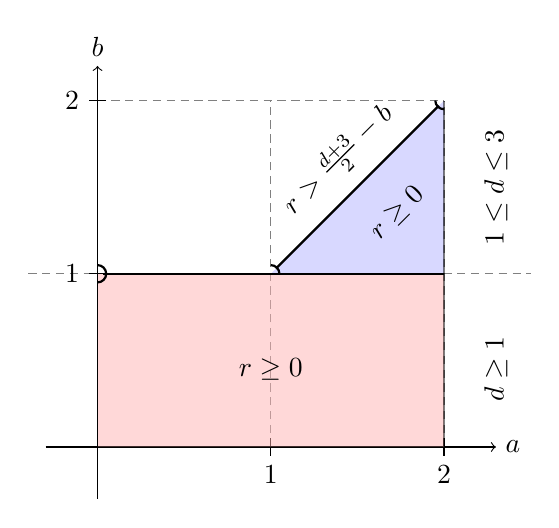
\begin{tikzpicture}[scale=2.2]
	\draw [->] (-0.3,0) -- (2.3,0) node [right] {$a$};
	\draw [->] (0,-0.3) -- (0,2.2) node [above] {$b$};
	\draw [densely dashed,gray] (1,0) -- (1,2) (2,0) -- (2,2) (-0.4,1) -- (2.5,1) (0,2) -- (2,2);
	\draw (1,0.05) -- (1,-0.05) node [below] {$1$};
	\draw (2,0.05) -- (2,-0.05) node [below] {$2$};
	\draw (0.05,1) -- (-0.05,1) node [left] {$1$};
	\draw (0.05,2) -- (-0.05,2) node [left] {$2$};
	\filldraw [fill=red!30, opacity=0.5] (0,0) rectangle (2,1);
	\filldraw [fill=blue!30, opacity=0.5] (1,1) -- (2,1) -- (2,2);
	\draw [thick] (1.03,1.03) -- (1.97,1.97);
	\draw [thick] ([shift=(0:0.05)]1,1) arc (0:90:0.05);
	\draw [thick] ([shift=(180:0.05)]2,2) arc (180:270:0.05);
	\node at (2.3,1.5) [rotate=90, anchor=center] {$1\le d\le 3$};
	\node at (2.3,0.45)[rotate=90, anchor=center] {$d\ge 1$};
	\draw [thick] (0.03,1) -- (2,1);
	\draw [thick] ([shift=(-90:0.05)]0,1) arc (-90:90:0.05);
	\node at (1.73,1.35) [rotate=45, anchor=center] {$r\ge 0$};
	\node at (1,0.45) {$r\ge 0$};
	% \node at (1,0.9) {$r=0$ or $r>1$};
	\node at (1.5,1.55) [rotate=45,anchor=south] {$r>\frac{d+3}{2}-b$};
	\end{tikzpicture}
	\caption{Illustration of the sufficient conditions (Remark \ref{R:Nonnegative}) for
		$G(t,\cdot)$ to be nonnegative.}
	\label{F:Nonnegative}
\end{figure}

Regarding the noise, we formulate the following assumption in order to cover the Riesz kernel case,
the fractional noise and a mixture of them:
\begin{assumption}[Noise] \label{A:Noise}
	Let $k \in \{1, \cdots , d\}$ and partition the $d$-coordinates of $x=(x_1, \cdots, x_d)$ into $k$
	distinct groups of size $d_i$ so that $d_1 + \cdots + d_k = d$. Denote $x_{(i)} = (x_{i_1} ,
	\cdots , x_{i_{d_i}})$ to be the coordinates in the $i^{th}$ partition. Assume that the
	correlation function of the Gaussian noise is given by
	\begin{equation}
	\label{E:corfunction}
	\gamma(x) = \prod_{i=1}^k \left|x_{(i)}\right|^{-\alpha_i} \qquad \text{with $\alpha_i \in (0, d_i)$.}
	\end{equation}
	Define $\alpha := \sum_{i=1}^k \alpha_i$.
\end{assumption}

\begin{remark}[Spectral density and decomposition] \label{R:Noise}
	Recall that the {\it spectral density} of $\gamma$ from \eqref{E:corfunction}, which by definition is
	$\mathcal{F}\gamma$, takes the following form:
	\begin{equation}
	\label{E:specfunction}
	\mu (\ud \xi) = \varphi(\xi) \ud \xi \quad \text{with} \quad
	\varphi(\xi) = \prod_{i=1}^k C_{\alpha_i,d_i} |\xi_{(i)}|^{-(d_i-\alpha_i)}.
	\end{equation}
	Moreover, in the derivations below, we need to find a nonnegative and nonnegative definite $K$
	such that $\gamma = K*K$ where `$*$' denotes the spatial convolution. Indeed, one can choose
	\begin{align}
	\label{E:K}
	K(x) =\prod_{i=1}^k \beta_{\alpha_i,d_i} \left|x_{(i)}\right|^{-(d_i+\alpha_i)/2}.
	\end{align}
	The two constants in both \eqref{E:specfunction} and \eqref{E:K} are defined as
	\begin{equation}
	\label{E:noiseconstant}
	C_{\alpha,d}     = \pi^{-d/2}2^{-\alpha} \frac{\Gamma((d-\alpha)/2)}{\Gamma(\alpha/2)} \quad \text{and}\quad
	\beta_{\alpha,d} = \pi^{-d/4}\frac{\Gamma((d+\alpha)/4)}{\Gamma((d-\alpha)/4)}\sqrt{ \frac{\Gamma((d-\alpha)/2)}{\Gamma(\alpha/2)}}.
	\end{equation}
\end{remark}

\begin{example}[Noises] \label{Eg:NoiseEg}
	We have the following special cases: (1) Setting $k=1$ in \eqref{E:corfunction} and
	\eqref{E:specfunction} recovers the Riesz kernel case. In this case,
	\begin{equation}\label{E:riesznoise}
	\gamma(x)  = |x|^{-\alpha}, \quad
	\varphi(x) = C_{\alpha,d}|x|^{-(d-\alpha)} \quad \text{and} \quad
	K(x)       = \beta_{\alpha,d}|x|^{-(d+\alpha)/2}.
	\end{equation}
	\noindent (2) Setting $k=d$ in \eqref{E:corfunction} and \eqref{E:specfunction} recovers the
	time-independent fractional noise. The corresponding SHE with such noise was earlier studied by Hu \textcolor{blue}{come back to this citation}
	\cite{hu:01:heat}. For this noise, we have that
	\begin{equation}\label{E:fracnoise}
	\gamma(x)    = \prod_{i=1}^d |x_i|^{-\alpha_i}, \quad
	\varphi(\xi) = \prod_{i=1}^d C_{\alpha_i,1} |\xi_i|^{-(1-\alpha_i)}\quad\text{and}\quad
	K(x)         = \prod_{i=1}^d \beta_{\alpha_i,1}|x_i|^{-(1+\alpha_i)/2}.
	\end{equation}
\end{example}
\bigskip

In a recent work by Balan {\it et al} \cite{balan.chen.ea:22:exact}, the same equation as \eqref{E:SPDE}, but
exclusively for the {\it stochastic wave equation} (SWE), namely, the case when $a=b=\nu=2$ and
$r=0$, has been studied, where both the well-posedness and the exact moment asymptotics have been
obtained. The corresponding {\it stochastic heat equation} (SHE), namely, the case when $a=2$,
$b=\nu=1$ and $r=0$, has been earlier studied by Hu \cite{hu:01:heat}, but only for the well-posedness
and exclusively for the fractional noise \eqref{E:fracnoise}.  The corresponding moment asymptotics
have been obtained by X. Chen \cite{chen:17:moment} as a special case by setting $\alpha_0=0$. One may
check Remark 1.9 of Balan {\it et al} \cite{balan.chen.ea:22:exact} for the explicit expressions in terms of notation
of the current paper. In this paper, by working on a more general class of SPDEs, we are able to
interpolate the asymptotics for both SWE and SHE; see Section \ref{SS:EgAsym} below for more
details. Moreover, we give the sharp conditions under which there exists only a local $L^2(\Omega)$
solution.

The moment asymptotics obtained by X. Chen, such as those in \cite{chen:17:moment, chen:19:parabolic}, rely
crucially on the Feynman-Kac representation of the moments of the solution. However, whenever $b\ne
1$, especially for the case when $b\in(1,2)$, we are not aware of any such Feynman-Kac formula for
the moments. Instead, in the recent work by Balan {\it et al} \cite{balan.chen.ea:22:exact}, this difficulty has been
overcome by studying the Wiener chaos expansion of the solution. In this paper, we follow the same
strategy laid out by Balan {\it et al} ({\it ibid.}). The challenge comes from the much more
involved parametric form of the fundamental solution.  \bigskip

Now let us state the main results of this paper. The first main result deals with the well-posedness
of the SPDE \eqref{E:SPDE} (or \eqref{E:spdeint}) as stated in the following theorem. For this, we
need to introduce the following variational constant (see Section \ref{SS:Variation} for more
details):
\begin{align} \label{E:M1}
\mathcal{M}_{a,d}\left(f\right) := \sup_{g \in \mathcal{F}_a} \left\{ \left\langle g^2 * g^2, f \right\rangle^{1/2}_{L^2(\R^d)} - \frac{1}{2}\: \mathcal{E}_a(g,g) \right\}.
\end{align}
We use the convention that $\mathcal{M}_{a}\left(f\right) := \mathcal{M}_{a,d}\left(f\right)$ when
the dimension is clear from the context, and $\mathcal{M}_{a}:=\mathcal{M}_{a}(\gamma)$, where
$\gamma$ is defined in \eqref{E:corfunction}. It is important to note that by Theorem \ref{T:Variation}, stated and proven below, that $\mathcal{M}_a < \infty$.

\begin{theorem}[Solvability] \label{T:solvable}
	Assume that both Assumptions \ref{A:Nonnegative} and \ref{A:Noise} hold.
	
	\noindent (1) \eqref{E:SPDE} has a unique (global) solution $u(t,x)$ in $L^p(\Omega)$ for all $p \ge 2$,
	$t>0$, and $x \in \R^d$ provided that
	\begin{equation}
	\label{E:alpha}
	0< \alpha < \min\left( \frac{a}{b}\left[2(b+r)-1\right], 2a, d \right).
	\end{equation}
	
	\noindent (2) Otherwise, if
	\begin{align}
	\label{E:critical}
	r\in \left[0,1/2\right) \qquad \text{and} \qquad
	0<\alpha = \frac{a}{b}[2(b+r)-1] \le d,
	\end{align}
	then \eqref{E:SPDE} has a local solution in the sense that
	\begin{enumerate}
		\item[(2-i)] For any $p\ge 2$, \eqref{E:SPDE} has a unique solution $u(t,x)$ in $L^p(\Omega)$ for
		all $p \ge 2$ and $x \in \R^d$, but only for $t\in (0, T_p)$ where
		\begin{align}
		\label{E:Tp}
		T_p := \dfrac{\nu^{\alpha/a}}{2 \theta (p-1) \mathcal{M}_a^{(2a-\alpha)/a}}.
		\end{align}
		\item[(2-ii)] For any $t>T_2$, the series \eqref{E:2mom} below diverges, that is, the
		$L^2(\Omega)$-solution $u(t,x)$ to \eqref{E:SPDE} does not exist whenever $t>T_2$.
	\end{enumerate}
\end{theorem}

The second main result of the paper is about the moment asymptotics. We use $\Norm{\cdot}_p$ to
denote the $L^p(\Omega)$ moments.


\begin{theorem} \label{T:asym}
	Under Assumptions \ref{A:Nonnegative} and \ref{A:Noise}, if condition \eqref{E:alpha} holds, then
	we have that
	\begin{equation}
	\label{E:momentasym}
	\begin{aligned}
	\lim_{t_p \to \infty} t_p^{-\beta} \log \Norm{u(t,x)}_p =
	& \left(\frac{1}{2}\right)\left(\frac{2a}{2a(b+r)- b\alpha} \right)^\beta \\
	& \times \left(\theta\nu^{-\alpha/a} \mathcal{M}_a^{\frac{2a-\alpha}{a}}\right)^{\frac{a}{2a(b+r)-b\alpha-a}}\left(2(b+r)-\frac{b\alpha}{a}-1\right),
	\end{aligned}
	\end{equation}
	where
	\begin{align}
	\label{E:beta-tp}
	\beta := \dfrac{2(b+r)-\dfrac{b\alpha}{a}}{ 2(b+r)-\dfrac{b\alpha}{a} -1 } \qquad \text{and} \qquad
	t_p   := (p-1)^{1-1/\beta} \: t.
	\end{align}
\end{theorem}
\begin{proof}
	We prove the matching upper bound \eqref{E:momentasym-upper} and the lower bound
	\eqref{E:momentasym-lower} of \eqref{E:momentasym} at the end of Sections \ref{S:upperbd} and
	\ref{S:lowerbd} below, respectively, which together prove \eqref{E:momentasym}.
\end{proof}

As a direct consequence of \eqref{E:momentasym}, one can send either $t$ or $p$ to infinity as follows:

\begin{corollary} \label{C:Lim}
	Under both Assumptions \ref{A:Nonnegative} and \ref{A:Noise}, if condition \eqref{E:alpha} holds,
	then
	\begin{itemize}
		\item[(1)] For all $p\ge 2$ fixed, it holds that
		\begin{align}
		\label{E:momentasym-t}
		\begin{aligned}
		\lim_{t \to \infty} t^{-\beta} \log \E\left(|u(t,x)|^p\right) =
		& p(p-1)^{\frac{1}{2(b+r)-\frac{b\alpha}{a} -1}} \left(\frac{1}{2}\right)\left(\frac{2a}{2a(b+r)- b\alpha} \right)^\beta \\
		& \times \left(\theta\nu^{-\alpha/a} \mathcal{M}_a^{\frac{2a-\alpha}{a}}\right)^{\frac{a}{2a(b+r)-b\alpha-a}}\left(2(b+r)-\frac{b\alpha}{a}-1\right);
		\end{aligned}
		\end{align}
		\item[(2)] For all $t>0$ fixed, it holds that
		\begin{align}
		\label{E:momentasym-p}
		\begin{aligned}
		\lim_{p \to \infty} p^{-\beta} \log \E\left(|u(t,x)|^p\right) =
		& t^\beta \left(\frac{1}{2}\right)\left(\frac{2a}{2a(b+r)- b\alpha} \right)^\beta \\
		& \times \left(\theta\nu^{-\alpha/a} \mathcal{M}_a^{\frac{2a-\alpha}{a}}\right)^{\frac{a}{2a(b+r)-b\alpha-a}}\left(2(b+r)-\frac{b\alpha}{a}-1\right).
		\end{aligned}
		\end{align}
	\end{itemize}
\end{corollary}

\bigskip

The paper is organized as follows. In Section \ref{S:SolvEx}, we first give some concrete examples,
where one can find many explicit formulas for either moment asymptotics in the case of global
solutions or the expressions for the critical time $T_p$ in the case of local solutions. Then in
Section \ref{S:Pre}, we present some preliminaries of the paper, including the {\it Skorohod}
integral, definition of the mild solution, and some asymptotics with corresponding variational
constants. We prove part (1) and part (2) of Theorem \ref{T:solvable} in Sections \ref{S:solvable}
and \ref{S:upperbd}, respectively.  The upper bound and lower bounds for \eqref{E:momentasym} are
established in Sections \ref{S:upperbd} and \ref{S:lowerbd}, respectively. Finally, in the appendix
--- Section \ref{S:Appendix}, we list a few proofs of results that are used in the paper.

\section{Examples on solvability and asymptotics} \label{S:SolvEx}

In this section, we will give various examples to illustrate our main results. The cases with $b=1$
and $r=0$ are mostly known, which will be pointed out in the example below and will be used as test
examples for our results. To the best of our knowledge, all results in this paper for either $b\ne
1,2$ or $r>0$ should be new.

\subsection{Examples on solvability}

In this part, we list some concrete examples regarding the solvability --- Theorem \ref{T:solvable}.

\begin{example}[SHE] \label{Eg:CriSHE}
	By setting $a=2$, $b=1$ and $r=0$ in \eqref{E:critical}, we obtain the following condition for the
	SHE under which there only exists a local solution:
	\begin{align} \label{E:CrSHE}
	\alpha = 2 \le d .
	\end{align}
	Clearly, the fundamental solutions in this case are nonnegative for all $d\ge 1$.  Hence, the
	picture is slightly more complicated since we need to check all possible dimensions $d\ge 1$.  We
	illustrate possible cases in Figure \ref{F:SHE}. In particular, let us explain a few cases:
	\begin{enumerate}[(a)]
		\item When $d=2$, condition \eqref{E:CrSHE} says that the $2$-dimensional SHE driven by white
		noise has only a local $L^p(\Omega)$ solution. By applying \eqref{E:Tp} to this case, the
		critical time $T_p$ becomes
		\begin{align} \label{E:Tp-SHE2}
		T_p = \dfrac{\nu}{2\theta (p-1) \mathcal{M}_{2,2}(\delta_0)}, \qquad p\ge 2.
		\end{align}
		Note that in part 2) of Theorem 4.1 of Hu \cite{hu:02:chaos}, some lower and upper bounds for $
		T_2$ were obtained. More precisely, by setting additionally that $\theta=1$ and $\nu=1$, Hu
		({\it ibid.}) proved that when $t<2$, an $L^2(\Omega)$ solution exists but when $t>2\pi$, the
		second moment of the solution blows up. It is an interesting exercise to show that
		\begin{align*}
		2\le T_2 = \frac{1}{2 \mathcal{M}_{2,2}(\delta_0)} \le 2\pi, \qquad \text{where $d=2$.}
		\end{align*}
		This case is covered as a special time-independent case (i.e., $H_0=1$) by Chen {\it et al} \cite[Theorem 3.4 and Remark 3.13]{chen.deya.ea:21:moment}.
		\item Recall that the white noise driven SHE corresponds to when $\alpha=d$. Therefore by
		examining \eqref{E:alpha} and \eqref{E:critical}, we see that when $d\ge 3$, the SHE driven by
		white noise no longer has any $L^2(\Omega)$-solution. In addition, local solutions exist only
		when $\alpha=2$ and the noise is not white. This is illustrated in Figure \ref{F:SHE} below.
		In addition, the critical time $T_p$ takes the same expression as \eqref{E:Tp-SHE2} but one
		needs to replace $\delta_0$ by $\gamma$.
	\end{enumerate}
\end{example}

\begin{remark} \label{R:Hairer}
	Note that we use the Skorohod integral to interpret the multiplication of the solution with the
	noise in \eqref{E:SPDE}. Multiplication interpreted in this way is traditionally called the {\it
		Wick product} which is consistent with the {\it It\^o} or {\it Walsh} integral (see, e.g.,
	\cite{dalang.khoshnevisan.ea:09:minicourse}) when the noise is white in time. One can also interpret this product as the
	usual product. In order to handle the singularities caused by this multiplication, one needs to
	carry out certain renormalization processes. In fact, for the standard SHE with white noise in
	$\R^d$ (i.e., $a=2$, $b=1$, $\alpha=d$ and $r=0$), Hairer and Labb\'e constructed pathwise
	solutions using the regularity structure for both cases $d=2,3$ in \cite{hairer.labbe:15:simple} and \cite{hairer.labbe:18:multiplicative}, respectively. The relation between these two types of solution is left
	for future work.
\end{remark}

\begin{figure}[htpb] % \label{F:SHE}
	\centering
	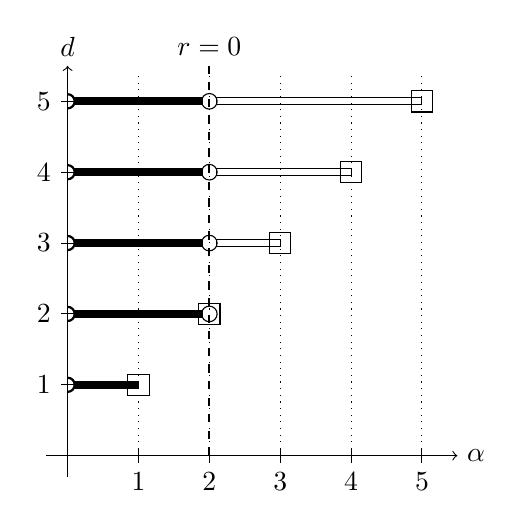
\begin{tikzpicture}[scale=0.9]
	\draw [thick,dashed] (2,0) -- (2,5.5) node [above] {$r=0$};
	\draw [->] (-0.3,0) -- (5.5,0) node [right] {$\alpha$};
	\draw [->] (0,-0.3) -- (0,5.5) node [above] {$d$};
	\foreach \x in {1,...,5}{
		\draw (\x,0.1)--++(0,-0.2) node [below] {$\x$};
		\draw (0.1,\x)--++(-0.2,0) node [left] {$\x$};
		\draw (\x,\x) + (-0.15,-0.15) rectangle +(0.15,0.15);
		\draw [thick] ([shift=(-90:0.1)]0,\x) arc (-90:90:0.1);
		\draw [thin, dotted] (\x,0) -- (\x, 5.4);
	}
	\filldraw (0, 1) + (0.1, -0.05) rectangle +(1,0.05);%\filldraw (1,1) circle (0.05);
	\filldraw (0, 2) + (0.1, -0.05) rectangle +(1.9,0.05);
	\filldraw (0, 3) + (0.1, -0.05) rectangle +(1.9,0.05);
	\filldraw (0, 4) + (0.1, -0.05) rectangle +(1.9,0.05);
	\filldraw (0, 5) + (0.1, -0.05) rectangle +(1.9,0.05);
	\draw (2,2) circle (0.11);
	\draw (2,3) circle (0.11);
	\draw (2,4) circle (0.11);
	\draw (2,5) circle (0.11);
	\draw (2, 3) + (0.1, -0.05) rectangle +(1,0.05);
	\draw (2, 4) + (0.1, -0.05) rectangle +(2,0.05);
	\draw (2, 5) + (0.1, -0.05) rectangle +(3,0.05);
	\end{tikzpicture}
	\hspace{2em}
	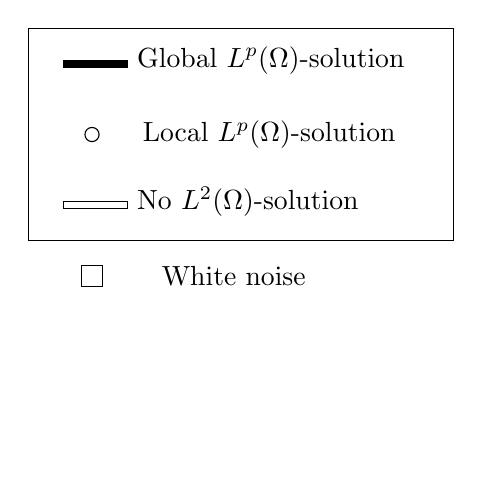
\begin{tikzpicture}[scale=0.9]
	\def\x{3}
	\draw (-0.4,-1.5+\x) rectangle +(6,3);
	\filldraw (0, 1+\x) + (0.1, -0.05) rectangle +(1,0.05) node [right] {Global $L^p(\Omega)$-solution};
	\draw (0.5,0+\x) circle (0.1); \node at (3,0+\x) {Local $L^p(\Omega)$-solution};
	\draw (0, -1+\x) + (0.1, -0.05) rectangle +(1,0.05) node [right] {No $L^2(\Omega)$-solution};
	\draw (0.5, 1) + (-0.15,-0.15) rectangle +(0.15,0.15); \node at (2.5,1) {White noise};
	\draw[white] (0,-1.5) circle (0.01);
	\end{tikzpicture}
	
	\caption{Solvability for the stochastic heat equation (i.e., $a=2$, $b=1$ and $r=0$) with $p\ge 2$.}
	\label{F:SHE}
\end{figure}

\begin{example}[SWE] \label{Eg:CriSWE}
	By setting $a=2$ and formally setting $b=2$ in \eqref{E:critical}, we obtain the following
	condition for the stochastic wave equation under which there only exists a local solution:
	\begin{align} \label{E:CrSWE}
	\alpha=3 + 2 r\le d \quad \text{and} \quad r\in[0,1/2].
	\end{align}
	We recall that results in Balan {\it et al} \cite{balan.chen.ea:22:exact} require $d\le 3$, and likewise,
	Assumption \ref{A:Nonnegative} and all known sufficient conditions for the nonnegativity of the
	fundamental solution (see Remark \ref{R:Nonnegative}) also require $d\le 3$ in case of $b\in
	(1,2)$. With this restriction, conditions \eqref{E:CrSWE} reduce to
	\begin{align*}
	\alpha=3=d \quad \text{and} \quad r=0,
	\end{align*}
	which says that at dimension $d=3$, when $\W$ is a white noise, there exists only a local
	$L^p(\Omega)$ solution for all $p\ge 2$. See Figure \ref{F:SWE} for an illustration. Moreover, one
	can check easily that the expression for the critical time $T_p$ in \eqref{E:Tp} in this case
	reduces to
	\begin{align} \label{E:TpCrSWE}
	T_p=  \frac{\nu^{3 / 2}}{2\theta (p-1) \sqrt{\mathcal{M}_{2,3}(\delta_0)}},  \quad p\ge 2,
	\end{align}
	which is identical to (1.12) ({\it ibid.}) when setting $\nu=2$. \bigskip
\end{example}

\begin{figure}[htb] % \label{F:SWE}
	\centering
	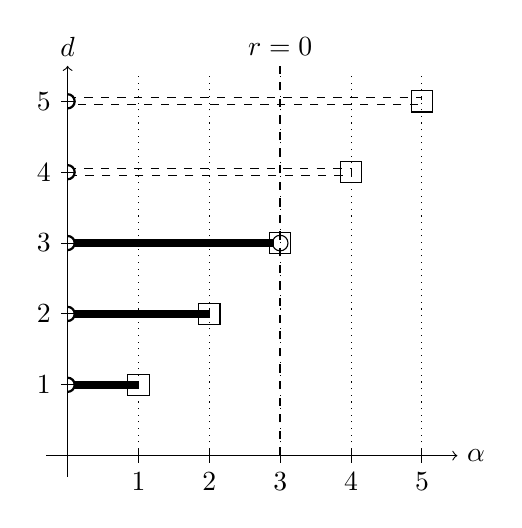
\begin{tikzpicture}[scale=0.9]
	\draw [thick,dashed] (3,0) -- (3,5.5) node [above] {$r=0$};
	\draw [->] (-0.3,0) -- (5.5,0) node [right] {$\alpha$};
	\draw [->] (0,-0.3) -- (0,5.5) node [above] {$d$};
	\foreach \x in {1,...,5}{
		\draw (\x,0.1)--++(0,-0.2) node [below] {$\x$};
		\draw (0.1,\x)--++(-0.2,0) node [left] {$\x$};
		\draw (\x,\x) + (-0.15,-0.15) rectangle +(0.15,0.15);
		\draw [thick] ([shift=(-90:0.1)]0,\x) arc (-90:90:0.1);
		\draw [thin, dotted] (\x,0) -- (\x, 5.4);
	}
	\filldraw (0, 1) + (0.1, -0.05) rectangle +(1,0.05);%\filldraw (1,1) circle (0.05);
	\filldraw (0, 2) + (0.1, -0.05) rectangle +(2,0.05);%\filldraw (2,2) circle (0.05);
	\filldraw (0, 3) + (0.1, -0.05) rectangle +(2.9,0.05);%\filldraw (3,3) circle (0.05);
	% \filldraw (0, 4) + (0.1, -0.05) rectangle +(2.9,0.05);
	% \filldraw (0, 5) + (0.1, -0.05) rectangle +(2.9,0.05);
	% \draw (2,2) circle (0.11);
	\draw (3,3) circle (0.11);
	% \draw (3,4) circle (0.11);
	% \draw (3,5) circle (0.11);
	% \draw (2, 3) + (0.1, -0.05) rectangle +(1,0.05);
	% \draw (2, 4) + (0.1, -0.05) rectangle +(2,0.05);
	\draw[dashed] (0, 5) + (0.1, -0.05) rectangle +(5,0.05);
	\draw[dashed] (0, 4) + (0.1, -0.05) rectangle +(4,0.05);
	\end{tikzpicture}
	\hspace{2em}
	\begin{tikzpicture}[scale=0.9]
	\def\x{3.2}
	% \draw (-0.4,-1.5+\x) rectangle +(6,3);
	\draw[dashed] (0, 1+\x) + (0.1, -0.05) rectangle +(1,0.05) node [right] {Unknown};
	% \draw (0.5,0+\x) circle (0.1); \node at (3,0+\x) {Local $L^p(\Omega)$-solution};
	% \draw (0, -1+\x) + (0.1, -0.05) rectangle +(1,0.05) node [right] {No $L^2(\Omega)$-solution};
	% \draw (0.5, 1) + (-0.15,-0.15) rectangle +(0.15,0.15); \node at (2.5,1) {White noise};
	\draw[white] (0,-1.5) circle (0.01);
	\end{tikzpicture}
	
	\caption{Solvability for the stochastic wave equation (i.e., $a=b=2$ and $r=0$). See Figure
		\ref{F:SHE} for an additional legend.}
	\label{F:SWE}
\end{figure}

\begin{example}[Fractional SPDEs with $r=\Ceil{b}-b$ and $a=2$] \label{Eg:FracSHE}
	For the fractional SDPEs with $b\ne 1$, many known works focus on the case when $r=\Ceil{b}-b$,
	where $\Ceil{b}$ is the ceiling function; see, e,g., \cite{chen:17:nonlinear, mijena.nane:15:space-time}. To
	facilitate the discussions here, we will only focus on the case when $a=2$. In particular, by
	setting $r=\Ceil{b}-b$ and $a=2$, conditions in \eqref{E:critical} become
	\begin{align} \label{E:CrFrSHE}
	\begin{cases}
	\displaystyle \alpha =\frac{2}{b} \le d \quad  \text{and} \quad b\in [1/2,1], \bigskip\\
	\displaystyle \alpha =\frac{6}{b} \le d \quad  \text{and} \quad b\in [3/2,2).
	\end{cases}
	\end{align}
	When $b=1$, we have $r=0$ and the fundamental solution is the standard heat kernel. Hence,
	Assumption \ref{A:Nonnegative} is satisfied for all $d\ge 1$. When $b<1$, sufficient conditions in
	Remark \ref{R:Nonnegative} guarantees Assumption \ref{A:Nonnegative} for all $d\ge 1$. However,
	when $b>1$ and $a=2$, from Remark \ref{R:Nonnegative} we see that the fundamental solution is
	nonnegative only for $d\le 3$. The solvability for this case is illustrated in Figure
	\ref{F:FracSHE} and the critical time $T_p$ in case of local solution (hence, only for the case
	when $b\in[1/2,1]$) is equal to
	\begin{align} \label{E:TpFracSHE}
	T_p = \dfrac{\nu^{\alpha/2}}{2 \theta (p-1) \mathcal{M}_{2,d}^{2-\alpha/2}}.
	\end{align}
\end{example}

\begin{figure}[htpb]% F:FracSHE
	\centering
	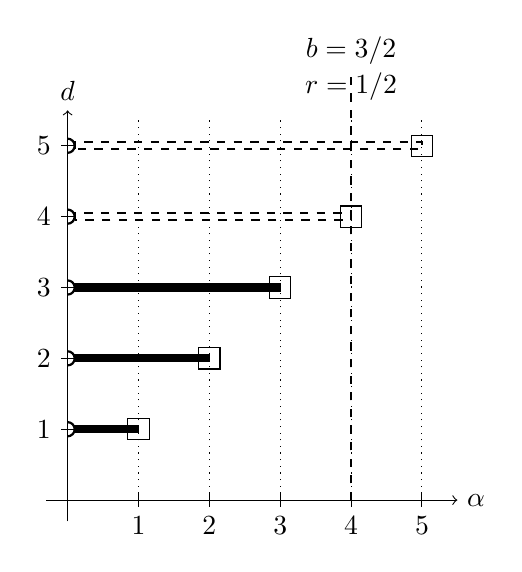
\begin{tikzpicture}[scale=0.9]
	\draw [thick,dashed] (4,0) -- (4,5.5) node [above] {$r=1/2$};
	\draw [thick,dashed] (4,0) -- (4,6) node [above] {$b=3/2$};
	\draw [->] (-0.3,0) -- (5.5,0) node [right] {$\alpha$};
	\draw [->] (0,-0.3) -- (0,5.5) node [above] {$d$};
	\foreach \x in {1,...,5}{
		\draw (\x,0.1)--++(0,-0.2) node [below] {$\x$};
		\draw (0.1,\x)--++(-0.2,0) node [left] {$\x$};
		\draw (\x,\x) + (-0.15,-0.15) rectangle +(0.15,0.15);
		\draw [thick] ([shift=(-90:0.1)]0,\x) arc (-90:90:0.1);
		\draw [thin, dotted] (\x,0) -- (\x, 5.4);
	}
	\filldraw (0, 1) + (0.1, -0.05) rectangle +(1,0.05);%\filldraw (1,1) circle (0.05);
	\filldraw (0, 2) + (0.1, -0.05) rectangle +(2,0.05);
	\filldraw (0, 3) + (0.1, -0.05) rectangle +(3,0.05);
	\draw[thick,dashed] (0, 4) + (0.1, -0.05) rectangle +(4,0.05);
	\draw[thick,dashed] (0, 5) + (0.1, -0.05) rectangle +(5,0.05);
	% \draw (2,2) circle (0.11);
	% \draw (2,3) circle (0.11);
	% \draw[thick,dotted] (4,4) circle (0.11);
	% \draw (4,5) circle (0.11);
	% \draw (2, 3) + (0.1, -0.05) rectangle +(1,0.05);
	% \draw (2, 4) + (0.1, -0.05) rectangle +(2,0.05);
	% \draw (2, 5) + (0.1, -0.05) rectangle +(3,0.05);
	\end{tikzpicture}
	\qquad \qquad
	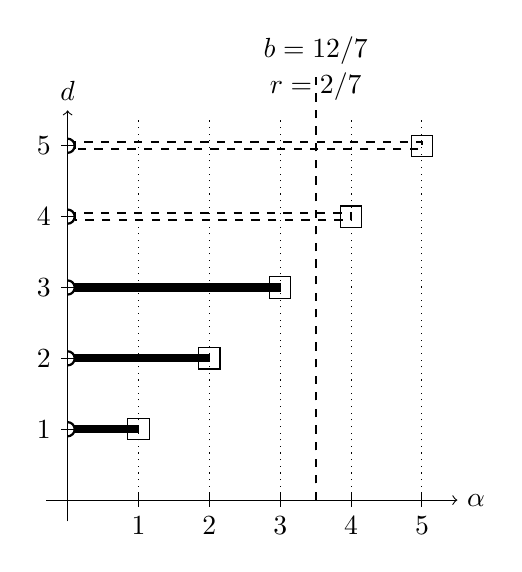
\begin{tikzpicture}[scale=0.9]
	\draw [thick,dashed] (3.5,0) -- (3.5,6) node [above] {$b=12/7$};
	\draw [thick,dashed] (3.5,0) -- (3.5,5.5) node [above] {$r=2/7$};
	\draw [->] (-0.3,0) -- (5.5,0) node [right] {$\alpha$};
	\draw [->] (0,-0.3) -- (0,5.5) node [above] {$d$};
	\foreach \x in {1,...,5}{
		\draw (\x,0.1)--++(0,-0.2) node [below] {$\x$};
		\draw (0.1,\x)--++(-0.2,0) node [left] {$\x$};
		\draw (\x,\x) + (-0.15,-0.15) rectangle +(0.15,0.15);
		\draw [thick] ([shift=(-90:0.1)]0,\x) arc (-90:90:0.1);
		\draw [thin, dotted] (\x,0) -- (\x, 5.4);
	}
	\filldraw (0, 1) + (0.1, -0.05) rectangle +(1,0.05);%\filldraw (1,1) circle (0.05);
	\filldraw (0, 2) + (0.1, -0.05) rectangle +(2,0.05);%\filldraw (2,2) circle (0.05);
	\filldraw (0, 3) + (0.1, -0.05) rectangle +(3,0.05);
	\draw[thick,dashed] (0, 4) + (0.1, -0.05) rectangle +(4,0.05);
	\draw[thick,dashed] (0, 5) + (0.1, -0.05) rectangle +(5,0.05);
	% \draw (2.5,2) circle (0.11);
	% \draw (2.5,3) circle (0.11);
	% \draw (2.5,4) circle (0.11);
	% \draw (2.5,5) circle (0.11);
	% \draw (2.5, 3) + (0.1, -0.05) rectangle +(0.5,0.05);
	% \draw (2.5, 4) + (0.1, -0.05) rectangle +(1.5,0.05);
	% \draw (2.5, 5) + (0.1, -0.05) rectangle +(2.5,0.05);
	\end{tikzpicture}
	\bigskip
	
	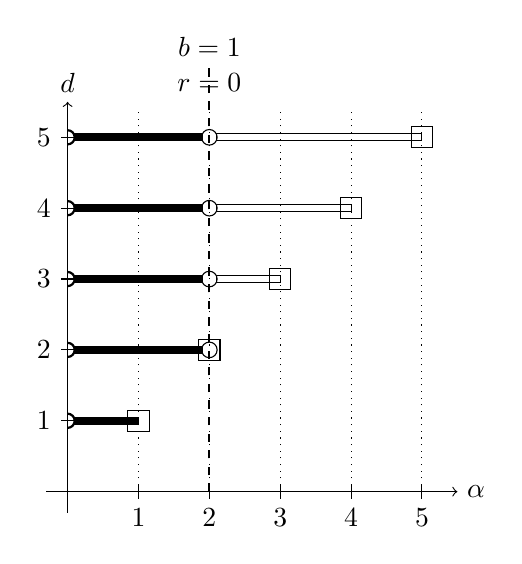
\begin{tikzpicture}[scale=0.9]
	\draw [thick,dashed] (2,0) -- (2,5.5) node [above] {$r=0$};
	\draw [thick,dashed] (2,0) -- (2,6) node [above] {$b=1$};
	\draw [->] (-0.3,0) -- (5.5,0) node [right] {$\alpha$};
	\draw [->] (0,-0.3) -- (0,5.5) node [above] {$d$};
	\foreach \x in {1,...,5}{
		\draw (\x,0.1)--++(0,-0.2) node [below] {$\x$};
		\draw (0.1,\x)--++(-0.2,0) node [left] {$\x$};
		\draw (\x,\x) + (-0.15,-0.15) rectangle +(0.15,0.15);
		\draw [thick] ([shift=(-90:0.1)]0,\x) arc (-90:90:0.1);
		\draw [thin, dotted] (\x,0) -- (\x, 5.4);
	}
	\filldraw (0, 1) + (0.1, -0.05) rectangle +(1,0.05);%\filldraw (1,1) circle (0.05);
	\filldraw (0, 2) + (0.1, -0.05) rectangle +(1.9,0.05);
	\filldraw (0, 3) + (0.1, -0.05) rectangle +(1.9,0.05);
	\filldraw (0, 4) + (0.1, -0.05) rectangle +(1.9,0.05);
	\filldraw (0, 5) + (0.1, -0.05) rectangle +(1.9,0.05);
	\draw (2,2) circle (0.11);
	\draw (2,3) circle (0.11);
	\draw (2,4) circle (0.11);
	\draw (2,5) circle (0.11);
	\draw (2, 3) + (0.1, -0.05) rectangle +(1,0.05);
	\draw (2, 4) + (0.1, -0.05) rectangle +(2,0.05);
	\draw (2, 5) + (0.1, -0.05) rectangle +(3,0.05);
	\end{tikzpicture}
	\qquad \qquad
	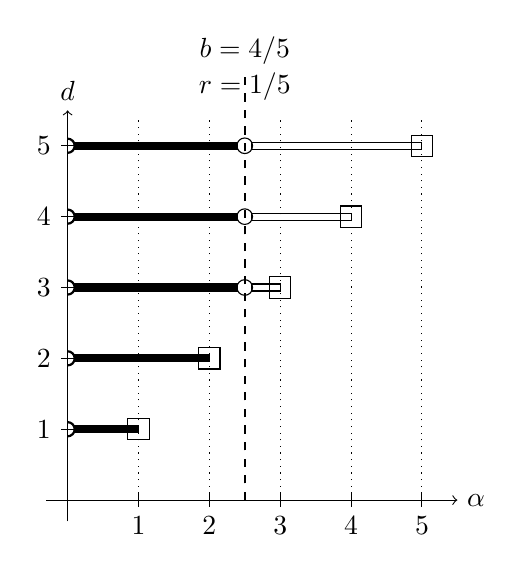
\begin{tikzpicture}[scale=0.9]
	\draw [thick,dashed] (2.5,0) -- (2.5,6) node [above] {$b=4/5$};
	\draw [thick,dashed] (2.5,0) -- (2.5,5.5) node [above] {$r=1/5$};
	\draw [->] (-0.3,0) -- (5.5,0) node [right] {$\alpha$};
	\draw [->] (0,-0.3) -- (0,5.5) node [above] {$d$};
	\foreach \x in {1,...,5}{
		\draw (\x,0.1)--++(0,-0.2) node [below] {$\x$};
		\draw (0.1,\x)--++(-0.2,0) node [left] {$\x$};
		\draw (\x,\x) + (-0.15,-0.15) rectangle +(0.15,0.15);
		\draw [thick] ([shift=(-90:0.1)]0,\x) arc (-90:90:0.1);
		\draw [thin, dotted] (\x,0) -- (\x, 5.4);
	}
	\filldraw (0, 1) + (0.1, -0.05) rectangle +(1,0.05);%\filldraw (1,1) circle (0.05);
	\filldraw (0, 2) + (0.1, -0.05) rectangle +(2,0.05);%\filldraw (2,2) circle (0.05);
	\filldraw (0, 3) + (0.1, -0.05) rectangle +(2.4,0.05);
	\filldraw (0, 4) + (0.1, -0.05) rectangle +(2.4,0.05);
	\filldraw (0, 5) + (0.1, -0.05) rectangle +(2.4,0.05);
	% \draw (2.5,2) circle (0.11);
	\draw (2.5,3) circle (0.11);
	\draw (2.5,4) circle (0.11);
	\draw (2.5,5) circle (0.11);
	\draw (2.5, 3) + (0.1, -0.05) rectangle +(0.5,0.05);
	\draw (2.5, 4) + (0.1, -0.05) rectangle +(1.5,0.05);
	\draw (2.5, 5) + (0.1, -0.05) rectangle +(2.5,0.05);
	\end{tikzpicture}
	\bigskip
	
	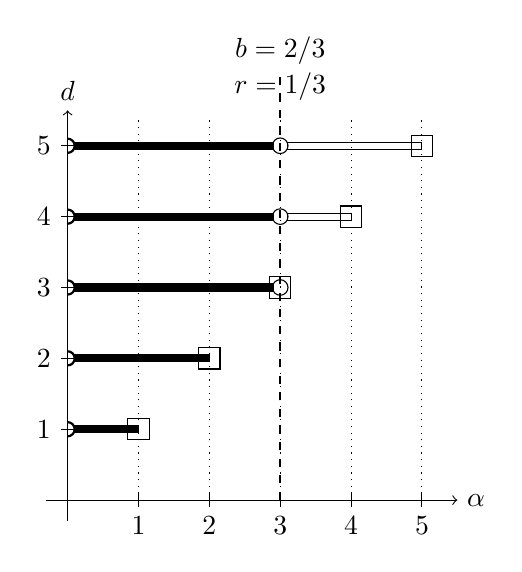
\begin{tikzpicture}[scale=0.9]
	\draw [thick,dashed] (3,0) -- (3,6) node [above] {$b=2/3$};
	\draw [thick,dashed] (3,0) -- (3,5.5) node [above] {$r=1/3$};
	\draw [->] (-0.3,0) -- (5.5,0) node [right] {$\alpha$};
	\draw [->] (0,-0.3) -- (0,5.5) node [above] {$d$};
	\foreach \x in {1,...,5}{
		\draw (\x,0.1)--++(0,-0.2) node [below] {$\x$};
		\draw (0.1,\x)--++(-0.2,0) node [left] {$\x$};
		\draw (\x,\x) + (-0.15,-0.15) rectangle +(0.15,0.15);
		\draw [thick] ([shift=(-90:0.1)]0,\x) arc (-90:90:0.1);
		\draw [thin, dotted] (\x,0) -- (\x, 5.4);
	}
	\filldraw (0, 1) + (0.1, -0.05) rectangle +(1,0.05);%\filldraw (1,1) circle (0.05);
	\filldraw (0, 2) + (0.1, -0.05) rectangle +(2,0.05);%\filldraw (2,2) circle (0.05);
	\filldraw (0, 3) + (0.1, -0.05) rectangle +(2.9,0.05);
	\filldraw (0, 4) + (0.1, -0.05) rectangle +(2.9,0.05);
	\filldraw (0, 5) + (0.1, -0.05) rectangle +(2.9,0.05);
	% \draw (2,2) circle (0.11);
	\draw (3,3) circle (0.11);
	\draw (3,4) circle (0.11);
	\draw (3,5) circle (0.11);
	% \draw (3, 3) + (0.1, -0.05) rectangle +(1,0.05);
	\draw (3, 4) + (0.1, -0.05) rectangle +(1,0.05);
	\draw (3, 5) + (0.1, -0.05) rectangle +(2,0.05);
	\end{tikzpicture}
	\qquad \qquad
	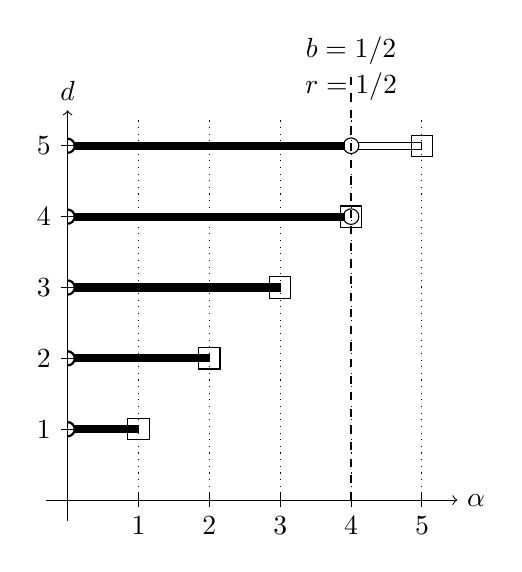
\begin{tikzpicture}[scale=0.9]
	\draw [thick,dashed] (4,0) -- (4,6) node [above] {$b=1/2$};
	\draw [thick,dashed] (4,0) -- (4,5.5) node [above] {$r=1/2$};
	\draw [->] (-0.3,0) -- (5.5,0) node [right] {$\alpha$};
	\draw [->] (0,-0.3) -- (0,5.5) node [above] {$d$};
	\foreach \x in {1,...,5}{
		\draw (\x,0.1)--++(0,-0.2) node [below] {$\x$};
		\draw (0.1,\x)--++(-0.2,0) node [left] {$\x$};
		\draw (\x,\x) + (-0.15,-0.15) rectangle +(0.15,0.15);
		\draw [thick] ([shift=(-90:0.1)]0,\x) arc (-90:90:0.1);
		\draw [thin, dotted] (\x,0) -- (\x, 5.4);
	}
	\filldraw (0, 1) + (0.1, -0.05) rectangle +(1,0.05);%\filldraw (1,1) circle (0.05);
	\filldraw (0, 2) + (0.1, -0.05) rectangle +(2,0.05);%\filldraw (2,2) circle (0.05);
	\filldraw (0, 3) + (0.1, -0.05) rectangle +(3,0.05);%\filldraw (3,3) circle (0.05);
	\filldraw (0, 4) + (0.1, -0.05) rectangle +(3.9,0.05);
	\filldraw (0, 5) + (0.1, -0.05) rectangle +(3.9,0.05);
	% \draw (2,2) circle (0.11);
	% \draw (2,3) circle (0.11);
	\draw (4,4) circle (0.11);
	\draw (4,5) circle (0.11);
	% \draw (2, 3) + (0.1, -0.05) rectangle +(1,0.05);
	% \draw (2, 4) + (0.1, -0.05) rectangle +(2,0.05);
	\draw (4, 5) + (0.1, -0.05) rectangle +(1,0.05);
	\end{tikzpicture}
	
	\caption{Solvability for the fractional SPDEs in case of $a=2$ and $r=\Ceil{b}-b$. See Figures
		\ref{F:SHE} and \ref{F:SWE} for the legend.}
	\label{F:FracSHE}
\end{figure}

\begin{example}[Fractional SPDEs with $r=0$ and $a=2$] \label{Eg:FracSHE0}
	In this example, we study the special case of the fractional SPDEs when $r=0$. The choice of $r=0$
	has been used in, e.g., \cite{chen.hu.ea:17:space-time}.  We will only consider the case $a=2$ for simplicity. Now
	by setting $r=0$ and $a=2$ and restricting $b\le 1$, conditions in \eqref{E:critical} become
	\begin{align} \label{E:CrFrSHE2}
	\alpha =4- \frac{2}{b} \le d \quad  \text{and} \quad b\in (0,1].
	\end{align}
	As discussed in Example \ref{Eg:FracSHE}, Assumption \ref{A:Nonnegative} is satisfied for all
	$d\ge 1$ when $b\le 1$ but only for $d\le 3$ when $b>1$. The solvability for this case is
	illustrated in Figure \ref{F:FracSHE0} with $T_p$ given in \eqref{E:TpFracSHE}. In particular, for
	the example in the second figure in Figure \ref{F:FracSHE0}, namely, when $b=2/3$ and
	$\alpha=d=1$, the white noise driven SHE has a local solution with
	\begin{align}
	T_p= \frac{2^{5/2}\sqrt{\nu}}{3(p-1)\theta}, \qquad \text{for all $p\ge 2$,}
	\end{align}
	where we have applied \eqref{E:TpFracSHE} and the relation \eqref{E:Mdelta1d}.
\end{example}

More examples regarding the solvability can be studied in a similar way, which are left to the
interested readers.

\begin{figure}[htpb]% F:FracSHE0
	\centering
	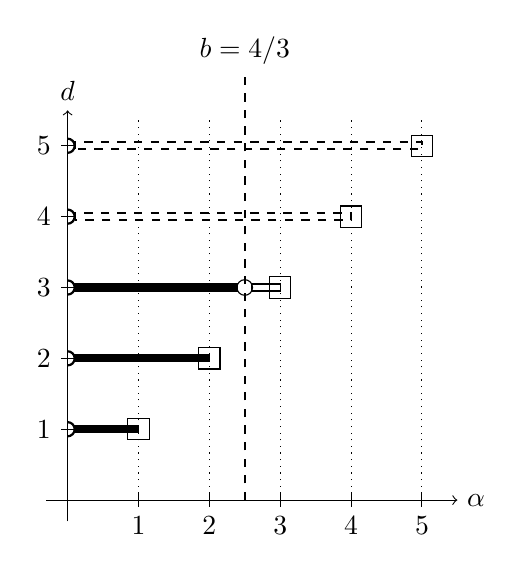
\begin{tikzpicture}[scale=0.9]
	% \draw [thick,dashed] (2,0) -- (2,5.5) node [above] {$r=0$};
	\draw [thick,dashed] (2.5,0) -- (2.5,6) node [above] {$b=4/3$};
	\draw [->] (-0.3,0) -- (5.5,0) node [right] {$\alpha$};
	\draw [->] (0,-0.3) -- (0,5.5) node [above] {$d$};
	\foreach \x in {1,...,5}{
		\draw (\x,0.1)--++(0,-0.2) node [below] {$\x$};
		\draw (0.1,\x)--++(-0.2,0) node [left] {$\x$};
		\draw (\x,\x) + (-0.15,-0.15) rectangle +(0.15,0.15);
		\draw [thick] ([shift=(-90:0.1)]0,\x) arc (-90:90:0.1);
		\draw [thin, dotted] (\x,0) -- (\x, 5.4);
	}
	\filldraw (0, 1) + (0.1, -0.05) rectangle +(1,0.05);%\filldraw (1,1) circle (0.05);
	\filldraw (0, 2) + (0.1, -0.05) rectangle +(2,0.05);
	\filldraw (0, 3) + (0.1, -0.05) rectangle +(2.4,0.05);
	\draw[thick,dashed] (0, 4) + (0.1, -0.05) rectangle +(4,0.05);
	\draw[thick,dashed] (0, 5) + (0.1, -0.05) rectangle +(5,0.05);
	\draw (2.5,3) circle (0.11);
	% \draw (2.5,4) circle (0.11);
	% \draw (2.5,5) circle (0.11);
	\draw (2.5,3) + (0.1, -0.05) rectangle +(0.5,0.05);
	% \draw (2.5,4) + (0.1, -0.05) rectangle +(1.5,0.05);
	% \draw (2.5,5) + (0.1, -0.05) rectangle +(2.5,0.05);
	\end{tikzpicture}
	\qquad \qquad
	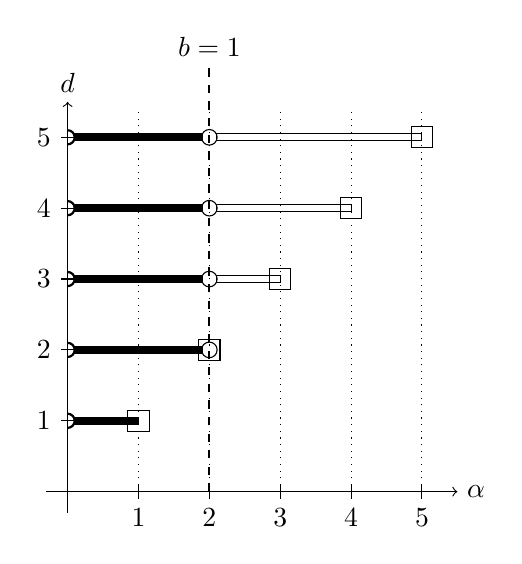
\begin{tikzpicture}[scale=0.9]
	% \draw [thick,dashed] (2,0) -- (2,5.5) node [above] {$r=0$};
	\draw [thick,dashed] (2,0) -- (2,6) node [above] {$b=1$};
	\draw [->] (-0.3,0) -- (5.5,0) node [right] {$\alpha$};
	\draw [->] (0,-0.3) -- (0,5.5) node [above] {$d$};
	\foreach \x in {1,...,5}{
		\draw (\x,0.1)--++(0,-0.2) node [below] {$\x$};
		\draw (0.1,\x)--++(-0.2,0) node [left] {$\x$};
		\draw (\x,\x) + (-0.15,-0.15) rectangle +(0.15,0.15);
		\draw [thick] ([shift=(-90:0.1)]0,\x) arc (-90:90:0.1);
		\draw [thin, dotted] (\x,0) -- (\x, 5.4);
	}
	\filldraw (0, 1) + (0.1, -0.05) rectangle +(1,0.05);%\filldraw (1,1) circle (0.05);
	\filldraw (0, 2) + (0.1, -0.05) rectangle +(1.9,0.05);
	\filldraw (0, 3) + (0.1, -0.05) rectangle +(1.9,0.05);
	\filldraw (0, 4) + (0.1, -0.05) rectangle +(1.9,0.05);
	\filldraw (0, 5) + (0.1, -0.05) rectangle +(1.9,0.05);
	\draw (2,2) circle (0.11);
	\draw (2,3) circle (0.11);
	\draw (2,4) circle (0.11);
	\draw (2,5) circle (0.11);
	\draw (2, 3) + (0.1, -0.05) rectangle +(1,0.05);
	\draw (2, 4) + (0.1, -0.05) rectangle +(2,0.05);
	\draw (2, 5) + (0.1, -0.05) rectangle +(3,0.05);
	\end{tikzpicture}
	
	\bigskip
	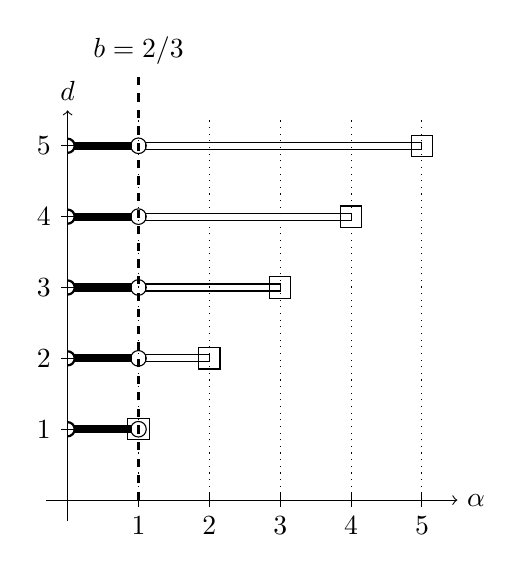
\begin{tikzpicture}[scale=0.9]
	\draw [thick,dashed] (1,0) -- (1,6) node [above] {$b=2/3$};
	% \draw [thick,dashed] (0.5,0) -- (0.5,5.5) node [above] {$r=0$};
	\draw [->] (-0.3,0) -- (5.5,0) node [right] {$\alpha$};
	\draw [->] (0,-0.3) -- (0,5.5) node [above] {$d$};
	\foreach \x in {1,...,5}{
		\draw (\x,0.1)--++(0,-0.2) node [below] {$\x$};
		\draw (0.1,\x)--++(-0.2,0) node [left] {$\x$};
		\draw (\x,\x) + (-0.15,-0.15) rectangle +(0.15,0.15);
		\draw [thick] ([shift=(-90:0.1)]0,\x) arc (-90:90:0.1);
		\draw [thin, dotted] (\x,0) -- (\x, 5.4);
	}
	\filldraw (0, 1) + (0.1, -0.05) rectangle +(0.9,0.05);%\filldraw (1,1) circle (0.05);
	\filldraw (0, 2) + (0.1, -0.05) rectangle +(0.9,0.05);%\filldraw (2,2) circle (0.05);
	\filldraw (0, 3) + (0.1, -0.05) rectangle +(0.9,0.05);
	\filldraw (0, 4) + (0.1, -0.05) rectangle +(0.9,0.05);
	\filldraw (0, 5) + (0.1, -0.05) rectangle +(0.9,0.05);
	% \draw (2.5,2) circle (0.11);
	\draw (1,1) circle (0.11);
	\draw (1,2) circle (0.11);
	\draw (1,3) circle (0.11);
	\draw (1,4) circle (0.11);
	\draw (1,5) circle (0.11);
	% \draw (1, 1) + (0.1, -0.05) rectangle +(0.5,0.05);
	\draw (1, 2) + (0.1, -0.05) rectangle +(1,0.05);
	\draw (1, 3) + (0.1, -0.05) rectangle +(2,0.05);
	\draw (1, 4) + (0.1, -0.05) rectangle +(3,0.05);
	\draw (1, 5) + (0.1, -0.05) rectangle +(4,0.05);
	\end{tikzpicture}
	\qquad \qquad
	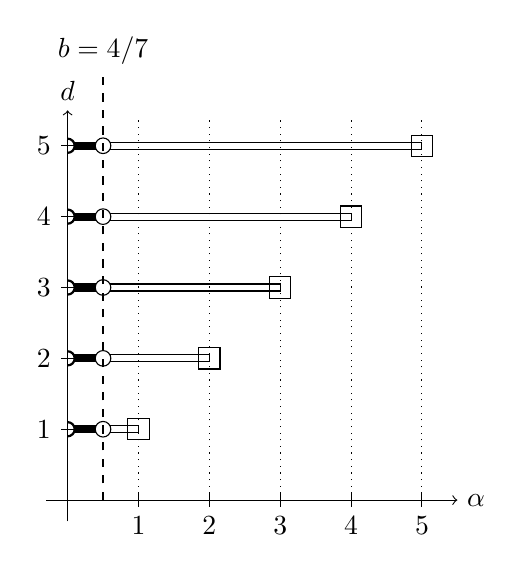
\begin{tikzpicture}[scale=0.9]
	\draw [thick,dashed] (0.5,0) -- (0.5,6) node [above] {$b=4/7$};
	% \draw [thick,dashed] (0.5,0) -- (0.5,5.5) node [above] {$r=0$};
	\draw [->] (-0.3,0) -- (5.5,0) node [right] {$\alpha$};
	\draw [->] (0,-0.3) -- (0,5.5) node [above] {$d$};
	\foreach \x in {1,...,5}{
		\draw (\x,0.1)--++(0,-0.2) node [below] {$\x$};
		\draw (0.1,\x)--++(-0.2,0) node [left] {$\x$};
		\draw (\x,\x) + (-0.15,-0.15) rectangle +(0.15,0.15);
		\draw [thick] ([shift=(-90:0.1)]0,\x) arc (-90:90:0.1);
		\draw [thin, dotted] (\x,0) -- (\x, 5.4);
	}
	\filldraw (0, 1) + (0.1, -0.05) rectangle +(0.4,0.05);%\filldraw (1,1) circle (0.05);
	\filldraw (0, 2) + (0.1, -0.05) rectangle +(0.4,0.05);%\filldraw (2,2) circle (0.05);
	\filldraw (0, 3) + (0.1, -0.05) rectangle +(0.4,0.05);
	\filldraw (0, 4) + (0.1, -0.05) rectangle +(0.4,0.05);
	\filldraw (0, 5) + (0.1, -0.05) rectangle +(0.4,0.05);
	% \draw (2.5,2) circle (0.11);
	\draw (0.5,1) circle (0.11);
	\draw (0.5,2) circle (0.11);
	\draw (0.5,3) circle (0.11);
	\draw (0.5,4) circle (0.11);
	\draw (0.5,5) circle (0.11);
	\draw (0.5, 1) + (0.1, -0.05) rectangle +(0.5,0.05);
	\draw (0.5, 2) + (0.1, -0.05) rectangle +(1.5,0.05);
	\draw (0.5, 3) + (0.1, -0.05) rectangle +(2.5,0.05);
	\draw (0.5, 4) + (0.1, -0.05) rectangle +(3.5,0.05);
	\draw (0.5, 5) + (0.1, -0.05) rectangle +(4.5,0.05);
	\end{tikzpicture}
	\caption{Solvability for the fractional SPDEs in case of $a=2$ and $r=0$. See Figures \ref{F:SHE} and \ref{F:SWE} for the legend.}
	\label{F:FracSHE0}
\end{figure}

\begin{example}[SHE with fractional Laplacian] \label{Eg:StableSHE}
	The stochastic heat equation with fractional Laplacian (i.e., the case when $b=1$, $r=0$ and $a\in
	(0,2]$) has been widely studied in the literature, but possibly with different noises. In this
	case, the fundamental solutions are transition densities for the alpha-stable jump processes,
	which are necessarily to be nonnegative. This is also consistent with the sufficient conditions
	for nonnegativity in Remark \ref{R:Nonnegative}. By setting $b=1$ and $r=0$ in \eqref{E:critical},
	we have the following condition:
	\begin{align*}
	\alpha = a \le d
	\end{align*}
	The solvability for this case is illustrated in Figure \ref{F:Stable}.
\end{example}

\begin{figure}[htpb]% F:Stable
	\centering
	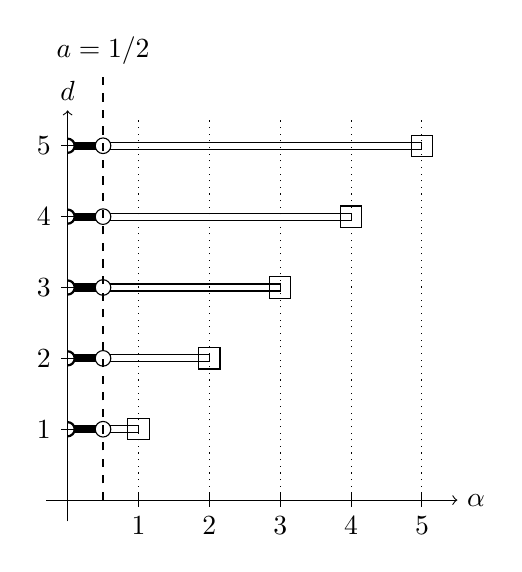
\begin{tikzpicture}[scale=0.9]
	% \draw [thick,dashed] (2,0) -- (2,5.5) node [above] {$r=0$};
	\draw [thick,dashed] (0.5,0) -- (0.5,6) node [above] {$a=1/2$};
	\draw [->] (-0.3,0) -- (5.5,0) node [right] {$\alpha$};
	\draw [->] (0,-0.3) -- (0,5.5) node [above] {$d$};
	\foreach \x in {1,...,5}{
		\draw (\x,0.1)--++(0,-0.2) node [below] {$\x$};
		\draw (0.1,\x)--++(-0.2,0) node [left] {$\x$};
		\draw (\x,\x) + (-0.15,-0.15) rectangle +(0.15,0.15);
		\draw [thick] ([shift=(-90:0.1)]0,\x) arc (-90:90:0.1);
		\draw [thin, dotted] (\x,0) -- (\x, 5.4);
	}
	\filldraw (0, 1) + (0.1, -0.05) rectangle +(0.4,0.05);
	\filldraw (0, 2) + (0.1, -0.05) rectangle +(0.4,0.05);
	\filldraw (0, 3) + (0.1, -0.05) rectangle +(0.4,0.05);
	\filldraw (0, 4) + (0.1, -0.05) rectangle +(0.4,0.05);
	\filldraw (0, 5) + (0.1, -0.05) rectangle +(0.4,0.05);
	\draw (0.5,1) circle (0.11);
	\draw (0.5,2) circle (0.11);
	\draw (0.5,3) circle (0.11);
	\draw (0.5,4) circle (0.11);
	\draw (0.5,5) circle (0.11);
	\draw (0.5,1) + (0.1, -0.05) rectangle +(0.5,0.05);
	\draw (0.5,2) + (0.1, -0.05) rectangle +(1.5,0.05);
	\draw (0.5,3) + (0.1, -0.05) rectangle +(2.5,0.05);
	\draw (0.5,4) + (0.1, -0.05) rectangle +(3.5,0.05);
	\draw (0.5,5) + (0.1, -0.05) rectangle +(4.5,0.05);
	\end{tikzpicture}
	\qquad \qquad
	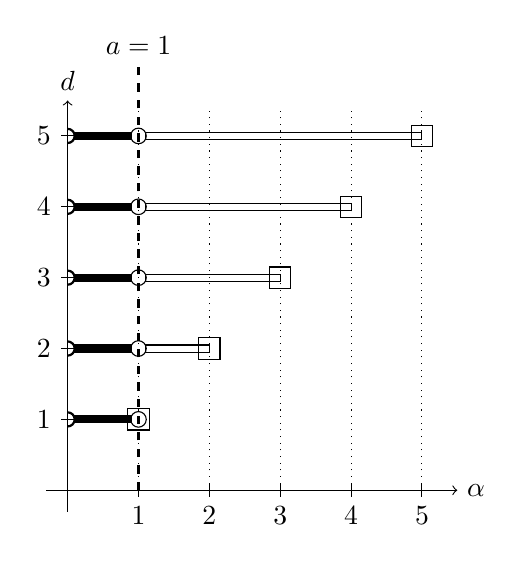
\begin{tikzpicture}[scale=0.9]
	% \draw [thick,dashed] (2,0) -- (2,5.5) node [above] {$r=0$};
	\draw [thick,dashed] (1,0) -- (1,6) node [above] {$a=1$};
	\draw [->] (-0.3,0) -- (5.5,0) node [right] {$\alpha$};
	\draw [->] (0,-0.3) -- (0,5.5) node [above] {$d$};
	\foreach \x in {1,...,5}{
		\draw (\x,0.1)--++(0,-0.2) node [below] {$\x$};
		\draw (0.1,\x)--++(-0.2,0) node [left] {$\x$};
		\draw (\x,\x) + (-0.15,-0.15) rectangle +(0.15,0.15);
		\draw [thick] ([shift=(-90:0.1)]0,\x) arc (-90:90:0.1);
		\draw [thin, dotted] (\x,0) -- (\x, 5.4);
	}
	\filldraw (0, 1) + (0.1, -0.05) rectangle +(0.9,0.05);%\filldraw (1,1) circle (0.05);
	\filldraw (0, 2) + (0.1, -0.05) rectangle +(0.9,0.05);
	\filldraw (0, 3) + (0.1, -0.05) rectangle +(0.9,0.05);
	\filldraw (0, 4) + (0.1, -0.05) rectangle +(0.9,0.05);
	\filldraw (0, 5) + (0.1, -0.05) rectangle +(0.9,0.05);
	\draw (1,1) circle (0.11);
	\draw (1,2) circle (0.11);
	\draw (1,3) circle (0.11);
	\draw (1,4) circle (0.11);
	\draw (1,5) circle (0.11);
	\draw (1, 2) + (0.1, -0.05) rectangle +(1,0.05);
	\draw (1, 3) + (0.1, -0.05) rectangle +(2,0.05);
	\draw (1, 4) + (0.1, -0.05) rectangle +(3,0.05);
	\draw (1, 5) + (0.1, -0.05) rectangle +(4,0.05);
	\end{tikzpicture}
	
	\bigskip
	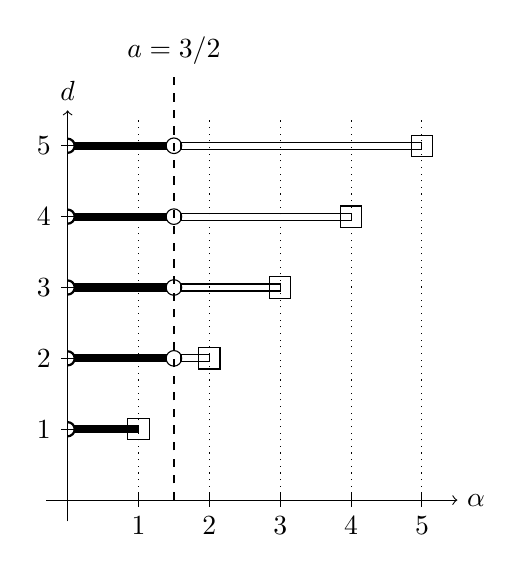
\begin{tikzpicture}[scale=0.9]
	\draw [thick,dashed] (1.5,0) -- (1.5,6) node [above] {$a=3/2$};
	% \draw [thick,dashed] (0.5,0) -- (0.5,5.5) node [above] {$r=0$};
	\draw [->] (-0.3,0) -- (5.5,0) node [right] {$\alpha$};
	\draw [->] (0,-0.3) -- (0,5.5) node [above] {$d$};
	\foreach \x in {1,...,5}{
		\draw (\x,0.1)--++(0,-0.2) node [below] {$\x$};
		\draw (0.1,\x)--++(-0.2,0) node [left] {$\x$};
		\draw (\x,\x) + (-0.15,-0.15) rectangle +(0.15,0.15);
		\draw [thick] ([shift=(-90:0.1)]0,\x) arc (-90:90:0.1);
		\draw [thin, dotted] (\x,0) -- (\x, 5.4);
	}
	\filldraw (0, 1) + (0.1, -0.05) rectangle +(1,0.05);%\filldraw (1,1) circle (0.05);
	\filldraw (0, 2) + (0.1, -0.05) rectangle +(1.4,0.05);%\filldraw (2,2) circle (0.05);
	\filldraw (0, 3) + (0.1, -0.05) rectangle +(1.4,0.05);
	\filldraw (0, 4) + (0.1, -0.05) rectangle +(1.4,0.05);
	\filldraw (0, 5) + (0.1, -0.05) rectangle +(1.4,0.05);
	\draw (1.5,2) circle (0.11);
	\draw (1.5,3) circle (0.11);
	\draw (1.5,4) circle (0.11);
	\draw (1.5,5) circle (0.11);
	\draw (1.5, 2) + (0.1, -0.05) rectangle +(0.5,0.05);
	\draw (1.5, 3) + (0.1, -0.05) rectangle +(1.5,0.05);
	\draw (1.5, 4) + (0.1, -0.05) rectangle +(2.5,0.05);
	\draw (1.5, 5) + (0.1, -0.05) rectangle +(3.5,0.05);
	\end{tikzpicture}
	\qquad \qquad
	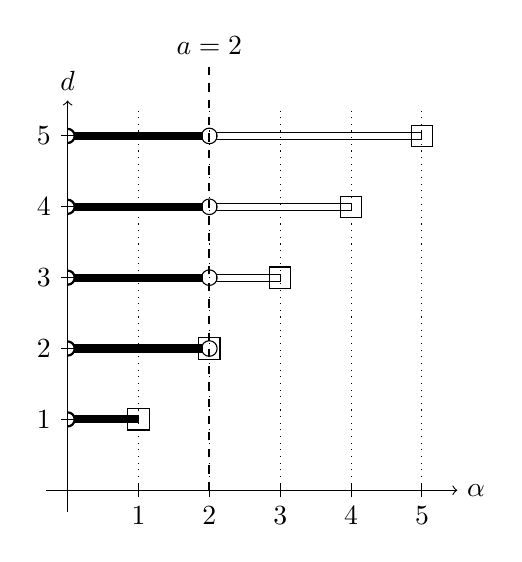
\begin{tikzpicture}[scale=0.9]
	\draw [thick,dashed] (2,0) -- (2,6) node [above] {$a=2$};
	% \draw [thick,dashed] (0.5,0) -- (0.5,5.5) node [above] {$r=0$};
	\draw [->] (-0.3,0) -- (5.5,0) node [right] {$\alpha$};
	\draw [->] (0,-0.3) -- (0,5.5) node [above] {$d$};
	\foreach \x in {1,...,5}{
		\draw (\x,0.1)--++(0,-0.2) node [below] {$\x$};
		\draw (0.1,\x)--++(-0.2,0) node [left] {$\x$};
		\draw (\x,\x) + (-0.15,-0.15) rectangle +(0.15,0.15);
		\draw [thick] ([shift=(-90:0.1)]0,\x) arc (-90:90:0.1);
		\draw [thin, dotted] (\x,0) -- (\x, 5.4);
	}
	\filldraw (0, 1) + (0.1, -0.05) rectangle +(1,0.05);%\filldraw (1,1) circle (0.05);
	\filldraw (0, 2) + (0.1, -0.05) rectangle +(1.9,0.05);%\filldraw (2,2) circle (0.05);
	\filldraw (0, 3) + (0.1, -0.05) rectangle +(1.9,0.05);
	\filldraw (0, 4) + (0.1, -0.05) rectangle +(1.9,0.05);
	\filldraw (0, 5) + (0.1, -0.05) rectangle +(1.9,0.05);
	\draw (2,2) circle (0.11);
	\draw (2,3) circle (0.11);
	\draw (2,4) circle (0.11);
	\draw (2,5) circle (0.11);
	\draw (2, 3) + (0.1, -0.05) rectangle +(1,0.05);
	\draw (2, 4) + (0.1, -0.05) rectangle +(2,0.05);
	\draw (2, 5) + (0.1, -0.05) rectangle +(3,0.05);
	\end{tikzpicture}
	\caption{Solvability for the stochastic heat equation with fractional Laplacian, i.e, the case when
		$b=1$ and $r=0$. See Figures \ref{F:SHE} and \ref{F:SWE} for the legend.}
	\label{F:Stable}
\end{figure}

\subsection{Examples on asymptotics} \label{SS:EgAsym}

In this part, we list several examples for the asymptotics when global solutions exist. In
particular, we will show that the asymptotics in \eqref{E:momentasym} interpolates the corresponding
results for both stochastic wave and heat equations.

\begin{example}[Asymptotics for SWE] \label{Eg:AsymSWE}
	Even though our results requires $b$ to be strictly less than $2$, but by formally setting
	\begin{align*}
	a = b = \nu = 2 \quad \text{and} \quad r = 0,
	\end{align*}
	we have that
	\begin{align*}
	\beta = \frac{4-\alpha}{3-\alpha} \quad \text{and} \quad
	t_p   = (p-1)^{1/(4-\alpha)} t,
	\end{align*}
	and results in \eqref{E:momentasym}, \eqref{E:momentasym-t}, and \eqref{E:momentasym-p} recover
	the corresponding results for the stochastic wave equation, namely, (1.9), (1.10), and (1.11) of \cite{balan.chen.ea:22:exact}, respectively.  Due to the importance of white noise and for the future references,
	here we list two special cases regarding white noise:\\
	
	\noindent(1) The SWE with white noise in $\R$: By further setting $d=\alpha=1$, we see that
	\begin{align} \label{E:AsymSWE-1d}
	% =p(p-1)^{1/2}\frac{2^{3/2}\sqrt{\theta} \mathcal{M}_2^{3/4}(\delta_0)}{ 2^{3/2}\nu^{1/4}}
	\lim_{t \to \infty} \frac{\log \E\left[|u(t,x)|^p\right]}{t^{3/2}} =  \frac{p(p-1)^{1/2}\sqrt{\theta}}{3 (2\nu)^{1/4}}
	\quad \text{and} \quad
	\lim_{p \to \infty} \frac{\log \E\left[|u(t,x)|^p\right]}{p^{3/2}} = \frac{t^{3/2}\sqrt{\theta}}{3 (2\nu)^{1/4}},
	\end{align}
	where we have applied \eqref{E:Mdelta1d}.\\
	
	\noindent(2) The SWE with white noise in $\R^2$: Similarly, by setting $d=\alpha=2$, we see that
	\begin{align} \label{E:AsymSWE-2d}
	% =p(p-1)^{1/2}\frac{2^{3/2}\sqrt{\theta} \mathcal{M}_2^{3/4}(\delta_0)}{ 2^{3/2}\nu^{1/4}}
	\lim_{t \to \infty} \frac{\log \E\left[|u(t,x)|^p\right]}{t^2} = \frac{p(p-1)\theta\mathcal{M}_{2,2}(\delta_0)}{2\nu}
	\quad \text{and} \quad
	\lim_{p \to \infty} \frac{\log \E\left[|u(t,x)|^p\right]}{p^2} = \frac{t^2\theta\mathcal{M}_{2,2}(\delta_0)}{2\nu}.
	\end{align}
\end{example}

\begin{example}[Asymptotics for SHE]
	\label{Eg:AsymSHE} As for the stochastic heat equation case, by setting
	\begin{align*}
	a = 2,\quad b= \nu = 1 \quad \text{and} \quad r = 0,
	\end{align*}
	we have that
	\begin{align*}
	\beta = \frac{4-\alpha}{2-\alpha} \quad \text{and} \quad
	t_p=(p-1)^{2/(4-\alpha)}t,
	\end{align*}
	and results in \eqref{E:momentasym} and \eqref{E:momentasym-t} recover the corresponding
	conjectured results for SHE, namely, (1.16) and (1.17) of Balan {\it et al} \cite{balan.chen.ea:22:exact},
	respectively, which are equivalent to Theorem 1.1 and 1.2 of X. Chen \cite{chen:17:moment} when
	setting $\alpha_0=0$ and using \cite[Lemma A.2]{chen.hu.ea:15:exponential} to rewrite the constant $\mathcal{E}$ in \cite{chen:17:moment} in terms of $\mathcal{M}_a$. Due to the importance of the white noise case, we
	list the corresponding asymptotics here. When $\alpha=d=1$,
	\begin{align} \label{E:AsymSHE1d}
	\lim_{t \to \infty} \frac{\log \E\left(|u(t,x)|^p\right)}{t^3} = \frac{p(p-1)^2\theta^2}{24\nu}
	\quad \text{and} \quad
	\lim_{p \to \infty} \frac{\log \E\left(|u(t,x)|^p\right)}{p^3} = \frac{t^3\theta^2}{24\nu},
	\end{align}
	where we have applied \eqref{E:Mdelta1d}. Note that some upper and lower bounds for the first
	limit in \eqref{E:AsymSHE1d} in case of $p=2$ were earlier obtained by Hu \cite[part 1) of Theorem
	4.1]{hu:02:chaos}.
\end{example}

\begin{example}[Asymptotics for SHE with fractional Laplacian] \label{Eg:AsymStable}
	In this example we restrict ourselves to the case when $b=1$, $a\in (0,2]$, $\alpha < d$, and
	$r=0$, which is the 1-dimensional SHE with fractional Laplace. With this set up we have
	\begin{align*}
	\beta = \frac{2a-\alpha}{a-\alpha} \qquad \text{and} \qquad t_p = (p-1)^{\frac{a}{2a-\alpha}} t,
	\end{align*}
	and by Corollary \ref{C:Lim},
	\begin{align} \label{E:AsymStable-t}
	\lim_{t \to \infty} \frac{\log \E\left(|u(t,x)|^p\right)}{t^{\frac{2a-\alpha}{a-\alpha} }} =
	p (p-1)^{\frac{a}{a-\alpha}} \left( \frac{1}{2} \right)\left( \frac{2a}{2a-\alpha} \right)^{\frac{2a-\alpha}{a-\alpha}}
	\left[ \theta \nu^{-\alpha/a} \mathcal{M}_{a,d}^{\frac{2a-\alpha}{a}} \right]^{ \frac{a}{a-\alpha} } \left(\frac{a-\alpha}{a}\right)
	\end{align}
	and
	\begin{align} \label{E:AsymStable-p}
	\lim_{p \to \infty} \frac{\log \E\left(|u(t,x)|^p\right)}{p^{\frac{2a-\alpha}{a-\alpha} }} =
	t^{\frac{2a-\alpha}{a-\alpha}}
	\left( \frac{1}{2} \right)\left( \frac{2a}{2a-\alpha} \right)^{\frac{2a-\alpha}{a-\alpha}}
	\left[ \theta \nu^{-\alpha/a} \mathcal{M}_{a,d}^{\frac{2a-\alpha}{a}} \right]^{ \frac{a}{a-\alpha} } \left(\frac{a-\alpha}{a}\right).
	\end{align}
	this setup has been studied in \cite{chen.hu.ea:18:temporal} for the case of a time-dependent noise where the
	covariance function is given by
	\begin{align*}
	\mathbb{E}[\dot{W}(r,x)\dot{W}(s,y)] = |r-s|^{-\alpha_0}\gamma(x-y)
	\end{align*}
	and $\gamma(x)$ is defined to be either of the following:
	\begin{align} \label{E:gammaHu}
	\gamma(x) := \begin{cases}
	|x|^{-\alpha}                  & \text{where } \alpha \in (0,d)\: \text{ or} \\
	\prod_{j=1}^d |x_j|^{\alpha_j} & \text{where } \alpha_j \in (0,1).
	\end{cases}
	\end{align}
	They proved that for $\alpha < \min\{a,d\}$ and let $p \ge 2$,
	\begin{equation}\label{E:AsymVar}
	\lim_{t\to\infty} t^{-\frac{2a - \alpha - \alpha\alpha_0}{a-\alpha}}\log\mathbb{E}[|u(t,x)|^p]
	= p(p-1)^{\frac{a}{a-\alpha}}\textbf{M}(a,\alpha_0,d,\gamma),
	\end{equation}
	where the variational constant is given by
	\begin{align*}
	\textbf{M}(a,\alpha_0,d,\gamma) = \sup_{g \in \mathcal{A}_{a,d}} \bigg\{ \frac{1}{2} \int_0^1\int_0^1 \int_{\R^{2d}}
	& \frac{\gamma(x-y)}{|r-s|^{\alpha_0}}g^2(s,x)g^2(r,y)  \ud x \ud y \ud r \ud s \\
	& - (2\pi)^{-d} \int_0^1 \int_{\R^d} |x|^a |\mathcal{F}g(s,\xi)|^2 \ud \xi \ud s \bigg\}
	\end{align*}
	with\footnote{Note that the Fourier transform is defined differently in \cite{chen.hu.ea:18:temporal}.}
	\begin{align*}
	\mathcal{A}_{a,d} := \left\{ g(s,x) : \int_{\R^d} g^2(s,x) \ud x = 1, \forall s \in [0,1] \text{ and }
	(2\pi)^{-d} \int_0^1 \int_{\R^d} |x|^a |\mathcal{F}g(s,\xi)|^2 \ud \xi \ud s < \infty \right\}.
	\end{align*}
	By setting $\alpha_0=0$ and letting $g(s,x)=g(x) \in \mathcal{F}_a$ be independent in $s$, which
	is the time-independent setup, then Equation \eqref{E:AsymStable-t} and Lemma \ref{L:EvsM}
	together recover \eqref{E:AsymVar}. Indeed, by observing \eqref{E:VarConstE} and \eqref{E:EvsM},
	we see that
	\begin{align}
	\textbf{M}(a,\alpha_0,d,\gamma)
	& = \mathbf{E}_{a,d}\left(\frac{1}{2}\gamma,2\right) \nonumber \\
	& = 2^{\frac{-a}{a-\alpha}}\left(\frac{a-\alpha}{a}\right)\left( \frac{2a}{2a-\alpha} \right)^{\frac{2a-\alpha}{a-\alpha}}\mathcal{M}_{a,d}
	\left(\gamma,1\right)^{\frac{2a-\alpha}{a-\alpha}} \label{E:MbfAndMmathcalRelation}
	\end{align}
	and by rewriting \eqref{E:AsymVar} with \eqref{E:MbfAndMmathcalRelation} yields
	\eqref{E:AsymStable-t}. Finally, we note that condition \eqref{E:gammaHu} can be relaxed to allow
	white noise in one dimensional case, namely, $\alpha=d=1$. In this case, one can simply replace
	$\alpha$ and $d$ in both \eqref{E:AsymStable-t} and \eqref{E:AsymFracSHE-p} by $1$ and in addition
	replace $\mathcal{M}_{a,d}$ by $\mathcal{M}_{a ,1}(\delta_0)$.
\end{example}

\begin{example}[Asymptotics for SPDEs with $r=\Ceil{b}-b$ and white noise] \label{Eg:AsymFracSHE}
	In this example, we consider the case when $a=2$, $d=\alpha=1$ (white noise), and $r=\Ceil{b}-b$.
	As seen in Example \ref{Eg:FracSHE}, there exists a global solution. In this case,
	\begin{align*}
	\beta = \frac{4\Ceil{b}-b}{4\Ceil{b}-b-2} \qquad \text{and} \qquad
	t_p   = (p-1)^{\frac{2}{4\Ceil{b}-b}}\: t,
	\end{align*}
	and by \eqref{E:Mdelta1d} and Corollary \ref{C:Lim},
	\begin{align} \label{E:AsymFracSHE-t}
	\begin{aligned}
	\lim_{t \to \infty} \frac{\log \E\left(|u(t,x)|^p\right)}{t^{\frac{4\Ceil{b}-b}{4\Ceil{b}-b-2} }} =
	& p (p-1)^{\frac{2}{4\Ceil{b}-b-2}} \\
	& \times \left(\frac{9\theta^2}{8\nu}\right)^{\frac{1}{4 \Ceil{b}-b-2}} (4 \Ceil{b}-b-2) \left(4 \Ceil{b}-b\right)^{-\frac{4 \Ceil{b}-b}{4 \Ceil{b}-b-2}},
	\end{aligned}
	\end{align}
	and
	\begin{align} \label{E:AsymFracSHE-p}
	\lim_{p \to \infty} \frac{\log \E\left(|u(t,x)|^p\right)}{p^{\frac{4\Ceil{b}-b}{4\Ceil{b}-b-2} }}
	= t^{\frac{4\Ceil{b}-b}{4\Ceil{b}-b-2}}
	\left(\frac{9\theta^2}{8\nu}\right)^{\frac{1}{4 \Ceil{b}-b-2}} (4 \Ceil{b}-b-2) \left(4 \Ceil{b}-b\right)^{-\frac{4 \Ceil{b}-b}{4 \Ceil{b}-b-2}}.
	\end{align}
\end{example}

\begin{example}[Asymptotics for SPDEs with $r=0$ and white noise] \label{Eg:AymsFracSHE0}
	From Example \ref{Eg:FracSHE0}, we see that when $a=2$, $r=0$, $d=\alpha=1$ (white noise), the
	global solution exists when  $b\in (2 /3, 2)$. In this case, we have that
	\begin{align*}
	\beta = \frac{3b}{3b-2} \qquad \text{and} \qquad
	t_p   = (p-1)^{2 / (3b)}\: t,
	\end{align*}
	and by \eqref{E:Mdelta1d} and Corollary \ref{C:Lim},
	\begin{gather} \label{E:AsymFracSHE-t}
	\lim_{t \to \infty} \frac{\log \E\left(|u(t,x)|^p\right)}{t^{3b/(3b-2)}} =
	p (p-1)^{\frac{2}{3b}} \left(b-\frac{2}{3}\right) b^{-\frac{3 b}{3 b-2}} \left(\frac{\theta^2}{8\nu}\right)^{\frac{1}{3 b-2}}
	\quad \text{and}\\
	\label{E:AsymFracSHE-p}
	\lim_{p \to \infty} \frac{\log \E\left(|u(t,x)|^p\right)}{p^{3b/(3b-2)}} =
	t^{\frac{3b}{3b-2}}
	\left(b-\frac{2}{3}\right) b^{-\frac{3 b}{3 b-2}} \left(\frac{\theta^2}{8\nu}\right)^{\frac{1}{3 b-2}}.
	\end{gather}
\end{example}

\section{Some preliminaries} \label{S:Pre}

\subsection{Skorohod integral and mild solution} \label{SS:Malliavin}

We start with a nonnegative and nonnegative definite tempered measure $\Gamma$ with density $\gamma$
in the sense that $\Gamma(\ud x) = \gamma(x) \ud x$ and
\begin{align*}
\int_{\R^d} \Gamma(\ud x) (\phi * \widetilde{\phi})(x) \ge 0 \quad \text{for all $\phi \in \mathscr{S}(\R^d)$}
\end{align*}
where $\widetilde{\phi}(x): = \phi(-x)$.
% In addition we require the existence of an $r>0$ such that \begin{align*} \int_{\R^d}\Gamma(\ud x)
% \frac{1}{ (1 + |x|^2 )^r} < \infty.  \end{align*}
According to the Bochner theorem, there exists a nonnegative and nonnegative definite measure $\mu$,
often referred as the {\it spectral measure} on $\R^d$ whose Fourier transform (in the weak sense)
is $\Gamma$, namely, that for any $\phi \in \mathcal{D}(\R^d)$ (the space of test functions),
\begin{align*}
\int_{\R^d}\Gamma(\ud x) \phi(x) = \int_{\R^d} \mu(\ud \xi) \mathcal{F}\phi (\xi).
\end{align*}
Since $\mu$ is nonnegative definite, the following functional
\begin{align} \label{E:Cov}
C(\phi,\psi) = \int_{\R} \mathcal{F}\phi(\xi) \overline{ \mathcal{F}\psi(\xi) } \mu(\ud \xi),
\qquad \text{for all $\phi,\psi\in\mathcal{D}(\R^d)$}
\end{align}
is nonnegative-definite and thus one can associate it with a zero-mean Gaussian processes, $W:=
\left\{ W(\phi) : \phi \in \mathcal{D}(\R^d) \right\}$, with the covariance functional of $W$ given
by \eqref{E:Cov}. In other words,
\begin{align*}
\mathbb{E}\left(W(\phi)W(\psi)\right)
= \int_{\R} \mathcal{F}\phi(\xi) \overline{ \mathcal{F}\psi(\xi) } \mu(\ud \xi)
=: \langle \phi, \psi \rangle_{\mathcal{H}}.
\end{align*}
Let $\mathcal{H}$ be the completion of $\mathcal{D}(\R^d)$ with respect to $\langle \cdot, \cdot
\rangle_{\mathcal{H}}$ and thus we see $\phi \mapsto W(\phi)$ is an isometry from
$\mathcal{D}(\R^d)$ to $L^2(\Omega)$, that is, $\E\left(W(\phi)^2\right) =
\Norm{\phi}_{\mathcal{H}}^2$ for $\phi\in \mathcal{D}(\R^d)$. One can extend this isometry from
$\mathcal{D}(\R^d)$ to $\mathcal{H}$. We refer the interested readers to \cite{dalang.khoshnevisan.ea:09:minicourse} and
references therein.  \bigskip

We denote $\delta$ the {\it Skorohod integral} with respect to $W$ and denote its domain by
$\text{Dom}(\delta)$. $u$ is called {\it Skorohod integrable} if $u\in \text{Dom}(\delta)$, in which
case we write $\delta(u) = \int_{\R^d} u(x) W(\delta x)$ and by isometry,
$\E\left(\delta(u)^2\right)=\E(\Norm{u}_{\mathcal{H}}^2)$. For a complete treatment of the Skorohod
integral, see Nualart {\it et al} \cite{nualart.nualart:18:introduction}.

\begin{definition}[Mild, local and global solutions] \label{D:Sol}
	(1) For $T\in (0,\infty]$, a random field $u=\left\{u(t,x) : t \in (0,T),\: x\in\R^d\right\}$ is
	called {\it a mild solution} to the equation \eqref{E:SPDE} if for all $x\in\R^d$ and $s,t$ fixed
	with $0<s\le t <T$, $y\to G(t-s,x-y)u(s,y)$ is Skorohod integrable and the following stochastic
	integral equation holds almost surely
	\begin{equation} \label{E:IntEq}
	u(t,x) = 1 + \sqrt{\theta}\int_0^t \left( \int_{\R^d} G(t-s,x-y)u(s,y) W(\delta y) \right)\ud s.
	\end{equation}
	
	\noindent (2) Let $u(t,x)$ be a mild solution to \eqref{E:SPDE} (or \eqref{E:IntEq}) and fix $p\ge
	1$. We call $u(t,x)$ a {\it global $L^p(\Omega)$-solution}, or simply an {\it
		$L^p(\Omega)$-solution} if
	\begin{align} \label{E:Lp}
	\Norm{u(t,x)}_p < \infty \qquad \text{for all $t>0$ and $x \in \R^d$.}
	\end{align}
	
	\noindent (3) If there exist $0<T_1\le T_2<\infty$ such that $\Norm{u(t,x)}_p$ is finite for all
	$t\in(0,T_1)$ and $x\in\R^d$, but $\Norm{u(t,x)}_p$ diverges to infinity whenever $t>T_2$, the mild
	solution $u(t,x)$ in this case is called a {\it local $L^p(\Omega)$-solution}.
\end{definition}

Note that through construction of the Skorohod integral $\delta$, a mild solution is necessarily to
be an $L^2(\Omega)$-solution.  For more details, one may check, e.g., Nualart \cite[Chapter
3]{nualart.nualart:18:introduction}.  \bigskip

% \begin{definition}
%   \label{D:CriDim}
%   The {\it critical dimension} for \eqref{E:SPDE}, denoted as $d_c$, refers to the dimension at
%   which one can find a viable condition on $\alpha$ --- the so-called {\it critical condition}, such
%   that under that this critical condition on $\alpha$, there exits a local, but not global,
%   $L^2(\Omega)$-solution to \eqref{E:SPDE} (or \eqref{E:IntEq}).
% \end{definition}

Through the standard {\it Picard iteration} scheme, the solution can be expressed by the following
{\it Wiener chaos expansion} \footnote{Wiener chaos expansion has been widely to solve the linear
	stochastic partial differential equations. We direct interested readers to \cite[Section
	5]{balan.song:17:hyperbolic} for a presentation of this procedure.}:
\begin{equation} \label{E:solwexp}
u(t,x) = 1 + \sum_{k=1}^\infty \theta^{k/2}I_k(f_k(\cdot,x,t)),
\end{equation}
where $I_k : \mathcal{H}^{\otimes k}\left((\R^d)^k\right) \to \mathcal{H}_k$ is the $k^{th}$ order
Skorohod integral and $\mathcal{H}_k$ is the $k^{th}$ Wiener chaos space and the kernels
$f_k(\cdot,x,t)$, obtained through the iteration, are equal to
\begin{align*}
% \label{E:wker}
f_n(x_1,...,x_k;x,t)
& = \int_0^t \int_0^{t_n}\cdots \int_0^{t_2} G(t-t_n,x-x_n)\cdots G(t_2-t_1,x_2-x_1) \ud t_1\cdots \ud t_n \\
& = \int_0^t \int_0^{t_n}\cdots \int_0^{t_2} G(t_1,x-x_n)\cdots G(t_n-t_{n-1},x_2-x_1) \ud t_1\cdots \ud t_n. \nonumber
\end{align*}
For ease of notation, throughout this article, we may write the above integrals as
\begin{align*}
f_n(x_1,...,x_n;x,t)
& = \int_{[0,t]^n_<} G(t-t_n,x-x_n)\cdots G(t_2-t_1,x_2-x_1) \ud \vec{t} \\
& = \int_{[0,t]^n_<}G(t_1,x-x_n)\cdots G(t_n-t_{n-1},x_2-x_1) \ud \vec{t},
\end{align*}
where $[0,t]_<^n:=\{(t_1,\cdots,t_n)\in [0,t]^n:\: t_1<\cdots < t_n\}$. As usual, we use
$\widetilde{f_n}(\cdot, x, t)$ to denote the symmetrization of $f_n(\cdot,x,t)$:
\begin{align*}
\widetilde{f_n}(\cdot; x, t)
& = \frac{1}{n!} \sum_{\rho \in \Sigma_n} f_n\left(x_{\rho(1)},\cdots, x_{\rho(n)}\right) \\
& = \frac{1}{n!} \sum_{\rho \in \Sigma_n} \int_{[0,t]^n_<} G\left(t-t_n,x-x_{\rho(n)}\right)\cdots G\left(t_2-t_1,x_{\rho(2)}-x_{\rho(1)}\right) \ud \vec{t},
\end{align*}
where $\Sigma_n$ is the set of all permutations of $\{1,\cdots,n\} $.
% In particular, for $x=0$ we have
% \begin{align}
%   \label{E:fperm0}
%   \widetilde{f_n}(\cdot; 0, t) = \frac{1}{n!} \sum_{\rho \in \Sigma_n} \int_{[0,t]^n_<} G(t_1,x_{\rho(1)})\cdots G(t_n-t_{n-1},x_{\rho(n)}-x_{\rho(n-1)}) \ud \vec{t}.
% \end{align}
By setting $t_{n+1}=t$, the Fourier transform of the kernels, $f_n$, is given by
\begin{align} \label{E:fweker}
\mathcal{F}f_n(\cdot;x,t)(\xi_1,...,\xi_n)
= e^{-i \left(\sum_{j=1}^n \xi_j \right) \cdot x} \int_{[0,t]^n_<}
\prod_{k=1}^n \overline{\mathcal{F}G(t_{k+1}-t_k,\cdot)\left(\sum_{j=1}^k \xi_j\right) } \ud \vec{t}.
\end{align}

Recall the notation above in \eqref{E:GreenFunction} that $G(t,x) = G_{a,b,r,d}(t,x)$. The following
scaling properties for both $\mathcal{F}G(t,\cdot)(\xi)$ and
$\Norm{\widetilde{f_n}(\cdot,x,t)}_{\mathcal{H}^{\otimes n}}$ play an important role in the paper.

\begin{lemma} \label{L:Scale}
	For any $c,t>0$, $n\ge 1$, $\xi,\xi_1,\cdots,\xi_n\in\R^d$, the following scaling properties hold:
	\begin{gather} \label{E:greenscale}
	\mathcal{F}G(t,\cdot)(c\xi) = c^{-\frac{a}{b}(b+r
		-1)}\mathcal{F}G\left(c^{\frac{a}{b}}t,\cdot\right)( \xi) \quad \text{and} \quad
	\mathcal{F}G(ct,\cdot)(\xi) = c^{b+r -1}\mathcal{F}G(t,\cdot)(c^{b/a} \xi), \\
	\label{E:Ffnscale} \mathcal{F}\widetilde{f}_n(\cdot,0,ct)(\xi_1,\cdots,\xi_n) = c^{n(b+r)}
	\mathcal{F}\widetilde{f}_n(\cdot,0,t)(c^{b/a}\xi_1, \cdots, c^{b/a}\xi_n), \\
	\label{E:normscale} \Norm{\widetilde{f_n}(\cdot,0,t)}_{\mathcal{H}^{\otimes n}}^2 = t^{[2(b + r
		) -b \alpha / a]n} \Norm{\widetilde{f_n}(\cdot,0,1)}_{\mathcal{H}^{\otimes n}}^2.
	\end{gather}
\end{lemma}
\begin{proof}
	The scaling properties in \eqref{E:greenscale} are direct consequences of the explicit expression
	of $\mathcal{F}G(t,\cdot)(\xi)$ as in \cite[(4.8)]{chen.hu.ea:19:nonlinear}. Property \eqref{E:Ffnscale} is an easy
	exercise of change of variables on \eqref{E:fweker}. Property \eqref{E:normscale} is a direct
	consequence of \eqref{E:greenscale}, \eqref{E:Ffnscale}, and the scaling property of the spectral
	measure $\mu$. We leave the details for the interested readers.
\end{proof}

Finally, let us recall the following standard result about the existence and uniqueness of the
solution to \eqref{E:SPDE} (or \eqref{E:IntEq}) when it can be written as the Wiener chaos expansion
\eqref{E:solwexp}.

\begin{theorem}\label{T:2momseries}
	Fix any $T \in (0,\infty]$. Suppose that $f_n(\cdot,x,t) \in \mathcal{H}^{\otimes n}$ for any $t
	\in (0,T)$, $x \in \R^d$ and $n \ge 1$. Then \eqref{E:SPDE} (or \eqref{E:IntEq}) has a unique
	$L^2(\Omega)$-solution on $(0,T) \times \R^d$ if and only if the series \eqref{E:solwexp}
	converges in $L^2(\Omega)$ for any $(t,x) \in (0,T) \times \R^d$, which is equivalent to the
	convergence of the series \eqref{E:2mom}. In this case, the solution is given by \eqref{E:solwexp}
	with the second moment given by
	\begin{equation} \label{E:2mom}
	\mathbb{E}\left(u(t,x)^2\right)
	= \sum_{n \ge 0} \theta^n n!  \Norm{\widetilde{f_n}(\cdot,x,t)}_{\mathcal{H}^{\otimes n}}^2
	\quad \text{for all $(t,x) \in (0,T) \times \R^d$}.
	\end{equation}
\end{theorem}

\subsection{Some asymptotics and variational constants} \label{SS:Variation}

Recall that the correlation function $\gamma$ satisfies Assumption \ref{A:Noise} and that the
corresponding spectral measure is $\mu$; see Remark \ref{R:Noise}. Define
\begin{gather} \label{E:rho}
\rho_{\nu,a}(\gamma) = \sup_{\Norm{f}_{L^2(\R^d)} =1} \int_{\R^d} \left[ \int_{\R^d} \frac{f(x+y)f(y)}{\sqrt{1+\frac{\nu}{2}|x+y|^a } \sqrt{1+\frac{\nu}{2}|y|^a} } \ud y \right]^2 \mu(\ud x)
\end{gather}
and
\begin{gather} \label{E:Lambda}
\begin{aligned}
\mathcal{M}_{a,d}(\gamma,\theta)
& := \sup_{g \in \mathcal{F}_a} \left\{ \left( \iint_{\R^{2d}} g^2(x)g^2(y) \gamma(x+y)\ud x\ud y \right)^{1/2} - \frac{\theta}{2}\: \mathcal{E}_a(g,g) \right\} \\
& = \sup_{g \in \mathcal{F}_a} \left\{ \left\langle g^2 * g^2, \gamma \right\rangle_{L^2(\R^d)}^{1/2} - \frac{\theta}{2}\: \mathcal{E}_a(g,g) \right\},
\end{aligned}
\end{gather}
where
\begin{gather} \label{E:Egg}
\mathcal{E}_a(g,g) := (2\pi)^{-d} \int_{\R^d} |\xi|^a |\mathcal{F}g(\xi)|^2 \ud \xi \quad \text{and} \\
\mathcal{F}_a      := \left\{f\in L^2(\R^d): \: \Norm{f}_{L^2(\R^d)}=1,\: \mathcal{E}_a(f,f)<\infty \right\}.
\label{E:Fa}
\end{gather}
We often omit the dimension $d$ in  $ \mathcal{M}_{a,d}$ when it is clear from context.  We use the
convention that $\mathcal{M}_a(f):=\mathcal{M}_a(f,1)$ to be consistent with notation \eqref{E:M1}.
By a similar argument as the proof of \cite[Lemma 2.3]{balan.chen.ea:22:exact}, one can show that
\begin{equation} \label{E:ScaleM}
\mathcal{M}_a(\Theta \gamma , \theta) =
\Theta^{\frac{a}{2a-\alpha}}\theta^{-\frac{\alpha}{2a-\alpha}} \mathcal{M}_a( \gamma , 1),
\qquad \text{for all $\theta$ and $\Theta>0 $.}
\end{equation}

For the Riesz kernel case (see Example \ref{Eg:NoiseEg}), Bass, Chen and Rosen \cite{bass.chen.ea:09:large}
established that when $a \in (0,2]$, $\nu = 2$ and $\alpha < \min\{2a,d\}$,
\begin{equation} \label{E:oldlim}
\lim_{n \to \infty} \frac{1}{n} \log \left[ \frac{1}{(n!)^2} \int_{(\R^d)^n} \left( \sum_{\sigma \in \Sigma_n} \prod_{k=1}^n \frac{1}{1+ |\sum_{j=k}^n \xi_{\sigma(j)}|^a}\right)^2 \mu (\ud \vec{\xi}\:)\right]
= \log\left( \rho_{2,a}\left(|\cdot|^{-\alpha}\right) \right),
\end{equation}
and \footnote{In Theorem 1.5 or eq. (1.20) of Bass {\it et al} \cite{bass.chen.ea:09:large}, the factor
	$(2\pi)^{-d}$ should not be present.}
\begin{equation} \label{E:oldrhovarrep}
\rho_{2,a} \left(|\cdot|^{-\alpha}\right) = \mathcal{M}_a^{2-(\alpha/a)}\left(|\cdot|^{-\alpha},2\right),
\end{equation}
where
\begin{align} \label{E:muvec}
\mu(\ud \vec{\xi}\:) = \prod_{j=1}^n \mu(\ud \xi_j)= \prod_{j=1}^n \varphi(\xi_j) \ud \xi_j.
\end{align}
We first apply some scaling arguments to accommodate the parameter $\nu$ in both \eqref{E:oldlim}
and \eqref{E:oldrhovarrep}, the proof of which can be found in Appendix:

\begin{lemma}[The Riesz kernel case] \label{L:rhovar}
	If $\gamma(x) = |x|^{-\alpha}$ for some $\alpha \in (0,d)$, then for any $\nu >0 $ and $a \in
	(0,2]$,
	\begin{equation} \label{E:rhoLam}
	\rho_{\nu, a}\left(|\cdot|^{-\alpha}\right) = \left(\frac{\nu}{2}\right)^{-\alpha/a} \mathcal{M}_a^{2-(\alpha/a)}\left(|\cdot|^{-\alpha},2\right)
	= \nu^{-\alpha / a}\mathcal{M}_a^{2-(\alpha / a)}(|\cdot|^{-\alpha}),
	\end{equation}
	and
	\begin{equation} \label{E:LogRhoRiez}
	\lim_{n \to \infty} \frac{1}{n} \log \left[ \frac{1}{(n!)^2} \int_{(\R^d)^n} \left( \sum_{\sigma \in \Sigma_n} \prod_{k=1}^n \frac{1}{1+ \frac{\nu}{2}|\sum_{j=k}^n \xi_{\sigma(j)}|^a}\right)^2 \mu (\ud \vec{\xi}\:)\right]
	= \log\left( \rho_{\nu, a}\left(|\cdot|^{-\alpha}\right) \right).
	\end{equation}
\end{lemma}

More generally we have the following theorem:

\begin{theorem} \label{T:Variation}
	Suppose that the correlation function $\gamma$ satisfies Assumption \ref{A:Noise} and is such that
	$\alpha < \min\{2a,d\}$. Then both \eqref{E:rhoLam} and \eqref{E:LogRhoRiez} hold with
	$|\cdot|^{-\alpha}$ and $\mu$ replaced by $\gamma$ and $\mu$ as in \eqref{E:specfunction},
	respectively. More precisely, it holds that
	\begin{equation} \label{E:rhoMrep}
	\rho_{\nu,a}(\gamma) = \nu^{-\alpha/a} \mathcal{M}_a^{2-(\alpha / a)}(\gamma)<\infty,
	\end{equation}
	and
	\begin{equation} \label{E:LogRho}
	\lim_{n \to \infty} \frac{1}{n} \log \left[ \frac{1}{(n!)^2} \int_{(\R^d)^n} \left( \sum_{\sigma \in \Sigma_n} \prod_{k=1}^n \frac{1}{1+ \frac{\nu}{2}|\sum_{j=k}^n \xi_{\sigma(j)}|^a}\right)^2 \mu (\ud \vec{\xi}\:)\right]
	= \log\left( \rho_{\nu, a}\left(\gamma\right) \right).
	\end{equation}
\end{theorem}

\begin{remark} \label{R:Constant}
	It is often very difficult to obtain the exact value for the variational constant
	$\mathcal{M}_{a,d}(\gamma)$. To the best of our knowledge, only in case of $a=2$ and $\alpha=d=1$
	(white noise), one can compute explicitly that
	\begin{align} \label{E:Mdelta1d}
	\mathcal{M}_{2,1}(\delta_0)= (3/4)(1/6)^{1/3},
	\end{align}
	which is a consequence of Chen and Li \cite[Lemma .2]{chen.li:04:large} with $p=2$. When $d\ge 2$, the
	value of $\mathcal{M}_{2,d}(\delta_0)$ can be expressed using the best constant for the classical
	{\it Gagliardo-Nirenberg} inequality; see Remark 3.13 of Chen {\it et al} \cite{chen.deya.ea:21:moment} for more
	details.
\end{remark}

\begin{proof}[Sketch of the proof of Theorem \ref{T:Variation}]
	The proof of this theorem follows essentially the identical proof as Bass {\it et al}
	\cite{bass.chen.ea:09:large}, which is exclusively for the Riesz kernel. One simplification is that we only need
	to handle the case $p=2$ thanks to the hypercontractivity property. For our slight extension to
	the noise given in Assumption \ref{A:Noise}, there is no need to repeat their paper. Instead we
	will only point out the differences and necessary changes. For your convenience, the
	correspondence of parameters between Bass {\it et al} \cite{bass.chen.ea:09:large} and the current paper is listed
	in the following Table \ref{Tb:Notation}.
	
	\begin{table}[htpb]
		\centering
		\caption{Notation correspondence.}
		\label{Tb:Notation}
		\renewcommand{\arraystretch}{1.2}
		\begin{tabular}{c}
			\renewcommand{\arraystretch}{1.2}
			\begin{tabular}{|c|c|c|c|c|c|c|c|}
				\hline
				& \multicolumn{2}{c|}{Laplace} & \multicolumn{3}{c|}{Noise} & Moment   & Variational Const.  \\ \hline
				Bass {\it et al} \cite{bass.chen.ea:09:large} & $\beta$                      & $2$                        & $\sigma$ & $|\cdot|^{-\sigma}$  & $\varphi_{d-\sigma}$ & $p$ & $\Lambda_\sigma$                                \\
				Current paper                 & $a$                          & $\nu$                      & $\alpha$ & $\gamma(\cdot)$      & $\varphi$            & $2$ & $\mathcal{M}_a\left(|\cdot|^{-\alpha},2\right)$ \\ \hline
			\end{tabular}
		\end{tabular}
	\end{table}
	
	
	Theorem  \ref{T:Variation} is proven by showing the following claims: for $\gamma$ given in
	Assumption  \ref{A:Noise},
	\begin{enumerate}[(i)]
		\item $\rho_{\nu,a}(\gamma)<\infty$;
		\item $\liminf_{n \to \infty} \frac{1}{n} \log \left[ \frac{1}{(n!)^2} \int_{(\R^d)^n} \left( \sum_{\sigma \in \Sigma_n} \prod_{k=1}^n \frac{1}{1+ \frac{\nu}{2}|\sum_{j=k}^n \xi_{\sigma(j)}|^a}\right)^2 \mu (\ud \vec{\xi}\:)\right] \ge \log\left( \rho_{\nu, a}\left(\gamma\right) \right)$;
		\item $\limsup_{n \to \infty} \frac{1}{n} \log \left[ \frac{1}{(n!)^2} \int_{(\R^d)^n} \left( \sum_{\sigma \in \Sigma_n} \prod_{k=1}^n \frac{1}{1+ \frac{\nu}{2}|\sum_{j=k}^n \xi_{\sigma(j)}|^a}\right)^2 \mu (\ud \vec{\xi}\:)\right] \le \log\left( \rho_{\nu, a}\left(\gamma\right) \right)$;
		\item $\mathcal{M}_{a}(\gamma)<\infty$;
		\item $\rho_{\nu,a}(\gamma) = \nu^{-\alpha/a} \mathcal{M}_a^{2-(\alpha / a)}(\gamma)$.
	\end{enumerate}
	
	Part (i) which corresponds to Lemma 1.6 ({\it ibid.}) is established by Lemma \ref{L:rhofinite}
	below.
	
	Following exactly the same arguments as those in Section 3 ({\it ibid.}) with $\varphi_{d-\sigma}$
	({\it ibid.}) replaced by our $\varphi$ as in \eqref{E:specfunction}, one can prove part (ii) for
	$\nu=2$. Then an application of the scaling property as the proof of Lemma \ref{L:rhovar} shows
	the general case $\nu >0$.
	
	The proof of the upper bound, namely part (iii), is more challenging. This part corresponds to
	Sections 5 and 6 ({\it ibid.}). By examining these two sections carefully, we need to make some
	changes in Section 5 ({\it ibid.}), where as the arguments in Section 6 ({\it ibid.}) follow
	unchanged. For Section 5 ({\it ibid.}), we need to use the following decomposition of $\varphi$ as
	opposed to (5.4) ({\it ibid.}):
	\begin{align*}
	\varphi(\xi) = \prod_{i=1}^k C_{\alpha_i,d_i} |\xi_{(i)}|^{-(d_i-\alpha_i)}
	= \prod_{i=1}^k C_{\alpha_i,d_i} (\mathcal{P}_i*\mathcal{P}_i) \left(\xi_{(i)}\right),
	\end{align*}
	with
	\begin{align*}
	\mathcal{P}_i\left(\xi_{(i)}\right)=\beta_{d_i-\alpha_i,d_i}\left|\xi_{(i)}\right|^{-(d_i-\alpha_i / 2)};
	\end{align*}
	see \eqref{E:noiseconstant} for the constants. Or equivalently,
	\begin{align*}
	\varphi(\xi)      = \left(\mathcal{P} * \mathcal{P}\right)(\xi) \quad \text{with} \quad
	\mathcal{P}(\xi) := \prod_{i=1 }^{k} \sqrt{C_{\alpha_i,d_i}}\: \beta_{d_i-\alpha_i,d_i} \left|\xi_{(i)}\right|^{-(d_i-\alpha_i / 2)}.
	\end{align*}
	Now (5.5) ({\it ibid.}) should be written as
	\begin{align*}
	\mathcal{P}_{\beta,\epsilon}(\xi)
	= \hat{h}(\epsilon \xi) \prod_{i=1 }^{k} \frac{\sqrt{C_{\alpha_i,d_i}}\: \beta_{d_i-\alpha_i,d_i} }{\beta+\left|\xi_{(i)}\right|^{-(d_i-\alpha_i / 2)}},
	\quad \text{for all $\beta,\epsilon \ge 0$,}
	\end{align*}
	where $h(\cdot)$ is defined in (5.2) ({\it ibid.}).  So $\mathcal{P}(\xi) =
	\mathcal{P}_{0,0}(\xi)$ and
	\begin{align*}
	\left(\mathcal{P}_{\beta,\epsilon}*\mathcal{P}_{\beta,\epsilon}\right)(\xi) \le
	\left(\mathcal{P}_{\beta,0}*\mathcal{P}_{\beta,0}\right)(\xi) \le
	\left(\mathcal{P}_{0,0}*\mathcal{P}_{0,0}\right)(\xi) = \varphi(\xi);
	\end{align*}
	see (5.6) ({\it ibid.}). With these changes, one can update accordingly the proof of Lemma 5.1
	({\it ibid.}) without any difficulty. Then the rest of Section 5 ({\it ibid.}) follows unchanged.
	In this way, we establish part (iii) for $\nu=2$. Finally, a scaling argument as in part (ii)
	proves part (iii) for all $\nu>0$.
	
	Parts (iv) and (v) correspond to Section 7 ({\it ibid.}). In particular, part (iv) corresponds to
	Lemma 7.1 ({\it ibid.}). Note that we only need to study the case $p=2$. By
	\eqref{E:fracrhofinite} with $\varphi(x-y)$ replaced by $\gamma(x-y)$, we see that
	\begin{align} \label{E:(7.1)}
	\begin{aligned}
	\int_{(\R^d)^2} g^2(x)g^2(-y) \gamma(x-y) \ud x \ud y
	& \le  C \Norm{\tilde{g}^2}_{L^{2d/(2d-\alpha)}(\R^d)} \Norm{g^2}_{L^{2d/(2d-\alpha)}(\R^d)} \\
	& =    C \Norm{g}_{L^{4d/(2d-\alpha)}(\R^d)}^4,
	\end{aligned}
	\end{align}
	where $\tilde{g}^2(x) = g(-x)$. Note that we must have $\alpha < 2a$ to ensure that the right hand
	side of the above is finite. This is seen by applying $h=\gamma$ in Lemma \ref{L:rhofinite}. Thus
	equation (7.1) ({\it ibid.}) can be applied in our setting . The rest of the proof of Lemma 7.1
	({\it ibid.}) remains unchanged.
	
	It remains to update the proof of Theorem 1.5 in Section 7 ({\it ibid.}). For this, one needs only
	to update the four appearances of $1/(|\cdot|^\sigma)$ in (7.15), (7.22) and (7.23) ({\it ibid.}) to
	$\gamma(\cdot)$. Note that the factor $(2\pi)^{-d(p+1)}$ in the first equation  of (7.22) ({\it
		ibid.}) should be $(2\pi)^{-dp}$. With this, we complete the sketch proof of Theorem
	\ref{T:Variation}.
\end{proof}

Note that the proof of \cite[Lemma 1.6]{bass.chen.ea:09:large} relies on inequality (1.27) on p.  630 ({\it ibid.}),
which was a consequence of {\it Sobolev's inequality}. For the more general noises studied in this
paper, we can no longer apply this inequality. Instead, we prove the following lemma using the {\it
	weak Young's inequality} (see, e.g., \cite[p.107]{LiebLoss01}) as a generalization of Lemma 1.6
({\it ibid.}).  Even though we only need the case $p=2$, the following lemma is proven for all $p\ge
2$.

\begin{lemma} \label{L:rhofinite}
	For any $f,g,h$ with $h\ge0$, for $\varphi$ given as in \eqref{E:specfunction} (see also Assumption
	\ref{A:Noise}), and for all $p\ge 2$, it holds that
	\begin{align*}
	\left( \int_{\R^d} \left[ \int_{\R^d} \dfrac{|f(x+y)g(y)|}{\sqrt{h(x+y)}\sqrt{h(y)}} \ud y \right]^p \varphi(x) \ud x \right)^{1/p}
	\le C \Norm{f}_{L^2(\R^d)} \Norm{g}_{L^2(\R^d)} \Norm{h^{-1}}_{L^{pd/\alpha}(\R^d)}.
	\end{align*}
\end{lemma}
\begin{proof}
	By observing the proof of Lemma 1.6 of \cite{bass.chen.ea:09:large}, we only need to prove that
	\begin{equation} \label{E:fracrhofinite}
	\int_{\R^d}\int_{\R^d} F(y)G(x)\varphi\left(x-y\right) \ud y \ud x
	\le C \Norm{F}_{L^{2d/(d+\alpha)}(\R^d)} \Norm{G}_{L^{2d/(d+\alpha)}(\R^d)},
	\end{equation}
	where
	\begin{align*}
	F(x) = \frac{|f(x)|}{(h(x))^{p/2}} \qquad \text{and} \qquad
	G(x) = \frac{|g(x)|}{(h(x))^{p/2}}.
	\end{align*}
	Note that when $\varphi(x)=C |x|^{-(d-\alpha)}$, \eqref{E:fracrhofinite} is nothing but (1.27)
	({\it ibid.}). Here we need to handle more general $\varphi$ as given in \eqref{E:specfunction}.
	To prove \eqref{E:fracrhofinite}, we need to apply the {\it weak version of Young's inequality}
	(see, e.g., \cite[eq. (7) on p. 107]{LiebLoss01}), which says that for all  $p,q,r >1$ with $1/p +
	1/q + 1/r =2$, it holds that
	\begin{align} \label{E:WeakYoung}
	\left|  \int_{\R^d}\int_{\R^d}a(x)b(x-y)c(y) \ud x \ud y \right|
	\le K_{p,q,r,d} \Norm{a}_{L^p(\R^d)}\Norm{b}_{q,w}\Norm{c}_{L^r(\R^d)},
	\end{align}
	where
	\begin{align*}
	\Norm{b}_{q,w} := \sup_{A} |A|^{-1/q'} \int_A |b(x)| \ud x, \qquad
	\text{with $1/q + 1/(q')=1$},
	\end{align*}
	and $A$ is an arbitrary Borel set of finite measure $|A|<\infty$.
	Now we apply \eqref{E:WeakYoung} with
	\begin{align*}
	a = F, \quad
	c = G, \quad
	b = \varphi, \quad
	p = r=2d/(d+\alpha), \quad \text{and} \quad
	q = \frac{d}{d-\sum_{j=1}^d\alpha_j }
	= d/(d-\alpha).
	\end{align*}
	By \eqref{E:WeakYoung} above, it suffices to prove that $\Norm{\varphi}_{q,w}$ is
	finite with $q = d/(d-\alpha)$ and $1/q' = 1 - 1/q = \alpha/d$.  \bigskip
	
	Recall that according to Assumption \ref{A:Noise}, the $d$ coordinates are partitioned into $k$
	groups.  Define $A_R := A_1 \times \cdots \times A_k$ where $A_i = B_{R,d_i}(0)$ is the ball in
	$\R^{d_i}$ centered at the origin with radius $R$.  With this we have that
	\begin{equation}
	\label{E:int}
	\int_{A_i} |x_{(i)}|^{-(d_i-\alpha_i)} \ud x_{(i)}
	= |\mathbb{S}^{d_i - 1}|\: \dfrac{R^{\alpha_i}}{\alpha_i},
	\end{equation}
	where we have used polar coordinated to calculate the integral and
	$\left|\mathbb{S}^{d_i-1}\right| = 2\pi^{d_i / 2}/\Gamma(d_i/2)$ is the surface area of the unit
	sphere in $\R^{d_i}$ (clearly, when $d_i=1$,  $|S^0|=2$). Moreover, by the formula for the volume
	of balls in $\R^{d_i}$, we see that
	\begin{equation}
	\label{E:leb}
	|A_i| = \frac{\pi^{d_i /2}}{\Gamma\left(1+ \frac{d_i}{2}\right)} R^{d_i}
	= |\mathbb{S}^{d_i - 1}|\dfrac{R^{d_i}}{d_i}.
	\end{equation}
	Recall that $1/q' = \alpha/d$. Then a combination of \eqref{E:int}, \eqref{E:leb} and
	\eqref{E:specfunction} shows that
	\begin{align*}
	|A_R|^{-1/q'}  \int_{A_R} \varphi(x) \ud x
	& = \prod_{i=1}^k C_{\alpha_i,d_i} |A_i|^{-1/q'} \int_{A_i} |x_{(i)}|^{-(d_i-\alpha_i)} \ud x_{(i)}                       \\
	& = \prod_{i=1}^k C_{\alpha_i,d_i} \alpha_i^{-1}|S^{d_i-1}|^{1-\alpha/d} R^{\alpha_i- \frac{d_i}{d}\alpha} d_i^{\alpha/d} \\
	& = \prod_{i=1}^k C_{\alpha_i,d_i} \alpha_i^{-1}|S^{d_i-1}|^{1-\alpha/d} d_i^{\alpha/d} =: K,
	\end{align*}
	where the constants $C_{\alpha_i,d_i}$ are defined in \eqref{E:noiseconstant} and the final
	constant $K$ does not depend on $R$. Finally, by symmetry of $\varphi$, we have that
	\begin{align}
	\label{E:WeakNorm}
	\Norm{\varphi}_{q,w} = \sup_{R>0}  |A_R|^{-1/q'}  \int_{A_R} \varphi(x) \ud x = K < \infty.
	\end{align}
	Hence, $\varphi \in L_{q,w}(\R^d)$ with $q = d/(d-\alpha)$. This completes the proof of Lemma \ref{L:rhofinite}.
\end{proof}

\begin{remark}
	Note that when there is only one partition (i.e., $k=1$), or equivalently when $\gamma$ itself is
	the Riesz kernel, by \cite[(6) on p.  107]{LiebLoss01}, we see that
	\begin{align*}
	\Norm{|\cdot|^{-(d-\alpha)}}_{\frac{d}{d-\alpha},w} = \alpha^{-1} |S^{d-1}|^{1-\alpha/d} d^{\alpha/d},
	\end{align*}
	which is consistent with the norm we find in \eqref{E:WeakNorm} up to a constant $C_{\alpha,d}$.
\end{remark}

In order to compare our results with known results (see, e.g., Example \ref{Eg:AsymStable}), let us
introduce another commonly used variational constant
\begin{align} \label{E:VarConstE}
\begin{aligned}
\mathbf{E}_{a,d}(\gamma,\theta)
& := \sup_{g \in \mathcal{F}_a} \left\{ \iint_{\R^{2d}} g^2(x)g^2(y) \gamma(x+y)\ud x\ud y - \frac{\theta}{2}\: \mathcal{E}_a(g,g) \right\} \\
& = \sup_{g \in \mathcal{F}_a} \left\{ \left\langle g^2 * g^2, \gamma \right\rangle_{L^2(\R^d)} - \frac{\theta}{2}\: \mathcal{E}_a(g,g) \right\}.
\end{aligned}
\end{align}
By using the same techniques used to derive \eqref{E:ScaleM}, one can show that for any $\Theta >0$
and $\theta>0$ that
\begin{equation}\label{E:ScaleE}
\mathbf{E}_{a,d}(\Theta\gamma,\theta)
= \Theta^{\frac{a}{a-\alpha}} \theta^{-\frac{\alpha}{a-\alpha}}  \mathbf{E}_{a,d}(\gamma,1).
\end{equation}
The relation between $\mathbf{E}_{a,d}(\gamma,\theta)$ and $\mathcal{M}_{a,d}(\gamma,\theta)$ can be
established in a similar way as \cite[Lemma A.2]{chen.hu.ea:15:exponential}, which is stated in the following lemma:

\begin{lemma} \label{L:EvsM}
	Under Assumption \ref{A:Noise} and assuming $\alpha <\min\{a,d\}$, the following three expressions hold:
	\begin{gather} \label{E:Erelation}
	\mathbf{E}_{a,d}(\Theta\gamma,\theta)
	= \Theta^{\frac{a}{a-\alpha}} \theta^{-\frac{\alpha}{a-\alpha}}\left(\frac{2\alpha}{a}\right)^{\alpha/(a-\alpha)}\frac{a-\alpha}{a}\sigma(a, d,\alpha)^{a/(a-\alpha)},        \\
	\label{E:Mrelation}
	\mathcal{M}_{a,d}(\Theta\gamma,\theta)
	= \Theta^{\frac{a}{2a-\alpha}}\theta^{-\frac{\alpha}{2a-\alpha}} \left( \frac{\alpha}{a}\right)^{\alpha/(2a-\alpha)} \frac{2a-\alpha}{2a}\sigma(a, d,\alpha)^{a/(2a-\alpha)}, \\
	\label{E:EvsM}
	\mathbf{E}_{a,d}(\Theta\gamma,\theta)
	= \left( \frac{a-\alpha}{a}\right) 2^{\alpha/(a-\alpha)}\left( \frac{2a-\alpha}{2a} \right)^{-(2a-\alpha)/(a-\alpha)} \mathcal{M}_{a,d}(\Theta\gamma,\theta)^{\frac{2a-\alpha}{a-\alpha}}
	\end{gather}
	where $\sigma(a, d,\alpha)$ is defined in the following Lemma.
\end{lemma}

We need to prove two lemmas in order to prove Lemma \ref{L:EvsM}.

\begin{lemma} \label{L:gammaf2bdd}
	Under Assumption \ref{A:Noise}, for any $f \in L^2(\R^d)$ with $\mathcal{E}_a(f,f) < \infty$, it
	holds that
	\begin{equation} \label{E:SobIneq}
	\int_{\R^d} f^2(x)\gamma(x) \ud x \le C \Norm{f}_2^{2-(2\alpha/a)} \mathcal{E}_a(f,f)^{\alpha/a},
	\end{equation}
	where the constant $C$ only depends on $a, d$ and $\alpha$ with $\alpha < \min\{a,d\}$. Denote the
	best constant in \eqref{E:SobIneq} by $\sigma(a,d,\alpha)$.
\end{lemma}
\begin{proof}
	The proof of this result follows the scheme laid out in the proof of \cite[Lemma A.3]{chen:12:quenched}.
	By the same techniques presented above in Lemma \ref{T:Variation}, one can show the following
	quantity is finite:
	\begin{align*}
	\Lambda & := \sup_{h\in\mathcal{F}_a}  \left\{  \int_{\R^d} h^2(x)\gamma(x) \ud x - \frac{1}{2} (2\pi)^{-d}\int_{\R^d} |x|^a|\mathcal{F} h(x)|^2 \ud x  \right\} \\
	& =    \sup_{h\in\mathcal{F}_a}  \left\{  \int_{\R^d} h^2(x)\gamma(x) \ud x - \frac{1}{2} \mathcal{E}_a(h,h)\right\} < \infty.
	\end{align*}
	Fix an arbitrary $f \in \mathcal{F}_a$. Clearly, $\Norm{f}_2 = 1$ and $\mathcal{E}_a(f,f) <
	\infty$. Let $C_f$ be the constant such that
	\begin{align*}
	\int_{\R^d} f^2(x)\gamma(x)\ud x = C_f  \mathcal{E}_a(f,f)^{\alpha / a}.
	\end{align*}
	Now for $g(x):= t^{d/2} f(tx)$, it is easy to see that $\Norm{g}_2 = 1$ and
	\begin{align*}
	\mathcal{E}_a(g,g)                = t^a\mathcal{E}_a(f,f) \quad \text{and} \quad
	\int_{\R^d} g^2(x)\gamma(x) \ud x = t^\alpha \int_{\R^d} f^2(x)\gamma(x)\ud x.
	\end{align*}
	From this we can deduce that
	\begin{align*}
	\int_{\R^d} g^2(x)\gamma(x)\ud x = C_f \mathcal{E}_a(g,g)^{\alpha/a}.
	\end{align*}
	Next we note that
	\begin{align*}
	\Lambda & \ge \int_{\R^d} g^2(x)\gamma(x)\ud x - \frac{1}{2}\mathcal{E}_a(g,g)               \\
	& = t^\alpha \int_{\R^d} f^2(x)\gamma(x) \ud x - \frac{1}{2}t^a \mathcal{E}_a(f,f)   \\
	& = C_f t^{\alpha} \mathcal{E}_a(f,f)^{\alpha/a} - \frac{1}{2}t^a \mathcal{E}_a(f,f) \\
	& = C_f \left(t\mathcal{E}_a(f,f)^{1/a}\right)^\alpha - \frac{1}{2} \left( t \mathcal{E}_a(f,f)^{1/a}\right)^a.
	\end{align*}
	Since $t>0$, then $ t\mathcal{E}_a(f,f)^{1/a}$ runs through all of $\R_+$ and thus we have that
	\begin{align*}
	\Lambda \ge \sup_{x>0} \left\{ C_fx^\alpha - \frac{1}{2}x^a \right\} = \frac{a-\alpha}{a}C_f^{a/(a-\alpha)}\left(\frac{2\alpha }{a}\right)^{\alpha/(a-\alpha)}.
	\end{align*}
	Note that this reduces to the equation present in the proof of Lemma A.3 \cite{chen:12:quenched} when
	$a=2$. By taking the $\sup$ over all $f\in \mathcal{F}_a$ we see that
	\begin{align*}
	\infty > \Lambda \ge \frac{a-\alpha}{a}\sigma(a,d,\alpha)^{a/(a-\alpha)}\left(\frac{2\alpha }{a}\right)^{\alpha/(a-\alpha)}.
	\end{align*}
	where
	\begin{align*}
	\sup_{f\in \mathcal{F}_a} C_f = \sigma(a, d,\alpha)
	\end{align*}
	and finally we conclude that for any $f\in \mathcal{F}_a$
	\begin{equation} \label{E:SobIneqNorm1}
	\int_{\R^d} f^2(x) \gamma(x)\ud x \le \sigma(a,d,\alpha) \mathcal{E}_a(f,f)^{\alpha/a} < \infty.
	\end{equation}
	For arbitrary $f\in L^2(\R^2)$ with $\mathcal{E}_a(f,f) < \infty$ we apply \eqref{E:SobIneqNorm1}
	to $f/\Norm{f}_2$ and see that
	\begin{align*}
	\int_{\R^d} f^2(x) \gamma(x) \ud x \le \sigma(a,d,\alpha) \Norm{f}_2^{2-(2\alpha/a)} \mathcal{E}_a(f,f)^{\alpha/a}
	\end{align*}
	which again reduces to the equation A.4 \cite{chen:12:quenched} when $a=2$.
\end{proof}

\begin{lemma} \label{L:gammaf2f2bdd}
	For any $f \in \mathcal{F}_a$ and for $\alpha < \min\{a,d\}$ we have
	\begin{equation} \label{E:sobineq1}
	\int_{\R^{2d}} \gamma(x+y)f^2(x)f^2(y) \ud x \ud y \le \sigma(a,d,\alpha) \mathcal{E}_a(f,f)^{\alpha/a}
	\end{equation}
	and $\sigma(a,d,\alpha)$ is the sharpest such constant.
\end{lemma}
\begin{proof}
	Suppose that $f \in L^2(\R^d)$ and suppose that $\mathcal{E}_a(f,f) < \infty$ and let $y\in \R^d$
	be arbitrary. Recall the translation property of the Fourier transform
	\[
	|\mathcal{F}f(\cdot)(\xi)|  = |\mathcal{F}f(\cdot-y)(\xi)|.
	\]
	Then by applying a change of variables and recalling \eqref{E:SobIneq} we see that
	\begin{align*}
	\int_{\R^d} f^2(x) \gamma(x+y)\ud x &= \int_{\R^d} f^2(x-y) \gamma(x)\ud x\\
	& \le \sigma(a,d,\alpha) \Norm{f(\cdot-y)}_2^{2-(2\alpha/a)}\mathcal{E}_a\big(f(\cdot-y),f(\cdot-y)\big)^{\alpha/a} \\
	& = \sigma(a,d,\alpha) \Norm{f}_2^{2-(2\alpha/a)}\mathcal{E}_a\big(f,f\big)^{\alpha/a}, 
	\end{align*}
	and in return,
	\[
	\sup_{y\in \R^d} \int_{\R^d} f^2(x) \gamma(x+y) \le \sigma(a,d,\alpha)     \Norm{f}_2^{2-(2\alpha/a)}\mathcal{E}_a(f,f)^{\alpha/a}.
	\]
	Next, notice that
	\begin{align*}
	\int_{\R^{2d}} f^2(x)f^2(y) \gamma(x+y) \ud x \ud y
	& = \int_{\R^d} \ud x f^2(x) \int_{\R^d} \ud y f^2(y)\gamma(x+y) \\
	& \le \sigma(a,d,\alpha) \Norm{f}_2^{4-(2\alpha/a)}\mathcal{E}_a(f,f)^{\alpha/a}
	\end{align*}
	and when $f \in \mathcal{F}_a$, and thus $\Norm{f}_2 = 1$, we see that this reduces to
	\[
	\int_{\R^{2d}} \gamma(x+y)f^2(x)f^2(y) \ud x \ud y \le \sigma(a,d,\alpha) \mathcal{E}_a(f,f)^{\alpha/a}.
	\]
	We note that the sharpness of $\sigma(a,d,\alpha)$ follows immediately from Lemma
	\ref{L:gammaf2bdd}. In addition, this reduces to equation (A.1) \cite{chen.hu.ea:15:exponential} for the time
	independent case when $a=2$.
\end{proof}

\begin{proof}[Proof of Lemma \ref{L:EvsM}]
	We only prove the case of $\Theta=\theta=1$, the general case can be proven by applying the scaling properties \eqref{E:ScaleM} and \eqref{E:ScaleE}.
	
	We have that
	\begin{align}
	E_{a,d}(\gamma,1)
	& \le \sup_{g\in \mathcal{F}_a} \left\{ \sigma(a,d,\alpha) \mathcal{E}_a(g,g)^{\alpha/a} - \frac{1}{2}\: (\mathcal{E}_a(g,g)^{1/a})^a \right\} \nonumber \\
	& \le \sup_{x>0} \left\{ \sigma(a,d,\alpha) x^\alpha - \frac{1}{2}x^a \right\} \nonumber                                                                 \\
	& = \left(\frac{2\alpha}{a}\right)^{\alpha/(a-\alpha)}\frac{a-\alpha}{a}\sigma(a,d,\alpha)^{a/(a-\alpha)}
	\label{E:Eupperbound}
	\end{align}
	and similarly
	\begin{align}
	\mathcal{M}_{a,d}(\gamma,1)
	& \le \sup_{x > 0} \left\{ \sigma(a,d,\alpha)^{1/2} x^{\alpha/2} - \frac{1}{2} x^{a} \right\} \nonumber \\
	& = \left( \frac{\alpha}{a}\right)^{\alpha/(2a-\alpha)} \frac{2a-\alpha}{2a}\sigma(a,d,\alpha)^{a/(2a-\alpha)}.
	\label{E:Mupperbound}
	\end{align}
	Recalling Lemma \ref{L:gammaf2f2bdd} above, one can choose $0 < \epsilon < \sigma(a,d,\alpha)$ and $f\in
	\mathcal{F}_a$ such that
	\[
	\int_{\R^{2d}} \gamma(x+y)f^2(x)f^2(y) \ud x \ud y \ge (\sigma(a,d,\alpha)-\epsilon) \mathcal{E}_a(f,f)^{\alpha/a}.
	\]
	Now define
	\[
	g(x) = t^{d/2}f(tx).
	\]
	Notice that
	\begin{align*}
	E_{a,d}(\gamma,1)
	& \ge \int_{\R^{2d}} g^2(x)g^2(y) \gamma(x-y)\ud x\ud y - \frac{1}{2}\: \mathcal{E}_a(g,g)    \\
	& = t^\alpha \int_{\R^{2d}} \gamma(x-y) f^2(x)f^2(y) -     \frac{1}{2} t^a \mathcal{E}_a(f,f) \\
	& \ge (\sigma(a,d,\alpha)-\epsilon) t^{\alpha} \mathcal{E}_a(f,f)^{\alpha/a} - \frac{1}{2} t^a \mathcal{E}_a(f,f)
	\end{align*}
	and this is true for all $t>0$ so we can say that
	\begin{align*}
	E_{a,d}(\gamma,1)
	& \ge \sup_{x>0} \left\{ (\sigma(a,d,\alpha)-\epsilon) x^\alpha - \frac{1}{2} x^a \right\} \nonumber \\
	& = \left(\frac{2\alpha}{a}\right)^{\alpha/(a-\alpha)}\frac{a-\alpha}{a}(\sigma(a,d,\alpha)-\epsilon)^{a/(a-\alpha)}
	\end{align*}
	and be letting $\epsilon \to 0$ gives us
	\begin{equation}\label{E:Elowerbound}
	E_{a,d}(\gamma,1) \ge\left(\frac{2\alpha}{a}\right)^{\alpha/(a-\alpha)}\frac{a-\alpha}{a}\sigma(a,d,\alpha)^{a/(a-\alpha)}
	\end{equation}
	and if we combine this with \eqref{E:Eupperbound} then we see that
	\begin{equation}\label{E:Eequality1}
	E_{a,d}(\gamma,1) = \left(\frac{2\alpha}{a}\right)^{\alpha/(a-\alpha)}\frac{a-\alpha}{a}\sigma(a,d,\alpha)^{a/(a-\alpha)}.
	\end{equation}
	Similarly we show that
	\begin{equation}\label{E:Meqquality1}
	\mathcal{M}_{a,d}(\gamma,1) = \left( \frac{\alpha}{a}\right)^{\alpha/(2a-\alpha)} \frac{2a-\alpha}{2a}\sigma(a,d,\alpha)^{a/(2a-\alpha)}.
	\end{equation}
	Lastly, by combining \eqref{E:Eequality1} and \eqref{E:Meqquality1}, we see that
	\begin{equation} \label{E:EandMrelation1}
	E_{a,d}(\gamma,1) = \left( \frac{a-\alpha}{a}\right)(2)^{\alpha/(a-\alpha)}\left( \frac{2a-\alpha}{2a} \right)^{-(2a-\alpha)/(a-\alpha)}\mathcal{M}_{a,d}(\gamma,1)^{(2a-\alpha)/(a-\alpha)} .
	\end{equation}
	Equations \eqref{E:Meqquality1}, \eqref{E:Eequality1} and \eqref{E:EandMrelation1} recover
	equations (A.2), (A.3) and (A.4) of \cite{chen.hu.ea:15:exponential} respectively when $a=2$.
\end{proof}

\section{Existence and uniqueness of the solution} \label{S:solvable}

In this section, we will prove part (1) of Theorem \ref{T:solvable}. The proof will need the
following lemma:

\begin{lemma}[Lemma 3.5 of \cite{balan.chen.ea:22:exact}] \label{L:doubleExp}
	If $H:[0,\infty) \to [0,\infty)$ is a non-decreasing function, then
	\begin{equation} \label{E:doubleExp}
	2\int_0^\infty e^{-2t}H^2(t) \ud t \le \left( \int_0^\infty e^{-t} H(t) \ud t \right)^2.
	\end{equation}
\end{lemma}

The proof of Theorem \ref{T:solvable} follows the same strategy as \cite[Section 3]{balan.chen.ea:22:exact} with
minor changes such as
\begin{align} \label{E:Changes}
\frac{1}{1+|\xi|^2} \qquad \text{replaced by} \qquad \frac{1}{1+\frac{\nu}{2}|\xi|^a}.
\end{align}
Nevertheless, for completeness, here we streamline and reorganize this proof as follows.

\begin{proof}[Proof of Theorem \ref{T:solvable}]
	We first introduce some notation. Let $L(x)$ be the Laplace transform of $G(\cdot,x)$ evaluated at
	one and calculate its Fourier transform $\mathcal{F}L(\xi)$ as follows:
	\begin{equation}
	\label{E:LandFL}
	L(x)              = \int_0^\infty e^{-t}G(t,x) \ud t \quad \text{and} \quad
	\mathcal{F}L(\xi) = \int_0^\infty e^{-t}\mathcal{F}G(t,\cdot)(\xi) \ud t
	= \dfrac{1}{1 + \frac{\nu}{2}|\xi|^a};
	\end{equation}
	see the proof of Theorem 4.1 of \cite{chen.hu.ea:19:nonlinear} for the last equality.  Similarly, let $L_n(\vec{y})$
	to be the Laplace transform of $\widetilde{f_n}(\vec{y},0,\cdot)$ evaluated at one, namely,
	\begin{align*}
	L_n(\vec{y}) & := n! \int_0^\infty e^{-t}\widetilde{f_n}(\vec{y};0,t) \ud t \\
	& = \sum_{\sigma \in \Sigma_n} \int_0^\infty e^{-t} \int_{[0,t]^n<} \prod_{k=1}^n G(s_k - s_{k-1}, y_{\sigma(k)}-y_{\sigma(k-1)}) \ud \vec{s} \ud t
	\end{align*}
	with the convention that $s_0 = 0$ and $y_{\sigma(0)} = 0$.  By the relation of convolution and
	the Laplace transform (or through a change of variables), we see that
	\begin{equation}
	L_n(\vec{y}) = \sum_{\sigma \in \Sigma_n} L\left(y_{\sigma(1)}\right) L\left(y_{\sigma(2)}-y_{\sigma(1)}\right) \cdots L\left(y_{\sigma(n)}-y_{\sigma(n-1)}\right).
	\end{equation}
	Hence, from \eqref{E:LandFL},
	\begin{equation} \label{E:FLfn}
	\mathcal{F}L_n(\vec{\xi}) = \sum_{\sigma \in \Sigma_n} \prod_{k=1}^{n} \dfrac{1}{1+ \frac{\nu}{2}\left|\sum_{j=k}^n \xi_{\sigma(j)} \right|^a}.
	\end{equation}
	Moreover, define
	\begin{align}
	H_n(t, \vec{x})
	& = n! \int_{(\R^d)^n} \prod_{k=1}^n K(x_k - y_k) \widetilde{f_n}(\vec{y};0,t) \ud \vec{y} \nonumber \\
	& = \sum_{\sigma \in \Sigma_n} \int_{[0,t]^n <} \int_{(\R^d)^n} \prod_{k=1}^n K(x_k-y_k)   \prod_{k=1}^n G(s_k - s_{k-1}, y_{\sigma(k)} - y_{\sigma(k-1)}) \ud \vec{y} \ud \vec{s},
	\label{E:H}
	\end{align}
	where recall that $K$ is defined in \eqref{E:K}. Under the nonnegativity assumption --- Assumption
	\ref{A:Nonnegative}, we see that for any $\vec{x} \in\R^{nd}$ fixed, the function $t\to
	H_n\left(t,\vec{x} \right)$ is a non-decreasing function for $t\ge 0$. For this function, we are
	about to apply Lemma \ref{L:doubleExp}.
	
	
	{\bigskip\bf\noindent Step 1.~}% {{{
	We first compute the corresponding part to the right-hand side of \eqref{E:doubleExp}. By Fubini's
	theorem,
	\begin{align*}
	& \int_0^\infty e^{-t} H_n(t,\vec{x}) \ud t                                                                                                                                                                   \\
	& = \sum_{\sigma \in \Sigma_n} \int_0^\infty e^{-t} \int_{[0,t]^n <} \int_{(\R^d)^n} \prod_{k=1}^n K(x_k-y_k)   \prod_{k=1}^n G(s_k - s_{k-1}, y_{\sigma(k)} - y_{\sigma(k-1)}) \ud \vec{y} \ud \vec{s} \ud t \\
	& = \int_{\R^{dn}} \prod_{k=1}^n K(x_k-y_k) L_n\left(\vec{y}\right) \ud \vec{y}.
	\end{align*}
	Then an application of the Plancherel's theorem and the fact that $K*K=\gamma$ shows that
	\begin{equation} \label{E:Hneq1}
	\int_{(\R^d)^n} \left[ \int_0^\infty e^{-t} H_n(t,\vec{x}) \ud t \right]^2 \ud \vec{x}
	= \int_{(\R^d)^n} | \mathcal{F}L_n(\vec{\xi}) |^2 \mu(\ud \vec{\xi}\:).
	\end{equation}
	One may check the proof of Lemma 3.3 of \cite{balan.chen.ea:22:exact} for more details.% }}}
	
	{\bigskip\bf\noindent Step 2.~}% {{{
	Now we compute the corresponding part to the left-hand side of
	\eqref{E:doubleExp}.  First, using the fact that $K*K=\gamma$, we see that
	\begin{equation} \label{E:inteq1}
	\Norm{\widetilde{f_n}(\cdot,0;t)}_{\mathcal{H}^{\otimes n}}^2 = \frac{1}{(n!)^2}\int_{(\R^d)^n} H_n^2(t,\vec{x}) \ud \vec{x};
	\end{equation}
	one may check the proof of Lemma 3.4 of \cite{balan.chen.ea:22:exact} for more details.  By the scaling property
	for $\mathcal{F}\widetilde{f}_n$ in \eqref{E:Ffnscale}, one can show that
	\begin{align} \label{E:fHn}
	\int_0^\infty e^{-t} \Norm{ \widetilde{f}_n(\cdot,0,t) }_{\mathcal{H}^{\otimes n}}^2 \ud t
	& = \frac{2^{n(2(b+r) - b\alpha/a)}}{(n!)^2}  \int_0^\infty 2e^{-2t} \int_{\R^{nd}} H_n(t,\vec{x})^2 \ud \vec{x} \ud t;
	\end{align}
	see Appendix for the proof.% }}}
	
	{\bigskip\bf\noindent Step 3.~}% {{{
	Now we can apply Fubini's theorem and Lemma \ref{L:doubleExp} to the function $t\to
	H_n(t,\vec{x})$ to see that
	\begin{align} \label{E:doubleH}
	\int_0^\infty 2e^{-2t} \int_{\R^{nd}} H_n(t,\vec{x})^2 \ud \vec{x} \ud t
	\le \int_{\R^{nd}} \left[ \int_0^\infty e^{-t} H_n(t,\vec{x}) \ud t\right ]^2 \ud \vec{x}.
	\end{align}
	Therefore, combining \eqref{E:Hneq1}, \eqref{E:inteq1}, and \eqref{E:doubleH} shows that
	\begin{align} \label{E:fTn}
	\begin{aligned}
	\int_0^\infty e^{-t} \Norm{ \widetilde{f}_n(\cdot,0,t) }_{\mathcal{H}^{\otimes n}}^2 \ud t
	& \le \frac{2^{n(2(b+r) - b\alpha/a)}}{(n!)^2} \int_{(\R^d)^n} | \mathcal{F}L_n(\vec{\xi}) |^2 \mu(\ud \vec{\xi}\:) \\
	& =: \frac{2^{n(2(b+r) - b\alpha/a)}}{(n!)^2} T_n(\nu,a),
	\end{aligned}
	\end{align}
	where
	\begin{equation} \label{E:Tn}
	T_n(\nu,a) = \int_{(\R^d)^n} \left[\sum_{\sigma \in \Sigma_n} \prod_{k=1}^n \frac{1}{1+\frac{\nu}{2}\left|\sum_{j=k}^n \xi_{\sigma(j)} \right|^a}\right]^2 \mu(\ud \vec{\xi}\:).
	\end{equation}
	By the same arguments as those of Lemma 3.6 of \cite{balan.chen.ea:22:exact} with the replacement
	\eqref{E:Changes}, we see that
	\begin{equation} \label{E:muassumption}
	T_n(\nu, a) \le (n!)^2 C_\mu^n(\nu, a)
	\qquad \text{with} \quad
	C_\mu(\nu,a) := \int_{(\R^d)} \left(\frac{1}{1+\frac{\nu}{2}|\xi|^a}\right)^2 \mu(\ud \xi).
	% =  C \int_0^\infty \frac{\rho^{\alpha-1}}{(1+\rho^{a})^2} \ud \rho<\infty.
	\end{equation}
	Notice that
	\begin{align}
	\label{E:alpha2}
	\int_{(\R^d)} \left(\frac{1}{1+|\xi|^a}\right)^2 \mu(\ud \xi)
	= C \int_0^\infty \frac{\rho^{\alpha-1}}{(1+\rho^{a})^2} \ud \rho<\infty
	\quad \Longleftrightarrow \quad
	2a - \alpha +1 > 1.
	\end{align}
	Therefore, conditions in \eqref{E:alpha} imply that $C_{\mu}(\nu,a)<\infty$.
	% Therefore, the finiteness of $C_\mu(\nu,a)$ will require $\alpha < 2a$ which is included in
	% \eqref{E:alpha}:
	Combining \eqref{E:fTn} and \eqref{E:muassumption} gives that
	\begin{align} \label{E:LNfnineq}
	\int_0^\infty e^{-t} \Norm{\widetilde{f_n}(\cdot,0;t)}_{ \mathcal{H}^{ \otimes n } }^2 \ud t
	\le 2^{n\left[2(b+r)-\frac{b\alpha}{a}\right]} C_\mu^n(\nu,a)<+\infty.
	\end{align}
	% }}}
	
	{\bigskip\bf\noindent Step 4.~}% {{{
	From the scaling property \eqref{E:normscale} we see that
	\begin{align}
	\nonumber
	\int_0^\infty e^{-t} \Norm{ \widetilde{f_n}\left(\cdot,0,t\right) }_{ \mathcal{H}^{\otimes n} }^2 \ud t
	& = \Norm{ \widetilde{f_n}(\cdot,0,1) }_{ \mathcal{H}^{\otimes n} }^2 \int_0^\infty e^{-t} t^{ \left[ 2(b+r)-\frac{b \alpha}{a} \right] n } \ud t \\
	& = \Norm{ \widetilde{f_n}(\cdot,0,1) }_{ \mathcal{H}^{\otimes n} }^2 \Gamma\left( \left[ 2(b+r)- \frac{b \alpha}{a} \right] n +1 \right),
	\label{E:fnOne}
	\end{align}
	which entails another part of the conditions in \eqref{E:alpha}:
	\begin{equation} \label{E:alpha3}
	2(b+r)-\frac{b\alpha}{a} >0.
	\end{equation}
	From \eqref{E:LNfnineq} and \eqref{E:fnOne}, we deduce that
	\begin{align*}
	\Norm{ \widetilde{f_n}(\cdot,0,1) }_{ \mathcal{H}^{\otimes n} }^2
	& = \dfrac{1}{ \Gamma\left( \left[ 2(b+r)- \frac{b \alpha}{a} \right] n +1 \right) }  \int_0^\infty e^{-t} \Norm{ \widetilde{f_n}(\cdot,0,t) }_{ \mathcal{H}^{\otimes n} }^2 \ud t \\
	& \le \dfrac{ \left(2^{ \left[ 2(b+r)- \frac{b \alpha}{a} \right]}C_\mu(\nu, a) \right)^n }{\Gamma\left( \left[ 2(b+r)- \frac{b \alpha}{a} \right] n +1 \right) }
	\le C^n \dfrac{ \left(2^{ \left[ 2(b+r)- \frac{b \alpha}{a} \right]}C_\mu(\nu,a) \right)^n }{ (n!)^{ 2(b+r) - b\alpha/a }},
	\end{align*}
	where the constant $C$ depends only on the value of $2(b+r)-b\alpha/a$ and the last inequality is
	due to Stirling's formula (see \eqref{E:Stirling} below).
	
	Because of the constant one initial condition, $\Norm{u(t,x)}_2 =\Norm{u(t,0)}_2$ for all $x \in
	\R^d$ and $t>0$. Therefore, by \eqref{E:2mom}, \eqref{E:normscale}, and the above inequality,
	\begin{align}
	\nonumber
	\Norm{u(t,x)}_2^2
	& = \sum_{n \ge 0} \theta^n n! \: t^{[2(b + r ) -b \alpha / a]n}  \Norm{ \widetilde{f_n}(\cdot,0,1) }_{ \mathcal{H}^{\otimes n} }^2 \\
	& \le \sum_{n \ge 0} \theta^n C^n t^{[2(b + r ) -b \alpha / a]n} \dfrac{ \left(2^{ \left[ 2(b+r)- \frac{b \alpha}{a} \right]}C_\mu(\nu, a) \right)^n }{ (n!)^{ 2(b+r) - 1 - b\alpha/a }},
	\label{E:2nomBd}
	\end{align}
	which is finite provided that (see \eqref{E:alpha})
	\begin{equation} \label{E:alpha4}
	2(b+r) - 1 - b\alpha/a > 0.
	\end{equation}
	Finally, an application of the Minkowski inequality and the hypercontractivity (see \cite[Theorem B.1]{balan.chen.ea:22:exact} or \cite{le:16:remark} for the case of the SHE) shows that for all $p\ge 2$,
	\begin{align}
	\nonumber
	\Norm{u(t,x)}_p
	& \le \sum_{n\ge 0} \theta^{n/2} (p-1)^{n/2} \sqrt{n!} \Norm{\widetilde{f_n}(\cdot,0,t) }_{ \mathcal{H}^{\otimes n} } \\
	& \le \sum_{n \ge 0} \theta^{n/2} C^{n/2} (p-1)^{n/2}  t^{[2(b + r ) -b \alpha /a]n/2}
	\dfrac{\left(2^{ \left[ 2(b+r)- \frac{b \alpha}{a} \right]}C_\mu(\nu, a) \right)^{n/2} }{ (n!)^{\frac{1}{2}\left[ 2(b+r) - 1 - b\alpha/a \right]}} < \infty.
	\label{E:pmomBd}
	\end{align}
	Therefore, under condition \eqref{E:alpha}, \eqref{E:SPDE} has an unique $L^p(\Omega)$-solution
	$u(t,x)$ for all $p\ge 2$, $t>0$ and $x\in\R^d$.  This proves part (1) of Theorem
	\ref{T:solvable}.% }}}
	
	{\bigskip\bf\noindent Step 5.~}% {{{
	The proof of part (2) of Theorem \ref{T:solvable} will be postponed to part (ii) of Lemma
	\ref{L:2ineq} below.% }}}
\end{proof}

\section{Upper bound of the asymptotics} \label{S:upperbd}

In this section, we will give the proof of part 2 of Theorem \ref{T:solvable} and establish the
upper bound of \eqref{E:momentasym} (under Assumptions \ref{A:Nonnegative} and \ref{A:Noise}, and
condition \eqref{E:alpha}), namely,
\begin{equation} \label{E:momentasym-upper}
\begin{aligned}
\limsup_{t_p \to \infty} t_p^{-\beta} \log \Norm{u(t,x)}_p \le
& \left(\frac{1}{2}\right)\left(\frac{2a}{2a(b+r)- b\alpha} \right)^\beta \\
& \times \left(\theta\nu^{-\alpha/a} \mathcal{M}_a^{\frac{2a-\alpha}{a}}\right)^{\frac{a}{2a(b+r)-b\alpha-a}}\left(2(b+r)-\frac{b\alpha}{a}-1\right).
\end{aligned}
\end{equation}

As for the upper bound, we will first establish the corresponding result for $p=2$ in Lemma
\ref{L:p=2} and then apply the hypercontractivity property given by Theorem B.1 in \cite{balan.chen.ea:22:exact} to
obtain the general case for $p\ge 2$. To prove the next lemma, we will need the following equality
\begin{align} \label{E:Stirling}
\lim_{n \to \infty} \frac{1}{n}\log\left( \frac{\Gamma(an+1)}{(n!)^a} \right) = a \log(a), \quad
\text{for all $a>0$,}
\end{align}
which is a direct consequence of Stirling's formula.

\begin{lemma} \label{L:2ineq}
	Assume Assumptions \ref{A:Nonnegative} and \ref{A:Noise} hold and in addition that $\alpha <
	\min\{2a,d\}$. Let $\rho$ be the constant defined in \eqref{E:rho}. Then the following identities
	hold true:\\
	\begin{align} \label{E:2ineq-a}
	&\lim_{n \to \infty}  \frac{1}{n} \log \left( \Norm{ \widetilde{f_n}(\cdot,0,1) }_{ \mathcal{H}^{\otimes n} }^2 \Gamma\left( \left[ 2(b+r)- \frac{b \alpha}{a} \right] n +1 \right) \right)
	= \log\left(2^{2(b+r)-\frac{b\alpha}{a}}\rho\right) \quad \text{and}\\
	\label{E:2ineq-b}
	& \lim_{n \to \infty}  \frac{1}{n} \log \left( (n!)^{2(b+r)- \frac{b \alpha}{a} }\Norm{ \widetilde{f_n}(\cdot,0,1) }_{ \mathcal{H}^{\otimes n} }^2  \right)
	=  \log\left( \left(\frac{2}{2(b+r)-\frac{b\alpha}{a}}\right)^{2(b+r)-\frac{b\alpha}{a}}\right) + \log\rho.
	\end{align}
\end{lemma}
\begin{proof}
	The proof follows the same arguments as those of \cite[Lemma 4.3]{balan.chen.ea:22:exact}. Nevertheless, we sketch
	the proof here for completeness. Recall the definition of $T_n(\nu,a)$ defined in \eqref{E:Tn}.
	From \eqref{E:LogRho}, we see that
	\begin{align} \label{E:LimTn}
	\lim_{n \to \infty} \frac{1}{n} \log \left[ \frac{T_n(\nu,a)}{(n!)^2} \right]
	= \log\left(\rho_{\nu,a}\right).
	\end{align}
	As a consequence of \eqref{E:fTn} and \eqref{E:fnOne} in the proof of Theorem \ref{T:solvable}, we
	see that
	\begin{align*}
	\Norm{ \widetilde{f_n}(\cdot,0,1) }_{ \mathcal{H}^{\otimes n} }^2 \Gamma\left( \left[ 2(b+r)- \frac{b \alpha}{a} \right] n +1 \right) \le \dfrac{2^{n\left[2(b+r)-\frac{b\alpha}{a}\right]}}{(n!)^2} T_n(\nu,a).
	\end{align*}
	Combining this and \eqref{E:LogRho} we see that
	\begin{align*}
	\limsup_{n \to \infty} \frac{1}{n}
	& \log\left[ \Norm{ \widetilde{f_n}(\cdot,0,1) }_{ \mathcal{H}^{\otimes n} }^2 \Gamma\left( \left[ 2(b+r)- \frac{b \alpha}{a} \right] n +1 \right)  \right] \\
	& \le \log\left( 2^{\left[2(b+r)-\frac{b\alpha}{a}\right]} \right) + \lim_{n \to \infty} \frac{1}{n} \log\left( \frac{T_n(\nu,a)}{(n!)^2} \right)           \\
	& = \log\left(  2^{\left[2(b+r)-\frac{b\alpha}{a}\right]} \right)  + \log(\rho_{\nu,a}),
	\end{align*}
	which proves the upper bound for \eqref{E:2ineq-a}.  \bigskip
	
	Now we prove the lower bound for \eqref{E:2ineq-a}. Let $\tau$ and $\widetilde{\tau}$ be
	independent exponential random variables with mean one. In the following, we will compute
	$\mathbb{E}[J_n(\tau,\widetilde{\tau})]$ in two ways, where
	\begin{align*}
	J_n(t,t') := \int_{\R^{nd}} H_n(t,x)H_n(t',x) \ud x, \qquad t,t'>0;
	\end{align*}
	see \eqref{E:H} for the definition of the function $H_n$. Notice that using the above notation,
	\eqref{E:inteq1} can be rewritten as
	\begin{align*}
	\Norm{\widetilde{f_n}(\cdot,0;t)}_{\mathcal{H}^{\otimes n}}^2 = \frac{1}{(n!)^2} \int_{(\R^{d})^n} H_n(t,\vec{x})^2\ud \vec{x} = \frac{1}{(n!)^2} J_n(t,t).
	\end{align*}
	On the one hand, the Cauchy-Schwartz inequality implies that
	\begin{align*}
	J_n(t,t') \le J_n(t,t)^{1/2}J_n(t',t')^{1/2} =  t^{[2(b + r ) -b \alpha / a]n/2} ( t' )^{[2(b + r ) -b \alpha / a]n/2} J_n(1,1).
	\end{align*}
	where we have used the scaling property of $J_n(t,t)$ inherited from that of
	$\Norm{\widetilde{f_n}(\cdot,0;t)}_{\mathcal{H}^{\otimes n}}$ as in \eqref{E:normscale}. Hence,
	\begin{align*}
	\mathbb{E}[J_n(\tau,\widetilde{\tau})]
	& \le \mathbb{E}\left[  {\tau}^{[2(b + r ) -b \alpha / a]n/2} \right] \mathbb{E}\left[  {\widetilde{\tau}}^{[2(b + r ) -b \alpha / a]n/2} \right]J_n(1,1) \\
	& = \Gamma\left( \frac{[2(b + r ) -b \alpha / a]n}{2} +1 \right)^2 (n!)^2  \Norm{\widetilde{f_n}(\cdot,0;1) }_{ \mathcal{H}^{\otimes n} }^2.
	\end{align*}
	On the other hand, by \eqref{E:Hneq1} and \eqref{E:Tn}, we see that
	\begin{align*}
	\mathbb{E}[J_n(\tau,\widetilde{\tau})]
	= \int_0^\infty \int_0^\infty e^{-t}e^{-\widetilde{t}}J_n(t,\widetilde{t}) \ud t \ud \widetilde{t}
	= \int_{\R^{dn}}\left[ \int_0^\infty e^{-t}H_n(t,x) \ud t \right]^2 \ud x
	= T_n\left(\nu,a\right).
	\end{align*}
	Therefore,
	\begin{align} \label{E:2lowbd}
	\frac{T_n(\nu,a)}{(n!)^2} \le \Gamma\left( \frac{[2(b + r ) -b \alpha / a]n}{2} +1 \right)^2
	\Norm{ \widetilde{f_n}(\cdot,0;1) }_{ \mathcal{H}^{\otimes n} }^2 .
	\end{align}
	Now, an application of Stirling's formula as in \eqref{E:Stirling} to see that,
	% to the quantity
	% \[
	%   \frac{  \Gamma\left( \frac{[2(b + r ) -b \alpha / a]n}{2} +1 \right)^2}{\Gamma\left( [2(b + r ) -b \alpha / a]n +1 \right)}
	% \]
	% shows that,
	as $n\to \infty$,
	\begin{align} \label{E:GammaSq}
	\Gamma\left( \frac{[2(b + r ) -b \alpha / a]n}{2} +1 \right)^2  \sim
	\Gamma\left( [2(b + r ) -b \alpha / a]n +1 \right)2^{- [2(b + r ) -b \alpha / a]n}C_n,
	\end{align}
	where $C_n = 2^{-1}[2(b + r ) -b \alpha / a]^{1/2}(2 \pi n )^{1/2}$. Then an application of
	\eqref{E:LimTn}, \eqref{E:2lowbd} and \eqref{E:GammaSq} proves the lower bound of
	\eqref{E:2ineq-a}. Lastly, \eqref{E:2ineq-b} follows from \eqref{E:2ineq-a} and the limit
	\eqref{E:Stirling}. This proves Lemma \ref{L:2ineq}.
\end{proof}

Now we are ready to prove part (2) of Theorem \ref{T:solvable}.

\begin{proof}[Proof of part (2) of Theorem \ref{T:solvable}]
	The critical case happens when the exponent of $n!$ in \eqref{E:pmomBd} vanishes, namely,
	\begin{align*}
	\alpha = \frac{a}{b}\left[2(b+r)-1\right].
	\end{align*}
	Among the three inequalities in \eqref{E:alpha}, we also need to make sure that the minimum is
	achieved by $\frac{a}{b}\left[2(b+r)-1\right]$, for which, we need to additionally require
	$\frac{a}{b}\left[2(b+r)-1\right] \le d$ and
	\begin{align*}
	\frac{a}{b}\left[2(b+r)-1\right] < 2a \quad \Longleftrightarrow \quad r\in[0,1/2).
	\end{align*}
	The reason for having a strict inequality above is our need to apply \eqref{E:2ineq-b} and Theorem
	\ref{T:Variation} later on in this proof. Putting these conditions together gives the conditions
	stated in \eqref{E:critical}.
	
	We start by proving part \textit{(2-i)}. Let $u_{\lambda}$ for $\lambda >0$ be the solution of the
	SPDE \eqref{E:SPDE} with $\theta$ replaced with $\lambda$ and $u=u_\theta$. By the
	hypercontractivity property (see \cite[Lemma B.1]{balan.chen.ea:22:exact}), we have that
	\begin{align}
	\label{E:HyContr}
	\Norm{u(t,x)}_p \le \Norm{u_{(p-1)\theta}(t,x)}_2,   \quad \text{for all $p\ge 2$, $t>0$ and $x\in\R^d.$}
	\end{align}
	Now by recalling Theorem \ref{T:2momseries} and by applying $\alpha = \frac{a}{b}\left[ 2(b+r) - 1
	\right]$ and the scaling property \eqref{E:normscale}, we see that
	\begin{align*}
	\Norm{u_{(p-1)\theta}(t,x)}_2^2
	& =  \sum_{n \ge 0} \left[\theta(p-1)\right]^n n! \Norm{\tilde{f}_n(\cdot,0;t)}_{ \mathcal{H}^{\otimes n }}^2  \\
	& =  \sum_{n \ge 0} \left[t\theta(p-1)\right]^n n! \Norm{\tilde{f}_n(\cdot,0;1)}_{ \mathcal{H}^{\otimes n }}^2 \\
	& =: \sum_{n \ge 0} \left[t\theta(p-1)\right]^n R_n,
	\end{align*}
	with $R_n = n! \Norm{\tilde{f}_n(\cdot,0;1)}_{ \mathcal{H}^{\otimes n }}^2$. By the
	Cauchy-Hadamard theorem, this series converges for $\theta t (p-1) < \limsup_{n \to \infty}
	|R_n|^{-1/n}$. However, by \eqref{E:2ineq-b} and Theorem \ref{T:Variation}, we see that
	\begin{align*}
	\lim_{n \to \infty} \frac{1}{n} \log(|R_n|) = \log\left( 2 \rho \right) =  \log\left( 2 \nu^{-\alpha/a} \mathcal{M}_a^{(2a-\alpha)/a} \right).
	\end{align*}
	Therefore, $\limsup_{n \to \infty} |R_n|^{-1/n} = (2 \nu^{-\alpha/a}
	\mathcal{M}_a^{(2a-\alpha)/a})^{-1}$ and $\Norm{u(t,x)}_p$ converges for
	\begin{align*}
	t  < \dfrac{1}{2 \theta (p-1) \nu^{-\alpha/a} \mathcal{M}_a^{(2a-\alpha)/a} } =: T_p\: ; \qquad \text{see \eqref{E:Tp}.}
	\end{align*}
	
	To show part \textit{(2-ii)}, we use the Cauchy-Hadamard theorem and the same techniques above to see that the radius of convergence of the series
	\begin{align*}
	\Norm{u(t,x)}_2^2 = \sum_{n \ge 0} \theta^n n! \Norm{\tilde{f}_n(\cdot,0;t)}_{ \mathcal{H}^{\otimes n }}^2,
	\end{align*}
	is precisely $T_2$. This completes the proof of part (2) of Theorem \ref{T:solvable}.
\end{proof}

\begin{lemma} \label{L:p=2}
	Assume Assumptions \ref{A:Nonnegative} and \ref{A:Noise} hold. Let $\rho$ be the constant defined
	in \eqref{E:rho}. Under condition \eqref{E:alpha}, we have that
	\begin{equation}
	\lim_{t \to \infty} \frac{1}{t^\beta} \log \mathbb{E}(|u(t,x)|^2) \nonumber
	= \left( \frac{2a}{2a(b+r)- b\alpha} \right)^\beta (\theta\rho)^{\frac{a}{2a(b+r)-b\alpha-a}}\left(2(b+r)-\frac{b\alpha}{a}-1\right).
	\end{equation}
\end{lemma}
\begin{proof}
	By part (1) of Theorem \ref{T:solvable}, there is an $L^2(\Omega)$ solution $u(t,x)$.  By the
	scaling property \eqref{E:normscale},
	\begin{align*}
	\mathbb{E}(|u(t,x)|^2)
	& = \sum_{n\ge 0}   \theta^n(n!)\Norm{\widetilde{f}_n(\cdot,0,t)}_{\mathcal{H}^{\otimes n}}^2
	= \sum_{n \ge 0}\theta^n(n!)t^{(2(b+r)-b\alpha/a)n}\Norm{\widetilde{f}_n(\cdot,0,1)}_{\mathcal{H}^{\otimes n}}^2 \\
	& = \sum_{n \ge 0} z_n R_nt^{(2(b+r)-b\alpha/a)n}
	\end{align*}
	where
	\begin{align*}
	R_n = (n!)^{2(b+r)-b\alpha/a}\Norm{\widetilde{f}_n(\cdot,0,1)}_{\mathcal{H}^{\otimes n}}^2 \quad \text{and} \quad
	z_n = \frac{\theta^n}{(n!)^{2(b+r)-(b\alpha/a)-1}}.
	\end{align*}
	Notice that \eqref{E:2ineq-b} above says that
	\begin{align*}
	\frac{1}{n}\log(R_n) \to  \log\left( \left(\frac{2}{2(b+r)-\frac{b\alpha}{a}}\right)^{2(b+r)-\frac{b\alpha}{a}}  \rho \right )  \quad \text{as } n\to \infty.
	\end{align*}
	Now define $R$ to be
	\begin{align*}
	R=\left(\frac{2}{2(b+r)-\frac{b\alpha}{a}}\right)^{2(b+r)-\frac{b\alpha}{a}} \rho.
	\end{align*}
	We want to find a $\beta$ and $A$ so that
	\begin{align*}
	\lim_{t \to \infty}\frac{1}{t^\beta} \log \sum_{n \ge 0} z_n R^n \left(t^{(2(b+r)-b\alpha/a)}\right)^n = A.
	\end{align*}
	Indeed, by the following limit (see \cite[Lemma A.3]{balan.chen.ea:22:exact}),
	\begin{align*}
	\lim_{t\to\infty} t^{-1/\gamma}\log\sum_{n\ge 0} (n!)^{-\gamma} t^n = \gamma, \qquad \text{for all $\gamma>0$,}
	\end{align*}
	we see that
	\begin{align*}
	\lim_{t\to \infty} \left[\frac{1}{(\theta
		R)t^{2(b+r)-b\alpha/a}}\right]^{\frac{1}{2(b+r)-(b\alpha/a)-1}} \log \sum_{n \ge 0} \frac{\left[ (\theta R) t^{2(b+r)-b\alpha/a}\right]^n}{(n!)^{2(b+r)-(b\alpha/a)-1}} = 2(b+r) - (b\alpha/a) -1,
	\end{align*}
	which, by an easy algebraic manipulation, is equivalent to
	\begin{align*}
	\lim_{t\to \infty}
	& \left[\frac{1}{t^{2(b+r)-b\alpha/a}}\right]^{\frac{1}{2(b+r)-(b\alpha/a)-1}} \log \sum_{n \ge 0} \frac{\left[ (\theta R) t^{2(b+r)-b\alpha/a}\right]^n}{(n!)^{2(b+r)-(b\alpha/a)-1}} \\
	& = [2(b+r) - (b\alpha/a) -1](\theta R)^{\frac{1}{2(b+r)-(b\alpha/a)-1}}.
	\end{align*}
	Hence,
	\begin{align*}
	\beta = \frac{2a(b+r)-b\alpha}{2a(b+r)-(b\alpha)-a} \quad \text{and} \quad
	A   = [2(b+r) - (b\alpha/a) -1](\theta R)^{\frac{a}{2a(b+r)-b\alpha-a}}.
	\end{align*}
	Finally, an application of \cite[Lemma A.2]{balan.chen.ea:22:exact} shows that
	\begin{align*}
	\lim_{t\to \infty}
	& \frac{1}{t^\beta} \log \mathbb{E}(|u(t,x)|^2) \\
	& = \theta^{\frac{a}{2a(b+r)-b\alpha-a}}\left( \frac{2a}{2a(b+r)- b\alpha} \right)^\beta \rho^{\frac{a}{2a(b+r)-b\alpha-a}}\left(2(b+r)-\frac{b\alpha}{a}-1\right),
	\end{align*}
	which proves Lemma \ref{L:p=2}.
\end{proof}

Now we are ready to prove \eqref{E:momentasym-upper}.

\begin{proof}[Proof of \eqref{E:momentasym-upper}]
	By the hypercontractivity \eqref{E:HyContr} and the scaling property \eqref{E:normscale}, we see
	that for all $p \ge 2$,
	\begin{align*}
	\Norm{u(t,0)}_p^2  \le
	\Norm{u_{(p-1)\theta}(t,0)}_2^2
	& = \sum_{n \ge 0}(n!)^n\theta^n(p-1)^n \Norm{\widetilde{f}_n(\cdot,0,t)}_{\mathcal{H}^{\otimes n}}^2                                       \\
	& = \sum_{n \ge 0}(n!)^n\theta^n \Norm{\widetilde{f}_n\left(\cdot,0,t(p-1)^{\frac{1}{2(b+r)-b\alpha/a}}\right)}_{\mathcal{H}^{\otimes n}}^2 \\
	& = \Norm{u\left(t(p-1)^{\frac{1}{2(b+r)-b\alpha/a}}, 0\right)}_2^2.
	\end{align*}
	Hence,
	\begin{align} \label{E:pMom2}
	\Norm{u(t,0)}_p \le \Norm{u\left(t(p-1)^{\frac{1}{2(b+r)-b\alpha/a}}, 0\right)}_2 =: \Norm{u(t_p,0)}_2,
	\end{align}
	where $t_p$ is defined in \eqref{E:beta-tp}. Finally, an application of Lemma \ref{L:p=2} proves
	\eqref{E:momentasym-upper}.
\end{proof}

\section{Lower bound of the asymptotics} \label{S:lowerbd}

In this section, we will prove the lower bound of \eqref{E:momentasym}, namely,
\begin{equation} \label{E:momentasym-lower}
\begin{aligned}
\liminf_{t_p \to \infty} t_p^{-\beta} \log \Norm{u(t,x)}_p \ge
& \left(\frac{1}{2}\right)\left(\frac{2a}{2a(b+r)- b\alpha} \right)^\beta \\
& \times \left(\theta\nu^{-\alpha/a} \mathcal{M}_a^{\frac{2a-\alpha}{a}}\right)^{\frac{a}{2a(b+r)-b\alpha-a}}\left(2(b+r)-\frac{b\alpha}{a}-1\right).
\end{aligned}
\end{equation}
Through out this section, we assume that Assumptions \ref{A:Nonnegative} and \ref{A:Noise}, and
condition \eqref{E:alpha} hold.

We start by defining the function $W_n(t,\phi)$ on $(0,\infty) \times L_{\mathbb{C}}^2(\mu)$ by
\begin{equation}
W_n(t,\phi) := \int_{[0,t]^n<}
\int_{(\R^d)^n} \prod_{k=1}^n \phi(\xi_k) \prod_{k=1}\mathcal{F}G(s_k-s_{k-1},\cdot)(\xi_k + \cdots + \xi_n) \mu(\ud \xi_1)\cdots \mu(\ud \xi_n) \ud s.
\end{equation}
with $s_0=0$. We now give conditions under which $W_n$ is well defined.

\begin{lemma} \label{L:LWn}
	If the measure $\mu$ satisfies the relation in \eqref{E:muassumption}, then $W_n(t,\phi)$ is well
	defined and for any $d \ge 1$, $t>0$ and $\phi \in L^2_{\mathbb{C}}(\mu)$. Moreover,
	\begin{equation}
	\label{E:LWn}
	\int_0^\infty e^{-t}W_n(t,\phi) \ud t
	= \int_{(\R^d)^n} \prod_{k=1}^n \phi(\xi_k) \prod_{k=1}^n \frac{1}{1+\frac{\nu}{2}|\xi_k + \cdots + \xi_n|^a} \mu(\ud \xi) \cdots \mu(\ud \xi_n).
	\end{equation}
\end{lemma}
\begin{proof}
	The proof follows the exact arguments as those in the proof of Lemma 6.2 of \cite{balan.chen.ea:22:exact} except
	that one needs to use the following Laplace transform:
	\begin{align*}
	\int_0^\infty e^{-t} \mathcal{F}G(t,\cdot)(\xi) \; \ud t =\frac{1}{1+\frac{\nu}{2}|\xi|^a};
	\end{align*}
	see the second equation in \eqref{E:LandFL}.
\end{proof}

The next proposition is a restatement of Proposition 6.3 of \cite{balan.chen.ea:22:exact}. The proof follows the same
proof as that of Proposition 6.3 of \cite{balan.chen.ea:22:exact}. We will not repeat it here.
\begin{proposition} \label{P:Wnprop1}
	For $f\in \mathcal{H}$, $t>0$, and $p,q>1$ with $p^{-1} + q^{-1}=1$, it holds that
	\begin{align} \label{E:Wnprop1}
	\Norm{u(t,0)}_p \ge \exp\left\{ -\frac{1}{2}(q-1)\Norm{f}_{\mathcal{H}}^2 \right\} \left| \sum_{n \ge 0} \theta^{n/2} W_n(t,\mathcal{F}f) \right|
	\end{align}
	and as a consequence, the series $\left| \sum_{n \ge 0} \theta^{n/2} W_n(t,\mathcal{F}f) \right|$
	converges provided that $\Norm{u(t,0)}_p < \infty$, which is the case under Theorem
	\ref{T:solvable}.
\end{proposition}

Now we are going to apply a scaling argument to \eqref{E:Wnprop1} in order to put $t$ and $p$
together, from which we can determine the constants $t_p$ and $\beta$ defined in \eqref{E:beta-tp}.

\begin{proposition} \label{P:Wnprop2}
	For $p,q > 1$, $p^{-1}+q^{-1}=1$ and for any $f \in \mathcal{H}$,
	\begin{align} \label{E:Wnprop2}
	\Norm{u(t,0)}_p \ge \exp\left\{ -\frac{1}{2} t_p^\beta \Norm{f}_{\mathcal{H}}^2 \right\}\left| \sum_{n \ge 0} \theta^{n/2} W_n\left(t_p^\beta, \mathcal{F}f\right) \right|,
	\end{align}
	where the constants $\beta$ and $t_p$ are defined in \eqref{E:beta-tp}.
\end{proposition}
\begin{proof}
	From Proposition \ref{P:Wnprop1}, we see that for any $f\in \mathcal{H}$, the inequality
	\eqref{E:Wnprop1} holds. For some constants $V,W>0$, which will be determined in this proof, let
	$f_\tau(x):=\tau^V f(\tau^W x)$ be a scaled version of $f$. It is clear that $f_\tau\in
	\mathcal{H}$. By some elementary scaling arguments (see the proof of the Lemma 6.4 of
	\cite{balan.chen.ea:22:exact}), one can show that
	\begin{gather}
	\Norm{f_\tau}_{\mathcal{H}}^2 = \tau^{2(V-dW)+W\alpha} \Norm{f}_\mathcal{H}^2 \quad \text{and}\\
	W_n \left(t,\mathcal{F}f_\tau\right) = \tau^{n\left[ V-W\left( (d-\alpha)+ \frac{a}{b}(b+r)
		\right) \right]}W_n\left(t\tau^{\frac{a}{b}W}, \mathcal{F}f\right).
	\end{gather}
	Hence, an application of Proposition \ref{P:Wnprop1} to $f_\tau$ shows that
	\begin{align*}
	& \Norm{u(t,0)}_p  \ge \exp\left\{ -\frac{1}{2}(q-1)\Norm{f_\tau}_{\mathcal{H}}^2 \right\} \left| \sum_{n \ge 0} \theta^{n/2} W_n(t,\mathcal{F}f_\tau) \right| \\
	& =\exp\left\{ -\frac{1}{2}(q-1)\tau^{2(V-dW)+W\alpha} \Norm{f}_\mathcal{H}^2 \right\} \left| \sum_{n \ge 0} \theta^{n/2} \tau^{n\left[ V-W\left( (d-\alpha)+ \frac{a}{b}(b+r) \right) \right]}W_n\left(t\tau^{\frac{a}{b}W}, \mathcal{F}f\right) \right|.
	\end{align*}
	Comparing the above lower bound with that in \eqref{E:Wnprop2}, we obtain the following two
	relations with three unknowns $W$, $V$ and $\tau$:
	\begin{gather} \label{E:VW-1}
	V-W\left( (d-\alpha)+ \frac{a}{b}(b+r) \right) = 0, \\
	(p-1)^{-1}\tau^{2(V-dW)+W\alpha} = t\tau^{\frac{a}{b}W}. \label{E:VW-2}
	\end{gather}
	Since \eqref{E:VW-2} should hold for all $t>0$ and $p\ge 2$, one can choose $\tau = (p-1)t$ to
	reduce the relation \eqref{E:VW-2} to
	\begin{align*}
	\tau^{2(V-dW)+W\alpha} = \tau^{\frac{a}{b}W+1},
	% (p-1)^{2(V-dW)+W\alpha-1}t^{2(V-dW)+W\alpha} &= (p-1)^{\frac{a}{b}W}t^{\frac{a}{b}W+1}.
	\end{align*}
	which then gives the following equation
	% Equating either the exponents of the term $(p-1)$ or that of $t$ leads to
	\begin{equation} \label{E:VW-3}
	2(V-dW)+W\alpha= 1 + \frac{a}{b}W .
	\end{equation}
	Now solve the linear equations \eqref{E:VW-1} and \eqref{E:VW-3} for $W$ and $V$ to see that
	\begin{align*}
	\begin{cases}
	W = \displaystyle \dfrac{b}{a}\left( \beta -1 \right), \bigskip \\
	V = \displaystyle \left(\frac{a}{b}(b+r)-\alpha +d\right)\frac{b}{a}(\beta -1),
	\end{cases}
	\qquad
	\text{with }\beta := \dfrac{2(b+r)-\dfrac{b\alpha}{a}}{ 2(b+r)-\dfrac{b\alpha}{a} -1 }.
	\end{align*}
	Therefore, the scaling $f_\tau$ and $t_p^\beta$ should be
	\begin{align*}
	f_\tau(x) = \tau^{\left(\frac{a}{b}(b+r)-\alpha+d\right)\frac{b}{a}(\beta -1)} f\left(\tau^{\frac{b}{a}(\beta -1)}x\right)
	\quad \text{and} \quad
	t_p^\beta := t\tau^{\frac{a}{b}W} = (p-1)^{\beta -1} t^\beta,
	\end{align*}
	respectively. This completes the proof of Proposition \ref{P:Wnprop2}.
\end{proof}

To remove the absolute value sign in Proposition \ref{P:Wnprop2}, we want to identify all the $f \in
\mathcal H$ for which $W_n(t,\mathcal{F}f)$ is nonnegative. In fact, if we consider the space
\begin{align*}
\mathcal{H}_+ = \left\{ f\in \mathcal{H} : \text{$f$ is nonnegative and nonnegative definite}\right\},
\end{align*}
then by Plancherel's theorem, for $f\in\mathcal{H}_+$,
\begin{align*}
W_n(t,\mathcal{F}f) = \int_{[0,t]^n<} \int_{\R^{nd}} \prod_{k=1}^n(f*\gamma)(x_k) \prod_{k=1}
G(s_k - s_{k-1}, x_k-x_{k-1}) \ud \vec{x} \ud \vec{s} =: U_n(t,f) \ge 0
\end{align*}
with the convention that $s_0=0$ and $x_0=0$, where we have used the fact that the fundamental
solution $G(t,x)$ is nonnegative (under Assumption \ref{A:Nonnegative}).  Now define
\begin{align*}
W_n(t) := \sup_{f\in\mathcal{H},\: \Norm{f}_{\mathcal{H}}=1} W_n(t,\mathcal{F}(f)) \quad \text{and} \quad
U_n(t) :=  \sup_{f\in\mathcal{H}_+, \Norm{f}_{\mathcal{H}}=1} U_n(t,f).
\end{align*}
It is clear that $W_n(t) \ge U_n(t) \ge 0$.

\begin{proposition} \label{P:LogU}
	If $\tau$ is an exponential random variable with mean one, then
	\begin{align*}
	\liminf_{n\to \infty} \frac{1}{n} \log \mathbb{E} (U_n(\tau) ) \ge \log(\rho^{1/2}),
	\end{align*}
	where $\rho$ is the constant defined in \eqref{E:rho}.
\end{proposition}
\begin{proof}
	We start by letting $\tau$ be an exponential random variable with mean one. With this,
	\begin{align*}
	\mathbb{E}\left(U_n(\tau)\right)
	=   \int_0^\infty e^{-t} U_n(t) \ud t
	\ge \sup_{f\in \mathcal{H}_+,\: \Norm{f}_\mathcal{H} =1} \int_0^\infty e^{-t} U_n(t,f) \ud t.
	\end{align*}
	For any $f \in \mathcal{H}_+$ with $\Norm{f}_{\mathcal{H}}= 1$, by Bochner's theorem,
	$\mathcal{F}f$ is nonnegative and nonnegative definite, which further implies that $\mathcal{F}f$
	is even. In addition, Lemma \ref{L:LWn} gives us that
	\begin{align*}
	\int_0^{\infty} e^{-t} U_n(t,f) \ud t
	& = \int_0^\infty e^{-t} W_n(t,\mathcal{F}f) \ud t \\
	& = \int_{\R^{dn}} \prod_{k=1}^n \mathcal{F}f(\xi_k) \prod_{k=1}^n \frac{1}{1+ \frac{\nu}{2}|\xi_k+\cdots + \xi_n|^a} \mu(\ud \xi_1) \cdots \mu(\ud \xi_n).
	\end{align*}
	Notice that the right hand side of the above equation takes the form as \cite[Equation (3.3)]{bass.chen.ea:09:large}. By the same arguments that follow in the proof of Theorem 2.3 {\it ibid} with the
	replacement \eqref{E:Changes}, we have that
	\begin{align*}
	\liminf_{n\to \infty}\frac{1}{n} \log \int_{\R^{dn}} \prod_{k=1}^n(\mathcal{F}f)(\xi_k) \prod_{k=1}^n\frac{1}{1+\frac{\nu}{2}|\xi_k+\cdots+\xi_n|^a} \mu(\ud \xi_1) \cdots \mu(\ud \xi_n) \ge  \log\rho(\mathcal{F}f),
	\end{align*}
	where $\rho(\cdot)$ (check \eqref{E:rho} for a comparison) is defined as,
	\begin{align} \label{E:rho'g}
	\rho(g) &:= \sup_{\Norm{h}_{L^2(\R^d)}=1} \int_{\R^d}g(\xi)
	\left[
	\int_{\R^d} \frac{h(\xi + \eta)h(\eta)}{\sqrt{1+\frac{\nu}{2}|\xi+\eta|^a}\sqrt{1+\frac{\nu}{2}|\eta|^a}} \ud \eta
	\right]
	\mu(\ud \xi),
	\end{align}
	for all nonnegative and nonnegative-definite functions $g\in L^2\left(\mu(\ud\xi)\right)$. Before
	we proceed, we first make a few comments: \medskip
	
	\noindent (1) $g\in L^2\left(\mu\left(\ud \xi\right)\right)$ if and only if $\mathcal{F}^{-1}g \in
	\mathcal{H}$. Moreover, $\Norm{g}_{L^2(\mu)}=\Norm{\mathcal{F}^{-1}g}_{\mathcal{H}}$.
	
	\noindent (2) For $g\in L^2\left(\mu\left(\ud \xi\right)\right)$, $g$ is nonnegative definite if
	and only if $\mathcal{F}^{-1}g \in \mathcal{H}_+$.
	
	\noindent (3) For $g\in L^2\left(\mu\left(\ud \xi\right)\right)$, $g$ is nonnegative if and only
	if $\mathcal{F}^{-1}g$ is nonnegative definite.
	
	\noindent (4) Finding the best nonnegative and nonnegative-definite function $g$ with
	$\Norm{g}_{L^2(\mu)}=1$ to maximize $\rho(g)$ is equivalent to finding the best
	nonnegative and nonnegative-definite $f\in \mathcal{H}_+$ with $\Norm{f}_{\mathcal{H}}=1$ to
	maximize $\rho\left(\mathcal{F}f\right)$.
	
	\noindent (5) $\rho(g)$ is well defined (i.e., finite) because for any $h\in
	L^2(\R^d)$ with $\Norm{h}_{L^2(\R^d)}=1$,
	\begin{align*}
	& \left|\int_{\R^d}g(\xi)
	\left[
	\int_{\R^d} \frac{h(\xi + \eta)h(\eta)}{\sqrt{1+\frac{\nu}{2}|\xi+\eta|^a}\sqrt{1+\frac{\nu}{2}|\eta|^a}} \ud \eta
	\right]
	\mu(\ud \xi) \right| \\
	\le & \left(\int_{\R^d}g(\xi)^2 \mu(\ud\xi) \right)^{1/2}
	\left(
	\int_{\R^d}
	\left[
	\int_{\R^d} \frac{h(\xi + \eta)h(\eta)}{\sqrt{1+\frac{\nu}{2}|\xi+\eta|^a}\sqrt{1+\frac{\nu}{2}|\eta|^a}} \ud \eta
	\right]^2
	\mu(\ud \xi)
	\right)^{1/2} \\
	\le & \Norm{\mathcal{F}g}_{\mathcal{H}} \sqrt{\rho_{\nu,a}}<\infty,
	\end{align*}
	where the upper bound does not depends on $h$, and $\rho_{\nu,a}$ is the constant defined in
	\eqref{E:rho} which is finite due to Theorem \ref{T:Variation} (see \eqref{E:rhoMrep}).
	
	Note that since both $\mu$ and $g$ are nonnegative in \eqref{E:rho'g}, the supremum in
	\eqref{E:rho'g} has to be achieved by some nonnegative function $h$. Hence, we may assume $h$ is
	also nonnegative for the remainder of this proof. With this being said, we see that for any $f \in
	\mathcal{H}_+$ with $\Norm{f}_\mathcal{H} =1$,
	\begin{align*}
	\liminf_{n \to \infty} \frac{1}{n}\log \mathbb{E}(U_n(\tau)) \ge \log \rho(\mathcal{F}f).
	\end{align*}
	We now need to calculate
	\begin{align*}
	\sup_{f \in \mathcal{H}_+, \: \Norm{f}_{\mathcal{H}}=1} \rho\left(\mathcal{F}f\right).
	\end{align*}
	Consider a nonnegative function $h\in L^2(\R^d)$. The function
	$h(\cdot)/\sqrt{1+\frac{\nu}{2}|\cdot|^a} \in L^2(\R^d)$ so that $g_h(x) := (2\pi)^{d/2}
	\mathcal{F}^{-1}\left( \frac{h(\cdot)}{\sqrt{1+\frac{\nu}{2}|\cdot|^a}} \right)(x)$ is well
	defined. Under these conditions, $g_h \in W^{1,a}(\R^d)$ with
	\begin{align*}
	\Norm{g_h}_{W^{1,a}(\R^d)} = \frac{1}{(2\pi)^d} \int_{\R^d} (1+|\xi|^a) |\mathcal{F}g_h(\xi)|^2\ud\xi
	= \int_{\R^d} \frac{1+|\xi|^a}{1+\frac{\nu}{2}|\xi|^a} |h(\xi)|^2 \ud \xi
	\le C_\nu \Norm{h}_{L^2(\R^d)}^2 <\infty.
	\end{align*}
	Notice that
	\begin{align*}
	\int_{\R^d} \frac{h(\xi +
		\eta)h(\eta)}{\sqrt{1+\frac{\nu}{2}|\xi+\eta|^a}\sqrt{1+\frac{\nu}{2}|\eta|^a}}  \ud \eta
	& = (2\pi)^{-d}\int_{\R^d} \mathcal{F}g_h(\xi-\eta)\mathcal{F}g_h(-\eta) \ud \eta \\
	& =(2\pi)^{-d} (\mathcal{F}g_h*\widetilde{\mathcal{F}g_h})(\xi),
	\end{align*}
	where we have used the notation that $\widetilde{h}(x) = h(-x)$.  Since $h(\cdot)$ is real valued,
	we see that $\widetilde{\mathcal{F}g_h} = \overline{\mathcal{F}\bar{g_h}}= \mathcal{F}\bar{g_h} $.
	Using this and the fact that $\mathcal{F}(fg) = (2\pi)^{-d}\mathcal{F}(f)*\mathcal{F}(g)$, we see
	that $(2\pi)^{-d}(\mathcal{F}g_h*\widetilde{\mathcal{F}g_h})(\xi)
	=\mathcal{F}\left[|g_h|^2\right](\xi)$. Hence, from \eqref{E:rhoMrep}, we see that $\mathcal{F}g_h
	* \widetilde{\mathcal{F}g_h}\in L^2\left(\mu(d\xi)\right)$ or equivalently $|g_h|^2\in \mathcal{H}$.
	Then,
	\begin{align*}
	\rho(\mathcal{F}f) & = \sup_{\Norm{h}_{L^2(\R^d)}=1}(2\pi)^{-d} \int_{\R^d}\mathcal{F}f(\xi)(\mathcal{F}g_h*\widetilde{\mathcal{F}g_h})(\xi) \mu(\ud \xi) \\
	& = \sup_{\Norm{h}_{L^2(\R^d)}=1} \int_{\R^d}\mathcal{F}f(\xi)\mathcal{F}[|g_h|^2](\xi) \mu(\ud \xi)                                   \\
	& = \sup_{\Norm{h}_{L^2(\R^d)}=1}\langle f, |g_h|^2 \rangle _{\mathcal{H}}.
	\end{align*}
	With this we see that
	\begin{align}
	\label{E:supf}
	\sup_{ f\in \mathcal{H}, \Norm{f}_{\mathcal{H}=1} } \rho(\mathcal{F}f) = 	\sup_{ f\in \mathcal{H}, \Norm{f}_{\mathcal{H}=1} }\sup_{\Norm{h}_{L^2}=1} \langle f, |g_h|^2 \rangle _{\mathcal{H}} = \sup_{\Norm{h}_{L^2}=1} \langle |g_h|^2, |g_h|^2 \rangle^{1/2} _{\mathcal{H}}
	\end{align}
	where the optimal $f$ is chosen to be $|g_h|^2/\Norm{|g_h|^2}_{\mathcal{H}}$. Now we claim that
	\begin{equation}
	\label{E:GH+}
	|g_h|^2 \in \mathcal{H}_+,
	\end{equation}
	which implies that the supremum in \eqref{E:supf} can be restricted to $\mathcal{H}_+$ and
	\begin{align*}
	\sup_{ f \in \mathcal{H},\: \Norm{f}_{\mathcal{H}}=1 } \rho(\mathcal{F}f) =
	\sup_{ f \in \mathcal{H}_+,\: \Norm{f}_{\mathcal{H}}=1 } \rho(\mathcal{F}f) =
	\sup_{\Norm{h}_{L^2}=1} \left\langle |g_h|^2, |g_h|^2 \right\rangle^{1/2} _{\mathcal{H}}.
	\end{align*}
	Then notice that
	\begin{align}
	\label{E:gsq}
	\mathcal{F}( |g_h|^2 )(\xi) = (2\pi)^{-d} (\mathcal{F}g_h*\widetilde{\mathcal{F}g_h})(\xi)
	= \int_{\R^d} \frac{h(\xi + \eta)h(\eta)}{\sqrt{1+\frac{\nu}{2}|\xi+\eta|^a}\sqrt{1+\frac{\nu}{2}|\eta|^a}} \ud \eta.
	\end{align}
	Hence, from \eqref{E:rho} and \eqref{E:gsq}, we see that
	\begin{align*}
	\sup_{ \Norm{h}_{L^2(\R^d)}=1 }\left\langle |g_h|^2, |g_h|^2 \right\rangle_{\mathcal{H}}
	=\sup_{ \Norm{h}_{L^2(\R^d)}=1 } \int_{\R^d} \left|\mathcal{F}( |g_h|^2 )(\xi)\right|^2 \mu(\ud \xi)
	= \rho_{\nu,a}
	\end{align*}
	which then leads us to the lower bound:
	\begin{align*}
	\liminf_{n\to \infty} \frac{1}{n} \log \mathbb{E} (U_n(\tau) ) \ge \log\left(\rho_{\nu,a}^{1/2}\right).
	\end{align*}
	Therefore, it remains to proving \eqref{E:GH+}. First notice that from the above we see that
	\begin{align*}
	\int_{\R^d} \left| \mathcal{F}\left(|g_h|^2\right)(\xi) \right|^2 \mu(\ud \xi) \le \rho_{\nu,a} < \infty
	\quad \Longrightarrow \quad |g_h(\cdot)|^2 \in \mathcal{H}.
	\end{align*}
	Moreover, since $h$ is nonnegative, from \eqref{E:gsq}, we see that
	$\mathcal{F}\left(|g_h|^2\right)(\cdot)$ is also nonnegative. The Bochner-Schwarz theorem then
	implies that $|g_h(\cdot)|^2$ is nonnegative definite. It is clear that $|g_h(\cdot)|^2$ is
	nonnegative. This shows that $|g_h(\cdot)|^2 \in \mathcal{H}_+$.  This completes the whole proof
	of Proposition \ref{P:LogU}.
\end{proof}

\begin{lemma} \label{L:LogU}
	It holds that
	\begin{align} \label{E:LogU}
	\liminf_{n\to \infty} \frac{1}{n}\log \left[ (n!)^{ \frac{b}{a}(a-\frac{\alpha}{2} + \frac{a}{b}r)} U_n(1) \right]
	\ge \log\left( \frac{\rho_{\nu,a}^{1/2}}{ \left(\frac{b}{a}[ a-\frac{\alpha}{2} + \frac{a}{b}r ]\right)^{\frac{b}{a}(a-\frac{\alpha}{2} + \frac{a}{b}r)} }\right).
	\end{align}
\end{lemma}
\begin{proof}
	Let $\tau$ be an exponential random variable with mean one. Notice that by some elementary scaling
	arguments, we have that for all $t>0$,
	\begin{align}
	\label{E:WU}
	W_n(t) = t^{n\frac{b}{a}\left(a- \frac{\alpha}{2}+\frac{a}{b}r \right)} W_n(1) \quad \text{and} \quad
	U_n(t) = t^{n\frac{b}{a}\left(a- \frac{\alpha}{2}+\frac{a}{b}r \right)} U_n(1),
	\end{align}
	which then imply that
	\begin{align*}
	\mathbb{E}\left[ U_n(\tau) \right] = \mathbb{E}\left( \tau^{n\frac{b}{a}(a-\frac{\alpha}{2}+\frac{a}{b}r)} \right) U_n(1)
	= \Gamma\left( n\frac{b}{a}\left(a-\frac{\alpha}{2} +\frac{a}{b}r \right) +1 \right) U_n(1).
	\end{align*}
	Then by Proposition \ref{P:LogU},
	\begin{align}\label{E:lb1}
	\liminf_{n\to \infty} \frac{1}{n} \log \left[ \Gamma\left( n\frac{b}{a}\left(a-\frac{\alpha}{2} +\frac{a}{b}r \right) +1 \right) U_n(1) \right] \ge \log\left(\rho_{\nu, a}^{1/2}\right).
	\end{align}
	Therefore, \eqref{E:LogU} is proven by noticing that, thanks to \eqref{E:Stirling},
	\begin{align*}
	\liminf_{n\to \infty} \frac{1}{n} \log \left( \frac{ \Gamma\left( n\frac{b}{a}\left(a-\frac{\alpha}{2} +\frac{a}{b}r \right) +1 \right) }{ (n!)^{\frac{b}{a}\left(a-\frac{\alpha}{2} +\frac{a}{b}r \right)} } \right )
	= \frac{b}{a}\left(a-\frac{\alpha}{2} +\frac{a}{b}r \right) \log\left( \frac{b}{a}\left(a-\frac{\alpha}{2} +\frac{a}{b}r \right) \right),
	\end{align*}
	where the condition $\frac{b}{a}\left(a-\frac{\alpha}{2} +\frac{a}{b}r \right) >0$ is guaranteed
	by \eqref{E:alpha4} (or \eqref{E:alpha}).
\end{proof} 

We need one last lemma before the proof of the lower bound:

\begin{lemma} \label{L:logUnlb}
	For any $k,\theta >0$, there exists a constant $c_1 = c_1(\alpha,\mathcal{M}, k, \theta) >0$ such
	that, by setting $n_t = [c_1 t]$, it holds that
	\begin{equation}\label{E:69ineq}
	\liminf_{t \to \infty} \frac{1}{t} \log( k^{n_t} \theta^{n_t/2}U_{n_t}(t)) \ge
	\left( k \sqrt{\theta} \right)^{\frac{2a}{2ab-\alpha b + 2ar}} \left( \rho_{\nu,a}^{1/2} \right)^{\frac{2a}{2ab-\alpha b + 2ar}}.
	\end{equation}
\end{lemma}
\begin{proof}
	Fix an arbitrary $\epsilon > 0$. Lemma \ref{L:LogU} guarantees the existence of an $N_\epsilon >0$
	so for all $n>N_\epsilon$
	\begin{align} \label{E:LogUnlb-1}
	(n!)^{\frac{b}{a}\left( a - \frac{\alpha}{2} + \frac{a}{b}r \right)} U_n(1) \ge \exp\left( n(\log(R)-\epsilon) \right) = R^n e^{-n\epsilon }
	\end{align}
	where
	\begin{align*}
	R = \rho_{\nu,a}^{1/2}  \left( \frac{b}{a}\left[ a - \frac{\alpha}{2} + \frac{a}{b}r \right ] \right)^{- \frac{b}{a}\left( a - \frac{\alpha}{2} + \frac{a}{b}r \right) }.
	\end{align*}
	Now fix a $c>0$ and let $n_t := [ct]$. Notice that $n_t \ge N_\epsilon$ for any $t>t_\epsilon :=
	(N_\epsilon +1)/c$.  For $t > t_\epsilon$, from \eqref{E:LogUnlb-1}, we have
	\begin{align} \label{E:69ineq2}
	k^{n_t}\theta^{n_t/2}U_{n_t}(t)
	=   k^{n_t} \theta^{n_t/2} t^{\frac{b}{a} \left( a-\frac{\alpha}{2} + \frac{a}{b}r \right)n_t } U_{n_t}(1)
	\ge \frac{ k^{n_t} \theta^{n_t/2} t^{\frac{b}{a} \left( a-\frac{\alpha}{2} + \frac{a}{b}r \right)n_t } }{ (n_t!)^{\frac{b}{a} \left(a-\frac{\alpha}{2} +\frac{a}{b}r \right)} } R^{n_t}e^{-n_t \epsilon}.
	\end{align}
	Notice that $[ct]/t \to c$ as $t \to \infty$ which means that $n_t/t \to c$ as $t \to \infty$.
	With this we can say
	\begin{align*}
	\liminf_{t \to \infty} \frac{1}{t} \log \left( k^{n_t} \theta^{n_t/2} U_{n_t}(t) \right)
	= c \liminf_{t\to \infty} \frac{1}{n_t} \log \left( k^{n_t} \theta^{n_t/2} U_{n_t}(t) \right)
	= : I(n_t).
	\end{align*}
	Now, by \eqref{E:69ineq2}, we have that
	\begin{align*}
	I(n_t) & \ge c \liminf_{t\to \infty} \frac{1}{n_t} \log \left( (kR\sqrt{\theta})^{n_t} \frac{ t^{\frac{b}{a} \left( a-\frac{\alpha}{2} + \frac{a}{b}r \right)n_t } }{ (n_t!)^{\frac{b}{a}\left( a -\frac{\alpha}{2} + \frac{a}{b}r \right) }  }\right) - c\epsilon                                                                                                  \\
	& = c \log(k \sqrt{\theta}R) + c \liminf_{t \to \infty} \frac{1}{n_t} \log \left[  \left(\frac{t}{n_t}\right)^{\frac{b}{a}\left(a-\frac{\alpha}{2} + \frac{a}{b}r\right)n_t} \frac{ n_t^{\frac{b}{a}\left( a- \frac{\alpha}{2} + \frac{a}{b}r \right)n_t } } { (n_t!)^{\frac{b}{a}\left( a - \frac{\alpha}{2} + \frac{a}{b}r \right) } }\right] - c \epsilon \\
	& = c \log(k \sqrt{\theta}R) - c\frac{b}{a}\left( a - \frac{\alpha}{2} + \frac{a}{b}r \right) \log(c) + c\frac{b}{a}\left( a - \frac{\alpha}{2} + \frac{a}{b}r \right) \liminf_{t \to \infty} \frac{1}{n_t}\log\left(\frac{n_t^{n_t}}{(n_t)!}\right) - c\epsilon                                                                                             \\
	& = c \log(k \sqrt{\theta}R) - c\frac{b}{a}\left( a - \frac{\alpha}{2} + \frac{a}{b}r \right) \log(c) + c\frac{b}{a}\left( a - \frac{\alpha}{2} + \frac{a}{b}r \right)  - c\epsilon
	\end{align*}
	and letting $\epsilon$ tend to $0$ we see that
	\begin{align*}
	I(n_t) \ge c \left[ \log(k \sqrt{\theta}R) - \frac{b}{a}\left( a - \frac{\alpha}{2} + \frac{a}{b}r \right) \log(c) + \frac{b}{a}\left( a - \frac{\alpha}{2} + \frac{a}{b}r \right) \right] =: h(c).
	\end{align*}
	In order to maximize $h(c)$, notice that
	\begin{align*}
	h'(c) = 0 \quad \Longleftrightarrow  \quad  c^*=(k \sqrt{\theta}R)^{\frac{a}{b\left( a - \frac{\alpha}{2} + \frac{a}{b}r \right)}}.
	\end{align*}
	After plugging $c^*$ and replacing $R$ we arrive at the following inequality
	\begin{align*}
	I(n_t) \ge (k\sqrt{\theta})^{\frac{a}{b\left( a - \frac{\alpha}{2} + \frac{a}{b}r \right)} }(\rho_{\nu,a}^{1/2})^{\frac{a}{b\left( a - \frac{\alpha}{2} + \frac{a}{b}r \right)}},
	\end{align*}
	which proves \eqref{E:69ineq} after some simplification.
\end{proof}


We are now ready to prove \eqref{E:momentasym-lower}.

\begin{proof}[Proof of \eqref{E:momentasym-lower}]
	By proposition \ref{P:Wnprop2}, for and $p,q >0$ with $p^{-1}+q^{-1} = 1$ we have that
	\begin{align*}
	\Norm{u(t,0)}_p \ge \exp\left\{ -\frac{1}{2} t_p^\beta \Norm{f}_{\mathcal{H}}^2 \right\}\left| \sum_{n \ge 0} \theta^{n/2} W_n(t_p^\beta, \mathcal{F}f) \right|.
	\end{align*}
	We now take the supremum over all $f \in \mathcal{H}_+$ with $\Norm{f}_{\mathcal{H}}=k >0 $.
	Recall that $W_n(t,\phi) = k^nW_n(t,\phi/k)$ for $\phi \in L^2(\mu)$ and the non-negativity of $W_n(t,\cdot)$ on $\mathcal{H}_+$. Let $c>0$.
	\begin{align*}
	\Norm{u(t,0)}_p
	& \ge   \exp\left\{ -\frac{1}{2} t_p^\beta k^2 \right\} \sup_{f\in \mathcal{H}_+ \; \Norm{f}_{\mathcal{H}}=k}\sum_{n \ge 0} \theta^{n/2} W_n(t_p^\beta, \mathcal{F}f) \\
	& = \exp\left\{ -\frac{1}{2} t_p^\beta k^2 \right\} \sup_{f\in \mathcal{H}_+ \; \Norm{f}_{\mathcal{H}}=1}\sum_{n \ge 0} k^n \theta^{n/2} W_n(t_p^\beta, \mathcal{F}f) \\
	& \ge \exp\left\{ -\frac{1}{2} t_p^\beta k^2 \right\} \sup_{f\in \mathcal{H}_+ \; \Norm{f}_{\mathcal{H}}=1} k^{n_t} \theta^{{n_t}/2} U_{n_t}(t_p^\beta, f)
	\end{align*}
	where $n_t = [ct_p^\beta]$. Now by choosing $c$ as in Lemma \ref{L:logUnlb} we get that
	\begin{align*}
	\liminf_{t_p \to \infty} t_p^{-\beta} \log \Norm{u(t,x)}_p
	& \ge   \liminf_{t_p \to \infty} \left( \frac{-\frac{1}{2}t_p^\beta k^2}{t_p^\beta} + \frac{1}{t_p^\beta}\log \left[ \sup_{f\in \mathcal{H}_+ \; \Norm{f}_{\mathcal{H}}=1} k^{n_t} \theta^{{n_t}/2} U_{n_t}(t_p^\beta, f) \right]  \right) \\
	& = -\frac{1}{2}k^2 + k^{ \frac{2a}{2ab-\alpha b +2ar} }(\rho \theta)^{\frac{a}{2ab -\alpha b + 2ar}} =: h(k).
	\end{align*}
	By maximizing $h$ for $k>0$, we see that $h$ is maximized at the point
	\begin{align*}
	k^* = \left( \frac{2ab -\alpha b + 2ar}{2aB} \right)^{ \frac{2ab-\alpha b +2ar}{2a-2[2ab-\alpha b + 2ar]}} \quad \text{with $B=(\theta\rho)^{ \frac{a}{2ab-\alpha b + 2ar} }$}.
	\end{align*}
	Inserting $k^*$ into $h$ gives us that
	\begin{align*}
	h(k^*) = B^{\beta}\left( \frac{2a}{2ab - \alpha b +2ar} \right)^\beta \left( \frac{2ab-\alpha b + 2ar -a }{2a} \right)
	\end{align*}
	and plugging in the value for $B$ proves \eqref{E:momentasym-lower}.
\end{proof}

\section{Appendix} \label{S:Appendix}

\begin{proof}[Proof of Lemma \ref{L:rhovar}]
	In this proof, $\mu(\ud x) = \varphi(x)\ud x = C_{\alpha,d}|x|^{-(d-\alpha)}\ud x$. By the change of
	variables $x' = \left(\nu/2\right)^{1/a} x$ and $y' = \left(\nu/2\right)^{1/a} y$, we see that
	\begin{align*}
	\rho_{\nu,a}
	& \left(|\cdot|^{-\alpha}\right) = \sup_{\Norm{f}_{L^2(\R^d)} =1} \int_{\R^d} \left[ \int_{\R^d} \frac{f(x+y)f(y)}{\sqrt{1+\frac{\nu}{2}|x+y|^a } \sqrt{1+\frac{\nu}{2}|y|^a} } \ud y \right]^2 \mu(\ud x) \\
	& = \left( \frac{\nu}{2} \right)^{-\alpha/a} \sup_{\Norm{f}_{L^2(\R^d)} =1} \int_{\R^d} \left[ \int_{\R^d} \frac{f\left(\left(\frac{\nu}{2}\right)^{-1/a}(x+y)\right)f\left(\left(\frac{\nu}{2}\right)^{-1/a}y\right)}{\sqrt{1+|x+y|^a } \sqrt{1+|y|^a} } \left(\frac{\nu}{2}\right)^{-d/a} \ud y \right]^2 \varphi(x)\ud x.
	\end{align*}
	By setting $f^*(x) =\left(\nu/2\right)^{-d/(2a)} f\left( \left(\nu/2\right)^{-1/a} x \right)$, we see that
	\begin{align*}
	\rho_{\nu,a} \left(|\cdot|^{-\alpha}\right)
	& = \left( \frac{\nu}{2} \right)^{-\alpha/a} \sup_{\Norm{f}_{L^2(\R^d)} =1} \int_{\R^d} \left[ \int_{\R^d} \frac{f^*\left(x+y\right)f^*\left(y\right)}{\sqrt{1+|x+y|^a } \sqrt{1+|y|^a} }  \ud y \right]^2 \varphi(x)\ud x \\
	& = \left( \frac{\nu}{2} \right)^{-\alpha/a}  \sup_{\Norm{f^*}_2 =1}  \int_{\R^d} \left[ \int_{\R^d} \frac{f^*\left(x+y\right)f^*\left(y\right)}{\sqrt{1+|x+y|^a } \sqrt{1+|y|^a} }  \ud y \right]^2 \varphi(x)\ud x       \\
	& = \left( \frac{\nu}{2} \right)^{-\alpha/a}  \rho_{2,a}\left(|\cdot|^{-\alpha}\right),
	\end{align*}
	where the second equality is due to the fact that $\int_{\R^d} f(x)^2 \ud x = \int_{\R^d} f^*(x)^2
	\ud x$.  Then an application of \eqref{E:oldrhovarrep} proves \eqref{E:rhoLam}.
	
	Similarly, for \eqref{E:LogRho}, by change of variables $\xi_{\sigma(j)}' =
	\left(\nu/2\right)^{1/a} \xi_{\sigma(j)}$, we see that
	\begin{align*}
	\lim_{n \to \infty} \frac{1}{n}
	& \log \left[ \frac{1}{(n!)^2} \int_{(\R^d)^n} \left( \sum_{\sigma \in \Sigma_n} \prod_{k=1}^n \frac{1}{1+ \frac{\nu}{2}|\sum_{j=k}^n \xi_{\sigma(j)}|^a}\right)^2 \mu (\ud \vec{\xi}\:)\right]                                                                                               \\
	& = \lim_{n \to \infty} \frac{1}{n} \log \left[ \frac{1}{(n!)^2}  \left( \frac{\nu}{2} \right)^{-n\alpha/a}  \int_{(\R^d)^n} \left[\sum_{\sigma \in \Sigma_n} \prod_{k=1}^n \frac{1}{1+\left|\sum_{j=k}^n \xi_{\sigma(j)} \right|^a}\right]^2 \mu(\ud \vec{\xi} )\right]                    \\
	& = \log\left[ \left( \frac{\nu}{2} \right)^{-\alpha/a} \right] +  \lim_{n \to \infty} \frac{1}{n} \log \left[ \frac{1}{(n!)^2} \int_{(\R^d)^n} \left[\sum_{\sigma \in \Sigma_n} \prod_{k=1}^n \frac{1}{1+\left|\sum_{j=k}^n \xi_{\sigma(j)} \right|^a}\right]^2 \mu(\ud \vec{\xi} )\right] \\
	& = \log\left( \left( \frac{\nu}{2} \right)^{-\alpha/a} \right) + \log\left( \rho_{2,a} \left(|\cdot|^{-\alpha}\right) \right)
	= \log\left( \rho_{\nu, a} \left(|\cdot|^{-\alpha}\right)\right),
	\end{align*}
	where we have applied \eqref{E:oldlim} and \eqref{E:rhoLam}. This completes the proof of Lemma
	\ref{L:rhovar}.
\end{proof}

\begin{proof}[Proof of \eqref{E:fHn}]
	Starting from \eqref{E:fweker}, by the change of variables $t_i' = t_i/c$ and the scaling property
	in \eqref{E:Ffnscale}, we have that
	\begin{align*}
	\mathcal{F}f_n(\cdot,0,ct)(\xi_1,\cdots, \xi_n)
	& = \int_{[0,ct]^n_<} \prod_{k=1}^n \overline{ \mathcal{F}G(t_{k+1} - t_k, \cdot)\left( \sum_{j=1}^k \xi_j \right) }  \ud \vec{t}                   \\
	& = \int_{[0,t]^n_<} \prod_{k=1}^n  \overline{ \mathcal{F}G\left(c(t_{k+1} - t_k), \cdot \right)\left( \sum_{j=1}^k \xi_j \right) } c^n \ud \vec{t} \\
	& = \int_{[0,t]^n_<} \prod_{k=1}^n \overline{ c^{b+r-1} \mathcal{F}G\left(t_{k+1} - t_k, \cdot \right)\left( c^{b/a} \sum_{j=1}^k \xi_j \right) } c^n \ud \vec{t}
	\end{align*}
	where in the last line we applied \eqref{E:greenscale}. Now,
	\begin{align*}
	\mathcal{F}f_n(\cdot,0,ct)(\xi_1,\cdots, \xi_n)
	& = \int_{[0,t]^n_<} \prod_{k=1}^n \overline{ c^{b+r-1} \mathcal{F}G\left(t_{k+1} - t_k, \cdot \right)\left( c^{b/a} \sum_{j=1}^k \xi_j \right) } c^n \ud \vec{t} \\
	& = c^{n(b+r)} \mathcal{F}f_n\left(\cdot,0,t\right)\left(c^{b/a}\xi_1, \cdots, c^{b/a}\xi_n\right),
	\end{align*}
	from which we see that
	\begin{align*}
	\int_0^\infty e^{-t} \Norm{ \widetilde{f}_n(\cdot,0,t) }_{\mathcal{H}^{\otimes n}}^2 \ud t
	& = \int_0^\infty e^{-t} \int_{\R^{nd}} \left| \mathcal{F}\widetilde{f_n}(\cdot,0;t)(\xi_1,\cdots,\xi_n) \right|^2 \mu(\ud \vec{\xi}\:)  \ud t         \\
	& = \int_0^\infty e^{-2t} \int_{\R^{nd}} \left| \mathcal{F}\widetilde{f_n}(\cdot,0;2t)(\xi_1,\cdots,\xi_n) \right|^2 \mu(\ud \vec{\xi}\:) \: 2\: \ud t \\
	& = 2^{2n(b+r)}\int_0^\infty 2e^{-2t} \int_{\R^{nd}} \left| \mathcal{F}\widetilde{f_n}(\cdot,0,t)(2^{b/a}\xi_1,\cdots,2^{b/a}\xi_n) \right|^2 \mu(\ud \vec{\xi}\:)   \ud t
	\end{align*}
	where in the last line we have applied \eqref{E:Ffnscale}. Now,
	\begin{align*}
	\int_0^\infty e^{-t} \Norm{ \widetilde{f}_n(\cdot,0,t) }_{\mathcal{H}^{\otimes n}}^2 \ud t
	& = 2^{2n(b+r)}\int_0^\infty 2e^{-2t} \int_{\R^{nd}} \left| \mathcal{F}\widetilde{f_n}(\cdot,0,t)(2^{b/a}\xi_1,\cdots,2^{b/a}\xi_n) \right|^2 \mu(\ud \vec{\xi}\:) \ud t \\
	& = 2^{2n(b+r)}\int_0^\infty 2e^{-2t} \int_{\R^{nd}} \left| \mathcal{F}\widetilde{f_n}(\cdot,0;t)(\xi_1,\cdots,\xi_n) \right|^2 2^{\frac{-nbd}{a}} 2^{\frac{nb(d-\alpha)}{a}} \mu(\ud \vec{\xi}\:)   \ud t
	\end{align*}
	where the last line follows from a change of variables and recalling that $\mu(\ud \vec{\xi}\:)$
	in \eqref{E:muvec}. Lastly,
	\begin{align*}
	\int_0^\infty e^{-t} \Norm{ \widetilde{f}_n(\cdot,0,t) }_{\mathcal{H}^{\otimes n}}^2 \ud t
	& = 2^{2n(b+r)}\int_0^\infty 2e^{-2t} \int_{\R^{nd}} \left| \mathcal{F}\widetilde{f_n}(\cdot,0;t)(\xi_1,\cdots,\xi_n) \right|^2 2^{\frac{-nbd}{a}} 2^{\frac{nb(d-\alpha)}{a}} \mu(\ud \vec{\xi}\:) \ud t \\
	& = 2^{n(2(b+r) - b\alpha/a)}  \int_0^\infty 2e^{-2t} \int_{\R^{nd}} \left| \mathcal{F}\widetilde{f_n}(\cdot,0;t)(\xi_1,\cdots,\xi_n) \right|^2 \mu(\ud \vec{\xi}\:)   \ud t                             \\
	& = \frac{2^{n(2(b+r) - b\alpha/a)}}{(n!)^2}  \int_0^\infty 2e^{-2t} \int_{\R^{nd}} H_n(t,\vec{x})^2 \ud \vec{x}   \ud t,
	\end{align*}
	which proves \eqref{E:fHn}.
\end{proof}

\chapter{ \normalfont Invariant Measures for the Stochastic Heat Equation} \label{Ch:InvMeas}

\section{Introduction and main results}
In this chapter we consider the following {\it stochastic heat equation} (SHE):
\begin{equation} \label{E:SHE}
\begin{cases}
\dfrac{\partial u}{\partial t}(t,x)-\dfrac{1}{2}\Delta u(t,x) = b(x,u(t,x))\dot W(t,x) & \text{$x\in \R^d$, $t>0$}, \\
u(0,\cdot) = \mu(\cdot).
\end{cases}
\end{equation}
The noise, $\dot{W}(t,x)$, is a centered Gaussian noise that is white in time and homogeneously
colored in space defined on a probability space $(\Omega, \mathcal{F}, \mathbb{P})$ with the natural
filtration $\{ \mathcal{F}_t \}_{t\ge 0}$ generated by the noise. Its covariance structure, $J$, is
defined as follows:
\begin{align} \label{E:Cor}
J(\psi,\phi) := \E \left[ \dot{W}\left(\psi\right)\dot{W}\left(\phi\right) \right]
= \int_0^\infty \ud s \int_{\R^d} \Gamma(\ud x)(\psi(s,\cdot)*\widetilde{\phi}(s,\cdot))(x),
\end{align}
for all continuous and rapidly decreasing functions $\psi$ and $\phi$, where $\widetilde{\phi}(x) :=
\phi(-x)$, ``$*$" refers to the convolution in spatial variable, and $\Gamma$ is a nonnegative and
nonnegative definite tempered measure on $\R^d$ that is commonly referred to as the {\it correlation
	measure}. The Fourier transform of $\Gamma$ (in the generalized sense) is also a nonnegative and
nonnegative definite tempered measure, which is usually called the {\it spectral measure} and is
denoted by $\widehat{f}(\ud \xi)$ \footnote{See Remark \ref{R:Fourier} for the convention of Fourier
	transform that is used in this paper.}. Moreover, in the case where $\Gamma$ has density $f$,
namely, $\Gamma(\ud x)=f(x) \ud x$, then $\widehat{f}(\ud \xi) = \widehat{f}(\xi) \ud \xi$. The
initial condition $\mu$ is a deterministic, locally finite, regular, signed Borel measure that
satisfies the following integrability condition at the infinity (see \eqref{A:icon} below).
\begin{equation*} 
\int_{\R^d}\exp\left(-a|x|^2\right) |\mu|(\ud x) < \infty \quad \text{for all $a>0$},
\end{equation*}
where $|\mu|=\mu_++\mu_-$ and $\mu=\mu_+-\mu_-$ refers to the {\it Hahn decomposition} of the measure
$\mu$. The function $b(x,u)$ is uniformly bounded in the first
variable and Lipschitz continuous in the second variable, i.e., for some constants $L_b>0$ and $L_0\ge 0$,
\begin{equation} \label{E:lipcon}
|b(x,u)-b(x,v)|< L_b |u-v| \quad \text{and} \quad
|b(x,0)| \le L_0 \quad \text{for all } u,v \in \R, \; x \in \R^d.
\end{equation}
In particular, our assumption allows the linear case $b(x,u) = \lambda u$, which is usually referred
to as the \textit{parabolic Anderson model} \cite{carmona.molchanov:94:parabolic}. The SPDE
\eqref{E:SHE} is understood in its {\it mild form}:
\begin{equation} \label{E:gmsol}
u(t,x) = J_0(t,x;\mu)+ \int_0^t\int_{\R^d}b(y,u(s,y))G(t-s,x-y)W(\ud s,\ud y),
\end{equation}
where $G(t,x) = (2 \pi t)^{-d/2}\exp\left( -\left(2t\right)^{-1}|x|^2\right)$ is the heat kernel,
\begin{gather} \label{E:Ju}
J_0(t,x) = J_0(t,x;\mu) := (G(t,\cdot) * \mu)(x) = \int_{\R^d} G(t,x-y) \mu(\ud y)
\end{gather}
is the solution to the homogeneous equation, and the stochastic integral is the {\it Walsh
	integral}. We refer the interested readers to
\cite{walsh:86:introduction,dalang:99:extending,dalang.khoshnevisan.ea:09:minicourse,chen.kim:19:nonlinear}
for more details of the set up. \\


The aim of this paper is to investigate the conditions required to guarantee the existence of an invariant measure for the solution to \eqref{E:SHE}, which is a crucial step towards the study of
the ergodicity of the system. The existence of invariant measure under the setting of the entire
space $\R^d$ has been much less studied. In addition to Tessitore and Zabczyk
\cite{tessitore.zabczyk:98:invariant}, with which we will follow closely in this paper, a
few other papers that consider the whole space include \cite{assing.manthey:03:invariant, misiats.stanzhytskyi.ea:20:invariant,
	misiats.stanzhytskyi.ea:16:existence}. One thing to note is that the just mentioned papers use the theory of the stochastic integral developed by Daprato et al \cite{da-prato.zabczyk:14:stochastic} while we use the theory developed by Walsh \cite{walsh:86:introduction}. As far as we know, this is the first paper which handles proving the existence of an invariant measure using Walsh's theory. Lastly,  since the space $\R^d$ is not compact, one needs to work on a
weighted space as in \cite{tessitore.zabczyk:98:invariant}:

\begin{definition} \label{D:Rho}
	$\rho:\R^d\mapsto \R$ is called an \textit{admissible weight} if $\rho$ is a strictly positive,
	bounded and continuous function in $L^1(\R^d)$ such that for $T>0$, there exists a constant
	$C_\rho(T)$ such that
	\begin{equation} \label{E:aw}
	\big(G(t,\cdot)*\rho(\cdot)\big)(x) \le C_\rho(T) \rho(x)
	\quad \text{for all $t\in[0,T]$ and $x\in\R^d$.}
	\end{equation}
\end{definition}

Let $\rho$ be an admissible weight function. Then we may introduce the Hilbert space
$H:=L_\rho^2(\R^d)$ with $\langle f,g \rangle_\rho := \int_{\R^d}f(x)g(x)\rho(x) \: \ud x$ and
$\Norm{f}_\rho^2 :=\int_{\R^d}f(x)^2\rho(x) \: \ud x$. A continued discussion about the weight function
can be found in Section \ref{SS:Weight}. Let $\mathcal{B}(H)$ be the space of all bounded Borel
functions on $H$. Following  \cite{da-prato.zabczyk:14:stochastic}, a probability measure $\eta$
on the Borel $\sigma$-field $\mathcal{B}(H)$ is said to be {\it invariant} for \eqref{E:SHE} if
\begin{equation}\label{E:InvMeas}
\eta(A) = \int_{H} \mathscr{L}(u(t,\cdot;\zeta))(A) \; \eta(\ud \zeta),
\quad \text{for all $ t\ge 0$ and $A\in \mathcal{B}(H)$},
\end{equation}
where we use the notation $u(t,x;\zeta)$ with a third argument to emphasize its dependence on the
initial condition $u(0,\cdot)=\zeta$ and $\mathscr{L}(u(t,\cdot;\zeta))(A)$ denotes the law of the solution:
\[
\mathscr{L}(u(t,\cdot;\zeta))(A) = \mathbb{P} \left[ \omega \in \Omega: u(t,\cdot; \zeta)(\omega) \in A \right], \quad A\in \mathcal{B}(H).
\]
Due the {\it Krylov-Bogoliubov theorem} (see, e.g.,
\cite[Theorem 11.7]{da-prato.zabczyk:14:stochastic}), once the tightness of
$\{\mathcal{L}(u(t,\cdot;\mu)\}_{t>t_0}$ for some $ t_0\ge 0$ is established, one can construct the
invariant measure via
\begin{equation} \label{E:InvMeasForm}
\eta(A) = \lim_{n \to \infty} \frac{1}{T_n} \int_{t_0}^{T_n + t_0} \mathscr{L}(u(t,\cdot; \mu))(A) \ud t,
\end{equation}
for some sequence $\{T_n\}_{n\ge 1}$ with $T_n\uparrow \infty$. A critical step in obtaining
tightness is to show that the following moment is uniformly bounded in time:
\begin{align} \label{E:BddMnt}
\sup_{t>0} \E\left(\Norm{u(t,\cdot)}_{\rho}^2\right)
<\infty.
\end{align}
Note that the uniqueness of the invariant measure is a much harder question; see, e.g.,
\cite{hairer.mattingly:06:ergodicity}.

It is known that the solution to \eqref{E:SHE} is usually {\it intermittent}, namely, the
probability moments to \eqref{E:SHE} have a certain exponential growth in $t$; see, e.g.,
\cite{carmona.molchanov:94:parabolic,foondun.khoshnevisan:09:intermittence}. In
\cite{assing.manthey:03:invariant,misiats.stanzhytskyi.ea:20:invariant,misiats.stanzhytskyi.ea:16:existence},
a drift (or reaction-diffusion) term $f(x,u)$ is included in \eqref{E:SHE} in a crucial way to help cancel the otherwise exponential growing moments. The absence of such a drift term in this paper
makes the problem more challenging. In order to have moments bounded in time, as required in
\eqref{E:BddMnt}, one has to first identify the exact conditions, under which the moments to
\eqref{E:SHE} do not possess exponential growth. This question has been answered in \cite[Theorem
1.3 and Lemma 2.5]{chen.kim:19:nonlinear}, where necessary and sufficient conditions are given. More
precisely, for bounded second moments, one has to have the spatial dimension $d \ge 3$, and in
addition, the spectral measure, $\hat{f}$, and Lipschitz constant, $L_b$, (the Lyapunov exponent of
$b$) in \eqref{E:lipcon} have to satisfy the following two conditions:
\begin{subequations} \label{E:U0finite}
	\begin{align} \label{E:Dalang-00}
	& \Upsilon(0) := \left(2\pi\right)^{-d} \int_{\R^d} \frac{\hat{f}(\ud \xi)}{|\xi|^2} <\infty \\
	& \text{and} \quad 64 L^2_{b}   <  \frac{1}{2\Upsilon(0)}\:.\label{E:Lipb}
	\end{align}
\end{subequations}

Note that condition \eqref{E:Dalang-00} is a strengthened version of {\it Dalang's condition}:
\begin{align} \label{E:Dalang}
\Upsilon(\beta) := \left(2\pi\right)^{-d} \int_{\R^d} \frac{\hat{f}(\ud \xi)}{\beta+ |\xi|^2} <\infty,
\quad \text{for some (and hence) all $\beta>0$.}
\end{align}
Recall that in order to obtain the H\"older continuity of the solution, one needs to strengthen
\eqref{E:Dalang} in a different way. Indeed, what is required is that for some $\alpha\in (0,1]$,
\begin{align} \label{E:Dalang-ab}
\Upsilon_\alpha(\beta) := \left(2\pi\right)^{-d} \int_{\R^d} \frac{\widehat{f}(\ud\xi)}{\left(\beta+|\xi|^2\right)^{1-\alpha}}<\infty
\quad \text{for some (hence all) $\beta>0$;}
\end{align}
see Theorem 1.8 of \cite{chen.huang:19:comparison} or \cite{sanz-sole.sarra:02:holder}. Similarly,
one can further strengthen condition \eqref{E:Dalang-ab} to
\begin{equation} \label{E:Dalang-a0}
\Upsilon_\alpha(0) := \left(2\pi\right)^{-d} \int_{\R^d} \frac{\hat{f}(\ud \xi)}{|\xi|^{2(1-\alpha)}} <\infty
\quad  \text{for some $\alpha\in (0,1]$.}
\end{equation}
We use the convention that when $\alpha=0$, we simply drop it from the expression
$\Upsilon_\alpha(\beta)$, i.e., $\Upsilon(\beta)=\Upsilon_0(\beta)$. The relations of these
conditions are shown in Figure \ref{F:Dalang}.

\begin{figure}[htpb]
	\begin{center}
		\usetikzlibrary{arrows.meta}
		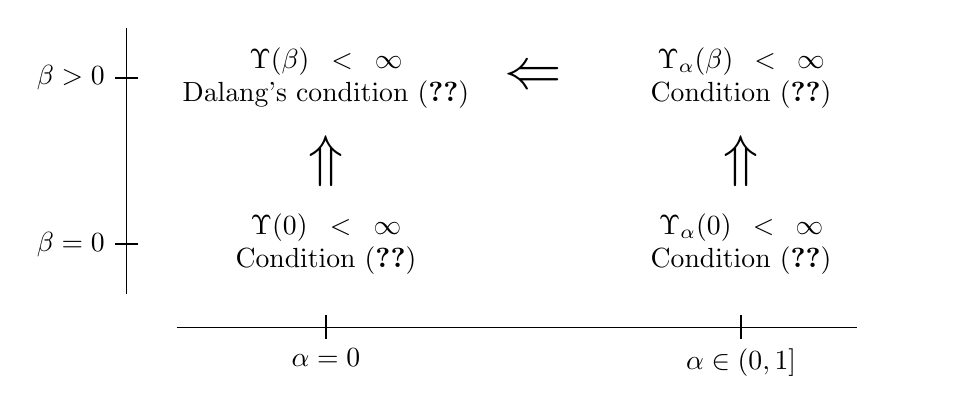
\begin{tikzpicture}[scale=1, x=6em, y=6em]
		% \tikzset{>=latex}
		\def\inc{0.07}
		\def\xo{1.2}
		\def\yo{0.5}
		\def\xg{3.7}
		\def\yg{1.5}
		\draw[] (\xo-0.9,0) -- (\xg+0.7,0);  % node[right] {$\alpha$};
		\draw[] (0,\yo-0.3) -- (0,\yg+0.3); % node[above] {$\beta$};
		\draw[thick] (\xo,\inc) --++ (0,-2*\inc) node[below] {$\alpha=0$};
		\draw[thick] (\xg,\inc) --++ (0,-2*\inc) node[below] {$\alpha\in(0,1]$};
		\draw[thick] (\inc,\yo) --++ (-2*\inc,0) node[left] {$\beta=0$};
		\draw[thick] (\inc,\yg) --++ (-2*\inc,0) node[left] {$\beta>0$};
		\node[text width=13em, align = center] (01) at (\xo,\yg) {$\Upsilon(\beta)<\infty$\\ Dalang's condition \eqref{E:Dalang}};
		\node[text width=13em, align = center] (00) at (\xo,\yo) {$\Upsilon(0)<\infty$\\ Condition \eqref{E:Dalang-00}};
		\node[text width=13em, align = center] (10) at (\xg,\yo) {$\Upsilon_\alpha(0)<\infty$\\ Condition \eqref{E:Dalang-a0}};
		\node[text width=13em, align = center] (11) at (\xg,\yg) {$\Upsilon_\alpha(\beta)<\infty$\\ Condition \eqref{E:Dalang-ab}};
		\node[] at (\xo,0.5*\yo+0.5*\yg) {\huge$\Uparrow$};
		\node[] at (\xg,0.5*\yo+0.5*\yg) {\huge$\Uparrow$};
		\node[] at (0.5*\xo+0.5*\xg,\yg) {\huge$\Leftarrow$};
		\end{tikzpicture}
	\end{center}
	
	\caption{Relations among conditions \eqref{E:Dalang}, \eqref{E:Dalang-ab}, \eqref{E:Dalang-a0} and
		\eqref{E:Dalang-00}. Check also Lemma \ref{L:HUA} for the relation between $\Upsilon(0)<\infty$
		and $\Upsilon_\alpha(0)<\infty$.}
	
	\label{F:Dalang}
\end{figure}

Note that the two conditions in \eqref{E:U0finite} guarantee the existence of the following
non-empty open interval:
\begin{align} \label{E:Interval}
\left(2^7 L_b^2 \Upsilon(0), 1\right) \ne \emptyset.
\end{align}

Now we are ready to state our two main results of the paper.

\begin{theorem} \label{T:Lrho}
	% Let $\mu(\cdot)$ be an $\mathcal{F}_0$-measurable random variable and
	Let $u(t,x;\mu)$ be the solution to \eqref{E:SHE} starting from $\mu$. Assume that
	\begin{enumerate}[(i)]
		\item $\rho: \R^d \to \R_+$ is a nonnegative $L^1(\R^d)$ function;
		\item the initial condition $\mu$ satisfies
		\begin{equation} \label{E:G}
		\mathcal{G}_{\rho}(t;\mu)
		:= \int_{\R^d} J_0^2\left(t,x;1+|\mu|\right) \rho(x)\: \ud x< \infty
		\quad \text{for all $t>0$};
		\end{equation}
		\item the spectral measure $\widehat{f}$ and the Lipschitz constant $L_b$ satisfy the two
		conditions in \eqref{E:U0finite}.
	\end{enumerate}
	Then there exists an unique $L^2(\Omega)$-continuous solution $u(t,x)$ such that for some constant
	$C>0$, which does not depend on $t$, the following holds:
	\begin{equation} \label{E:uInLrho}
	\E\left(\Norm{u(t,\cdot;\mu)}_{\rho}^2\right)
	\le C \mathcal{G}_{\rho}(t;\mu)
	< \infty, \quad \text{for any } t > 0. 
	\end{equation}
\end{theorem}

This theorem will be proved in Section \ref{S:Lrho}.

\begin{theorem} \label{T:Main}
	Let $u(t,x)$ be the solution to \eqref{E:SHE} starting from $\mu$ and let $\rho$ be an admissible
	weight function. Assume that
	\begin{enumerate}[(i)]
		\item there exists another admissible weight $\tilde{\rho}$ such that
		\begin{align} \label{E:rhorho}
		\int_{\R^d}\dfrac{\rho(x)}{\tilde{\rho}(x)}\ud x < \infty;
		\end{align}
		\item the weight function $\tilde{\rho}$ and the initial condition satisfy the following
		condition:
		\begin{equation} \label{E:InitData}
		\limsup_{t>0}\: \mathcal{G}_{\tilde{\rho}}(t;\mu) < \infty;
		\end{equation}
		\item the spectral measure $\widehat{f}$ and the Lipschitz constant $L_b$ satisfy the two
		conditions in \eqref{E:U0finite};
		\item for some $\alpha\in \left(2^7\Upsilon(0)L_b^2,1\right)$ (see \eqref{E:Interval}), the
		spectral measure $\widehat{f}$ satisfies \eqref{E:Dalang-a0}.
	\end{enumerate}
	Then we have that
	\begin{enumerate}[(a)]
		\item for any $\tau>0$, the sequence of laws of $\{\mathcal{L}u(t,\cdot;\mu)\}_{t\ge \tau}$ is
		tight, i.e., for any $\epsilon \in (0,1)$, there exists a compact set $\mathscr{K}\subset
		L^2_{\rho}(\R^d)$ such that
		\begin{equation} \label{E:cpt}
		\mathcal{L}u(t,\cdot;\mu)(\mathcal{K})
		:=  \mathbb{P}\left( u(t,\cdot;\mu) \in \mathscr{K}\: \right) \ge 1-\epsilon,
		\qquad \text{for all $t\ge \tau>0$};
		\end{equation}
		\item there exists an invariant measure for the laws $\{\mathcal{L}u(t,\cdot;\mu)\}_{t > 0}$ in
		$L^2_\rho(\R^d)$.
	\end{enumerate}
\end{theorem}

This theorem will be proved in Section \ref{S:mainproof}.
\bigskip

The work by Tessitore and Zabczyk \cite{tessitore.zabczyk:98:invariant} has a strong influence in
the current work. We formulate and solve the problem using the random field language with some
state-of-the-art moment estimates. The improvements over \cite{tessitore.zabczyk:98:invariant} consist
of the following aspects:
\begin{enumerate}
	\item Results in \cite{tessitore.zabczyk:98:invariant} allow essentially all bounded functions as
	the initial conditions, though Theorem 3.3 ({\it ibid.}) was proved only for the constant one
	initial condition. Here we give precise conditions on the initial condition, namely,
	\eqref{E:InitData}, which allows a much wider class of initial conditions, including unbounded
	functions and measures such as the Dirac delta measure; see Examples \ref{Ex:delta} and
	\ref{Ex:Riesz}. We emphasize that the Dirac delta initial measure plays a very prominent role in
	the study of the stochastic heat equation; see, e.g., \cite{amir.corwin.ea:11:probability}.
	\item We give a more easily verifiable condition in \eqref{E:Dalang-00} on the spectral density $\hat f$ and provide examples of suitable $\hat f$ in Section \ref{SS:Bassel}. Recall that due to the difficult nature of the condition (3.4) in \cite{tessitore.zabczyk:98:invariant}, no specific spectral densities were given. We further discuss this in Section \ref{SS:TessZabz}.
\end{enumerate}

This paper is organized as follows: In Section \ref{S:Example}, we will further discuss our main results and provide some examples. In particular, in Section \ref{SS:Weight}  we make some comments on the weight function and in Section \ref{SS:Init} we show that our results could include a wider class of initial conditions. Finally, the two main Theorems \ref{T:Lrho} and \ref{T:Main} will be proved in Sections \ref{S:Lrho}
and \ref{S:mainproof}, respectively.
\bigskip

Throughout the paper, we will use $\Norm{X}_p $ to denote the $L^p(\Omega)$ norm, namely,
$\left(\mathbb{E}(|X|^p)\right)^{1/p}$. We will also use the following factorization
property of the heat kernel
\begin{equation} \label{E:gsim}
G(t,x)G(s,y)=G\left(\frac{ts}{t+s}, \frac{sx + ty}{t+s}\right)G\left(t+s, x-y\right),
\end{equation}
which can be easily verified. Lastly, we remind the reader of the following spherical coordinate integration formula
\[
\int_{\R^d} f(|x|) \ud x = \sigma(\mathbb{S}^{d-1}) \int_0^\infty f(r) r^{d-1} \ud r,
\]
which we will use often and where $\sigma(\mathbb{S}^{d-1})  = 2(\pi)^{d/2} / \Gamma(d/2)$.
The convention of Fourier transform is given in Remark \ref{R:Fourier}
below.

% We reserve $C_d$ for the constant coming from the change of variable
% to the spherical coordinates:
% \begin{align*}
%   C_d := \frac{2\pi^{d/2}}{\Gamma(d/2)}.
% \end{align*}



\section{Discussions and Examples} \label{S:Example}
\subsection{Weight functions} \label{SS:Weight}
Here are several examples of admissible weights (see Example in Section 2 of
\cite{tessitore.zabczyk:98:invariant})
\begin{equation} \label{E:admRho}
\begin{aligned}
\rho(x) & = \exp(-a|x|), \quad               &  & a>0 \quad \text{and} \\
\rho(x) & = \left(1+|x|^a\right)^{-1}, \quad &  & a>d.
\end{aligned}
\end{equation}

\begin{remark} \label{R:admRho}
	The smaller the weight function $\rho(\cdot)$ (not necessarily admissible) is, the larger the
	space $L_\rho^2(\R^d)$ is. For example, one may choose $\rho$ to be either a nonnegative function
	with compact support or the heat kernel itself $G(1,\cdot)$. In both cases, $\rho$ is smaller than
	those in \eqref{E:admRho} (up to a constant). However, one can easily check that the admissible
	condition \eqref{E:aw} excludes these two cases. Lastly, we should mention that numerical results will lead one to believe that the following functions are not admissible:
	\begin{equation*}
	\rho(x) = \exp\left(-a |x|^b\right), \quad x\in\R^d,
	\quad \text{with $a>0$ and $b\in (1,2)$ fixed,}
	\end{equation*}
	but a proof of this has not yet been given.
\end{remark}

The admissible condition \ref{E:aw} is needed in this paper due to the following result:

\begin{proposition}[Proposition 2.1 of \cite{tessitore.zabczyk:98:invariant}] \label{P:weight}
	For any admissible weight $\rho$, the operators on $L^2_\rho(\R^d)$ defined by $\varphi \mapsto
	\big(G(t,\cdot)*\varphi(\cdot)\big)(x)$ can be extended to a $C_0-semigroup$ on $L^2_\rho$.
	Moreover, if $\tilde{\rho}$ is another admissible weight such that
	\begin{align*}
	\int_{\R^d}\dfrac{\rho(x)}{\tilde{\rho}(x)}\ud x < \infty,
	\end{align*}
	then for any $t>0$, the operators defined above are compact from $L^2_{\tilde{\rho}}(\R^d)$ to
	$L^2_\rho(\R^d)$.
\end{proposition}
\subsection{Various initial conditions} \label{SS:Init}

\begin{example}[$L^\infty(\R^d)$ initial condition] \label{Ex:BddInit}
	We emphasize that if the initial condition $\mu$ is deterministic and is such that $\mu(\ud x) =
	\varphi(x)\ud x$ with $\varphi\in L^\infty(\R^d)$, then all conditions related to
	$\mathcal{G}_\rho(\cdot)$ in both Theorems \ref{T:Lrho} and \ref{T:Main} are trivially satisfied.
	To be more precise, both conditions \eqref{E:G} and \eqref{E:InitData} hold because
	\begin{align*}
	\mathcal{G}_\rho(t;\varphi) \le \Norm{\varphi}_{L^\infty(\R^d)}^2 \Norm{\rho}_{L^1(\R^d)}< \infty
	\quad \text{uniformly for all $t\ge 0$.}
	\end{align*}
\end{example}

\begin{example}[Delta initial condition] \label{Ex:delta}
	In this example, we study the case when the initial condition $\mu$ is the Dirac delta measure at
	zero, namely, $\delta_0$. Let $\rho$ be a nonnegative $L^1(\R^d)$ function. Since
	\begin{align*}
	\mathcal{G}_\rho(t;\delta_0)
	= \int_{\R^d} G(t,x)^2 \rho(x) \ud x
	\le G(t,0)^2 \Norm{\rho}_{L^1(\R^d)},
	\quad \text{for all $t>0$,}
	\end{align*}
	we see that both conditions \eqref{E:G} and \eqref{E:InitData} are satisfied. In particular,
	$\limsup_{t>0} \mathcal{G}_\rho(t;\delta_0)=0$.
\end{example}


\begin{example}[More initial conditions not in $L_\rho^2(\R^d)$] \label{Ex:Riesz}
	In this example, we study the case when $\mu(\ud x) = |x|^{-\alpha}\ud x$ for some $\alpha\in
	(0,d)$. It is clear that when $\alpha\in (d/2,d)$, $\mu\not\in L_\rho^2(\R^d)$. However, in this
	case, we have
	\begin{align*}
	J_0(t,x) = \left(G(t,\cdot)* |\cdot|^{-\alpha}\right)(x)
	\le \left(G(t,\cdot)* |\cdot|^{-\alpha}\right)(0).
	\end{align*}
	On the other hand,
	Hence,
	\begin{align*}
	\left(G(t,\cdot)* |\cdot|^{-\alpha}\right)(0)
	= \frac{2\pi^{d/2}}{\Gamma(d/2)}\times (2\pi t)^{-d/2} \int_0^\infty e^{-\frac{r^2}{2t}} r^{-\alpha + d-1} \ud r = C_* t^{-\alpha/2},
	\end{align*}
	with $C_*=2^{-\alpha/2}\Gamma\left((d-\alpha)/2\right)/\Gamma(d/2)$, which implies that
	\begin{align*}
	\mathcal{G}_\rho\left(t;|\cdot|^{-\alpha}\right)
	\le \int_{\R^d} J_0^2(t,0) \rho(x) \ud x
	= C_*^2 t^{-\alpha} \Norm{\rho}_{L^1(\R^d)},
	\quad \text{for all $t>0$.}
	\end{align*}
	Therefore, we see that both conditions \eqref{E:G} and \eqref{E:InitData} are satisfied.
\end{example}

The following proposition shows that for initial conditions with unbounded tails, condition
\eqref{E:G} may hold while condition \eqref{E:InitData} may fail.

\begin{proposition} \label{P:growtail}
	Suppose that $\rho=\exp(-|x|)$, which is an admissible weight function. Let the initial condition
	$\mu$ be given as
	\begin{align*}
	\mu(\ud x) = |x|^\alpha \ud x \quad \text{with $\alpha>0$}.
	\end{align*}
	Then for some constants $C, C'>0$ that depend on $d$ and $\alpha$, it holds that
	\begin{align} \label{E:growtail}
	C' (1+t^\alpha) \le \mathcal{G}_\rho(t;\mu) \le C (1+t^\alpha), \qquad \text{for all $t>0$}.
	\end{align}
	In particular, this implies that condition \eqref{E:G} is satisfied, but condition
	\eqref{E:InitData} fails.
\end{proposition}
\begin{proof}
	Notice that by scaling arguments,
	\begin{align*}
	\mathcal{G}_\rho(t;\mu)
	& = \int_{\R^d} \left(\int_{\R^d}G(t,x-y) |y|^\alpha \ud y\right)^2 e^{-|x|} \ud x                                        \\
	& = \int_{\R^d}t^\alpha \left(\int_{\R^d}G\left(1,\frac{x}{\sqrt{t}}-z\right) |z|^\alpha \ud z\right)^2 e^{-|x|} \ud x    \\
	& = \int_{\R^d}t^{\alpha+d/2} \left(\int_{\R^d}G\left(1,\xi-z\right) |z|^\alpha \ud z\right)^2 e^{-\sqrt{t}|\xi|} \ud \xi.
	\end{align*}
	In the following, let $C_d$, $C_\alpha$, $C_\alpha'$, $C_{\alpha, d}$ and $C'_{\alpha, d}$ be generic constants that may depend on
	$\alpha $ and $d$ and may change their value at each appearance. \bigskip
	
	\noindent{\it Upper bound:~} Because
	\begin{align*}
	% \int_{\R^d}G\left(1,\xi-z\right) |z|^\alpha \ud z
	\int_{\R^d}G\left(1,z\right) |\xi-z|^\alpha \ud z
	\le C_\alpha \int_{\R^d}G\left(1,z\right) \left(|\xi|^\alpha + |z|^\alpha\right) \ud z
	\le C_\alpha' \left( 1+|\xi|^\alpha\right),
	\end{align*}
	we see that
	\begin{align*}
	\mathcal{G}_\rho(t;\mu)
	& \le C_\alpha \int_{\R^d}t^{\alpha+d/2} \left(1+|\xi|^{2\alpha}\right) e^{-\sqrt{t}|\xi|} \ud \xi \\
	& = C_{\alpha, d}\int_{0}^{\infty}t^{\alpha+d/2} \left(1+r^{2\alpha}\right) e^{-\sqrt{t}r}r^{d-1} \ud r        \\
	& = C_{\alpha, d} \left(t^\alpha \Gamma(d) + \Gamma(d+2\alpha)\right)                                   \\
	& = C'_{\alpha, d} (1+ t^\alpha)<\infty.
	\end{align*}
	Hence, this proves the upper bound in \eqref{E:growtail}. \bigskip
	
	\noindent{\it Lower bound:~} Now we prove the lower bound in \eqref{E:growtail}. Indeed,
	\begin{align*}
	\int_{\R^d}G\left(1,z\right) |\xi-z|^\alpha \ud z
	& \ge \int_{\R^d}G\left(1,z\right) \big| |\xi| - |z| \big|^\alpha \ud z \\
	&  \ge {C_d} \int_0^\infty \big| |\xi| - x \big|^\alpha e^{-\frac{x^2}{2}}x^{d-1}\ud x \\
	&  \ge C_d \int_1^2 \big| |\xi| - x \big|^\alpha \ud x \\
	&  = \frac{C_d}{1+\alpha} \psi\left(|\xi|\right),
	\end{align*}
	where, by considering three cases, we have
	\begin{align*}
	\psi(r)
	& =
	\begin{cases}
	(2-r)^{\alpha+1} - (1-r)^{\alpha+1} & \text{if $0<r<1$},        \\
	(2-r)^{\alpha+1} + (r-1)^{\alpha+1} & \text{if $1\le r \le 2$}, \\
	(r-1)^{\alpha+1} - (r-2)^{\alpha+1} & \text{if $r > 2$},
	\end{cases} \\
	& = \text{sgn}(2-r)|r-2|^{\alpha+1} + \text{sgn}(r-1)|r-1|^{\alpha+1}.
	\end{align*}
	We claim that
	\begin{align} \label{E:psi}
	\inf_{r\ge 0} \frac{\psi(r)}{\sqrt{1+r^{2\alpha}}}>0.
	\end{align}
	With \eqref{E:psi}, we have that
	\begin{align*}
	\int_{\R^d}G\left(1,z\right) |\xi-z|^\alpha \ud z \ge C_{\alpha, d} \sqrt{1+|\xi|^{2\alpha}}.
	\end{align*}
	Then, by the same arguments as above for the upper bound, we obtain the lower bound in \eqref{E:growtail}. It remains to prove
	\eqref{E:psi}, which will be proved in three cases.
	
	When $r>2$, we see that
	\begin{align*}
	\frac{\psi(r)}{\sqrt{1+r^{2\alpha}}}
	& \ge C_\alpha \frac{(r-1)^{\alpha+1}-(r-2)^{\alpha+1}}{(1+r)^\alpha}       \\
	& \ge C_\alpha \frac{(r-1)^{\alpha}(r-1)-(r-1)^{\alpha}(r-2)}{(1+r)^\alpha} \\
	& = C_\alpha \left(\frac{r-1}{1+r}\right)^\alpha
	= C_\alpha \left(1-\frac{2}{1+r}\right)^\alpha \ge C_\alpha \left(1-\frac{2}{3}\right)^\alpha.
	\end{align*}
	Note that in the first inequality above, we have considered two
	cases: $2\alpha \ge 1$ and $2 \alpha < 1$. When $2\alpha < 1$, we have used the concavity of
	$x^{2\alpha}$, namely, $ (1 + r^{2\alpha})^{2\alpha} / 2 \le ((1+r)/2)^{2\alpha}$; when $2\alpha
	\ge 1$, we have used the super-additiity of $x^{2\alpha}$: namely, that for $a,b>0$ that $
	(a+b)^{2\alpha}\ge a^{2\alpha} + b^{2\alpha}$. This shows that $\inf_{r>2}
	\frac{\psi(r)}{\sqrt{1+r^{2\alpha}}} >0$.
	
	When $r\in(1,2]$, elementary calculations show that the minimum of $\psi(r)$ is achieved at
	$r=3/2$. Hence,
	\begin{align*}
	\inf_{r\in(1,2]} \frac{\psi(r)}{\sqrt{1+r^{2\alpha}}} \ge \frac{\psi(3/2) }{\sqrt{1+4^\alpha}}>0.
	\end{align*}
	
	Similarly, when $r\in (0,1]$, by differentiation, one finds that the function $\psi(r)$ is nonincreasing.
	Hence, the minimum is achieved at $r=1$:
	\begin{align*}
	\inf_{r\in(0,1]} \frac{\psi(r)}{\sqrt{1+r^{2\alpha}}} \ge \frac{\psi(1) }{\sqrt{2}}>0.
	\end{align*}
	
	Combing the above three cases proves \eqref{E:psi}. This completes the proof of Proposition
	\ref{P:growtail}.
\end{proof}

\subsection{Bessel kernel and Mat\'ern class of correlation functions} \label{SS:Bassel}

\begin{example}[Bessel kernel as a correlation function] \label{Ex:Gamma+f}
	Let $f_s$ denote the Bessel kernel with a strictly positive parameter $s>0$. It is known that
	(see, e.g., Section 1.2.2 of \cite{grafakos:14:modern})
	\begin{enumerate}
		\item $f_s(x)>0$ for all $x\in\R^d$ and $ \Norm{f_s}_{L^1(\R^d)}=1$;
		\item there exists a constant $C(s,d)>0$ such that
		\begin{align*}
		f_s(x) \le C(s,d) \exp(-|x|/2) \quad \text{for} \quad |x| \ge 2;
		\end{align*}
		\item there exists a constant $c(s,d)>0$ such that
		\begin{gather*}
		\frac{1}{c(s,d)} \le \frac{f_s(x)}{H_s(x)} \le c(s,d) \quad \text{for} \quad |x| \le 2, \quad \text{with} \\
		H_s(x) =
		\begin{cases}
		|x|^{s-d} + 1 + O(|x|^{s-d+2})                  & \text{for $0<s<d$,} \\
		\log\left(\frac{2}{|x|}\right) + 1 + O(|x|^{2}) & \text{for $s=d$,}   \\
		1 + O(|x|^{s-d})                               & \text{for $s>d$;}
		\end{cases}
		\end{gather*}
		\item the Fourier transform of $f_s$ is strictly positive:
		\begin{equation} \label{E:FB}
		\mathcal{F}f_s(\xi) = \frac{1}{(1+|\xi|^2)^{s/2}}.
		\end{equation}
	\end{enumerate}
	Note that one can use \eqref{E:FB} as the definition of the Bessel kernel. Properties 1 and 4 ensure
	that $f_s$ is a nonnegative and nonnegative-definite tempered measure for all $s>0$. From Property
	4, we see that
	\begin{align*}
	\Upsilon(0)<\infty \quad \Longleftrightarrow \quad  s>d-2.
	\end{align*}
	In the following, we will assume that $s>d-2$ and $d\ge 3$.
\end{example}

\begin{example}[Mat\'ern class of correlation functions]
	The {\it Mat\'ern class of correlation functions} has been widely used in spatial statistics; one
	may check the recent work \cite{loh.sun.ea:21:on} for references. Following Section 2.10 of
	\cite{stein:99:interpolation}, this class of correlation functions is given by
	\begin{align} \label{E:Matern}
	K(x) = \phi \cdot (\alpha |x|)^\nu \mathcal{K}_\nu\left(\alpha |x|\right), \quad  \text{for
		$x\in\R^d$ with }\phi>0, \alpha>0, \nu >0 ,
	\end{align}
	where $\mathcal{K}_\nu(\cdot)$ is the modified Bessel function of second type, and $\alpha$ and $\nu$
	refer to the {\it scaling and smoothness parameters} respectively. From the inversion formula
	(see p. 46 {\it ibid.}), one sees that
	\begin{align*}
	\mathcal{F}K(\xi) = (2\pi)^{d} \mathcal{F}^{-1} K(\xi) = (2\pi)^d f(|\xi|)
	\quad \text{with} \quad
	f(\xi) = \frac{2^{\nu-1} \phi \Gamma\left(\nu +d/2\right)\alpha^{2\nu}}{\pi^{d/2}\left(\alpha^2+|\xi|^2\right)^{\nu+d/2}}, \quad  \xi\in\R^d.
	\end{align*}
	Comparing the above expression with \eqref{E:FB}, we see that the class of Bessel kernels $f_s$,
	with $s>d-2$ and $d\ge 3$, includes the Mat\'ern class \eqref{E:Matern} as a special case under
	the following choice of parameters:
	\begin{align*}
	\alpha = 1,\quad \nu=(s-d)/2,\quad  \text{and} \quad \phi= 2^{(2-d-s)/2} \pi^{-d/2} \Gamma(s /2)^{-1}.
	\end{align*}
	Note that the requirement of the smoothness parameter $\nu>0$ for the Mat\'ern class corresponds
	to the case of the Bessel kernel with $s>d$.
\end{example}

For $\alpha \in (0, 1/2)$, we introduce the following quantity which will now be needed throughout this article:
\begin{equation} \label{E:H}
\mathcal{H}_{\alpha}(t) := \int_0^t \ud r \: r^{-2\alpha} \int_{\R^d} \hat{f}(\ud \xi) \: \exp(-r|\xi|^2)
\end{equation}

\begin{proposition} \label{P:Bessel}
	For the Bessel kernel $f_s(\cdot)$ with $s>0$ defined in Example \ref{Ex:Gamma+f}, it holds that
	\begin{gather} \label{E:UpsionB}
	\Upsilon_{\alpha}(0) = \frac{\Gamma\left(\frac{d}{2} -1 + \alpha\right) \Gamma\left( \frac{s-d}{2} + 1 - \alpha \right)}{2^d \pi^{d/2} \: \Gamma(d/2)\:\Gamma\left(s/2\right)}
	\qquad \text{for all $s>d-2(1-\alpha) > 0$ and $d>2$,}
	\end{gather}
	and in particular when $\alpha = 0$, \eqref{E:UpsionB} simplifies to the following:
	\begin{equation} \label{E:Upsilon_0}
	\Upsilon(0) = \frac{ \Gamma\left(\frac{2+s-d}{2}\right)}{2^{d-1} \pi^{d/2} (d-2)\Gamma(s/2)}.
	\end{equation}
	In addition,
	\begin{gather}\label{E:HaB} 
	\mathcal{H}_\alpha(t) <\infty \quad \forall t>0 \quad \Longleftrightarrow \quad
	0<\alpha<\frac{1}{2} - \frac{(d-s)_+}{4}\quad \text{and} \quad s>d-2>0,
	\end{gather}
	where $a_+ := \max(a,0)$.
	Moreover, for $\alpha\in(0,1/2)$, we have the following asymptotic behavior of
	$\mathcal{H}_\alpha(t)$ at $t\to 0$: % \renewcommand{\arraystretch}{2}
	\begin{align} \label{E:HaBS}
	\mathcal{H}_\alpha(t) = \left\{
	\begin{array}{lcl}
	\begin{aligned}
	\dfrac{\pi^{d/2} \Gamma\left((d-s)/2\right)}{\left((s-d)/2+1-2\alpha\right)\Gamma(d/2)}  t^{(s-d)/2+1-2\alpha}                  \\[1em]
	\quad - \dfrac{\pi^{d/2}\Gamma\left((s-d)/2\right)}{(1-2\alpha)\Gamma(s/2)}              t^{1-2\alpha}                          \\[1em]
	+                                                                                        O\left(t^{(s-d)/2+2(1-\alpha)}\right), \\[1.2em]
	\end{aligned}
	&
	\begin{gathered}
	d-2<s<d    \\
	\text{and} \\
	\alpha < \frac{1}{2} -\frac{1}{4}(d-s)
	\end{gathered} & \text{\em(\ref{E:HaBS}-a)} \\
	\begin{aligned}
	\frac{\pi ^{d/2}}{(1-2 \alpha) \Gamma \left(d/2\right)}t^{1-2\alpha}\log\left(\frac{1}{t}\right)                                    \\[1em]
	+\frac{\pi ^{d/2} \left(1- (1-2 \alpha) \left[\psi(d/2)+2\gamma\right]\right)}{(1-2 \alpha)^2 \Gamma \left(d/2\right)}t^{1-2 \alpha} \\[1em]
	+O\left(t^2\log(t)\right),                                                                                                           \\[1.2em]
	\end{aligned}                                                                                                           & s=d     & \text{\em(\ref{E:HaBS}-b)} \\ [1em]
	\dfrac{\pi^{d/2}\Gamma\left((s-d)/2\right)}{(1-2\alpha)\Gamma(s/2)}t^{1-2\alpha} + O\left(t^{(s-d)/2+1-2\alpha}\right), & d<s<d+2 & \text{\em(\ref{E:HaBS}-c)} \\ [1.5em]
	\dfrac{\pi^{d/2}}{(1-2\alpha)\Gamma\left(d/2+1\right)}t^{1-2\alpha}  + O\left(t^{2(1-\alpha)}\log(t)\right),            & s=d+2   & \text{\em(\ref{E:HaBS}-d)} \\ [1.5em]
	\dfrac{\pi^{d/2}}{(1-2\alpha)\Gamma\left(d/2+1\right)}t^{1-2\alpha}  + O\left(t^{2(1-\alpha)}\right),                   & s>d+2   & \text{\em(\ref{E:HaBS}-e)} \\ [1.5em]
	\end{array}
	\right.
	\end{align}
	where $\psi(x)=\frac{\ud}{\ud x}\log\Gamma(x)$ refers to the {\em digamma function} and
	$\gamma\approx 0.57721$ to {\em Euler's constant}; see, e.g., 5.2.2 and 5.2.3 on p. 136 of
	\cite{askey.roy:10:gamma}.
\end{proposition}

\begin{proof}
	By the spherical coordinate integration formula and \eqref{E:FB}, for all $\alpha\in[0,1)$,
	\begin{align*}
	\Upsilon_\alpha(0) = \left(2\pi\right)^{-d} \int_{\R^d} \frac{\ud\xi}{|\xi|^{2(1-\alpha)}\left(1+|\xi|^2\right)^{s/2}}
	= \left(2\pi\right)^{-d} C_d \int_0^\infty \frac{r^{d-1}}{r^{2(1-\alpha)}\left(1+r^2\right)^{s/2}} \ud r,
	\end{align*}
	where $C_d:=\frac{2\pi^{d/2}}{\Gamma\left(d/2\right)}$. Now by the change of variables $z=r^2/(1+r^2)$,
	we can evaluate the above integral explicitly by transforming it to the Beta integral:
	\begin{align*}
	\int_0^\infty \frac{r^{d-1}}{r^{2(1-\alpha)}\left(1+r^2\right)^{s/2}} \ud r
	& = \frac{1}{2} \int_0^1 z^{d/2+\alpha-2}(1-z)^{(s-d)/2-\alpha}\ud z \\
	& = \frac{\Gamma\left(d/2-1+\alpha\right)\Gamma\left((s-d)/2+1-\alpha\right)}{2\Gamma(s/2)},
	\end{align*}
	which is finite provided that $s>d-2(1-\alpha)>0$. This proves \eqref{E:UpsionB} and from this, we easily deduce \eqref{E:Upsilon_0} by letting $\alpha = 0$ in \eqref{E:UpsionB} and by applying the formula $\Gamma(z+1) = z\Gamma(z)$, which holds for $z\in \mathbb{C}$ such that $\Re(z)>0$. 
	
	It remains to prove \eqref{E:HaBS}, which then implies \eqref{E:HaB}. From \eqref{E:H} and by the
	spherical coordinate integration formula, for all $t>0$,
	\begin{align*}
	\mathcal{H}_{\alpha}(t)
	& = \int_0^t \ud r \; r^{-2\alpha} \int_{\R^d} \ud \xi \; \frac{\exp(-r|\xi|^2)}{ (1+|\xi|^2)^{s/2}}     \\
	& = C_d \int_0^t \ud r \; r^{-2\alpha} \int_0^\infty \ud z \; \frac{\exp(-r z^2)}{(1+z^2)^{s/2}} z^{d-1} \\
	& = \frac{C_d}{2} \int_0^t \ud r \; r^{-2\alpha} \int_0^\infty \ud u \; \exp(-r u)(1+u)^{-s/2} u^{d/2-1} \\
	& =: \frac{C_d \Gamma\left(d/2\right)}{2} \int_0^t \ud r \; r^{-2\alpha} I(r) = \pi^{d/2}\int_0^t \ud r \; r^{-2\alpha} I(r).
	% & = C_d \int_0^t \ud r \; r^{-2\alpha+ (s-d) /2} \int_0^\infty \ud z \; \frac{\exp(-z^2)}{(r+z^2)^{s/2}} z^{d-1}.
	\end{align*}
	By \cite[13.4.4 on p.326]{olde-daalhuis:10:confluent}, $I(r)$ is equal to the {\it confluent
		hypergeometric function}:
	\begin{align*}
	I(r) =U\left(\frac{d}{2},\frac{2+d-s}{2},r\right).
	\end{align*}
	By 18.2.18 -- 13.2.22 on p. 323 {\it ibid.}, we see that \renewcommand{\arraystretch}{2}
	\begin{align*}
	I(r) = \left\{
	\begin{array}{lcl}
	\dfrac{\Gamma\left((d-s)/2\right)}{\Gamma(d/2)}r^{(s-d)/2}+\dfrac{\Gamma\left((s-d)/2\right)}{\Gamma(s/2)} + O\left(r^{(s-d)/2+1}\right) & d-2<s<d & \text{\small 18.2.18}, \\
	-\dfrac{1}{\Gamma(d/2)}\left(\log(r) + \psi(d/2) + 2\gamma \right) +O\left(r\log(r)\right)                                               & s=d     & \text{\small 18.2.19}, \\
	\dfrac{\Gamma\left((s-d)/2\right)}{\Gamma(s/2)} + O\left(r^{(s-d)/2}\right)                                                              & d<s<d+2 & \text{\small 18.2.20}, \\
	\dfrac{1}{\Gamma\left(d/2+1\right)} + O\left(r\log(r)\right)                                                                             & s=d+2   & \text{\small 18.2.21}, \\
	\dfrac{\Gamma\left((s-d)/2\right)}{\Gamma(s/2)} + O\left(r\right)                                                                        & s>d+2   & \text{\small 18.2.22}. \\
	\end{array}
	\right.
	\end{align*}
	Then integrating the right-hand side of the above expressions against $\pi^{d/2}r^{-2\alpha}\ud r$
	over $[0,t]$ gives the five cases in \eqref{E:HaBS}. This completes the proof of Proposition
	\ref{P:Bessel}.
\end{proof}

\subsection{A discussion on Tessitore and Zabczyk's condition} \label{SS:TessZabz}

In the setting of equation \eqref{E:SHE}, Tessitore and Zabczyk
\cite{tessitore.zabczyk:98:invariant} prove the existence of an invariant measure for \eqref{E:SHE} in
$L^2_{\rho}(\R^d)$ under the assumption that there exists a $\varphi \in L^2_{\rho}(\R^d) \cap
L^2_{\widetilde\rho}(\R^d)$ where $\rho (\widetilde\rho)^{-1} \in L^1(\R^d)$ and the solution
starting from $\varphi$ is bounded in probability in $L^2_{\widetilde \rho}(\R^d)$ and also that the
spectral density $\hat{f}$ satisfies
\begin{equation} \label{E:CorTZ}
\widehat{f} \in L^p(\R^d) \quad \text{where } \frac{d-2}{d} < \frac{1}{p};
\end{equation}
see Hypothesis 2.1 ({\it ibid.}). However as was illustrated in \cite[Theorem
3.3]{tessitore.zabczyk:98:invariant}, in order to apply this theorem to a specific initial condition in $L^2_{\rho}$ (or to have moments uniformly
bounded in time), the following additional
assumptions were imposed:
\begin{equation} \label{E:TZspec}
d\ge 3 \quad \text{and} \quad
L_b^{-2}> \frac{\Gamma(d/2 -1)2^{d/2-2}}{(2\pi)^{2d}} \int_{\R^d} \left(\left|  \mathcal{F}\left(\sqrt{ \widehat{f}\: }\right) \right| * \left| \mathcal{F}\left(\sqrt{ \widehat{f}\: }\right)\right|\right) (\zeta) |\zeta|^{2-d} \ud \zeta ,
\end{equation}
where $\Gamma$ refers to the Gamma function; see Remark \ref{R:Fourier}. With these assumptions,
they were able to prove that \eqref{E:SHE} starting from the constant $1$ satisfies \eqref{E:BddMnt}
and thus is bounded in probability, verifying the existence of an invariant measure. Moreover, the
measure takes the form of \eqref{E:InvMeasForm} above with $\varphi = 1$. Lastly we mention that due to its difficult nature, \eqref{E:TZspec} was not calculated for a specific $\widehat{f}$ (see Examples \ref{Ex:Finv} and \ref{Ex:sqrt} below).

\begin{remark} \label{R:Fourier}
	The Fourier transform may be defined differently depending how to handle the $2\pi$ constant. In
	this paper (as in \cite{chen.kim:19:nonlinear,chen.huang:19:comparison}), we use the convention
	that
	\begin{align} \label{E:Fourier}
	\widehat{\phi}(\xi)      = \mathcal{F}\phi(\xi) := \int_{\R^d} e^{-i x\cdot\xi} \phi(x)\ud x \quad \text{and} \quad
	\mathcal{F}^{-1}\psi(x) := (2\pi)^{-d} \int_{\R^d} e^{i x\cdot\xi} \psi(\xi)\ud \xi.
	\end{align}
	Hence, Plancherel's theorem takes the form of
	\begin{align} \label{E:Plancherel}
	\int_{\R^d} \psi(x) \phi(x)\ud x = (2\pi)^{-d} \int_{\R^d} \widehat{\psi}(\xi) \overline{\widehat{\phi}(\xi)}\ud \xi.
	\end{align}
	Note that the authors in \cite{tessitore.zabczyk:98:invariant} did not explicitly mention their convention of the Fourier transform. However, the proof of Theorem 3.3 ({\it ibid.}) suggests that
	the following convention has been used:
	\begin{align*}
	\widehat{\phi}(\xi)      = \mathcal{F}\phi(\xi) := (2\pi)^{-d/2} \int_{\R^d} e^{-i x\cdot\xi} \phi(x)\ud x \quad \text{and} \quad
	\mathcal{F}^{-1}\psi(x) := (2\pi)^{-d/2} \int_{\R^d} e^{i x\cdot\xi} \psi(\xi)\ud \xi.
	\end{align*}
	Hence, Plancherel's theorem takes the form, $\int_{\R^d} \psi(x) \phi(x)\ud x = \int_{\R^d}
	\widehat{\psi}(\xi) \overline{\widehat{\phi}(\xi)}\ud \xi$, without the additional factor
	$(2\pi)^{-d}$. In particular, the spectral density $\gamma$ ({\it ibid.})
	corresponds to $\left(2\pi\right)^{-d/2}\widehat{f}$ in this paper. Our equation \eqref{E:TZspec}, which is condition (3.4) \cite{tessitore.zabczyk:98:invariant}, takes into account this difference therefore explaining the slightly
	different factor in front of the integral in \eqref{E:TZspec} from that in (3.4) ({\it ibid.}).
\end{remark}

Recall the definition of $\mathcal{F}^{-1}$ in \eqref{E:Fourier} above. We may rewrite the integral in the second condition of \eqref{E:TZspec} as follows:
\begin{align*}
\Gamma(d/2 -1)2^{d/2-2} \int_{\R^d} \left(\left| \mathcal{F}^{-1}\left(\sqrt{ \widehat{f}\: }\right) \right| * \left| \mathcal{F}^{-1}\left(\sqrt{ \widehat{f}\: }\right)\right|\right) (\zeta) |\zeta|^{2-d} \ud \zeta.
\end{align*}
We now consider a couple of situations and give two examples that illustrate some of the difficulties that may arise. \bigskip

{\bf\noindent Case I:~} If both $\mathcal{F}^{-1}\left[\sqrt{\widehat{f}(\cdot)}\right](\xi)$ and $\widehat{f}$ are strictly positive for all $\zeta\in\R^d$, which is not a trivial assumption (see Example \ref{Ex:Finv} below), then
there is no ambiguity when taking the square root and one can remove the absolute value to see
that
\begin{align*}
\Gamma(d/2 -1)2^{d/2-2} & \int_{\R^d} \left(\mathcal{F}^{-1}\left(\sqrt{ \widehat{f}\: }\right) * \mathcal{F}^{-1}\left(\sqrt{ \widehat{f}\: }\right)\right) (\zeta) |\zeta|^{2-d} \ud \zeta \\
& = \frac{1}{(2\pi)^{3d/2}} \int_{\R^d} \widehat{f}(\zeta)  |\zeta|^{-2} \ud \zeta
= \left(2\pi\right)^{d/2}\Upsilon(0),
\end{align*}
where we have applied Plancherel's theorem (see \eqref{E:Plancherel}) and the Fourier transform
for Riesz kernel (in the generalized sense):
\begin{align*}
\mathcal{F}(|\cdot|^{-\alpha})(\xi) = \pi^{-d /2} 2^{-\alpha} \frac{\Gamma\left((d-\alpha)/2\right)}{\Gamma(\alpha /2)} |\xi|^{-(d-\alpha)},
\quad \text{for $\alpha\in(0,d)$ and $\xi\in\R^d$}.
\end{align*}
Hence, the second condition in \eqref{E:TZspec} can be equivalently written as $L_b^{-2}>
(2\pi)^{d/2}\Upsilon(0)$. Comparing this with \eqref{E:Lipb}, namely, $L_b^{-2}> 128 \Upsilon(0)$,
our condition is sharper when $d> \frac{14\log(2)}{\log(2\pi)} \approx 5.28$. 

\begin{example} \label{Ex:Finv}
	One should note that the assumption that $\mathcal{F}^{-1}\left(\sqrt{\widehat{f}}\right)(\zeta)$ is nonnegative is quite strong and requires $\sqrt{\widehat{f}}$ to be non-negative definite, which may not be true even if $f$ is non-negative and non-negative definite. Indeed, suppose that $f$ was such that $\widehat{f}(\xi) = 2^{-2}\max\{2-|\xi|,0\}$. Then $f$ is non-negative and non-negative definite, which is shown in Example \ref{Ex:sqrt} below. We will now show that in this case, $\mathcal{F}^{-1}\left(\sqrt{\widehat{f}}\right)(\zeta)$ takes on both positive and negative values. Since $\sqrt{\widehat{f}(\xi)} = 2^{-1}\sqrt{\max\{2-|\xi|,0\}}$ is even, the inverse Fourier transform takes the following form:
	\[
	\mathcal{F}^{-1}\left(\sqrt{\widehat{f}}\right)(\zeta) = 2 \int_0^2 2^{-1}\sqrt{2-x} \cos(x\: \zeta) \ud x.
	\]
	For simplicity, we will only consider the case $\zeta>0$ and real. Therefore 
	\begin{align*}
	\mathcal{F}^{-1}\left(\sqrt{\widehat{f}}\right)(\zeta) &= \int_0^2 \sqrt{x} \cos((2-x)\: \zeta) \ud x \\ 
	& = 2 \int_0^{\sqrt{2}} x^2 \cos(2\zeta- \zeta x^2) \ud x \\
	&= 2\cos(2\zeta) \int_0^{\sqrt{2}} x^2 \cos(\zeta x^2) \ud x  +2 \sin(2\zeta) \int_0^{\sqrt{2}} x^2 \sin(\zeta x^2) \ud x.
	\end{align*}
	Where in the first equality we used the change of variables, $x' = 2 - x$ and in the second equality we used the the change of variables $x' = \sqrt{x}$. We now do an integration by parts to see that 
	\begin{align*}
	\mathcal{F}^{-1}\left(\sqrt{\widehat{f}}\right)(\zeta) &= - \cos(2y) \int_0 ^{\sqrt{2}} \frac{\sin(x^2 \zeta)}{\zeta} \ud x + \sin(2\zeta) \int_0 ^{\sqrt{2}} \frac{\cos(x^2 \zeta)}{\zeta} \ud x,
	\end{align*}
	and lastly we apply the change of variables $x' = x\sqrt{2\zeta/\pi}$ too see 
	\[
	\mathcal{F}^{-1}\left(\sqrt{\widehat{f}}\right)(\zeta) = \frac{ \sqrt{\frac{\pi}{2}}\left(-\cos(2\zeta)\mathcal{S}\left(\frac{2\sqrt{\zeta}}{\sqrt{\pi}}\right) + \sin(2\zeta) \mathcal{C}\left( \frac{2 \sqrt{\zeta}}{\sqrt{\pi}} \right) \right)}{ \zeta^{3/2} },
	\]
	
	\begin{figure}
		\centering
		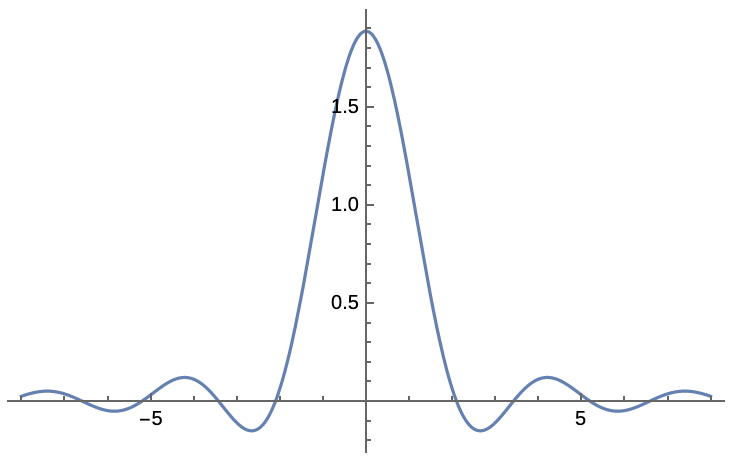
\includegraphics[scale=.9]{figs/fresnel.png}
		\caption{A plot of  $\mathcal{F}^{-1}\left(\sqrt{\widehat{f}}\right)(\zeta)$ for $\widehat{f}(\xi) = 2^{-2}\max\{2-|\xi|,0\}$ with $-8 \le \zeta \le 8$.}
	\end{figure}
	
	where $\mathcal{S}$ and $\mathcal{C}$ are the Fresnel integrals (see \cite[7.2 (iii)]{olver.lozier.ea:10:nist}):
	\[
	\mathcal{S}(z) = \int_0^{z} \sin\left(\frac{\pi t^2}{2}\right) \ud t \quad \text{and} \quad \mathcal{C}(z) = \int_0^z \cos\left(\frac{\pi t^2}{2}\right) \ud t. 
	\]
	Thus even if $f$ is both non-negative and non-negative definite, we may still have problems with removing the absolute value sign. 
\end{example}
\bigskip

{\bf\noindent Case II:~} Suppose $\widehat{f}(\cdot)$ is not strictly positive, but only nonnegative, namely, $\widehat{f}(\xi)=0$ for some $\xi\in\R^d$. Then removing the absolute value in
\eqref{E:TZspec} becomes tricky, which will be illustrated in the following example.

\begin{example} \label{Ex:sqrt}
	Let $d=1$ and $g(x)=\frac{1}{2}1_{[-1,1]}(x)$. It is clear that $ \widehat{g}(\xi) =
	\xi^{-1}\sin(\xi)$. Now set $f(x) = \left(g*g\right)(x) = 2^{-2}\max(2-|x|,0)$. It is clear that $f$
	is nonnegative. It is also nonnegative-definite because $\widehat{f}(\xi)= \widehat{g}(\xi)^2=
	\xi^{-2}\sin^2(\xi)\ge 0$. But in this case, $\widehat{f}(\cdot)$ is only nonnegative (not
	strictly positive) with infinitely many zeros. Hence, when taking the square root of
	$\widehat{f}(\xi)$ as in \eqref{E:TZspec}, one needs to wisely choose the correct positive and
	negative branches:
	\begin{enumerate}
		\item Clearly, the signed version $\sqrt{\widehat{f}(\xi)}=\xi^{-1}\sin(\xi)$ is preferable
		since its inverse Fourier transform can be easily computed, which is equal to $g(x)$.
		Moreover, because this inverse Fourier transform $g(x)$ is clearly nonnegative, the absolute
		value signs in \eqref{E:TZspec} do not pose any additional restrictions.
		\item However, if one chooses the positive branches, namely,
		$\sqrt{\widehat{f}(\xi)}=\left|\xi^{-1}\sin(\xi)\right|$, then it is not clear how to compute its
		Fourier transform. In general, some bad choices of the positive/negative branches may make the
		conditions in \eqref{E:TZspec} fail. For example, such choice may turn
		$\sqrt{\widehat{f}(\xi)}$ into a distribution, and then taking the absolute value of a
		distribution (unless it is a measure) may be problematic. Another issue that may arise is when $\sqrt{\widehat{f}(\xi)}$ is a well-defined function, taking on both positive and negative values and after taking the absolute value, the integral in \eqref{E:TZspec} may blow up. 
	\end{enumerate}
\end{example}

\section{Moment Estimates -- Proof of Theorem \ref{T:Lrho}} \label{S:Lrho}
We first state some known results and prove a moment bound in Corollary \ref{C:Mom}.

\begin{theorem}[Theorem 1.2 \cite{chen.huang:19:comparison}] \label{T:Solve}
	Suppose that
	\begin{enumerate}[(i)]
		\item the initial deterministic measure $\mu$ satisfies
		the following integrability condition:
		\begin{equation} \label{A:icon}
		\int_{\R^d}\exp\left(-a|x|^2\right) |\mu|(\ud x) < \infty \quad \text{for all $a>0$},
		\end{equation}
		\item the spectral measure $\widehat{f}$ satisfies {\it Dalang's condition} \eqref{E:Dalang},
	\end{enumerate}
	Then \eqref{E:SHE} has a unique random field solution starting from $\mu$. Moreover, the solution
	is $L^2(\Omega)$ continuous and is adapted to the filtration $\{\mathcal{F}_t\}_{t\ge 0}$.
\end{theorem}

\begin{theorem}[Theorem 1.7 \cite{chen.huang:19:comparison}] \label{T:ExUn}
	Under the assumptions of Theorem \ref{T:Solve}, for any $t>0$, $x \in \R^d$ and $p \ge 2$, the
	solution to \eqref{E:SHE}, $u(t,x)$, given by \eqref{E:gmsol} is in $L^p(\Omega)$ and
	\begin{equation} \label{E:mb}
	\Norm{u(t,x)}_p \le \big[\bar{\varsigma}+\sqrt{2}(G(t,\cdot) * |\mu|)(x)\big]H(t;\gamma_p)^{1/2},
	\end{equation}
	where $\bar{\varsigma}=L_0/L_b$, $\gamma_p = 32pL_b^2$ (see \eqref{E:lipcon} for $L_0$ and $L_b$)
	and the function $H(t;\gamma_p)$ is nondecreasing in $t$ (see \cite{chen.huang:19:comparison} for
	the expression of the function $H$).
\end{theorem}

\begin{corollary} \label{C:Mom}
	Under the same setting as Theorem \ref{T:ExUn}, if the two conditions in \eqref{E:U0finite} hold
	(see also \eqref{E:Interval}), then
	\begin{equation} \label{E:mb0}
	\Norm{u(t,x)}_p \le C_p\bigg(1+ (G(t, \cdot)*|\mu|)(x) \bigg),
	\quad \text{for all $p$ such that } 1/p \in \left(64 L_b^2\Upsilon(0),1\right),
	\end{equation}  
	where $C_p=\left(\sqrt{2}\vee \overline{\varsigma}\right)\sup_{t\ge 0}
	H(t;\gamma_p)^{1/2}<\infty$.
\end{corollary}
\begin{proof}
	Lemma 2.5 of \cite{chen.kim:19:nonlinear} gives one sufficient condition, namely,
	$2\gamma_p\Upsilon(0)<1$, under which the function $H((t;\gamma_p)$ is bounded in $t$. Therefore,
	by taking into account the expression of $\gamma_p$ in Theorem \ref{T:ExUn}, we see that as a
	direct consequence of \eqref{E:mb}, whenever
	\begin{equation}\label{E:pLip}
	32 p L_b^2 < \frac{1}{2\Upsilon(0)}, 
	\end{equation}
	we have the $p$-th moment bounded as given in \eqref{E:mb0}.
\end{proof}


Now we are ready to prove Theorem \ref{T:Lrho}.

\begin{proof}[Proof of Theorem \ref{T:Lrho}]
	Under condition (iii), we can apply Fubini's Theorem and the moment bound \eqref{E:mb0} below to
	see that for some constant $C>0$ independent of $t$, which may vary from line to line, that
	\begin{align*}
	\E\left(\Norm{u(t,\cdot;\mu)}_{\rho}^2\right)
	% & = \E\left[\E \left(\int_{\R^d}\vert u\left(t,x;\mu\right) \vert^2 \rho(x)\ud x\bigg| \mathcal{F}_0\right) \right] \\
	& \le C\: \E \left[\int_{\R^d}\bigg(1+(G(t,\cdot) * |\mu|)(x)\bigg)^2\rho(x)\ud x\right]                              \\
	& = C \int_{\R^d}\E \left[\bigg( \Big(G(t,\cdot) *(1+|\mu|)\Big)(x) \bigg)^2\right]\rho(x)\ud x                     \\
	& = C \:\mathcal{G}_{\rho}(t;\mu) < \infty.
	\end{align*}
	This proves Theorem \ref{T:Lrho}.
\end{proof}

\begin{remark}[Restarted SHE] \label{R:Restat}
	Recall that the Markov property of the solution to \eqref{E:SHE} implies that for any $t\ge
	t_0>0$,
	\begin{align} \label{E:eqLaw}
	u(t + t_0,x;\mu) \stackrel{\mathcal{L}}{=}
	u\left(t,x;u\left(t_0,\cdot;\mu\right)\right) =: v(t,x),
	\end{align}
	where $\mathcal{L}$ refers to the equality in law and we have used $v(t,x)$ to simplify the
	notation. It is known that $v$ satisfies the following restarted SPDE:
	\begin{equation} \label{E:restart}
	\begin{cases}
	\dfrac{\partial v}{\partial t}(t,x)-\dfrac{1}{2}\Delta v(t,x) = b(x,v(t,x))\dot W_{t_0}(t,x) & \text{$x\in \R^d$ , $t>0$}, \\
	v(0,x) = u(t_0,x;\mu),                                                                       & x\in\R^d,
	\end{cases}
	\end{equation}
	where $\dot{W}_{t_0}(t,x) := \dot{W}(t + t_0,x)$ denotes the time shifted noise, i.e.,
	\begin{align} \label{E:ShiftW}
	\int_0^t \int_{\R^d} W_{t_0}(\ud s, \ud y) = \int_{t_0}^{t+t_0} \int_{\R^d} W(\ud s, \ud y).
	\end{align}
	Under the conditions in \eqref{E:U0finite}, Theorem \ref{T:ExUn} and \eqref{E:eqLaw} imply immediately
	that
	\begin{align}\label{E:MomBddRst}
	\Norm{v(t,x)}_q =   \Norm{u(t+t_0,x;\mu)}_q
	\le C_q\bigg(1 + (G(t+t_0, \cdot)* |\mu|)(x) \bigg)
	=   C_q J_0(t+t_0,x; 1+|\mu|),
	\end{align}
	for all $q\ge 2$ and $t>0$, where the constant $C_q$ does not depend on $t$. Moreover, under the
	assumptions of Theorem \ref{T:Lrho}, we have $v(0,\cdot)\in L_\rho^2(\R^d)$ a.s. and
	\begin{align} \label{E:MomRhoBddRst}
	\E\left(\Norm{v(t,x)}_\rho^2\right)
	=   \E\left(\Norm{u(t+t_0,x;\mu)}_\rho^2\right)
	\le C \mathcal{G}_\rho(t+t_0;\mu)
	<   \infty.
	\end{align}
\end{remark}

\section{A Factorization Lemma} \label{S:Factor}

In this section, we establish a factorization lemma with corresponding moment estimates; see Lemmas
\ref{L:yineq} and \ref{L:Factorize} below. This factorization lemma was first discovered in
\cite{da-prato.kwapien.ea:87:regularity}; check also Section 5.3.1 of
\cite{da-prato.zabczyk:14:stochastic}. For $\alpha\in (0,1)$, $t>0$ and $x\in\R^d$, define formally
\begin{align} \label{E:Ops}
\begin{aligned}
\left(F_{\alpha} f\right)(t,x) & := \int_0^{t} \int_{\R^d} (t-s)^{\alpha-1}G(t-s,x-y)f(s,y)\: \ud s \ud y  \quad \text{and} \\
\left(Y_{\alpha} f\right)(t,x) & := \int_0^{t} \int_{\R^d} (t-s)^{-\alpha }G(t-s,x-y)f(s,y) W(\ud s,\ud y) \:.
\end{aligned}
\end{align}

For $F_\alpha$, the first step of the proof of \cite[Theorem 3.1]{tessitore.zabczyk:98:invariant} showed
the following proposition:
\begin{proposition} \label{P:F-Comp}
	Let $\rho$ and $ \tilde{\rho}$ be given as in condition (i) of Theorem \ref{T:Main} (see
	\eqref{E:rhorho}). For any $q>2$, $t_0>0$ and $\alpha \in (q^{-1},2^{-1})$, the operator
	$F_\alpha$, as an operator from $L^q\big((0,t_0);\: L^2_{\tilde{\rho}}(\R^d)\: \big)$ to
	$L^2_\rho(\R^d)$, is compact.
\end{proposition}


% {{{ -- Removed stuff
%%%%%%%%%%%%%%%%%%%%%%%%%%%%%%%
%\begin{lemma} \label{L:yineq}
%  For any $\alpha\in (0,1/2)$, denote (with slightly abuse of notation)
%  \begin{equation} \label{E:Y}
%    Y_u(s,y):= \left[Y_\alpha b\left(\circ, u(\cdot,\circ)\right)\right](s,y) = \int_0^s \int_{\R^d} (s-r)^{-\alpha}G(s-r,y-z)b(z,u(r,z))W(\ud r,\ud z).
%  \end{equation}
%  Under the assumptions of Theorem \ref{T:Lrho} and (iii) of Theorem \ref{T:Main}, then for all $q\ge 2$,
%  $s>0$ and $y\in\R^d$,
%  \begin{align} \label{E:NormY}
%    \Norm{Y(s,y)}_q^2 \le C_q\: [J_q^*(s,y)]^2\: \mathcal{H}_\alpha(s).
%  \end{align}
%  Moreover, if
%  \begin{enumerate}
%    \item[(iv')] for some $q\ge 2$ and $\alpha\in \left(0,1/2\right)$, the weight function $\rho$
%      (not necessarily admissible)
%      \begin{align} \label{E:GH-int'}
% \int_{0}^t \left[\mathcal{G}_{\rho, q}(s)\:\mathcal{H}_\alpha(s)\right]^{q/2} \ud s <\infty, \quad \text{for all $t>0$},
%      \end{align}
%  \end{enumerate}
%  then there exists a constant $\Theta = \Theta\left(q,L_b,L_0,\alpha\right)$ such that
%  \begin{equation} \label{E:yineq}
%    \E \left(\int_0^{t} \Norm{Y(s,\cdot)}_{\rho}^q \ud s\right)
%    \le \Theta \int_0^t \left[\mathcal{G}_{\rho, q}(s)\: \mathcal{H}_\alpha(s)\right]^{q/2} \ud s
%    <   \infty.
%  \end{equation}
%\end{lemma}
%\begin{proof}
%  In the proof, we use $C$ to denote a generic constant that may change its value at each
%  appearance. First, an application of Minkowski's inequality shows that
%  \begin{align} \label{E:EYqr}
%    \E\left( \Norm{Y(s,\cdot)}_{\rho}^q\right)
%    = \Norm{\int_{\R^d} Y(s,y)^2\rho(y) \ud y }_{q/2}^{q/2}
%    \le \left(\int_{\R^d} \Norm{ Y(s,y) }_q^2\rho(y) \ud y \right)^{q/2}.
%    % = \Norm{\Norm{Y(s,\cdot)}_q}_\rho^q.
%  \end{align}
%  Now we look to find an appropriate upper bound for $\Norm{Y(s,y)}^2_q$. By the
%  Burkholder-Davis-Gundy inequality, as well as Minkowski's integral inequality to see that
%  \begin{align*}
%    \Norm{Y(s,y)}_q^2 \le
%      C_q \int_0^s \ud r \: (s-r)^{-2\alpha} \iint_{\R^{2d}} \ud z_1\ud z_2 \:
%            & G(s-r,y-z_1) \Norm{b\left(z_1,u(r,z_1)\right)}_q f(z_1-z_2) \\
%     \times & G(s-r,y-z_2) \Norm{b\left(z_2,u(r,z_2)\right)}_q.
%  \end{align*}
%  Note that for the Lipschitz condition in \eqref{E:lipcon}, we have that
%  \begin{align*}
%    \left|b\left(x,u\right)\right|
%    & \le \left|b\left(x,u\right) - b\left(x,0\right)\right| + \left|b\left(x,0\right)\right|
%      \le L_b |u| + L_0 \le C (1+|u|),\quad C:=L_b\vee L_0.
%  \end{align*}
%  We apply this and the moment bound \eqref{E:mb0} to $\Norm{b(z_i, u(r,z_i))}_q$ above to see that
%  \begin{align} \label{E:NormB}
%    \Norm{b(z_i, u(r,z_i))}_q
%    \le C\left(1+\Norm{u(r,z_i)}_q\right)
%    \le C\bigg(1+(G(r,\cdot) * \Norm{\mu}_q))(z_i)\bigg) = C J_q^*(r ,z_i), \quad i=1,2,
%  \end{align}
%  where $J_q^*$ is defined in \eqref{E:J*u}. Therefore,
%  \begin{align*}
%    \Norm{Y(s,y)}_q^2
%    & \le C \int_0^s \ud r \: (s-r)^{-2\alpha} \iint_{\R^{2d}} \ud z_1\ud z_2\: f(z_1-z_2) \prod_{i=1}^2  \bigg( G(s-r,y-z_i)  J_q^*(r,z_i)\bigg)     \\
%    & = C \int_0^s \ud r \: (s-r)^{-2\alpha} \iint_{\R^{2d}} \mu^*(\ud \sigma_1) \mu^*(\ud \sigma_2) \iint_{\R^{2d}} \ud z_1\ud z_2                 \\
%    & \quad \times f(z_1-z_2) \prod_{i=1}^{2} \bigg( G(s-r,y-z_i)G(r ,z_i-\sigma_i) \bigg)                                                           \\
%    & = C \int_0^s \ud r \: (s-r)^{-2\alpha} \iint_{\R^{2d}} \mu^*(\ud \sigma_1) \mu^*(\ud \sigma_2)\: G(s ,y-\sigma_1)G(s, y-\sigma_2)               \\
%    & \quad \times\iint_{\R^{2d}} \ud z_1\ud z_2 f(z_1-z_2)  \prod_{i=1}^2 G\left(\frac{r(s-r)}{s}, z_i-\sigma_i  -\frac{r}{s}(y - \sigma_i) \right)    \\
%    & \le C (2\pi)^{-2d} \int_0^s \ud r \: (s-r)^{-2\alpha} \iint_{\R^{2d}}\mu^*(\ud \sigma_1) \mu^*(\ud \sigma_2)\: G(s ,y-\sigma_1)G(s , y-\sigma_2) \\
%    & \quad \times \int_{\R^d} \widehat{f}(\ud \xi) \exp\left(-\frac{r(s-r)}{s}|\xi|^2\right),
%  \end{align*}
%  where we have applied \eqref{E:gsim} and Plancherel's theorem. Therefore,
%  \begin{align} \label{E_:NormY}
%    \Norm{Y(s,y)}_q^2 \le C (2\pi)^{-2d} [J_q^*(s + t_0,y)]^2 \int_0^s \ud r \: (s-r)^{-2\alpha} \int_{\R^d} \widehat{f}(\ud \xi)\exp\left(-\frac{r (s-r)}{s}|\xi|^2\right).
%  \end{align}
%  By symmetry of $r(s-r)/s$ term and the fact that $r(s-r)/s \ge r/2$ for all $r\in [0,s/2]$, we see
%  that the above double integral is bounded by
%  \begin{align*}
%    \le & \: 2\int_0^{s/2} \ud r \: r^{-2\alpha}\int_{\R^d} \widehat{f}(\ud \xi)\exp\left(-\frac{r}{2}|\xi|^2\right)      \\
%    =   & \: 2^{2(1-\alpha)} \int_0^{s/4} \ud r \: r^{-2\alpha}\int_{\R^d} \widehat{f}(\ud \xi)\exp\left(-r|\xi|^2\right) \\
%    \le & \: 2^{2(1-\alpha)} \int_0^{s} \ud r \: r^{-2\alpha}\int_{\R^d} \widehat{f}(\ud \xi)\exp\left(-r|\xi|^2\right)   \\
%    =   & \: 2^{2(1-\alpha)} \mathcal{H}_\alpha(s).
%  \end{align*}
%  Plugging the above bound back to \eqref{E_:NormY} proves \eqref{E:NormY}. \bigskip
%
%
%  It remains to prove \eqref{E:yineq}. By the definition of $\mathcal{G}_{\rho}(t)$ in \eqref{E:G}
%  and by \eqref{E:NormY}, we see that
%  \begin{align*}
%    \int_{\R^d}\Norm{Y(s,y)}_q^2 \: \rho(y)\ud y
%    & \le C \: \mathcal{G}_{\rho, q}(s) \mathcal{H}_\alpha(s).
%  \end{align*}
%  Plugging the above expression to the far right-hand of \eqref{E:EYqr} proves \eqref{E:yineq}.
%  Finally, the finiteness of the upper bound in \eqref{E:yineq} is guaranteed by condition
%  \eqref{E:GH-int'}. This completes the proof of Lemma \ref{L:yineq}.
%\end{proof}
%%%%%%%%%%%%%%%%%%%%%%%%%%
% }}}

As for $Y_\alpha$, we have the following two lemmas, which hold for both the non-restarted SHE ($t_0=0$)
and the restarted SHE ($ t_0>0$).

\begin{lemma} \label{L:yineq}
	Suppose that $\mu$ --- the initial condition for $u$ --- satisfies \eqref{A:icon} and that
	$\widehat{f}$ satisfies Dalang's condition \eqref{E:Dalang}. Suppose that \eqref{E:H} is satisfied for some $\alpha\in
	(0,1/2)$, i.e.,
	\begin{align*} 
	\mathcal{H}_\alpha(t) = \int_0^t \ud r \: r^{-2\alpha} \int_{\R^{d}} \widehat{f}(\ud \xi) \exp\left(-r|\xi|^2 \right) < \infty
	\quad \text{for all $t>0$}.
	\end{align*}
	Fix an arbitrary $ t_0\ge 0$. Let $v(t,x)$ be the solution to the restarted SHE \eqref{E:restart}
	and $\dot{W}_{t_0}$ be the time-shifted noise (see \eqref{E:ShiftW}) when $t_0>0$ and let $v=u$
	when $ t_0=0$. Then
	\begin{equation} \label{E:Y}
	Y_v(s,y) := \left[Y_\alpha b\left(\circ, v(\cdot,\circ)\right)\right](s,y)
	= \int_0^s \int_{\R^d} (s-r)^{-\alpha}G(s-r,y-z)b(z,v(r,z))W_{t_0}(\ud r,\ud z)
	\end{equation}
	has the following properties:
	
	\begin{enumerate}[(1)]
		\item for all $q\ge 2$, $s>0$, $y\in\R^d$,
		\begin{align} \label{E:NormY}
		\Norm{Y_v(s,y)}_q^2 \le H\left(s+t_0;32qL_b^2\right) \: J_0^2(s + t_0,y;\mu^*)\: \mathcal{H}_\alpha(s)<\infty,
		\end{align}
		where $\mu^* = 1 + |\mu|$ and we refer to Theorem \ref{T:ExUn} for the function $H\left(t;\gamma\right)$;
		\item under the two conditions in \eqref{E:U0finite}, if the integral in \eqref{E:H} is finite for
		some $\alpha\in \left(64 L_b^2 \Upsilon(0),\: 1/2\right)$, then for any $q$ with $1/q\in
		\left(64 L_b^2 \Upsilon(0), \: \alpha\right)$, the function $H\left(t;32qL_b^2\right)$ in
		\eqref{E:NormY} is uniformly bounded in $t\ge 0$, i.e., $\sup_{t\ge
			0}H\left(t;32qL_b^2\right)<\infty$; 
		\item under the two conditions in \eqref{E:U0finite}, if the integral in \eqref{E:H} is finite for
		some $\alpha\in \left(64 L_b^2 \Upsilon(0),\: 1/2\right)$, then for any $q$ with $1/q\in
		\left(64 L_b^2 \Upsilon(0), \: \alpha\right)$ and for any nonnegative and
		$L^1(\R^d)$-function $\rho$, there exists a constant $\Theta =
		\Theta\left(q,L_b,L_0,\alpha\right)$, which does not depend on $t$, such that for $t>0$,
		\begin{equation} \label{E:yineq}
		\E \left(\int_0^{t} \Norm{Y_v(s,\cdot)}_{\rho}^q \ud s\right)
		\le \Theta \int_0^t \left[\mathcal{G}_{\rho}(s + t_0;\mu)\: \mathcal{H}_\alpha(s)\right]^{q/2} \ud s,
		\end{equation}
		which is finite provided that
		\begin{align} \label{E:GH-int'}
		\int_{0}^t \left[\mathcal{G}_{\rho}(s + t_0;\mu)\:\mathcal{H}_\alpha(s)\right]^{q/2} \ud s <\infty.
		\end{align}
	\end{enumerate}
\end{lemma}
\begin{remark}
	Condition \eqref{E:GH-int'} is true for $t_0>0$ because $\mathcal{G}_\rho(t;\mu)$ is a continuous
	function for $t>0$ and $\mathcal{H}_\alpha(s)$ is continuous and bounded for $s\in [0,t]$ thanks
	to \eqref{E:H}. However, when $t_0=0$, the situation is much more trickier. For example, when the
	initial condition is the delta initial condition, we have that
	\begin{align*}
	\mathcal{G}_{\tilde{\rho}}(t;\delta_0)
	= \int_{\R^d} G(t,x)^2 \rho(x) \ud x
	= G(2t,0) \int_{\R^d} G(t/2,x)\rho(x)\ud x
	< \infty,
	\end{align*}
	where one can obtain the second equality via \eqref{E:gsim}. Hence, when $s\to 0$,
	$\mathcal{G}_{\tilde{\rho}}(s;\delta_0)$ blows up with a rate $s^{-d/2}$. On the other hand,
	$\mathcal{H}_\alpha(s)$ goes to zero with a different rate. One needs to combine these two rates
	to check if condition \eqref{E:GH-int'} holds. By introducing $t_0$ and restarting the heat
	equation, one can avoid this issue, that being the potential singularity of
	$\mathcal{G}_{\tilde{\rho}}$ at $s=0$.
\end{remark}
\begin{proof}
	In the proof, we use $C$ to denote a generic constant that may change its value at each
	appearance. \bigskip
	
	\noindent (1) We first prove \eqref{E:NormY}. By the Burkholder-Davis-Gundy inequality and
	Minkowski's integral inequality, we see that
	\begin{align*}
	\Norm{Y_v(s,y)}_q^2 \le
	C \int_0^s \ud r \: (s-r)^{-2\alpha}
	\iint_{\R^{2d}} \ud z_1\ud z_2 \: & G(s-r,y-z_1) \Norm{b\left(z_1,v(r,z_1)\right)}_q \\
	\times f(z_1-z_2)                 & G(s-r,y-z_2) \Norm{b\left(z_2,v(r,z_2)\right)}_q.
	\end{align*}
	Note that for the Lipschitz condition in \eqref{E:lipcon}, we have that
	\begin{align*}
	\left|b\left(x,v\right)\right|
	& \le \left|b\left(x,v\right) - b\left(x,0\right)\right| + \left|b\left(x,0\right)\right|
	\le L_b |v| + L_0 \le C (1+|v|),\quad C:=L_b\vee L_0.
	\end{align*}
	We apply this and the moment bound \eqref{E:mb} to $\Norm{b(z_i, v(r,z_i))}_q$ above to see that
	\begin{align} \label{E:NormB}
	\Norm{b(z_i, v(r,z_i))}_q
	& \le C\left(1+\Norm{v(r,z_i)}_q\right)                               \notag \\
	& =   C\left(1+\Norm{u(r+t_0,z_i)}_q\right)                           \notag \\
	& \le C H\left(r+t_0;32qL_b^2\right) J_0\left(r + t_0,z_i;\mu^*\right)\notag \\
	& \le C H\left(s+t_0;32qL_b^2\right) J_0\left(r + t_0,z_i;\mu^*\right), \quad i=1,2, \: r\in(0,s),
	\end{align}
	where in the last step, we have used the fact that $H(t;\gamma)$ is a nondecreasing function; see
	Lemma 2.6 of \cite{chen.kim:19:nonlinear}. Therefore, by denoting
	$C_s:=H\left(s+t_0;32qL_b^2\right)$,
	\begin{align*}
	\Norm{Y_v(s,y)}_q^2
	& \le C C_s \int_0^s \ud r \: (s-r)^{-2\alpha} \iint_{\R^{2d}} \ud z_1\ud z_2\: f(z_1-z_2) \prod_{i=1}^2  \bigg( G(s-r,y-z_i)  J_0\left(r + t_0,z_i;\mu^*\right)\bigg)     \\
	& = C C_s \int_0^s \ud r \: (s-r)^{-2\alpha} \iint_{\R^{2d}} \mu^*(\ud \sigma_1) \mu^*(\ud \sigma_2) \iint_{\R^{2d}} \ud z_1\ud z_2                                        \\
	& \quad \times f(z_1-z_2) \prod_{i=1}^{2} \bigg( G(s-r,y-z_i)G(r + t_0,z_i-\sigma_i) \bigg)                                                                                \\
	& = C C_s\int_0^s \ud r \: (s-r)^{-2\alpha} \iint_{\R^{2d}} \mu^*(\ud \sigma_1) \mu^*(\ud \sigma_2)\: G(s + t_0,y-\sigma_1)G(s + t_0,y-\sigma_2)                           \\
	& \quad \times\iint_{\R^{2d}} \ud z_1\ud z_2 f(z_1-z_2)  \prod_{i=1}^2 G\left(\frac{(r+t_0)(s-r)}{s + t_0}, z_i-\sigma_i\frac{r + t_0}{s + t_0}-\frac{s-r}{s+t_0}y \right) \\
	& \le C C_s(2\pi)^{-2d} \int_0^s \ud r \: (s-r)^{-2\alpha} \iint_{\R^{2d}}\mu^*(\ud \sigma_1) \mu^*(\ud \sigma_2)\: G(s + t_0,y-\sigma_1)G(s + t_0, y-\sigma_2)            \\
	& \quad \times \int_{\R^d} \widehat{f}(\ud \xi) \exp\left(-\frac{(r + t_0)(s-r)}{s+ t_0}|\xi|^2\right),
	\end{align*}
	where we have applied \eqref{E:gsim} and Plancherel's theorem. Hence,
	\begin{align*}
	\Norm{Y_v(s,y)}_q^2 \le C C_s (2\pi)^{-2d} J_0^2\left(s + t_0,y;\mu^*\right) \int_0^s \ud r \: (s-r)^{-2\alpha} \int_{\R^d} \widehat{f}(\ud \xi)\exp\left(-\frac{(r + t_0)(s-r)}{s + t_0}|\xi|^2\right).
	\end{align*}
	Because the function
	\[
	t_0 \mapsto \frac{r + t_0}{s + t_0} = 1- \frac{s-r}{s+t_0} \quad \text{for } t_0 > 0,
	\]
	is nondecreasing in $t_0 $ whenever $s > r > 0$, we can replace the two appearances of $t_0$ in
	the exponent of the above inequality by zero to see that
	\begin{equation} \label{E_:NormY}
	\Norm{Y_v(s,y)}_q^2 \le C C_s (2\pi)^{-2d} J_0^2(s + t_0,y;\mu^*) \int_0^s \ud r \: (s-r)^{-2\alpha} \int_{\R^d} \widehat{f}(\ud \xi)\exp\left(-\frac{r(s-r)}{s}|\xi|^2\right).
	\end{equation}
	Furthermore, by symmetry of $r(s-r)/s$ and the fact that $r(s-r)/s \ge r/2$ for all $r\in
	[0,s/2]$, we see that the above double integral is bounded by
	\begin{align*}
	\le & \: 2\int_0^{s/2} \ud r \: r^{-2\alpha}\int_{\R^d} \widehat{f}(\ud \xi)\exp\left(-\frac{r}{2}|\xi|^2\right)      \\
	=   & \: 2^{2(1-\alpha)} \int_0^{s/4} \ud r \: r^{-2\alpha}\int_{\R^d} \widehat{f}(\ud \xi)\exp\left(-r|\xi|^2\right) \\
	\le & \: 2^{2(1-\alpha)} \int_0^{s} \ud r \: r^{-2\alpha}\int_{\R^d} \widehat{f}(\ud \xi)\exp\left(-r|\xi|^2\right)   \\
	=   & \: 2^{2(1-\alpha)} \mathcal{H}_\alpha(s).
	\end{align*}
	Plugging the above bound back to \eqref{E_:NormY} proves \eqref{E:NormY}. \bigskip
	\bigskip
	
	\noindent (2--3) Part (2) is a direct consequence of Theorem \ref{T:ExUn}. It remains to prove
	\eqref{E:yineq}. An application of Minkowski's inequality shows that
	\begin{align} \label{E:EYqr}
	\E\left( \Norm{Y_v(s,\cdot)}_{\rho}^q\right)
	= \Norm{\int_{\R^d} Y_v(s,y)^2\rho(y) \ud y }_{q/2}^{q/2}
	\le \left(\int_{\R^d} \Norm{ Y_v(s,y) }_q^2\rho(y) \ud y \right)^{q/2}.
	% = \Norm{\Norm{Y(s,\cdot)}_q}_\rho^q.
	\end{align}
	By the definition of $\mathcal{G}_{\rho}(t;\mu)$ in \eqref{E:G} and by \eqref{E:NormY}, we see
	that
	\begin{align*}
	\int_{\R^d}\Norm{Y_v(s,y)}_q^2 \: \rho(y)\ud y
	& \le C \: \mathcal{G}_{\rho}(s + t_0;\mu) \mathcal{H}_\alpha(s).
	\end{align*}
	Plugging the above expression to the far right-hand side of \eqref{E:EYqr} proves \eqref{E:yineq}.
	Finally, the finiteness of the upper bound in \eqref{E:yineq} is guaranteed by condition
	\eqref{E:GH-int'}. This completes the proof of Lemma \ref{L:yineq}.
\end{proof}

\begin{lemma}[Factorization lemma] \label{L:Factorize}
	Suppose that $\mu$ --- the initial condition for $u$ --- satisfies \eqref{A:icon} and
	$\widehat{f}$ satisfies Dalang's condition \eqref{E:Dalang}. Assume that condition \eqref{E:H} is
	satisfied for some $\alpha\in (0,1/2)$. Fix an arbitrary $ t_0\ge 0$. Let $v(t,x)$ be the solution
	to the restarted SHE \eqref{E:restart} and $\dot{W}_{t_0}$ be the time-shifted noise (see
	\eqref{E:ShiftW}) when $t_0>0$ and let $v=u$ when $ t_0=0$. Then the following factorization holds
	\begin{equation*}
	\dfrac{\sin(\alpha \pi)}{\pi}
	\int_0^t(t-s)^{\alpha-1}\left[G(t-s,\cdot)*Y_v(s,\cdot)\right](x) \ud s
	= \int_0^t  \int_{\R^d} G(t-r,x-z)b(z,v(r,z)) W_{t_0}(\ud r,\ud z),
	\end{equation*}
	for all $t>0$ and $x\in\R^d$. As a consequence,
	\begin{equation} \label{E:1fac}
	v(t,x)= \left[G(t, \cdot) * u(t_0,\cdot; \mu)\right](x) +\dfrac{\sin(\alpha \pi)}{\pi} \left[F_\alpha Y_v\right](t,x),
	\quad \text{for all $t>0$ and  $x\in\R^d$}.
	\end{equation}
\end{lemma}
\begin{proof}
	The lemma is straightforward provided that one can switch the orders of stochastic and ordinary
	integrals:
	\begin{align}
	& \int_0^t (t-s)^{\alpha-1}\left[G(t-s,\cdot)*Y_v(s,\cdot)\right](x) \ud s \notag                                                     \\
	= & \int_0^t \ud s\: (t-s)^{\alpha-1}\int_{\R^d} \ud y\: G(t-s,x-y) \notag                                                                  \\
	& \times \int_0^s\: \int_{\R^d} \: (s-r)^{-\alpha}G(s-r,y-z)b(z,v(r,z))W_{t_0}(\ud r,\ud z) \notag                                      \\
	= & \int_0^t \ud s\: (t-s)^{\alpha-1} \int_0^s \int_{\R^d} \: (s-r)^{-\alpha}G(t-r,x-z)b(z,v(r,z))W_{t_0}(\ud r,\ud z) \label{E:Fubini_1} \\
	= & \int_0^t \int_{\R^d} W(\ud r,\ud z)G(t-r,x-z)b(z,v(r,z)) \int_r^t \ud s\: (s-r)^{-\alpha} (t-s)^{\alpha-1} \label{E:Fubini_2}         \\
	= & \dfrac{\pi}{\sin(\alpha \pi)}\int_0^t  \int_{\R^d} G(t-r,x-z)b(z,v(r,z)) W_{t_0}(\ud r,\ud z),\notag
	\end{align}
	where the last step is the {\it Beta integral} which requires that $\alpha\in (0,1)$. It remains
	to justify the two applications of the stochastic Fubini's theorem (see Theorem 5.30 of Chapter
	one in \cite{dalang.khoshnevisan.ea:09:minicourse}, or also \cite{walsh:86:introduction} or
	Theorem 4.33 of \cite{da-prato.zabczyk:14:stochastic}) in \eqref{E:Fubini_1} and
	\eqref{E:Fubini_2} in the following two steps. \bigskip
	
	% {{{ A failure try
	% To justify the change of orders in the above arguments, it suffices to show that
	% \begin{align*}
	%   I:= & \int_0^t \ud s \: (t-s)^{\alpha-1}\int_{\R^d}\ud y \: G(t-s,x-y) \int_0^s \ud r\: (s-r)^{-2\alpha} \iint_{\R^{2d}} \ud z_1\ud z_2\: \\
	%       & \times f(z_1-z_2) \left(  \prod_{i=1}^{2} G(s-r,y-z_i)\right)  \: \E\left(\prod_{i=1}^{2}b(z_i,v(r,z_i))\right)                     \\
	%    =  & \int_0^t \ud s \: (t-s)^{\alpha-1}\int_{\R^d}\ud y \: G(t-s,x-y) \Norm{Y_v(s,y)}_2^2                                                \\
	%    <  & \: +\infty.
	% \end{align*}
	% By the moment bounds for $Y_v(s,y)$ in \eqref{E:NormY}, we see that
	% \begin{align*}
	%   I \le & C \int_0^t \ud s \: (t-s)^{\alpha-1} \mathcal{H}_\alpha(s) \int_{\R^d} \ud y \;  G(t-s,x-y) J_0^2(s+t_0,y;\mu^*) \\
	%   =     & C \int_0^t \ud s \: (t-s)^{\alpha-1} \mathcal{H}_\alpha(s) \int_{\R^d} \ud y \;  G(t-s,x-y)                      \\
	%         & \times \iint_{\R^{2d}}\mu^*(\ud z_1)\mu^*(\ud z_2)\: G\left(s+t_0,y-z_1\right)G\left(s+t_0,y-z_2\right).
	% \end{align*}
	% Now we bound the three heat kernels using \eqref{E:gsim} as follows:
	% \begin{align*}
	%    G & (t-s,x-y)  \prod_{i=1}^{2}G(s+t_0,y- z_i)                                                                                                             \\
	%      & =\frac{G\left(2(t-s),x-y\right)^2}{G\left(4(t-s,0\right)} \prod_{i=1}^{2}G\left(s+t_0,y- z_i\right)                                                   \\
	%      & \le 2^d \frac{G\left(2(t-s),x-y\right)^2}{G\left(4(t-s),0\right)} \prod_{i=1}^{2}G\left(2s+2t_0,y- z_i\right)                                         \\
	%      & = 2^d [4(t-s)]^{d/2} \prod_{i=1}^{2}\bigg[ G\left(2s+2t_0,y- z_i\right)G\left(2(t-s),x-y\right)\bigg]                                                 \\
	%      & = 2^{2d} (t-s)^{d/2} \prod_{i=1}^{2}\left[G\left(2(t+t_0),x- z_i\right)G\left(\frac{2(t-s)(s+t_0)}{t+t_0},y-\frac{s+t_0}{t+t_0}(x- z_i)\right)\right] \\
	%      & \le 2^{2d} (t-s)^{d/2} \prod_{i=1}^{2}\left[G\left(2(t+t_0),x- z_i\right)G\left(\frac{2(t-s)(s+t_0)}{t+t_0},0\right)\right]\\
	%      & \le 2^{2d} (t-s)^{d/2} \prod_{i=1}^{2}\left[G\left(2(t+t_0),x- z_i\right)G\left(\frac{2(t-s)(s+t_0)}{t+t_0},0\right)\right].
	% \end{align*}
	% }}}
	
	{\bf\noindent Step 1.~} In this step, we justify the change of orders in \eqref{E:Fubini_1}. Note
	that $t, x$ and $s$ are fixed. It suffices to prove the following condition:
	\begin{align*}
	I_1:= & \int_{\R^d}\ud y \: G(t-s,x-y) \int_0^s \ud r\: (s-r)^{-2\alpha} \iint_{\R^{2d}} \ud z_1\ud z_2\:               \\
	& \times f(z_1-z_2) \left(  \prod_{i=1}^{2} G(s-r,y-z_i)\right)  \: \E\left(\prod_{i=1}^{2}b(z_i,v(r,z_i))\right) \\
	=  & \int_{\R^d}\ud y \: G(t-s,x-y) \Norm{Y_v(s,y)}_2^2                                                              \\
	<  & \: +\infty.
	\end{align*}
	But this follows immediately from \eqref{E:NormY}. Indeed
	\begin{align*}
	\int_{\R^d}\ud y \: G(t-s,x-y) \Norm{Y_v(s,y)}_2^2
	\le & C \int_{\R^d} \ud y \;  G(t-s,x-y) J_0^2(s+t_0,y;\mu^*) \mathcal{H}_\alpha(s)                       \\
	=  & C \mathcal{H}_\alpha(s) \int_{\R^d} \ud y \;  G(t-s,x-y)\iint_{\R^{2d}}\mu^*(\ud z_1)\mu^*(\ud z_2) \\
	& \times G\left(s+t_0,y-z_1\right)G\left(s+t_0,y-z_2\right).
	\end{align*}
	Now we bound the three heat kernels using \eqref{E:gsim} as follows:
	\begin{align*}
	G & (t-s,x-y)  \prod_{i=1}^{2}G(s+t_0,y- z_i)                                                                                                             \\
	& =\frac{G\left(2(t-s),x-y\right)^2}{G\left(4(t-s,0\right)} \prod_{i=1}^{2}G\left(s+t_0,y- z_i\right)                                                   \\
	& \le 2^d \frac{G\left(2(t-s),x-y\right)^2}{G\left(4(t-s),0\right)} \prod_{i=1}^{2}G\left(2s+2t_0,y- z_i\right)                                         \\
	& = 2^d [4(t-s)]^{d/2} \prod_{i=1}^{2}\bigg[ G\left(2s+2t_0,y- z_i\right)G\left(2(t-s),x-y\right)\bigg]                                                 \\
	& = 2^{2d} (t-s)^{d/2} \prod_{i=1}^{2}\left[G\left(2(t+t_0),x- z_i\right)G\left(\frac{2(t-s)(s+t_0)}{t+t_0},y-\frac{s+t_0}{t+t_0}(x- z_i)\right)\right] \\
	& \le 2^{2d} (t-s)^{d/2} \prod_{i=1}^{2}\left[G\left(2(t+t_0),x- z_i\right)G\left(\frac{2(t-s)(s+t_0)}{t+t_0},0\right)\right]\\
	& \le C_{t,s,t_0} \prod_{i=1}^{2} G\left(2(t+t_0),x- z_i\right).
	\end{align*}
	Therefore, $I_1\le C_{t,s,t_0} \: \mathcal{H}_{\alpha}(s) \: J_0^2\left(2(t+t_0),x;\mu^*\right)
	<\infty$. \bigskip
	
	{\bf\noindent Step 2.~} Similarly, as for \eqref{E:Fubini_2}, we need to show that
	\begin{align*}
	I_2:= & \int_0^t \ud s \: (t-s)^{\alpha-1} \int_0^s \ud r\: (s-r)^{-2\alpha} \iint_{\R^{2d}} \ud z_1\ud z_2\: \\
	& \times f(z_1-z_2) \left(  \prod_{i=1}^{2} G(t-r,x-z_i)\right)  \: \E\left(\prod_{i=1}^{2}b(z_i,v(r,z_i))\right) < \infty.
	\end{align*}
	By the Cauchy Schwartz inequality, \eqref{E:NormB} and because $\alpha\in (0,1/2)$,
	\begin{align*}
	I_2\le & C \int_0^t \ud s \: (t-s)^{\alpha-1} \int_0^s \ud r\: (s-r)^{-2\alpha} \iint_{\R^{2d}} \ud z_1\ud z_2\:f(z_1-z_2) \prod_{i=1}^{2}\bigg(  G(t-r,x-z_i) J_0\left(r + t_0,z_i;\mu^*\right)\bigg) \\
	= & C' \int_0^t \ud r \: (t-r)^{-\alpha}  \iint_{\R^{2d}} \ud z_1\ud z_2\:f(z_1-z_2) \prod_{i=1}^{2}\bigg(  G(t-r,x-z_i) J_0\left(r + t_0, z_i;\mu^*\right)\bigg).
	\end{align*}
	Now by the same arguments as those leading to \eqref{E:NormY} (with $2\alpha$ there replaced by
	$\alpha$), we see that
	\begin{align*}
	I_2 & \le C J_0^2\left(t,x; \mu^*\right) \int_0^t \ud r \: r^{-\alpha} \int_{\R^d} \widehat{f}(\ud \xi)\exp\left(-\frac{r(t-r)}{t}|\xi|^2\right),
	\end{align*}
	which is finite by \eqref{E:H} where we replace $\alpha$ with $\alpha/2$ and repeat the same steps
	right after \eqref{E_:NormY}. This completes the proof of Lemma \ref{L:Factorize}.
\end{proof}

Finally, we characterize conditions \eqref{E:Dalang-a0} and \eqref{E:H} in the following lemma:

\begin{lemma} \label{L:HUA}
	For all $\alpha\in (0,1/2]$, we have the following properties:
	\begin{enumerate}[(1)]
		\item $\left(2\pi\right)^{-d}\mathcal{H}_\alpha(t)\le
		\Gamma\left(1-2\alpha\right)\Upsilon_{2\alpha}(0)$ for all $t>0$ and hence
		\begin{align} \label{E:HUA}
		\Upsilon_{2\alpha}(0)<\infty \quad \Longrightarrow \quad \mathcal{H}_\alpha(t)<\infty \quad \text{for
			all $t>0$};
		\end{align}
		\item $\lim_{t\to\infty}\left(2\pi\right)^{-d}\mathcal{H}_\alpha(t)= \Gamma\left(1-2\alpha\right)
		\Upsilon_{2\alpha}(0)$;
		\item if $\Upsilon(0)<\infty$, then the reverse implication of \eqref{E:HUA} holds.
	\end{enumerate}
\end{lemma}
\begin{proof}
	We only need to consider the case when $\alpha>0$.
	It is clear that the function $\mathcal{H}_\alpha(t)$ is nondecreasing. Hence, (2) implies (1). As
	for (2), by Fubini's theorem, we see that
	\begin{align} \label{E:Fubini}
	\lim_{t\to\infty}\mathcal{H}_\alpha(t)
	& = \int_0^\infty \ud r \: r^{-2\alpha} \int_{\R^d} \widehat{f}(\ud\xi)e^{ -r|\xi|^2 }
	= \Gamma(1-2\alpha) \int_{\R^d} \frac{\widehat{f}(\ud\xi)}{|\xi|^{2\left(1-2\alpha\right)}}
	= C \Upsilon_{2\alpha}(0),
	\end{align}
	with $C:=\Gamma(1-2\alpha)(2\pi)^d$. As for (3), for any $t>0$ we split the $\ud r$ integral of \eqref{E:Fubini} into two parts and see that
	\begin{align*}
	C \Upsilon_{2\alpha}(0) & = \int_0^\infty \ud r \: r^{-2\alpha} \int_{\R^d} \widehat{f}(\ud\xi)\exp\left(-r|\xi|^2\right) = \mathcal{H}_\alpha(t) + I_\alpha(t), \quad \text{with} \\
	I_\alpha(t)             & = \int_t^\infty \ud r \: r^{-2\alpha} \int_{\R^d}
	\widehat{f}(\ud\xi)\exp\left(-r|\xi|^2\right).
	\end{align*}
	Notice that
	\begin{align*}
	I_\alpha(t) \le t^{-2\alpha} \int_t^\infty \ud r \int_{\R^d} \widehat{f}(\ud\xi)e^{-r|\xi|^2}
	= t^{-2\alpha} \int_{\R^d} \frac{\widehat{f}(\ud\xi)}{|\xi|^2} e^{-t|\xi|^2}
	\le t^{-2\alpha} \int_{\R^d} \frac{\widehat{f}(\ud\xi)}{|\xi|^2}
	=\frac{\left(2\pi\right)^d}{t^{2\alpha}} \Upsilon(0).
	\end{align*}
	Therefore,
	\begin{align*}
	\Upsilon_{2\alpha}(0) \le \frac{\mathcal{H}_\alpha(t)}{(2\pi)^d\Gamma(1-2\alpha)} +
	\frac{\Upsilon(0)}{\Gamma\left(1-2\alpha\right)t^{2\alpha}} <\infty, \quad \text{for all $t>0$,}
	\end{align*}
	which proves (3).
\end{proof}

\section{Tightness and Construction -- Proof of Theorem \ref{T:Main}} \label{S:mainproof}
\subsection{Proof of part (a) of Theorem \ref{T:Main}}

We are now ready to prove part (a) of Theorem \ref{T:Main}.

\begin{proof}[Proof of Theorem \ref{T:Main} (a)]
	In this proof, $u(t,x)$ refers to $u(t,x;\mu)$. Fix $\tau>0$ and let $t_0 = \tau/2$. Throughout the
	proof, we have $t\ge \tau$. Let $v$ be the solution to \eqref{E:restart} that is restarted from
	$t- t_0$. Then (see Figure \ref{F:RestartedSHE} for an illustration)
	% \begin{align*}
	%   v(t_0,\cdot) \stackrel{\mathcal{L}}{=} u(t,\cdot) \quad \text{for $t\ge\tau$}.
	% \end{align*}
	
	\begin{align} \label{E:RestaredSHE}
	v_t\left(s,x\right) \stackrel{\mathcal{L}}{=} u\left(s,x; u\left(t-t_0,\cdot;\mu\right)\right) \quad \text{for $s \ge 0$ and $t\ge\tau$}.
	\end{align}
	
	\begin{figure}[htpb]
		\begin{center}
			\begin{tikzpicture}[scale=1, transform shape]
			\tikzset{>=latex}
			\draw [->] (-0.2,0) --++ (8.5,0) node[right] {$s$};
			\draw[thick] (0,0) --++(0,0.2) --++(0,-0.4) node[below] {$0$};
			\draw (1,0) --++(0,0.2) --++(0,-0.4) node[below] {$t_0$};
			\draw (2,0) --++(0,0.2) --++(0,-0.4) node[below] {$\tau$};
			\draw (4,0) --++(0,0.2) --++(0,-0.4) node[below] {$t-t_0$};
			\draw (5,0) --++(0,0.2) --++(0,-0.4) node[below] {$t$};
			\draw (6.5,0) --++(0,0.2) --++(0,-0.4) node[below] {$t-t_0+s$}
			++ (0,-0.7) node[below] (u1) {$u(t-t_0+s,x;\mu)$}
			++ (0,-0.6) node[below] {$||$}
			++ (0,-0.6) node[below] {$u\left(s,x;u(t-t_0,\cdot;\mu)\right)$};
			
			\draw [->] (3.8,1) --++ (4.5,0) node[right] {$s$};
			\draw[thick] (4,1) --++(0,-0.2) --++(0,0.4) node[above] {$0$};
			\draw (5,1) --++(0,-0.2) --++(0,0.4) node[above] {$t_0$};
			\draw (6.5,1) --++(0,-0.2) --++(0,0.4) node[above] {$s$} ++ (0,0.5) node[above] (v) {$v_t(s,x)$};
			
			\draw[dotted] (6.5,0.2) -- (6.5,0.8);
			\draw[dotted] (5,0.2) -- (5,0.8);
			\draw[dotted] (4,0.2) -- (4,0.8);
			\end{tikzpicture}
		\end{center}
		\caption{An illustration for the restarted SHE in \eqref{E:RestaredSHE}.}
		\label{F:RestartedSHE}
	\end{figure}
	
	According to Assumption (i), we can choose and fix some admissible weight function
	$\tilde{\rho}$ such that \eqref{E:rhorho} is satisfied. Hence, by Proposition \ref{P:weight},
	the following set
	\begin{align*}
	\mathscr{K}_1 (\Lambda) :=\left\{ \big(G(t_0,\cdot)*y(\cdot)\big)(x): \:\:\Norm{y}_{\tilde{\rho}} \le \Lambda \right\}
	\quad \text{with $\Lambda>0$}
	\end{align*}
	is relatively compact in $L_\rho^2(\R^d)$.
	
	Assumption (iii), i.e., \eqref{E:U0finite}, implies that the interval $\left(64L_b^2 \Upsilon(0),
	1/2\right)$ is not empty. Moreover, Assumption (iv), i.e., \eqref{E:Dalang-a0}, guarantees that
	there exists a constant $\alpha$ in this interval, namely, $64L_b^2\Upsilon(0) <\alpha<1/2$, such
	that \eqref{E:Dalang-a0} holds with $\alpha$ replaced by $2\alpha$, i.e.,
	$\Upsilon_{2\alpha}(0)<\infty$. Now we can apply part (3) of Lemma \ref{L:HUA}, thanks to
	\eqref{E:Dalang-00}, to see that $\Upsilon_{2\alpha}(0)<\infty$ if and only
	if \eqref{E:H} holds. Therefore, both Lemmas \ref{L:yineq} and \ref{L:Factorize} (more precisely part (3) of Lemma \ref{L:yineq}) are applicable. In particular, Lemma \ref{L:Factorize} ensures that the following
	factorization is well defined:
	\begin{align} \label{E:Fact}
	v(t_0,x) = \Big(G(t_0,\cdot) * u(t-t_0,\cdot)\Big)(x) +\dfrac{\sin(\alpha \pi)}{\pi} \left[F_\alpha Y_v\right](t_0,x).
	\end{align}
	Part (3) of Lemma \ref{L:yineq} shows that for any $q$ in the following range,
	\begin{align} \label{E:Choice}
	64 L_b^2 \Upsilon(0) < \frac{1}{q} < \alpha <\frac{1}{2}
	\qquad \left(\text{or equivalently} \quad
	2< \frac{1}{\alpha} < q < \frac{1}{64 L_b^2 \Upsilon(0)}\:\right),
	\end{align}
	we can apply Proposition \ref{P:F-Comp} to see that the following set
	\begin{align*}
	\mathscr{K}_2 (\Lambda):=
	\left\{(F_\alpha h)(t_0,x): \Norm{h}_{L^q\left((0,t_0);L^2_{\tilde{\rho}}\left(\R^d\right)\right)} \le \Lambda \right\}
	\quad \text{with $\Lambda>0$}
	\end{align*}
	is relatively compact in $L_\rho^2(\R^d)$. Now for any $\Lambda>0$, define the set $\mathscr{K}
	(\Lambda)$ as
	\begin{align*}
	\mathscr{K} (\Lambda)
	& :=\mathscr{K}_1 (\Lambda) + \mathscr{K}_2 (\Lambda) \\
	& = \left\{ \big(G(t_0,\cdot)*y(\cdot)\big)(x)+(F_\alpha h)(t_0, x): \:\Norm{y}_{\tilde{\rho}}
	\le \Lambda \quad \text{and}\quad\Norm{h}_{L^q\left((0,t_0);L^2_{\tilde{\rho}}\left(\R^d\right)\right)} \le \Lambda \right\}.
	\end{align*}
	
	Notice that from the factorization formula \eqref{E:Fact},
	\begin{align*}
	\mathbb{P} \left[ v(t_0,\cdot) \not \in \mathscr{K}(\Lambda) \right ]
	& \le \mathbb{P}\left[ \left(\int_{0}^{t_0} \Norm{Y_v(s,\cdot)}_{\tilde{\rho}}^q \: \ud s\right)^{1/q} > \dfrac{\pi \Lambda}{\sin(\alpha \pi )} \right]
	+ \mathbb{P}\left[ \Norm{u(t-t_0,\cdot)}_{\tilde{\rho}} > \Lambda \right] \\
	& =: I_1+I_2.
	\end{align*}
	By Chebyshev's inequality and \eqref{E:uInLrho}, we see that
	\begin{align*}
	I_2\le\frac{1}{\Lambda^2} \mathbb{E}\left(\Norm{u(t-t_0,\cdot)}_{\tilde{\rho}}^2\right)
	\le \frac{1}{\Lambda^2} \mathcal{G}_{\tilde{\rho}}\left(t-t_0;\mu\right).
	% \le \frac{1}{\Lambda^2} \sup_{t\ge \tau}  \mathcal{G}_{\tilde{\rho}}\left(t-t_0;\mu\right)
	% = \frac{1}{\Lambda^2}   \sup_{t\ge t_0} \mathcal{G}_{\tilde{\rho}}\left(t;\mu\right)<\infty,
	\end{align*}
	Because $\mathcal{G}_{\tilde{\rho}}(t;\mu)$ is a continuous function for $t>0$, and because it
	is also bounded at infinity, thanks to Assumption (ii) (see \eqref{E:InitData}), we have that
	\begin{align} \label{E:GtBdd}
	\mathcal{G}_{\tilde{\rho}}\left(t-t_0;\mu\right)
	\le \sup_{t\ge \tau}  \mathcal{G}_{\tilde{\rho}}\left(t-t_0;\mu\right)
	=   \sup_{t\ge t_0} \mathcal{G}_{\tilde{\rho}}\left(t;\mu\right)<\infty.
	\end{align}
	Therefore, we can bound $I_2$ from above with a constant that does not depend on $t\ge \tau$,
	namely,
	\begin{align*}
	I_2 \le\frac{1}{\Lambda^2}   \sup_{t\ge t_0} \mathcal{G}_{\tilde{\rho}}\left(t;\mu\right)<\infty.
	\end{align*}
	
	As for $I_1$, with the choice of $\alpha$ and $q$ in \eqref{E:Choice}, one can apply Chebyshev's
	inequality and part (3) of Lemma \ref{L:yineq} to see that
	\begin{align*}
	I_1 & \le \dfrac{\sin^q(\alpha \pi)}{\pi^q \Lambda^q}\E \int_{0}^{t_0} \Norm{Y_v(s,\cdot)}_{\tilde{\rho}}^q \: \ud s
	\le \dfrac{\sin^q(\alpha \pi)}{\pi^q \Lambda^q} \Theta\int_0^{t_0}
	\left(\mathcal{G}_{\tilde{\rho}}(s + t-t_0;\mu) \mathcal{H}_{\alpha}(s)\right)^{q/2} \ud s,
	\end{align*}
	where the constant $\Theta$ does not depend on $t$. As we have seen from above, since
	$\Upsilon_{2\alpha}(0)<\infty$, we can apply Lemma \ref{L:HUA} to bound $\mathcal{H}_{\alpha}(s)$
	from above by the finite bound: $\left(2\pi\right)^d \Gamma(1-2\alpha) \Upsilon_{2\alpha}(0)$.
	Hence, together with \eqref{E:GtBdd}, we obtain the following upper bound for $I_1$ that is
	uniform in $t\ge \tau$:
	\begin{align*}
	I_1 \le  \dfrac{\sin^q(\alpha \pi)\Theta (2\pi)^{dq/2} t_0 }{\Gamma\left(1-2\alpha\right)^{q/2}\pi^q \Lambda^q} \left( \sup_{t\ge t_0} \mathcal{G}_{\tilde{\rho}}\left(t;\mu\right)\right)^{q/2} \Upsilon_{2\alpha}^{q/2}(0).
	\end{align*}
	Combining these two upper bounds, we see that
	\begin{align*}
	\mathbb{P} \left[ v(t_0,\cdot) \not \in \mathscr{K}(\Lambda) \right ]
	\le
	\dfrac{\sin^q(\alpha \pi)\Theta (2\pi)^{dq/2} t_0 }{\Gamma\left(1-2\alpha\right)^{q/2}\pi^q \Lambda^q} \left( \sup_{t\ge t_0} \mathcal{G}_{\tilde{\rho}}\left(t;\mu\right)\right)^{q/2} \Upsilon_{2\alpha}^{q/2}(0)
	+
	\frac{1}{\Lambda^2}   \sup_{t\ge t_0} \mathcal{G}_{\tilde{\rho}}\left(t;\mu\right)
	<\infty,
	\end{align*}
	with the upper bound holding uniformly for all $t\ge \tau$. Hence, for any $\epsilon>0$, by
	choosing $\Lambda > 0$ big enough such that
	\begin{align*}
	\dfrac{\sin^q(\alpha \pi)\Theta (2\pi)^{dq/2} t_0 }{\Gamma\left(1-2\alpha\right)^{q/2}\pi^q \Lambda^q} \left( \sup_{t\ge t_0} \mathcal{G}_{\tilde{\rho}}\left(t;\mu\right)\right)^{q/2} \Upsilon_{2\alpha}^{q/2}(0)
	+
	\frac{1}{\Lambda^2}   \sup_{t\ge t_0} \mathcal{G}_{\tilde{\rho}}\left(t;\mu\right)
	< \epsilon,
	\end{align*}
	we can ensure that
	\begin{align*}
	\mathbb{P}\left(u(t,\cdot) \in \mathscr{K}(\Lambda) \right)
	= \mathbb{P}\left(v(t_0,\cdot) \in \mathscr{K}(\Lambda) \right)
	\ge 1- \epsilon, \quad  \text{for all $t\ge \tau$,}
	\end{align*}
	which proves part (a) of Theorem \ref{T:Main}.
\end{proof}

\subsection{Proof of part (b) of Theorem \ref{T:Main}}
\begin{proof}
	Fix an arbitrary $\tau>0$ and denote
	\begin{align*}
	U(T) := \dfrac{1}{T}\int_{\tau}^{T+\tau} \mathcal{L}\left(u(t,\cdot;\mu)\right)\: \ud t, \quad T>0.
	\end{align*}
	We claim that the family of laws $U(T,\cdot)$ for $T > 0$ is tight in $L^2_{\rho}(\R^d)$. Indeed,
	for any $\epsilon\in (0,1)$, by part (a), there exists a compact set $\mathcal{K}\in
	L_\rho^2(\R^d)$ such that \eqref{E:cpt} holds. This implies that
	\begin{align*}
	U(T)\left(\mathcal{K}\right)
	& = \frac{1}{T} \int_{\tau}^{T + \tau} \mathscr{L}(u(t,\cdot;\mu))\left(\mathcal{K}\right) \; \ud t
	\ge \frac{1}{T} \int_{\tau}^{T + \tau} (1-\epsilon) \; \ud t
	= 1-\epsilon, \quad \text{for all $T>0$}.
	\end{align*}
	
	Let $\{T_n\}_{n\in \mathbb{N}}$ be any deterministic sequence such that $T_n\uparrow \infty$.
	Since $\left\{U(T_n)\right\}_{n\ge 1}$ is a tight sequence of measures, then there exists a subsequence
	$\{U\left(T_{n_m}\right)\}_{m\ge 1}$ that converges weakly to a measure, $\eta$, on
	$L_\rho^2(\R^d)$ (e.g. see \cite[Theorem 5.1]{billingsley:99:convergence}). Then one can apply the Krylov-Bogoliubov existence theorem (see, e.g.,
	\cite[Theorem 11.7]{da-prato.zabczyk:14:stochastic}) to conclude that the measure $\eta$ is an
	invariant measure for $\mathscr{L}(u(t,\cdot;\mu))$, $t\ge \tau$. Finally, since $\tau$ can be arbitrarily close to zero, one can conclude part (b) of Theorem \ref{T:Main}.
\end{proof}




%%%%%%%%Two options for having a bibliography. If you use a separate file or multiple files:
%\bibliography{./robotics,./imageprocessing,./thesis}
%%%%% where the files are robotics.bib, imageprocessing.bib and/or thesis.bib. 

%Or you can include the bibliography entries directly:

%\begin{thebibliography}{99}
%%\newcommand{\AmS}{$${\protect\the\textfont2 A}\kern-.1667em\lower
%%         .5ex\hbox{\protect\the\textfont2 M}\kern
%%         -.125em{\protect\the\textfont2 S}}
%
%\bibitem{hahn} Jane Hahn, ``\LaTeX{} For Everyone,'' Personal TeX Inc., 
%  12 Madrona Street, Mill Valley, California.
%
%\end{thebibliography}

%%%%%%%%%%%%%% uncomment later

% {{{ All references: New ones with biber
%\addcontentsline{toc}{section}{References}
%\printbibliography[title={References}]
% }}}

%%%%%%%%%%%%%%%%%

\appendix
\chapter*{Appendices\addcontentsline{toc}{chapter}{Appendices}}

\chapter{Notes on the style-file project}

\begin{singlespace}
These style-files have been modified by Christopher Wilson to support the new Electronic Thesis and Dissertation process. The following was written before the ETD guidelines update on Fall 2009. Changes to the original appendix have been shown in italics. 

These style-files for use with \LaTeX{} {\it were} maintained by Darrel
Hankerson\footnote{Mathematics and Statistics, 221 Parker Hall,
844-3641, {\tt hankedr@auburn.edu}} and Ed
Slaminka\footnote{Mathematics and Statistics, 218 Parker,
{\tt slamiee@auburn.edu}}.

In 1990, department heads and other representatives met with Dean Doorenbos
and Judy Bush-Crofton (then responsible for manuscript approval). This
meeting was prompted by a memorandum\footnote{Originally, the memorandum
was presented to Professor Larry Wit. A copy is available on request.} from
members of the mathematics departments concerning the {\em Thesis and
Dissertation Guide\/} and the approval process. There was wide agreement
among the participants (including Dean Doorenbos) to support the basic
recommendations outlined in the memorandum. The revised {\em Guide\/}
reflected some (but not all) of the agreements of the meeting.

Ms Bush-Crofton was supportive of the plan to obtain ``official approval''
of these style files.\footnote{Followup memoranda gave a definition of
``official approval.'' Copies will be sent on request.}  Unfortunately, Ms
Bush-Crofton left the Graduate School before the process was completed. In
1994, we were revisiting some of the same problems which were
resolved at the 1990 meeting.

In Summer 1994, I sent several memoranda to Ms Ilga Trend of the Graduate
School, reminding her of the agreements made at the 1990 meeting.
Professors A. Scottedward Hodel and Stan Reeves provided additional
support.  In short, it is essential that the Graduate School honor its
commitments of the 1990 meeting. It should be emphasized that Dean
Doorenbos is to thank for the success of that meeting.

Maintaining these \LaTeX{} files has been more work than expected, in
part due to continuing changes in requirement by the graduate school.
The Graduate School occasionally has complete memory loss about the
agreements of the 1990 meeting. If the Graduate School rejects your
manuscript based on items controlled by the style-files, ask
your advisor to contact the Graduate school (and copy to me) to urge
cooperation.

Finally, there have been several requests for additions to the package
(mostly formatting changes for figures, etc.). While such changes are not
really part of the thesis-style package, it could be beneficial to collect
these options and distribute with the package (making it easier on the next
student).  I'm especially interested in changes needed by various
departments.

\end{singlespace}

\end{document}

